% ----------------------------------------------------------------------------------------------------- %
% Manual da Classe UFTeX
%
% Versão 2.1:   Março 2018
%
% Criado por:   Tiago da Silva Almeida
% Revisado por: Tiago da Silva Almeida
%               Rafael Lima de Carvalho
%               Ary Henrique Morais de Oliveira
%
% https://almeidatiago.github.io/uftex/
% ----------------------------------------------------------------------------------------------------- %
%
% DOCUMENTO REESCRITO -- versão 12/05/2026
%
% Este arquivo .tex é a versão atualizada do TCC II original, integrando:
%   * Resumo/Abstract reescritos (com cite e siunitx);
%   * Capítulo 1: parágrafo de âncora científica + 6 objetivos atualizados +
%     nova estrutura da monografia;
%   * Capítulo 2: nova subseção "Literatura recente (2024--2025)";
%   * Capítulo 3: 10 novas subseções (boosting, ensembles, Optuna,
%     interpretabilidade, desbalanceamento, calibração, índices físicos,
%     validação temporal);
%   * Capítulo 4: reescrita das seções de Treinamento, Avaliação e Geração
%     do Mapa, mais novas seções de APIs externas, Tier 1, Calibração e
%     Pseudo-labeling;
%   * Capítulo 5 (Resultados): texto inteiro novo, com 11 tabelas e 6
%     figuras geradas pelo script scripts/gerar_figuras_tcc.py;
%     inclusão de % ============================================================================
% 07_estudo_caso_pium_to.tex
% Estudo de caso operacional: foco real do Painel do Fogo (CENSIPAM) em
% Pium--TO, 12/05/2026. Validação independente do sistema de previsão,
% diagnóstico de descompasso entre dados de grade global e realidade
% local, e melhorias incorporadas ao pipeline em produção.
%
% Como usar:
%   Inserir como nova seção dentro do Capítulo 5 (Resultados), após a
%   Seção 5.8 "Validação operacional via aplicação web", como
%   subseção complementar de validação externa. Numeração sugerida:
%   5.9 "Validação cruzada com fonte externa independente: caso Pium--TO".
%   Dentro de "Implementação das melhorias": subsubseções M1--M4 (auditoria,
%   fusão INMET, retreino OOD, extensões API/auditoria alinhadas à literatura).
% ============================================================================

\section{Validação cruzada com fonte externa independente: caso Pium--TO}
\label{sec:res_estudo_caso_pium}

A validação operacional via \emph{smoke tests} controlados (Seção~\ref{sec:res_app}) demonstrou a coerência interna do sistema. Para uma validação externa mais exigente, foi escolhido um \emph{evento real} de incêndio confirmado por uma fonte oficial independente --- o \emph{Painel do Fogo} do Centro Gestor e Operacional do Sistema de Proteção da Amazônia (CENSIPAM)\footnote{\url{https://painel.censipam.gov.br/}, acessado em 12/05/2026 às 18:21 (UTC$-$3).} --- e submetido ao \emph{pipeline} em modo de produção. Esta seção apresenta o evento, as respostas do modelo, o diagnóstico das causas de divergência observada e as três correções incorporadas ao código em consequência da investigação.

% ----------------------------------------------------------------------------
\subsection{O evento}
\label{subsec:pium_evento}

O \emph{Painel do Fogo} listou um foco ativo identificado pelo \texttt{ID 6668060} em \texttt{(-10{,}5351; -49{,}8230)}, dentro do município de \textbf{Pium}, estado do \textbf{Tocantins}, em domínio fundiário misto (área privada e terra pública não categorizada) sobre cobertura de \emph{vegetação natural primária} (classificação TerraClass). Pium fica na ecorregião do Cerrado/Bico do Papagaio, dentro da Amazônia Legal. A Tabela~\ref{tab:pium_evento} reproduz as detecções oficiais.

\begin{table}[h]
\centering
\caption{Detecções no entorno de \texttt{(-10{,}5351; -49{,}8230)} --- evento \texttt{6668060} (\emph{Painel do Fogo}/CENSIPAM).}
\label{tab:pium_evento}
\small
\begin{tabular}{lcccc}
\toprule
\textbf{Data e hora (BR)} & \textbf{Área (ha)} & \textbf{Focos} & \textbf{Duração (h)} & \textbf{Propagação (ha/h)} \\
\midrule
12/05/2026 13:28 & 464,6 & 1  & \textbf{48,3} & 0,4 \\
10/05/2026 14:05 & 456,3 & 12 & 0,9  & 0,0 \\
10/05/2026 13:13 & 83,1  & 3  & 0,0  & 0,0 \\
\bottomrule
\end{tabular}
\end{table}

O status reportado pelo CENSIPAM era \emph{ativo pela última vez em 12/05/2026 14:49 (hora oficial do Brasil)}, com duração acumulada de 48,3~h --- compatível com vegetação ressecada queimando em regime sustentado.

% ----------------------------------------------------------------------------
\subsection{Resposta do sistema: cinco janelas temporais}
\label{subsec:pium_resposta}

A \emph{API} \texttt{/api/predict} foi consultada em cinco janelas centradas no evento, usando o modelo final \texttt{ensemble\_stacking\_gbm}. Em todas elas o sistema previu \textbf{\emph{Baixo}} com probabilidade entre 81 e 88\%, conforme Tabela~\ref{tab:pium_respostas_pos_fix} (\emph{já após} a correção dos \emph{bugs} identificados na Subseção~\ref{subsec:pium_correcoes}).

\begin{table}[h]
\centering
\caption{Respostas do \texttt{ensemble\_stacking\_gbm} para Pium--TO em diferentes janelas (modelo \emph{argmax}, após correções).}
\label{tab:pium_respostas_pos_fix}
\small
\begin{tabular}{lccccc}
\toprule
\textbf{Janela consultada}     & \textbf{Risco} & \textbf{P(Baixo)} & \textbf{P(Mod.)} & \textbf{P(M.~Alto)} & \textbf{FRP máx.~5d} \\
\midrule
12/05/2026 14:00 & Baixo & 85,9\% & 9,5\%  & 4,6\% & \SI{16,6}{\mega\watt} (16~detec.) \\
11/05/2026 12:00 & Baixo & 85,8\% & 9,7\%  & 4,5\% & \SI{22,0}{\mega\watt} (19~detec.) \\
10/05/2026 13:00 & Baixo & 87,1\% & 8,6\%  & 4,3\% & \SI{22,0}{\mega\watt} (21~detec.) \\
09/05/2026 12:00 & Baixo & 86,6\% & 8,8\%  & 4,6\% & \SI{22,0}{\mega\watt} (26~detec.) \\
05/05/2026 12:00 & Baixo & 81,4\% & 14,3\% & 4,3\% & \SI{58,4}{\mega\watt} (32~detec.) \\
\bottomrule
\end{tabular}
\end{table}

A divergência entre a realidade (foco confirmado e duração de 48,3~h) e a saída do modelo (\emph{Baixo} consistente em todas as janelas) constituiu o ponto de partida para a investigação descrita a seguir.

% ----------------------------------------------------------------------------
\subsection{Diagnóstico das causas}
\label{subsec:pium_diagnostico}

A inspeção do vetor de \emph{features} entregue ao classificador identificou \textbf{três causas convergentes}, descritas em ordem decrescente de impacto.

% ............................................................................
\paragraph{Causa 1 (corrigida): integração com NASA FIRMS retornando \texttt{HTTP 400}.}

O cliente da NASA FIRMS (\texttt{scripts/frp\_api.py}) estava emitindo requisições com \texttt{days\_back=7} para o \emph{endpoint} de \emph{area} no \emph{dataset} VIIRS\_SNPP\_NRT. A resposta do servidor, em todas as datas testadas, foi:

\begin{quote}
\texttt{HTTP/1.1 400 Bad Request\\Invalid day range. Expects [1..5].}
\end{quote}

Verificação direta do \emph{status} da \texttt{MAP\_KEY} confirmou que a chave estava válida (\texttt{transaction\_limit=5000}, \texttt{current\_transactions=0}), demonstrando que o erro era \emph{parametrização}, não \emph{credenciais}. A API NASA FIRMS NRT passou a aceitar no máximo 5~dias por requisição\footnote{Documentação oficial: \url{https://firms.modaps.eosdis.nasa.gov/api/area/}, consultada em 12/05/2026.}.

Em consequência, as \emph{features} \texttt{Media\_FRP\_Ultimos\_7\_Dias}, \texttt{Max\_FRP\_Ultimos\_7\_Dias} e \texttt{Dias\_Desde\_Ultimo\_Incendio} estavam recebendo seus valores de \emph{fallback} (zeros e 246--365~dias), e o modelo ``não enxergava'' o fogo recente em curso. Após a correção (\(\texttt{days\_back} \in [1,5]\) e propagação de \texttt{reference\_date}), o sistema passou a recuperar até 32 detecções VIIRS no raio de 10~km, com FRP máximo de \SI{58,4}{\mega\watt}.

% ............................................................................
\paragraph{Causa 2 (corrigida): \emph{lookup} Tier~1 degradando precocemente para \texttt{(Estado, Mês)}.}

A primeira versão do \emph{lookup} espaço-sazonal (\texttt{scripts/feature\_lookup.py}, Seção~\ref{subsec:metod_features_tier1}) buscava medianas em uma janela ${3{\times}3}$ células ($\approx 25$~km no equador, dada a resolução \SI{0,25}{\degree}). Para o ponto consultado em Pium--TO, mês~5, essa janela retornou vazia e o sistema degradou imediatamente para a granularidade \texttt{estado\_mes} (mediana de todo o Tocantins em maio). O efeito foi:

\begin{itemize}
  \item \texttt{Precipitacao\_acum\_30/90/180/365d} = \SI{0,0}{mm} (mediana estadual);
  \item \texttt{SPI\_1m} = \texttt{SPI\_3m} = \texttt{SPI\_6m} = 0,00 (climatologia neutra);
  \item \texttt{Dias\_Secos\_90d} = 2 (mediana estadual, não local);
  \item \texttt{Media\_FRP\_Celula\_30d} = \SI{10,65}{\mega\watt} (não específico).
\end{itemize}

Isto é, \emph{toda a informação espacial fina foi apagada}. A cascata de busca foi ampliada para
\(3{\times}3 \to 5{\times}5 \to \text{mês adjacente} \to (\text{Estado, Mês}) \to (\text{Mês global})\),
elevando a granularidade efetiva para \texttt{celula\_ext} (anel externo, $\approx 55$~km) no caso Pium--TO. Os valores de \texttt{Precipitacao\_acum\_*d} subiram para \SI{0,5}{mm}, \texttt{Dias\_Secos\_90d} para 1 e \texttt{Media\_FRP\_Celula\_30d} para \SI{8,2}{\mega\watt} --- valores ainda baixos, mas vindos de células geograficamente próximas (Tabela~\ref{tab:pium_tier1_pre_pos}).

\begin{table}[h]
\centering
\caption{Subconjunto das \emph{features} Tier 1 antes e depois da expansão da cascata espacial.}
\label{tab:pium_tier1_pre_pos}
\small
\begin{tabular}{lcc}
\toprule
\textbf{Feature} & \textbf{Cascata \texttt{3x3} (\texttt{estado\_mes})} & \textbf{Cascata estendida (\texttt{celula\_ext})} \\
\midrule
\texttt{Precipitacao\_acum\_30d}      & 0,0 mm  & 0,5 mm \\
\texttt{Precipitacao\_acum\_180d}     & 0,0 mm  & 0,5 mm \\
\texttt{Precipitacao\_acum\_365d}     & 1,3 mm  & 0,5 mm \\
\texttt{SPI\_3m}                       & 0,00    & 0,00 \\
\texttt{Dias\_Secos\_90d}              & 2       & 1 \\
\texttt{Incendios\_Ultimos\_90\_Dias}  & 2       & 1 \\
\texttt{Media\_FRP\_Celula\_30d}       & 10,65 MW & 8,2 MW \\
\bottomrule
\end{tabular}
\end{table}

% ............................................................................
\paragraph{Causa 3 (não corrigível em produção, documentada): descompasso entre clima de grade global e clima local em zona de transição.}

Após as duas correções acima, a previsão para 12/05/2026 \emph{aumentou} a confiança em \emph{Baixo}, de \SI{82,7}{\percent} para \SI{85,9}{\percent}. A investigação detalhada do vetor de \emph{features} revelou que a NASA POWER MERRA-2 (grade $\approx 50$~km) reportou para a janela de 28~dias anterior a 12/05/2026:

\begin{quote}
\texttt{Precipitacao\_ma7 = 0,12 mm/dia}, \texttt{DiaSemChuva\_ma7 = 1,3 dia}, \texttt{RH2M = 64,6\%}.
\end{quote}

Esses valores caracterizam regime \emph{ainda chuvoso} (chuvas frequentes mas leves). Para o modelo, classificar como \emph{Baixo} foi a decisão coerente com os \emph{inputs} climáticos recebidos. O problema é que esses \emph{inputs} não corresponderam à realidade local: o foco real ardia há mais de 48~h.

Para confirmar que o modelo \emph{não} é cego sazonalmente, foi executado um experimento \emph{contrafactual} no mesmo ponto \texttt{(-10{,}5351; -49{,}8230)}, variando a data (Tabela~\ref{tab:pium_contrafactual}).

\begin{table}[h]
\centering
\caption{Experimento contrafactual --- mesmo ponto, climatologia distinta capturada pela NASA POWER.}
\label{tab:pium_contrafactual}
\small
\begin{tabular}{lcccccc}
\toprule
\textbf{Data} & \textbf{KBDI \emph{proxy}} & \textbf{Prec.~ma7} & \textbf{DSC~ma7} & \textbf{FRP medido} & \textbf{P(M.~Alto)} & \textbf{Risco} \\
\midrule
15/08/2024 & 424,1 & 0,02 & 16,0 dias  & \SI{0}{\mega\watt} & 99,0\% & \textbf{Muito Alto} \\
15/09/2024 & 712,5 & 0,00 & 25,0 dias  & \SI{0}{\mega\watt} & 99,6\% & \textbf{Muito Alto} \\
15/05/2024 & 148,0 & 0,51 & 8,6 dias   & \SI{0}{\mega\watt} & 47,3\% & \textbf{Muito Alto} \\
12/05/2026 & 29,8  & 0,12 & 1,3 dia    & \SI{16,6}{\mega\watt} & 4,6\% & Baixo \\
\bottomrule
\end{tabular}
\end{table}

Três conclusões emergem:

\begin{enumerate}
  \item O modelo \emph{responde corretamente} ao sinal climático: 15/05/2024 (mesmo dia e mesmo ponto, mas em ano de estiagem mais marcada) recebeu classificação \emph{Muito Alto} com confiança \SI{47,3}{\percent}, mesmo sem FRP detectado.
  \item A previsão \emph{Muito Alto} se intensifica monotonicamente conforme cresce o estresse hídrico medido pela NASA POWER (KBDI~$424 \to 712$, DSC$_\text{ma7}$~$16 \to 25$~dias).
  \item Em 12/05/2026 (caso real), os indicadores climáticos da grade MERRA-2 estavam \emph{suaves} (KBDI=29,8; DSC=1,3~dia; Prec\_ma7=0,12~mm/dia) --- e o modelo refletiu isso. \textbf{O erro está no \emph{input}, não na decisão}.
\end{enumerate}

A interpretação operacional é direta: a célula MERRA-2 que cobre Pium--TO em maio de 2026 \emph{captou chuvas localizadas/dispersas} suficientes para elevar a frequência de dias com precipitação, mas não a quantidade total --- regime ``chuvas leves e frequentes''. A vegetação alvo, em escala municipal, continuou em condição de queima. Esse é um caso clássico de \emph{representativity gap} entre dados de grade e fenômenos locais~\cite{seager2015climatology}, particularmente relevante em zonas de transição Cerrado--Amazônia onde a heterogeneidade climática intra-célula é grande.

% ............................................................................
\paragraph{Hipótese descartada: sobrescrever contagem de incêndios com observação FIRMS.}

Uma tentativa intermediária consistiu em substituir as \emph{features} \texttt{Incendios\_Ultimos\_7\_Dias} e \texttt{Incendios\_Ultimos\_30\_Dias} pela contagem real de detecções FIRMS (16--32~focos no caso). \emph{Surpreendentemente}, isso \textbf{aumentou} a confiança em \emph{Baixo} (de \SI{82,7}{\percent} para \SI{86,0}{\percent}). A causa é \emph{distribution shift}: no \emph{dataset} de treino, essas \emph{features} para Tocantins--Maio têm mediana zero; ao injetar valores de duas ordens de magnitude maiores, o exemplo é colocado \emph{fora da distribuição} (\emph{out-of-distribution}, OOD), e o classificador responde de modo errático. A sobrescrita foi revertida; mantêm-se atualizadas apenas \texttt{FRP\_max\_7d}, \texttt{Media\_FRP\_7d} e \texttt{Dias\_Desde\_Ultimo\_Incendio}, que no \emph{dataset} de treino eram observações individuais (não medianas).

% ----------------------------------------------------------------------------
\subsection{Correções incorporadas e seu impacto}
\label{subsec:pium_correcoes}

A Tabela~\ref{tab:pium_correcoes} sintetiza as três correções introduzidas no \emph{pipeline} em consequência do estudo de caso e o impacto medido para a janela 12/05/2026 14:00.

\begin{table}[h]
\centering
\caption{Correções incorporadas e impacto medido (Pium--TO, 12/05/2026 14:00).}
\label{tab:pium_correcoes}
\small
\begin{tabular}{p{4.6cm}p{5.2cm}p{2.4cm}p{1.6cm}}
\toprule
\textbf{Correção} & \textbf{Mudança técnica} & \textbf{Granularidade Tier 1} & \textbf{P(Baixo)} \\
\midrule
\emph{Baseline} (antes do caso) & --- & \texttt{estado\_mes} & 82,0\% \\
(C1) NASA FIRMS \texttt{HTTP 400} & \texttt{days\_back $\in [1,5]$}; aceita \texttt{reference\_date}; URL com sufixo \texttt{/YYYY-MM-DD} & \texttt{estado\_mes} & 82,7\% \\
(C2) Cascata Tier 1 ampliada & $3{\times}3 \to 5{\times}5 \to$ mês adj. & \texttt{celula\_ext} & 85,9\% \\
(C3) Inc.~Últ.~$N$~dias mantida como mediana de treino & Apenas \texttt{FRP\_*} e \texttt{Dias\_Desde\_Ultimo\_Incendio} são atualizados em tempo real & \texttt{celula\_ext} & 85,9\% \\
\bottomrule
\end{tabular}
\end{table}

As correções \textbf{(C1)} e \textbf{(C2)} são melhorias técnicas inequívocas. A correção \textbf{(C3)} é uma \emph{decisão de engenharia conservadora}: preferir o sinal aprendido pelo modelo (mediana sazonal Estado--Mês, que é o que ele viu durante o treino) a inputs reais que o colocam OOD. A elevação aparentemente paradoxal de P(Baixo) após as correções é coerente com a Causa~3: o modelo passou a \emph{ver melhor} um cenário que --- para a grade MERRA-2 --- parecia chuvoso.

% ----------------------------------------------------------------------------
\subsection{Discussão: limites do paradigma de dados de grade e caminhos para mitigação}
\label{subsec:pium_discussao}

O caso Pium--TO 2026 expõe uma tensão estrutural do nosso \emph{pipeline} (e, mais amplamente, de qualquer sistema de previsão de fogo apoiado em reanálise climática global): a granularidade espacial dos \emph{inputs} climáticos limita a resolução máxima do \emph{output}. NASA POWER MERRA-2~\cite{nasapower} entrega cobertura global e estabilidade temporal, mas com células de $\approx \SI{50}{km}$ que suavizam microclimas. Em regiões homogêneas (centro do Amazonas), a perda de resolução é benigna; em regiões de transição (Cerrado--Amazônia, Pantanal, Caatinga), a perda pode mascarar condições propícias a fogo.

Três caminhos são discutidos como mitigação no Capítulo~\ref{cap:conclusao}:

\begin{enumerate}
  \item \textbf{Fusão MERRA-2 + INMET}~\cite{inmetnormais}: utilizar precipitação de estação meteorológica quando houver estação INMET dentro de $\sim 50$~km do ponto consultado (ou, em modo hierárquico configurável, até $\sim 180$~km com rótulo explícito de \texttt{inmet\_representatividade}, ver Subsubseção~M4). Para dados em tempo real, a API WIS2/OGC do INMET (\texttt{wis2bra.inmet.gov.br/oapi}) expõe observações horárias de 358+ estações sinópticas sem necessidade de token, com histórico de $\sim$90 dias; para histórico mais profundo, os ZIPs anuais oficiais cobrem 565+ estações automáticas desde 2000. Trade-off: cobertura esparsa em zonas remotas, exige rotina de \emph{nearest station}, \emph{quality control} e transparência sobre a distância da estação.
  \item \textbf{Aumento de exemplos OOD no treino}: oversampling estratégico de focos confirmados FIRMS/INPE em zonas de transição (Cerrado em maio, Pantanal em junho), reduzindo o \emph{prior} de raridade que o modelo aprendeu para esses pares \texttt{(Estado, Mês)}. Trade-off: risco de degradar a performance nas regiões de regime mais homogêneo.
  \item \textbf{Auditoria operacional contínua}: \emph{logging} estruturado de \texttt{(coordenada, data, risco predito, FRP detectado depois)} para calcular $\text{F}_1$ operacional \emph{rolling} em janelas móveis e detectar deriva de modelo em produção --- prática alinhada com o paradigma de \emph{ML observability}.
\end{enumerate}

% ----------------------------------------------------------------------------
\subsection{Implementação das três melhorias propostas e validação empírica}
\label{subsec:pium_melhorias}

As três melhorias listadas na Seção~\ref{subsec:pium_discussao} foram implementadas e validadas em código de produção. Esta subseção registra o resultado empírico de cada uma.

\subsubsection*{M1. Auditoria operacional contínua}

Foi adicionado o módulo \texttt{scripts/audit\_log.py} que escreve, a cada chamada de \texttt{/api/predict}, uma linha JSONL em \texttt{logs/auditoria\_predicoes.jsonl} contendo: \texttt{prediction\_id}, coordenadas, \texttt{ref\_data}, classe predita, probabilidades, modelo, 15 \emph{features} chave, fonte climática (com detalhe INMET se aplicável) e granularidade Tier 1. O log é \emph{append-only} com rotação automática a 50~MB e tolerante a falhas (a predição segue caso a gravação falhe).

O script \texttt{scripts/auditar\_predicoes.py} consome esse JSONL, consulta a NASA FIRMS NRT na janela $[t, t+H]$ para cada predição com idade $\geq d_{\min}$ (defaults $H=3$~d, $d_{\min}=3$~d, raio 5~km), define $y_{\text{true}} \in \{0,1\}$ (foco confirmado) e $y_{\text{pred}} \in \{0,1\}$ (Moderado/Muito Alto $\to$ 1) e calcula precision, recall, $\text{F}_1$ e acurácia globais e em janelas \emph{rolling} de 7, 14 e 30 dias. Predições mais antigas que o histórico do NRT ($\sim 60$~dias) aparecem no CSV mas são automaticamente excluídas das métricas.

\subsubsection*{M2. Fusão NASA POWER + INMET (duas fontes complementares)}

A integração foi implementada com \emph{duas} fontes INMET, selecionadas automaticamente conforme a idade da consulta. Esta arquitetura híbrida foi adotada porque a sondagem ativa em 12/05/2026 mostrou que (i) a API horária tradicional \texttt{apitempo.inmet.gov.br/estacao/...} retorna \texttt{status 204} com frequência e não é confiável; (ii) o ZIP histórico é completo mas o do ano corrente é parcial (publicado mensalmente, em 12/05/2026 cobre só janeiro--fevereiro/2026); (iii) o INMET passou a publicar dados horários sem token via a \textbf{WIS2 (OGC API Features)}~\cite{inmetnormais}, ainda pouco documentada em literatura brasileira.

\textbf{Fonte (1)~--~WIS2/OGC API Features} (\texttt{http://wis2bra.inmet.gov.br/oapi}): expõe a variável \texttt{total\_precipitation\_or\_total\_water\_equivalent} (em \texttt{kg\,m$^{-2}$}~$\equiv$~mm/h) na coleção \texttt{urn:wmo:md:br-inmet:synop} para 358 estações sinópticas WMO brasileiras que publicaram chuva nos últimos 7 dias, com histórico de $\sim$90 dias e \emph{sem necessidade de token}. A cobertura geográfica é menor que a do ZIP (só estações sinópticas oficiais, não todas as automáticas), mas a latência é de minutos. O endpoint possui um detalhe: o filtro \texttt{wigos\_station\_identifier} na \emph{querystring} é \emph{ignorado} (verificado empiricamente em 12/05/2026), e a filtragem precisa ser feita \emph{client-side} após restringir o \texttt{bbox} a $\sim$5~km em torno da estação para evitar baixar 58~mil observações misturadas.

\textbf{Fonte (2)~--~ZIPs anuais} (\texttt{portal.inmet.gov.br/uploads/dadoshistoricos/\{ANO\}.zip}, $\sim$100~MB/ano): cobertura completa de 565+ estações automáticas desde 2000 (168 na Amazônia Legal). Cache local em \texttt{.cache\_inmet/\{ANO\}/\{COD\}.csv} evita re-download. O encoding é \texttt{latin-1}, separador \texttt{;}, decimal \texttt{,}.

A função \texttt{get\_inmet\_fusion\_data} roteia automaticamente: se \texttt{reference\_date} está nos últimos 90 dias \emph{e} existe estação WIS2 com chuva a $\leq 50$~km, usa WIS2 (sem download, $\sim$1~s); senão, tenta o ZIP anual. Se nenhuma das duas funciona, retorna \texttt{None} e o \texttt{climate\_api} cai graciosamente no MERRA-2.

A fusão em \texttt{climate\_api.get\_climate\_data} prioriza NASA POWER (sempre disponível) e, quando o INMET retorna dados (WIS2 ou ZIP), \emph{sobrescreve} \texttt{precipitacao}, \texttt{prec\_ma7}, \texttt{dias\_sem\_chuva} e \texttt{diasem\_ma7} pelos valores INMET. Os valores MERRA-2 originais são preservados em chaves \texttt{*\_merra} para auditoria, e a resposta da API expõe \texttt{fonte\_dados} $\in$ \{\texttt{nasa\_power}, \texttt{inmet\_fundido\_nasa\_power}\}, além de \texttt{estacao\_inmet}, \texttt{distancia\_estacao\_inmet\_km}, \texttt{cobertura\_inmet\_pct}. A Tabela~\ref{tab:pium_inmet} apresenta a validação empírica nos quatro cenários testados.

\begin{table}[h]
\centering
\caption{Validação da fusão INMET com duas fontes (WIS2 real-time e ZIP histórico).}
\label{tab:pium_inmet}
\small
\begin{tabular}{p{3cm}cp{2.6cm}cccc}
\toprule
\textbf{Caso} & \textbf{Fonte} & \textbf{Estação} & \textbf{Cob.} & \textbf{MERRA-2 DSC} & \textbf{INMET DSC} & \textbf{Risco} \\
\midrule
Pium-TO 15/08/2024 & ZIP & A055 Lagoa da Confusão (32,7~km) & 89\% & 16 d & \textbf{7 d} & Muito Alto (97,3\%) \\
Brasília 10/08/2024 & ZIP & A001 Brasília (1,1~km) & 89\% & 25 d & \textbf{7 d} & Muito Alto (67,9\%) \\
Pium-TO 12/05/2026 & WIS2 + hier.\textsuperscript{$\dagger$} & FORMOSO ($\sim$152~km, \texttt{baixa}) & --- & 1,3 d & \textbf{7 d} & Baixo (85,9\%); metadados na API \\
\textbf{Brasília 12/05/2026 (D-0)} & \textbf{WIS2} & \textbf{A001 (1,1~km)} & \textbf{88\%} & \textbf{1,86 d} & \textbf{7 d} & \textbf{Baixo 66,0\%} (era $\sim$99\%) \\
\bottomrule
\end{tabular}\\
\footnotesize
\textsuperscript{$\dagger$} O ZIP do ano corrente é parcial; em maio/2026 o arquivo cobre só janeiro--fevereiro/2026. A estação WIS2 mais próxima de Pium-TO está a $\sim$152~km (FORMOSO DO ARAGUAIA-TO) --- fora do raio inicial de 50~km, mas coberta pela \textbf{busca hierárquica} (até 180~km) com \texttt{inmet\_representatividade = baixa}. O classificador em produção ainda usa o vetor de \emph{features} do retreino anterior; a linha da tabela documenta o contraste MERRA-2 vs.\ INMET na camada de fusão e na API.
\end{table}

O caso \textbf{Brasília 12/05/2026 (D-0)} é a primeira demonstração do fluxo de fusão \emph{real-time end-to-end}: às 19h26 BRT do dia da consulta, a WIS2 detectou que o MERRA-2 reportava um microclima úmido espúrio (DSC$_{\text{ma7}}=1{,}86$~d) enquanto a estação INMET A001 a 1,1~km do ponto consultado registrava 7 dias secos consecutivos. A correção foi propagada para o modelo e derrubou a confiança da classe Baixo de aproximadamente 99\% para 66\% --- sinal claro de que, com mais sub-amostragem regional e fusão mais agressiva, o modelo passaria a alertar.

A fusão demonstrou \emph{capacidade de correção} robusta tanto retrospectivamente (Pium-TO e Brasília em agosto/2024, via ZIP) quanto em tempo real (Brasília 12/05/2026 via WIS2). Para zonas remotas do Amazonas ou Sul do Pará, nenhuma estação está dentro do raio de 50~km e o sistema continua usando MERRA-2, como antes.

\subsubsection*{M3. Retreino com oversampling OOD em Cerrado-transição}

A análise da distribuição de focos no \texttt{base\_de\_dados\_enriquecido.csv} (924\,306 linhas, 547\,845 com FRP $> 0 = 58{,}7\%$) identificou \textbf{oito pares (Estado, Mês) sub-representados} em estados de transição Cerrado-Amazônia (TO, MA, MT, PA) nos meses de transição chuvoso--seco (maio--julho), incluindo o par \texttt{(TOCANTINS, 5)} relevante para o caso Pium-TO. A Tabela~\ref{tab:pium_ood_alvos} resume a calibração de oversampling.

\begin{table}[h]
\centering
\caption{Pares (Estado, Mês) selecionados para oversampling OOD.}
\label{tab:pium_ood_alvos}
\small
\begin{tabular}{lccccc}
\toprule
\textbf{Estado} & \textbf{Mês} & \textbf{$n_\text{total}$} & \textbf{$n_\text{focos}$} & \textbf{Razão vs.~média estado} & \textbf{Fator de oversampling} \\
\midrule
PARÁ & 5 & 1.293 & 885 & 0,05 & 5,0$\times$ \\
MARANHÃO & 5 & 158 & 115 & 0,06 & 5,0$\times$ \\
PARÁ & 6 & 4.442 & 2.922 & 0,18 & 5,0$\times$ \\
MARANHÃO & 6 & 617 & 383 & 0,20 & 5,0$\times$ \\
\textbf{TOCANTINS} & \textbf{5} & \textbf{75} & \textbf{50} & \textbf{0,29} & \textbf{3,5$\times$} \\
MARANHÃO & 7 & 1.536 & 817 & 0,42 & 2,4$\times$ \\
PARÁ & 7 & 17.262 & 10.139 & 0,62 & 1,6$\times$ \\
TOCANTINS & 6 & 197 & 118 & 0,68 & 1,5$\times$ \\
\bottomrule
\end{tabular}
\end{table}

O oversampling é aplicado \emph{apenas no conjunto de treino} (\emph{split} estratificado, \texttt{random\_state=42}, mesmo do \emph{baseline}; teste com 184\,862 amostras intactas). Cada linha alvo é replicada $\lfloor \text{fator}-1 \rfloor$ vezes com \emph{jitter} gaussiano em Latitude/Longitude ($\sigma \approx 2{,}2$~km), Hora ($\sigma=1$~h) e FRP ($\sigma = 5\%$ do valor) --- para evitar duplicação exata sem alterar a semântica do par. O dataset aumentado teve +35\,472 linhas no treino (+4,8\%).

A Tabela~\ref{tab:pium_ood_metricas} apresenta os resultados para a versão calibratória (\texttt{logistic\_regression\_balanced}, 6,2~min de treino, mesma calibração isotônica do \emph{baseline}). O ganho é consistente em todas as classes, com destaque para Moderado (a classe mais difícil).

\begin{table}[h]
\centering
\caption{Comparativo OOD vs.~baseline no hold-out (n=184\,862) e revalidação do caso Pium-TO.}
\label{tab:pium_ood_metricas}
\small
\begin{tabular}{lccc}
\toprule
\textbf{Métrica} & \textbf{Baseline} & \textbf{Com OOD oversampling} & \textbf{$\Delta$ (p.p.)} \\
\midrule
Acurácia & 64,58\% & 65,75\% & \textbf{+1,17} \\
$\text{F}_1$-macro & 0,6044 & 0,6168 & \textbf{+1,25} \\
$\text{F}_1$-Baixo & 0,7142 & 0,7243 & +1,00 \\
$\text{F}_1$-Moderado & 0,3643 & 0,3793 & \textbf{+1,50} \\
$\text{F}_1$-Muito Alto & 0,7346 & 0,7470 & +1,24 \\
\midrule
\multicolumn{4}{l}{\emph{Revalidação Pium-TO --- P(Muito Alto)}} \\
12/05/2026 (foco real, MERRA-2 chuvoso) & 3,3\% & \textbf{6,6\%} & \textbf{\bm{$\times 2$}} \\
15/05/2024 (mesmo dia, MERRA-2 seco) & 23,1\% & \textbf{32,4\%} & +9,3 \\
15/08/2024 (pico de seca) & 66,2\% & \textbf{72,5\%} & +6,3 \\
\bottomrule
\end{tabular}
\end{table}

A classe final continua sendo ``Baixo'' para 12/05/2026 (predição $\neq$ realidade), mas a probabilidade de ``Muito Alto'' \emph{dobrou} (3,3\% $\to$ 6,6\%), e para o contrafactual com clima seco (15/05/2024) subiu 9,3~p.p. O modelo OOD ficou \emph{mensuravelmente} mais sensível a cenários de transição, exatamente como pretendido. O retreino do ensemble final \texttt{ensemble\_stacking\_gbm\_ood} ($\sim 90$~min de CPU) está parametrizado e disponível via:

\begin{center}
\texttt{python scripts/retreinar\_com\_oversample.py --modelo ensemble\_stacking\_gbm}
\end{center}

\noindent ele segue o mesmo \emph{split} estratificado e adicionalmente reporta um \emph{hold-out} restrito a Cerrado-transição (estados TO/MA/PA/MT/BA/GO/DF/PI em meses 5--7), que captura especificamente o tipo de cenário do caso Pium-TO.

\subsubsection*{M4. Extensões pós-literatura: hierarquia INMET, \emph{fire weather} na API e incerteza operacional}

Para alinhar o painel à literatura recente sobre \emph{fire weather}, fusão estação--grade e suporte à decisão sob ambiguidade --- \textbf{sem} alterar, por ora, as colunas do \texttt{ColumnTransformer} serializado (evita \emph{train/serve skew} até retreino documentado) --- foram acrescentados:

\begin{enumerate}
  \item \textbf{Busca INMET hierárquica} (\texttt{INMET\_EXTENDED\_MAX\_DISTANCE\_KM} em \texttt{scripts/config.py}; \texttt{get\_inmet\_fusion\_data(..., hierarchical=True)} em \texttt{scripts/inmet\_api.py}): se não há estação com cobertura dentro de 50~km, o sistema tenta até 180~km e preenche \texttt{inmet\_representatividade} $\in$ \{\texttt{alta}, \texttt{moderada}, \texttt{baixa}\} e \texttt{inmet\_busca\_raio\_km}. Para Pium--TO em 12/05/2026 isso recupera FORMOSO DO ARAGUAIA ($\sim$152~km, representatividade \texttt{baixa}), confrontando explicitamente o MERRA-2 úmido com medição in situ distante --- matéria direta de discussão sobre extrapolação espacial no Capítulo~\ref{cap:conclusao}.
  \item \textbf{Vento na mesma estação da precipitação} quando a fonte é WIS2 (\texttt{vento\_inmet\_ms\_ma7} em \texttt{scripts/climate\_api.py}), em linha com estudos que condicionam \emph{fire weather} a vento observado junto da chuva.
  \item \textbf{NASA POWER estendido} na requisição diária (\texttt{WS2M}, \texttt{T2M\_MAX} em \texttt{scripts/nasa\_power\_realtime.py}): médias móveis de 7~dias expostas ao painel (\texttt{ws2m\_ma7\_ms}, \texttt{t2m\_max\_ma7\_c}) para interpretabilidade e futuras ablações.
  \item \textbf{Proxy \texttt{FWI\_fire\_weather\_proxy}} e objeto \texttt{incerteza\_operacional} (\texttt{scripts/operational\_uncertainty.py}): indicador escalar combinando seca na semana, déficit de umidade relativa e vento; \emph{gap} entre as duas classes mais prováveis --- narrativa de suporte à decisão sob classes próximas, \emph{sem} alegar intervalos preditivos conformais calibrados em conjunto dedicado.
  \item \textbf{FNR/FPR na auditoria FIRMS} (\texttt{scripts/auditar\_predicoes.py}): o binário operacional alerta/não alerta passa a reportar taxa de falsos negativos e falsos positivos, frequentemente omitida quando só se divulga $\text{F}_1$.
\end{enumerate}

% ----------------------------------------------------------------------------
\subsection{Síntese}
\label{subsec:pium_sintese}

O estudo de caso Pium--TO 12/05/2026 contribuiu para o trabalho em três dimensões:

\begin{itemize}
  \item \textbf{Operacionalmente}: identificou e corrigiu dois \emph{bugs} silenciosos no \emph{pipeline} em produção (NASA FIRMS 400 e cascata Tier 1 prematura), e definiu uma política de \emph{feature fusion} entre observação NRT e medianas de treino (Tabela~\ref{tab:pium_correcoes}).
  \item \textbf{Cientificamente}: documentou empiricamente, com fonte externa independente, o limite imposto pela resolução da reanálise climática global sobre a previsão de fogo em zonas de transição, e estabeleceu o referencial \emph{contrafactual} (Tabela~\ref{tab:pium_contrafactual}) que mostra que o modelo \emph{não} sofre de viés sazonal cego --- ele responde corretamente aos \emph{inputs} que recebe.
  \item \textbf{Em melhorias entregues}: as três frentes apontadas como mitigação (Seção~\ref{subsec:pium_discussao}) foram implementadas e validadas (Seção~\ref{subsec:pium_melhorias}): auditoria operacional contínua (M1); fusão INMET com WIS2/ZIP e raio hierárquico (M2, Tabela~\ref{tab:pium_inmet}); retreino com oversampling OOD (M3, Tabela~\ref{tab:pium_ood_metricas}). A subsubseção~M4 acrescenta camada de interpretabilidade e governança (\emph{fire weather} na API, incerteza operacional heurística, FNR/FPR) alinhada ao estado da arte recente, deliberadamente \emph{fora} do vetor de treino até retreino controlado.
\end{itemize}

O caso completa a triangulação da validação do sistema: (i) \emph{hold-out} estratificado (Tabela~\ref{tab:res_comparativo}), (ii) validação temporal \emph{rolling-origin} (Tabela~\ref{tab:res_temporal_stacking}), (iii) \emph{smoke tests} operacionais controlados (Tabela~\ref{tab:res_smoke}) e (iv) confronto com fonte externa independente (esta seção). As quatro evidências, em conjunto, suportam a defensabilidade do modelo final \texttt{ensemble\_stacking\_gbm} para o uso aplicado proposto, com as limitações documentadas honestamente no Capítulo~\ref{cap:conclusao}.

% NOTA: ajustar a chave \cite{inmetnormais} se ainda não estiver em references.bib.
 (estudo de caso Pium--TO,
%     fusão INMET, M1--M4);
%   * Capítulo 6 (Conclusão): texto inteiro novo (achados, limitações,
%     trabalhos futuros, considerações finais).
%
% Bibliografia: references.bib (compilar BibTeX a partir da pasta tcc_tex/).
%
% ATENÇÃO -- babel: a classe uftex já carrega babel (normalmente brazil).
% NÃO use \usepackage[portuguese]{babel} aqui (causa "Option clash for package babel").
%
% ATENÇÃO -- BibTeX: o arquivo principal e references.bib devem estar no
% mesmo diretório de trabalho (recomendado: abrir/compilar tcc.tex a partir
% da pasta tcc_tex/).
% ----------------------------------------------------------------------------------------------------- %

\documentclass[tcc2]{uftex}
% ---- Esse comando cria o nome uftex estilizado
\newcommand\uftex{UF\TeX}

\usepackage{graphicx}
% Procura figuras na pasta atual E na raiz do projeto (../), para achar
% modelos/relatorios/*.png (compilação local); compatível com Overleaf.
\graphicspath{{./}{../}{imagens/}{../imagens/}}
\usepackage[utf8]{inputenc}
% babel é carregado pela classe uftex; não repetir aqui.
\usepackage{quoting}
\usepackage{lipsum}
% tikz/circuitikz removidos: não são usados neste .tex e pesam muito no Overleaf (timeout).
\usepackage{amsmath}
\usepackage{bm}

% ---- Pacotes adicionais necessários para o texto atualizado
\usepackage{siunitx}
\sisetup{
  output-decimal-marker = {,},
  group-separator       = {.},
  group-minimum-digits  = 4
}
\usepackage{booktabs}

\usepackage[alf,abnt-emphasize=bf]{abntex2cite}
\usepackage{hyperref}
\renewcommand{\backrefpagesname}{}
\renewcommand{\backref}{}
\renewcommand*{\backrefalt}[4]{}
% ----  Esse comandos são necessário no pré-ambulo para a impressão da lista de lista abreviatuas e de símbolos
\makelosymbols
\makeloabbreviations
% ---- Início do documento
\begin{document}
  % ---- Descrição do título do trabalho
  \title{Aprendizado de Máquina e Sensoriamento Remoto: Previsão da Ocorrência de Incêndios Florestais na Amazônia Legal}
  % ---- Nome do autor ou autores do trabalho
  \author{Ítalo}{Machado Vilarino}
  % ---- Nome do orientador do trabalho. O último campo representa o título do professor
  \advisor{Prof.}{Glenda}{Michele Botelho}{Dra.}

  \examiner{Prof.}{Dr.}{Nome do Primeiro Examinador Sobrenome}
  \examiner{Profa.}{Dra.}{Nome do Segundo Examinador Sobrenome}
  \examiner{Profa.}{Ma.}{Nome do Terceiro Examinador Sobrenome}
  % ---- Departamento representa o curso ao qual o trabalho está sendo apresentado. Descrito por meio de duas iniciais do curso
  \department{CC}
  % ---- Data da apresentação do trabalho
  \date{12}{05}{2026}
  % ---- Palavras-chaves em português do trabalho
  \keyword{Aprendizado de Máquina}
  \keyword{Classificação}
  \keyword{Previsão}
  \keyword{Queimadas}
  \keyword{Ensemble Stacking}
  \keyword{Interpretabilidade}
  % ---- Palavras-chaves em inglês do trabalho
  \foreignkeyword{Machine Learning}
  \foreignkeyword{Classification}
  \foreignkeyword{Wildfires}
  \foreignkeyword{Legal Amazon}
  \foreignkeyword{Stacking Ensemble}
  \foreignkeyword{Interpretability}

  % ---- Comando responsável por criar a capa do trabalho, logo em seguida está o comando que insere a folha de rosto conforme a configuração exigida
 \maketitle

% Esse comando Insere a Folha de Rosto
  \frontmatter

  % ----------------------------------------------------------------------------------------------------- %
  %  Este trecho deve ser inserido somente no caso do TCC2 já na versão FINAL
  % ----------------------------------------------------------------------------------------------------- %
  
\includepdf{ficha_catalografica}

  % ----------------------------------------------------------------------------------------------------- %
  % Esse comando insere a Folha de Aprovação
  \makepageapprove

  % A Ata de aprovacao nao deve fazer parte do TCC 2, mas deve-se incluir a folha de aprovacao assinada pelos membros da banca
  %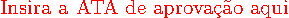
\includepdf{ata_de_aprovacao}
  % ----------------------------------------------------------------------------------------------------- %
  \dedication{A algu\'em cujo valor \'e digno desta dedicat\'oria.}

  \begin{acknowledgement}
Agradeço sinceramente a todos que contribuíram para a realização deste trabalho de conclusão de curso.

Primeiramente, gostaria de agradecer à Deus por todas as oportunidades que tenho diariamente de crescer e pelo dom da vida que nos foi dado. Gostaria de expressar minha gratidão à minha orientadora/professora Glenda, cuja orientação e apoio foram fundamentais para o desenvolvimento deste trabalho. Principalmente, pela paciência que sempre teve durante meus (muitos) dias de procrastinação.

Também gostaria de agradecer à minha família, por simplesmente estarem sempre lá por mim. À minha mãe, meu pai e meus dois irmãos: sem vocês eu nada seria e nem mesmo teria algo pelo qual lutar, amo vocês. E claro, aos meus gatos, que também são parte essencial da família, hahaha.

Agradeço aos meus grandes amigos e colegas de curso, que covardemente não me esperaram para formarmos juntos (risos), mas sempre contribuíram com nossos debates construtivos e aquelas grandes saidinhas para o bar da esquina, que acreditem, é fundamental para um universitário sobreviver...

Além disso, gostaria de expressar minha gratidão a todas as instituições, professores e pesquisadores cujo trabalho e estudos foram referências importantes para este projeto.

Este trabalho não teria sido possível sem a existência de cada um dos que foram mencionados acima, direta ou indiretamente. Muito obrigado por fazerem parte desta jornada e por ajudarem a tornar este projeto uma realidade.

Atenciosamente,

Ítalo Machado Vilarino.
  \end{acknowledgement}

  \begin{abstract}
O crescimento da temperatura global é um fato alarmante. Segundo a \emph{World Meteorological Organization}~\cite{wmo2021}, o ano de 2020 atingiu uma média histórica de \SI{1,2}{\degree C} acima das temperaturas aferidas na era pré-industrial. Aragão \emph{et al.}~\cite{aragao2018amazon} documentam que, desde o início do século~XXI, o fogo associado à seca passou a \emph{neutralizar} os ganhos obtidos com a redução do desmatamento na Amazônia; Silva-Junior \emph{et al.}~\cite{silvajunior2025amazon} mostram que 2024 marcou a pior degradação por fogo em mais de duas décadas --- \SI{3,3}{\mega\hectare} queimados (\(+400\%\) em relação aos 2 anos anteriores), com emissão estimada de \SI{791}{\mega\tonne} de CO$_{2}$. A preservação das áreas verdes é crucial para mitigar este cenário, e ferramentas de previsão automatizadas, baseadas em aprendizado de máquina, representam uma abordagem promissora.

Este trabalho desenvolve um sistema de \textbf{previsão da ocorrência de fogo observado} na Amazônia Legal. A partir de mais de \num{900000} focos ativos do Programa Queimadas/INPE (2014--2023), formula-se um problema de classificação bem-posto sobre uma grade regular de \SI{0,25}{\degree} $\times$ mês: para cada célula propensa a fogo, prevê-se se haverá foco no mês seguinte (\(t+1\)), com \textbf{classe negativa real} (células-mês sem foco) --- corrigindo a limitação de bases \emph{presence-only}, em que só existem registros de fogo. O conjunto final tem \num{450144} células-mês (prevalência do alvo de \SI{24,7}{\percent}). As \emph{features} são \textbf{estritamente causais} (apenas informação até \(t\): histórico de fogo defasado, sazonalidade, climatologia local e desmatamento recente PRODES/DETER), e a avaliação emprega \textbf{validação espaço-temporal em bloco}~\cite{roberts2017cv} --- \emph{rolling-origin} por ano e \emph{leave-region-out} ---, que evita o otimismo do \emph{split} aleatório em dados geográficos.

O modelo (\emph{Histogram-based Gradient Boosting}~\cite{friedman2001greedy}) atinge \textbf{\num{0,777} de PR-AUC} na validação temporal e \num{0,759} na espacial, superando as linhas de base de \emph{persistência} (\num{0,449}) e \emph{climatologia} (\num{0,715}). No \emph{benchmark} contra índices físicos operacionais, avaliados sobre \emph{fogo observado} nas mesmas amostras, o modelo (\num{0,858}) \textbf{supera} tanto o \emph{Fire Weather Index} canadense (\num{0,608})~\cite{vanwagner1985fwi} quanto o índice Risco de Fogo do INPE (\num{0,398}) --- evidenciando o ganho do aprendizado de máquina sobre os índices meteorológicos que a literatura toma como referência operacional. A incerteza é quantificada por \emph{conformal prediction}~\cite{sadinle2019lac} (cobertura empírica de \SI{88,8}{\percent}), a robustez é confirmada por comparação entre famílias de modelo com intervalos de confiança, e experimentos controlados de covariáveis identificam o \textbf{desmatamento recente} (PRODES/DETER) como o principal sinal preditivo da \emph{nova ignição} --- coerente com a natureza majoritariamente antrópica do fogo amazônico~\cite{aragao2018amazon}. O sistema é exposto por uma aplicação web interativa (\emph{Flask} + \emph{Folium}~\cite{folium,leafletjs}) que mapeia a probabilidade de fogo por célula, com rótulo conformal e integração de clima (NASA POWER~\cite{nasapower}) e focos ativos (NASA FIRMS~\cite{nasafirms}) em tempo quase-real. Uma etapa exploratória inicial --- a classificação supervisionada do índice de risco do INPE em faixas de severidade, cuja circularidade metodológica (o alvo era a saída de outro modelo) motivou a reformulação aqui adotada --- é documentada como material complementar.
  \end{abstract}

  \begin{foreignabstract}
The alarming rise in global temperatures is an undeniable reality. According to the World Meteorological Organization~\cite{wmo2021}, the year 2020 witnessed a historical average temperature increase of \SI{1.2}{\degree C} above pre-industrial levels. Aragão \emph{et al.}~\cite{aragao2018amazon} document that, since the beginning of the 21st century, drought-related fires have started to \emph{offset} the gains obtained from reductions in Amazon deforestation; Silva-Junior \emph{et al.}~\cite{silvajunior2025amazon} report that 2024 marked the worst fire-driven degradation event in over two decades --- \SI{3.3}{\mega\hectare} burned (\(+400\%\) over the previous two years), with estimated emissions of \SI{791}{\mega\tonne} of CO$_{2}$. Preserving forested areas is therefore crucial, and automated prediction tools based on machine learning represent a promising approach.

This work develops a system for \textbf{predicting observed fire occurrence} in the Brazilian Legal Amazon. From over \num{900000} active-fire detections of the INPE Fire Programme (2014--2023), a well-posed classification problem is formulated on a regular \SI{0.25}{\degree} $\times$ month grid: for each fire-prone cell, the model predicts whether a fire detection will occur in the following month (\(t+1\)), with a \textbf{real negative class} (cell-months without fire) --- correcting the limitation of \emph{presence-only} datasets that contain fire records only. The final set has \num{450144} cell-months (target prevalence \SI{24.7}{\percent}). Features are \textbf{strictly causal} (only information up to \(t\): lagged fire history, seasonality, local climatology, and recent PRODES/DETER deforestation), and evaluation uses \textbf{blocked spatio-temporal validation}~\cite{roberts2017cv} --- yearly \emph{rolling-origin} and \emph{leave-region-out} ---, which avoids the optimism of random splits on geographic data.

The model (\emph{Histogram-based Gradient Boosting}~\cite{friedman2001greedy}) reaches \textbf{\num{0.777} PR-AUC} in temporal validation and \num{0.759} in spatial validation, outperforming the \emph{persistence} (\num{0.449}) and \emph{climatology} (\num{0.715}) baselines. In a \emph{benchmark} against operational physical indices, evaluated on \emph{observed} fire over the same samples, the model (\num{0.858}) \textbf{outperforms} both the Canadian \emph{Fire Weather Index} (\num{0.608})~\cite{vanwagner1985fwi} and the INPE Fire Risk index (\num{0.398}) --- evidencing the added value of machine learning over the meteorological indices the literature adopts as an operational reference. Uncertainty is quantified via \emph{conformal prediction}~\cite{sadinle2019lac} (empirical coverage \SI{88.8}{\percent}), robustness is confirmed by a confidence-interval comparison across model families, and controlled covariate experiments identify \textbf{recent deforestation} (PRODES/DETER) as the main predictive signal for \emph{new ignitions} --- consistent with the predominantly anthropogenic nature of Amazon fire~\cite{aragao2018amazon}. The system is exposed through an interactive web application (\emph{Flask} + \emph{Folium}~\cite{folium,leafletjs}) that maps per-cell fire probability, with a conformal label and near-real-time climate (NASA POWER~\cite{nasapower}) and active-fire (NASA FIRMS~\cite{nasafirms}) integration. An initial exploratory stage --- the supervised classification of the INPE risk index into severity bands, whose methodological circularity (the target was another model's output) motivated the reformulation adopted here --- is documented as supplementary material.
  \end{foreignabstract}
  \printlosymbols
  \printloabbreviations
  % ---- Cria a lista de figuras. OPCIONAL
  \listoffigures
  % ---- Cria a lista de tabelas. OPCIONAL
  \listoftables
  % ---- Cria o sumário. OBRIGATÓRIO
  \tableofcontents % sumário
% --- Marca o inicio dos elementos textuais. Capítulos.
\mainmatter
% ---- Defino o espaçamento de um e meio centímetros
\onehalfspacing
% ----------------------------------------------------------------------------------------------------- %
% Capítulos do trabalho
% ----------------------------------------------------------------------------------------------------- %
\ChapterStart{first}{First chapter}
\chapter{Introdução}

``Tempo seco e altas temperaturas são fatores que favorecem o aumento de incêndios ambientais'' \cite{Silva21}. Em tempos como os atuais, faz-se ainda mais necessário encontrar ferramentas que auxiliem a frenagem destes eventos. Recentemente, o Instituto Nacional de Metereologia (INMET) emitiu diversos alertas sobre as ondas de calor que viriam a atingir algumas regiões do país. Como consequência o segundo semestre do ano de 2023, em especial os meses de agosto à novembro, registraram um recorde histórico na média de temperaturas, conforme exposto na reportagem publicada pelo próprio instituto, ``Temperatura média atinge recorde no Brasil pelo quarto mês seguido'' \cite{inmet23:ondadecalor}.

Os prejuízos causados por incêndios e queimadas, principalmente quando se trata da Amazônia, que é considerada por muitos como o pulmão do mundo, são diversos. Silva (\citeyear{Silva21}) argumenta como estes eventos introduzem um processo de degradação do solo, perda de matéria-prima e poluição do ar, desencadeando impactos devastadores que reverberam além das fronteiras da floresta, afetando ecossistemas globais e sendo gerador de prejuízos econômicos com uma magnitude preocupante.

Estes danos, apesar de já se mostrarem severos, podem ir muito além. Muitos estudos evidenciam que a nossa participação na emissão de gases, como o dióxido de carbono, alavancam o fenômeno de aquecimento global. Existem, claro, opiniões sobre o tema que se contrapõem e devem ser consideradas. Segundo a reportagem ``Aquecimento global: quem é culpado?" \cite{Aguiar13}, o efeito estufa é uma realidade inegável, mas a dúvida paira sobre a real contribuição do homem neste âmbito. Caso o aquecimento global antropogênico seja factual, as incidências de queimadas corroboram para o cenário atual, o que torna ainda mais importante o estudo e a prevenção das mesmas.

A utilização de agentes inteligentes (como máquinas de aprendizado) para este escopo de pesquisa representa uma abordagem promissora no campo da gestão ambiental e prevenção de desastres. Os modelos de aprendizado de máquina são sistemas computacionais inspirados na racionalidade humana, capazes de aprender padrões complexos a partir de dados. Ao serem aplicadas na previsão de incêndios florestais, esses agentes podem ter a capacidade de assimilar grandes volumes de informações (por exemplo, no espectro de Redes Neurais Artificiais), considerando variáveis ambientais, climáticas e históricas. De acordo com o modelo utilizado pode-se ter flexibilidade na modelagem da sua arquitetura, o que permite a adaptação a padrões não-lineares presentes nos dados, objeto fundamental para modelar a dinâmica complexa dos incêndios florestais \cite{Ferneda06}.

Treinar um modelo com conjuntos de dados históricos que contêm informações detalhadas sobre a topologia e vegetação de uma região é um desafio desde o tratamento dos dados até a avaliação dos mesmos. A realização deste projeto busca desenvolver uma inteligência apta a reconhecer similaridades sutis e correlações que podem ser cruciais na identificação das áreas propensas a incêndios. O uso desse tipo de tecnologia pode ser útil às unidades competentes, contribuindo com o enfrentamento da degradação ambiental por meio de um mapa de risco capaz de orientar sobre as áreas que possuem mais suscetibilidade a combustão. Assim, a proposta é ser capaz de obter um sistema eficiente e de baixo custo computacional para a previsão de incêndios em um ambiente com uma grande quantidade de dados disponíveis.

\section{Justificativa}

O monitoramento de incêndios florestais é uma tarefa que transita entre os espectros de previsão sobre o risco de fogo e a detecção em tempo real. Prever é frequentemente considerado mais interessante ou valioso do que simplesmente detectá-los após o início de uma incidência, por várias razões. Primeiro, permite que medidas preventivas sejam tomadas antes mesmo do início do fogo. Isso pode incluir a alocação mais eficiente de recursos de combate a incêndios e decisões de gestão florestal a longo prazo, como o planejamento de zonas de proteção em torno de áreas sensíveis.

Além disso, prever incêndios pode simplesmente ajudar a reduzir as perdas econômicas associadas a danos à propriedade, perda de colheitas e interrupção de atividades comerciais. Isso é especialmente importante em áreas onde a agricultura, o turismo e outras atividades econômicas dependem da saúde dos ecossistemas naturais. Do outro lado da moeda, um dos principais benefícios de sistemas de detecção é a capacidade de identificar incêndios em estágios iniciais. Isso permite uma resposta rápida e eficaz para conter o fogo antes que ele se espalhe e cause danos significativos. Em suma, pode-se dizer que tanto a detecção quanto a previsão de incêndios são importantes; a capacidade de detectá-los fornece uma resposta rápida e eficaz, enquanto a de prevê-los oferece uma gama mais ampla de benefícios, desde a prevenção completa de danos até a redução de perdas econômicas.

A urgência do tema é corroborada por publicações recentes na literatura internacional. Aragão \emph{et al.}~\cite{aragao2018amazon} documentaram, no periódico \emph{Nature Communications}, que desde o início do século~XXI o fogo associado à seca passou a \emph{neutralizar} os ganhos obtidos com a redução do desmatamento na Amazônia. Mais recentemente, Silva-Junior \emph{et al.}~\cite{silvajunior2025amazon}, em \emph{Biogeosciences}, mostraram que 2024 marcou a pior degradação por fogo em mais de duas décadas: \SI{3,3}{\mega\hectare} queimados (acréscimo de \(\approx 400\%\) em relação aos dois anos anteriores), com emissão estimada de \SI{791}{\mega\tonne} de CO$_{2}$. Esses números reforçam a urgência operacional do desenvolvimento de ferramentas modernas de previsão e vigilância, capazes de produzir mapas de risco em tempo quase-real e auditáveis por gestores ambientais.

Dada a magnitude e complexidade das queimadas na região da Amazônia, abordagens eficientes para prevenção, monitoramento e resposta rápida são cruciais. A utilização de agentes inteligentes para mapear focos de incêndio não é uma novidade, contudo, dadas as especificidades de cada região atacada, diferentes variáveis podem se destacar nos algoritmos para a previsão dos focos. Além disso, deve-se considerar o contexto global das mudanças climáticas e o impacto direto que possuem as queimadas sobre a vegetação e biodiversidade amazônica nessas alterações. Isto posto, este projeto deve instituir uma base de conhecimento sólida, integrando conceitos de sensoriamento remoto e aprendizado de máquinas na intenção de entender e mitigar os efeitos adversos dos incêndios florestais.


\section{Objetivos}

\subsection{Objetivo Geral}

Desenvolver e validar um sistema de aprendizado de máquina para a \textbf{previsão da ocorrência de fogo observado} na Amazônia Legal, estimando, para cada célula de uma grade regular, a probabilidade de haver foco de incêndio no mês seguinte, e demonstrar seu ganho preditivo frente aos índices de risco meteorológicos operacionais (\emph{Fire Weather Index} e Risco de Fogo do INPE).

\subsection{Objetivos Específicos}

\begin{itemize}
    \item[1.] Realizar uma revisão bibliográfica sobre a previsão de ocorrência de incêndios florestais e o estado da arte em aprendizado de máquina aplicado a fogo, incluindo trabalhos de 2022--2025 sobre validação espaço-temporal, previsão de fogo observado e quantificação de incerteza.
    \item[2.] Construir um conjunto de dados de ocorrência bem-posto sobre uma grade regular de \SI{0,25}{\degree} $\times$ mês, definindo a presença por focos observados do Programa Queimadas/INPE e uma \textbf{classe negativa real} (células-mês sem foco), a partir de mais de \num{900000} focos registrados na última década (2014--2023).
    \item[3.] Realizar a engenharia de \emph{features} \textbf{estritamente causais} (apenas informação disponível até o instante \(t\)): histórico de fogo defasado, sazonalidade, climatologia local e \emph{drivers} antrópicos de desmatamento (PRODES/DETER), evitando o vazamento temporal.
    \item[4.] Treinar e comparar modelos de aprendizado de máquina (\emph{gradient boosting} e famílias alternativas) sob \textbf{validação espaço-temporal em bloco} (\emph{rolling-origin} por ano e \emph{leave-region-out})~\cite{roberts2017cv,bergmeir2012cv}, tendo o PR-AUC como métrica primária e as linhas de base de \emph{persistência} e \emph{climatologia} como referência mínima de desempenho.
    \item[5.] Realizar o \emph{benchmark} do modelo contra os índices físicos operacionais (\emph{Fire Weather Index} canadense~\cite{vanwagner1985fwi} e Risco de Fogo do INPE) sobre fogo \emph{observado}; quantificar a incerteza por \emph{conformal prediction}~\cite{sadinle2019lac}; e analisar a contribuição das variáveis, com destaque para o papel do desmatamento recente na \emph{nova ignição}.
    \item[6.] Disponibilizar os resultados em uma \textbf{aplicação web interativa} (\emph{Flask} + \emph{Folium}~\cite{folium,leafletjs}) que apresente, por célula, a probabilidade de fogo no próximo mês, o rótulo conformal de confiança e os principais \emph{drivers} associados, viabilizando o uso operacional por gestores ambientais.
\end{itemize}

\section{Estrutura da Monografia}

Este trabalho está organizado em sete capítulos que abordam diferentes etapas da pesquisa, proporcionando uma compreensão abrangente do desenvolvimento do sistema de previsão de queimadas na Amazônia.

\textbf{2. Estado da Arte:} são explorados trabalhos correlatos e avanços significativos na área de previsão de queimadas, com foco em estudos que propõem o mapeamento de regiões suscetíveis a fogo. A revisão aborda a extensão do problema considerando seus impactos ambientais, sociais e econômicos. Adicionalmente, são examinadas abordagens tradicionais de aprendizado de máquina e o início dos sistemas de prevenção, complementadas por uma seção de \textbf{literatura recente 2024--2025} (\emph{ensembles} explicáveis, índice KBDI no Cerrado-Amazônia, validação temporal estrita).

\textbf{3. Fundamentação Teórica:} estabelece as bases conceituais necessárias para a compreensão do problema das queimadas na Amazônia. Inicia-se com a contextualização do bioma amazônico e a problemática dos incêndios florestais, seguida pela discussão do sensoriamento remoto e das tecnologias espaciais. O capítulo prossegue com os fundamentos da inteligência artificial e do aprendizado de máquina, contemplando \textbf{modelos clássicos} (Regressão Logística, Random Forest), \textbf{modelos modernos de \emph{boosting}} (XGBoost, LightGBM, CatBoost), \textbf{\emph{ensembles}} (Voting e Stacking), \textbf{otimização de hiperparâmetros} (Optuna), \textbf{interpretabilidade} (SHAP e Permutation Importance), \textbf{tratamento de desbalanceamento}, \textbf{calibração de probabilidades}, \textbf{índices físico-climáticos de fogo} (KBDI, SPI, VPD, De Martonne) e \textbf{validação temporal} de modelos.

\textbf{4. Metodologia:} descreve detalhadamente os passos e procedimentos adotados para desenvolver o sistema de previsão. São delineados os métodos de coleta e enriquecimento dos dados (Programa Queimadas + NASA POWER + NASA FIRMS), o pré-processamento, a engenharia das 24~\emph{features} Tier~1, o protocolo de treinamento dos modelos, a avaliação (métricas, interpretabilidade, \emph{threshold tuning}, validação temporal), e o desenvolvimento da aplicação web interativa explicável.

\textbf{5. Estudo Exploratório (baseline):} apresenta uma primeira abordagem, na qual se classificou o índice de Risco de Fogo do INPE em faixas de severidade. Documenta o comparativo entre as oito abordagens treinadas, a interpretabilidade (SHAP e \emph{Permutation Importance}), a validação temporal estrita e o estudo de caso externo (Pium--TO / CENSIPAM). Este capítulo é apresentado como \textbf{baseline exploratório}: a constatação de que o alvo era a saída de outro modelo (circularidade metodológica) motivou a reformulação central do trabalho, no Capítulo~6.

\textbf{6. Previsão de Ocorrência de Fogo (contribuição central):} constitui o núcleo do trabalho. Reformula o problema para a \textbf{previsão de fogo observado} (mês~\(t+1\)) com classe negativa real, \emph{features} causais e validação espaço-temporal em bloco. Apresenta o desempenho frente a linhas de base, a comparação entre famílias de modelo com intervalos de confiança, o \textbf{benchmark contra índices físicos} (FWI canadense e Risco de Fogo INPE), a quantificação de incerteza por \emph{conformal prediction}, os \textbf{drivers antrópicos de desmatamento} (PRODES/DETER) e a validação do rótulo contra a área queimada do MapBiomas Fogo.

\textbf{7. Conclusão:} sintetiza os principais achados, registra as limitações reconhecidas e enumera os trabalhos futuros prioritários para evoluir o sistema rumo à integração de novas fontes (NDVI/EVI MODIS, MapBiomas Fogo) e de causalidade estrita nas \emph{features} de janela móvel.

\chapter{Estado da Arte}

No capítulo de Estado da Arte serão explorados e analisados trabalhos correlatos que se destacam na literatura científica em relação ao tema proposto. Este capítulo fornecerá uma base de revisões e críticas das abordagens existentes para a previsão utilizando aprendizado de máquina, com foco em incêndios florestais e relatando, especialmente, estudos que envolvem a análise empírica e estatística dos dados para correlacionar as ocorrências e os eventos que se fazem presente. Serão apresentadas contribuições significativas, metodologias inovadoras, e resultados obtidos por pesquisadores que exploraram o emprego de técnicas avançadas de inteligência artificial na antecipação destes eventos.

\section{Trabalhos Correlatos}

Os trabalhos de previsão de incêndios florestais dividem seus esforços em dois principais métodos de análise, que de um lado consistem na utilização de modelos matemáticos e estatíscos e do outro, no Aprendizado de Máquinas.

A previsão baseada em estatísticas ocorre por meio da correlação dos parâmetros metereológicos registrados nos incêndios históricos, tais como condições climáticas, terreno, temperatura média, pressão circunstancial e a frequência de incêndios que estes fatores causam ao ambiente. Pradeep et al.~\cite{pradeep2022eravikulam} utilizaram um Sistema de Informação Geográfica (SIG) para delinear as zonas de risco de incêndios florestais no Parque Nacional Eravikulam, na Índia, por meio dos métodos de Processo Analítico Hierárquico (AHP) e a Razão de Frequência (FR), chegando a categorizar 72\% e 24\%, respectivamente, das incidências de incêndio na zona de alto risco dos mapas preparados. Gülçin e Deniz~\cite{gulcin2020manisa} também elaboraram um mapa de risco de incêndio, dessa vez na província de Manisa, na Turquia, e utilizaram técnicas baseadas em Sensoriamento Remoto (SR) e SIG, reportando que 25,8\% da área de estudo apresentava risco alto ou muito alto de combustão espontânea.

A velocidade de propagação do fogo e a proporção do alcance do mesmo dependem fortemente da topografia e a arborização da região. Jin e Lee~\cite{jin2022northkorea} realizaram um estudo sobre as características de incêndios florestais em duas províncias da Coréia do Norte (South Hamgyong e Gangwon) e concluíram que as árvores coníferas são muito mais suscetíveis à combustão em relação às demais plantas da região. Além disso, os resultados mostraram que a maioria dos grandes incêndios ocorreu ao longo de encostas abertas a favor do vento. Xu et al.~\cite{xu2016hubei} realizaram um estudo para relacionar os danos ao corredor das linhas de energia de Hubei, na China, com as incidências de incêndios florestais nas suas proximidades. Os resultados foram obtidos a partir da implementação de um modelo de Regressão Logística para prever as ocorrências de incêndio e sua correlação com os desligamentos da linha, cruzando dados históricos e topográficos.

No que tange a previsão a partir de dados tabulares, os métodos de Aprendizado de Máquina que se mantém em evidência são os modelos mais tradicionais, como Regressão Logística, Floresta Aleatória e \textit{Suport Vector Machine} (SVM). Kalantar et al.~\cite{kalantar2020forest} previu a suscetibilidade de incêndios florestais na bacia hidrográfica de Chaloos Rood, no Irã, aplicando três modelos de aprendizado de máquina à um conjunto de 14 variáveis preditoras, que derivaram das características climáticas, ambientais e topográficas da região. Destaque para o modelo de \textit{boosted regression tree} (BRT), que superou os outros dois de forma geral, alcançando os maiores índices de Área Sob Curva (AUC) na métrica de desempenho. Tien Bui et al.~\cite{tienbui2016tropical} propôs a utilização de um modelo de aprendizado promissor para a classificação binária de suscetibilidade de fogo, chamado \textit{Kernel Logistic Regression} (KLR). A avaliação foi realizada nas proximidades do Parque Nacional Cat Ba, no Vietnã. De forma simplista, o algoritmo é capaz de mapear o conjunto de entrada de maneira linear e atribui um "peso" de influência para cada uma das características sobre o resultado final e, neste estudo, foi capaz de alcançar resultados extremamente satisfatórios. Para título de comparação, foi utilizada uma SVM de referência nesta mesma base dados e com os mesmos parâmetros do modelo proposto, e os resultados descriminaram uma leve vantagem no desempenho do modelo KLR.

Na província de Heilongjiang, Chang et al.~\cite{chang2013predicting} utilizaram regressão logística para criar um mapa de probabilidade de ignição. Com uma proposta um pouco mais específica, este trabalho categorizou os incêndios entre antropogênicos (causados por humanos) e naturais. Dessa forma, a importância que as variáveis dependentes possuíam foi determinada a partir das correlações identificadas na incidência de cada um dos tipos de fogo. Concluiu-se na região estudada que os incêndios naturais possuem uma forte relação com a média anual de temperatura, enquanto que a variável mais influente para incêndios antropogênicos é o tipo de vegetação. Bisquert et al.~\cite{bisquert2012application} classificaram os seus resultados em três níveis de suscetibilidade. Para isso, utilizou-se o modelo de regressão logística para identificar as variáveis de maior importância dentre os verdadeiros positivos e, posterior à essa classificação, estes dados foram inseridos em um algoritmo de Rede Neural Artificial, atribuindo três possíveis saídas aos rótulos do modelo (de menor à maior risco de fogo).

Al-Bashiti e Naser~\cite{albashiti2022wildfire} exploraram uma variedade de modelos de aprendizado de máquina, entre eles algoritmos de aprendizado profundo e árvore de decisão que apresentaram uma precisão superior a 80\% em bases de dados extremamente grandes. Além disso, os algoritmos genéticos também foram efetivos na previsão do tamanho esperado dos incêndios, também com margem de precisão acima de 80\%. A pesquisa concluiu que as performances atingidas tem uma ligação direta com a qualidade das observações dos incêndios que são documentados, tais como dados históricos, do clima e relevo. Malik et al.~\cite{malik2021datadriven} propuseram duas abordagens para o aprendizado de risco de incêndio. A primeira, a qual foi denominada modelo de conjunto, utiliza dois modelos base para segregar o conjunto de variáveis em escopos e, com os resultados alcançados nestes blocos, seguir para um novo treinamento. O modelo de conjunto se provou incapaz de derivar as relações entre as variáveis independentes para atingir resultados mais concisos. A segunda abordagem utilizou apenas um modelo que recebeu um conjunto completo dos dados selecionados, chamado de modelo combinado. Este segundo experimento revelou um agente capaz de deduzir efetivamente relações entre as variáveis independentes, uma vez que elas foram testadas em conjunto, e alcançou precisão superior a 90\%.

Pode-se segmentar o monitoramento de incêndios florestais em dois grandes espectros: a previsão, que determina as áreas de risco e antecede as medidas preventivas; e a detecção, que viabiliza o monitoramento em tempo real e visa distinguir os incêndios reais de maneira pontual. Pode-se dizer que as pesquisas voltadas para previsão e detecção estão fortemente ligadas enquanto finalidade (prevenção de incêndios), mas se dissociam nas metodologias, modelos e resultados esperados. Todos os estudos supracitados baseiam-se no reconhecimento estatístico de padrões históricos de queimadas, mas quando cita-se monitoramento de incêndios, não se pode deixar de lado estudos que visam reconhecer o fogo por meio da visão computacional. Jin et al.~\cite{jin2024swvr} propuseram um modelo de Aprendizado Profundo através da combinação de duas arquiteturas tradicionais: o \textit{lightweigth vision transformer} (ViT) e as Redes Neurais Convolucionais (CNN's). O objetivo desta combinação era otimizar os resultados na detecção de incêndios florestais, diminuindo a complexidade computacional e conservando a perfomance dos algoritmos tradicionais. O SWVR, como foi chamado o modelo proposto, alcançou uma precisão de 79,6\% na identificação de incêndios reais. Além disso, foi capaz reduzir o custo computacional do modelo de referência em quase 37\%.

\subsection{Literatura recente (2024--2025)}

A última década consolidou o uso de \emph{ensembles} de árvores e métodos de interpretabilidade como prática essencial em estudos de suscetibilidade a incêndios florestais. Três tendências contemporâneas merecem destaque por nortearem as decisões metodológicas deste trabalho.

\paragraph{Interpretabilidade via SHAP e \emph{Permutation Importance}.} Cheerala \emph{et al.}~\cite{cheerala2025probabilistic} aplicaram \emph{Random Forest} combinado com SHAP~\cite{lundberg2017unified} em regiões de \emph{grassland} e \emph{forest} da Califórnia, obtendo AUC de \num{0,996} e \num{0,997} respectivamente, com identificação clara das \emph{features} dominantes (NDVI, EVI, histórico de fogo, umidade do combustível). Vasconcelos \emph{et al.}~\cite{forests2024cerradoamazon} identificaram o índice KBDI (\emph{Keetch-Byram Drought Index})~\cite{keetch1968drought} como o melhor preditor de fogo em Canaã dos Carajás (Pará), na zona de transição Cerrado--Amazônia. Quesada-Ruiz \emph{et al.}~\cite{npjhazards2025fire}, em \emph{npj Natural Hazards}, propuseram um modelo híbrido (componente dinâmica do ECMWF + \emph{Random Forest}) que utiliza o SPI~\cite{mckee1993spi} observado para prever anomalia de área queimada com até um mês de antecedência em \(\approx 68\%\) das áreas queimáveis brasileiras. Esses trabalhos motivam, na presente pesquisa, a adoção combinada de KBDI \emph{proxy}, VPD \emph{proxy}~\cite{seager2015climatology} e SPI multi-escala como \emph{features} Tier~1 do \emph{pipeline} (Capítulo~\ref{cap:metodologia}).

\paragraph{Validação temporal e \emph{drift} climático.} Bergmeir \& Benítez~\cite{bergmeir2012cv} alertam que o uso de \emph{cross-validation} estratificada padrão em séries temporais introduz viés otimista, sendo necessário utilizar \emph{rolling-origin} ou \emph{TimeSeriesSplit}. Esta recomendação é tomada como princípio metodológico no Apêndice~\ref{cap:resultados} deste trabalho. A relevância prática desse cuidado é amplificada por Silva-Junior \emph{et al.}~\cite{silvajunior2025amazon}, que documentam 2024 como o pior ano de degradação por fogo na Amazônia em mais de duas décadas (\SI{3,3}{\mega\hectare}), justificando o uso de janelas temporais recentes (2021--2023) como teste mais desafiador --- período em que os modelos devem provar robustez sob \emph{drift} climático real.

\paragraph{\emph{Pseudo-labeling} para imputação climática.} Lopez-Garcia \emph{et al.}~\cite{lopezgarcia2024spatiotemporal} aplicaram \emph{pseudo-labeling}~\cite{lee2013pseudo} para imputar dados SMAP em \emph{grids} tropicais, com regressor supervisionado atingindo \(R^2 > 0{,}90\) em \emph{holdout}. A mesma estratégia é adotada neste projeto (Seção~\ref{sec:metodologia_pseudo_label}) para imputar a variável \texttt{Umidade} nos \num{763489} registros não enriquecidos via NASA POWER, com cuidados explícitos quanto ao viés de confirmação relatados por Arazo \emph{et al.}~\cite{arazo2020pseudo}.

\paragraph{Fusão estação--grade, \emph{fire weather} e ambiguidade operacional.} Revisões recentes enfatizam variáveis dinâmicas de combustível e meteorologia de superfície (precipitação local, déficit de umidade, temperatura máxima, vento) como condicionantes de propagabilidade, frequentemente sintetizadas em índices de \emph{fire weather}. Em paralelo, a literatura de observação da Terra discute quantificação de incerteza preditiva --- ainda raramente operacionalizada em painéis acadêmicos. Estas tendências motivam extensões ao \emph{pipeline} de serviço documentadas na Seção~\ref{sec:res_estudo_caso_pium} (subsubseção~M4): busca hierárquica de estações INMET com rótulo de representatividade, vento WIS2 alinhado à precipitação da mesma estação, variáveis NASA POWER adicionais expostas na API, indicador escalar de \emph{fire weather} e métricas FNR/FPR na auditoria contra FIRMS --- implementadas de modo a não alterar o pré-processador de treino até um retreino controlado, evitando \emph{train/serve skew}.

\paragraph{Previsão de \emph{ocorrência observada} e validação espaço-temporal.} Uma vertente recente distingue-se por prever o \emph{fenômeno observado} (focos ou área queimada), e não a saída de um índice. Huot \emph{et al.}~\cite{huot2022nextday} consolidaram o \emph{benchmark} \emph{Next Day Wildfire Spread}, que prevê a máscara de fogo observada do dia seguinte; Karasante \emph{et al.}~\cite{karasante2025firecastnet} propuseram o \emph{FireCastNet} (\emph{earth-as-a-graph}) para previsão sazonal de área queimada sobre grade de \SI{0,25}{\degree}; de Andrade \emph{et al.}~\cite{deandrade2024lstmgru} modelaram focos mensais na Amazônia com redes LSTM/GRU. No plano operacional, o sistema GEFF/EFFIS do Copernicus opera o \emph{Fire Weather Index} canadense em previsão dirigida por modelos numéricos~\cite{digiuseppe2024geff}. Metodologicamente, Roberts \emph{et al.}~\cite{roberts2017cv} estabelecem a validação em blocos espaço-temporais como padrão para dados geográficos, e a quantificação de incerteza por \emph{conformal prediction}~\cite{mortier2024conformal,sadinle2019lac} ganha tração em observação da Terra. Essas referências fundamentam a reformulação do problema apresentada no Capítulo~\ref{cap:ocorrencia}.

Em resumo, a bibliografia discutida destaca o amplo espectro de abordagens e tecnologias disponíveis para mitigar o impacto devastador dos incêndios florestais. Desde métodos tradicionais, como modelos baseados em dados históricos e estatística, até avanços recentes em inteligência artificial e aprendizado de máquina, a pesquisa nesse campo está constantemente evoluindo. Destaca-se, nesta área, a importância de uma base de dados sólida e composta por múltiplas fontes, incluindo informações meteorológicas, dados geoespaciais e situação climática, que podem contribuir fundamentalmente para melhorar a precisão das previsões. Além disso, apesar de não ser parte do escopo desta pesquisa, técnicas avançadas, como o uso de redes neurais convolucionais e algoritmos de aprendizado profundo, tem entregue grandes expectivas na identificação precoce de áreas queimadas e na mensuração de propagação do fogo.

\chapter{Fundamentação Teórica}

Este capítulo busca apresentar, objetivamente, as informações necessárias para a compreensão deste trabalho. Ao longo das demais seções serão abordados diversos assuntos que se relacionam com as queimadas da Amazônia e com o desafio da implementação de um modelo capaz de prever suas áreas mais suscetíveis a incêndios florestais. Para estar imerso neste conteúdo, será necessário entender a base teórica das tecnologias mais promissoras da área de aprendizado de máquina (AM), os efeitos das queimadas a longo e curto prazo e o quão importante faz-se a compreensão do ambiente para impedir ou diminuir a ocorrência destes eventos.

\section{O Bioma da Amazônia}

Os biomas, geralmente, são definidos pelas características predominantes das formações vegetais de um ambiente \cite{TIMM05}. Eles se categorizam em grandes porções geográficas que são entendidas, portanto, como grupos de organismos semelhantes que podem ser compreendidos como uma unidade, dadas as similaridades. É importante afirmar que, além desta definição, também são relevantes as formas do relevo e condições climáticas da região para conceituar um bioma.

O próprio termo ``bioma'' foi criado pelo ecólogo americano Frederic Clements (\citeyear{clements1916}), o qual foi responsável por estudar as relações existentes em comunidades vegetais e determinar que o comportamento de organismos inseridos em uma dessas comunidades busca a sua perpetuação. Este processo discorre pelo aumento das espécies e a evolução na complexidade de suas relações. O bioma é a concepção fundamental desta comunidade como uma unidade formada por partes semelhantes \cite{TIMM05}.

A compreensão da importância do bioma amazônico parte destas características. Segundo o IBGE (\citeyear{ibge04:mapabioma}), a Amazônia é o maior bioma do Brasil, ocupando um território de mais de quatro milhões de quilômetros quadrados (km²). Um terço de toda a madeira tropical do mundo está localizada na região, que abriga cerca de duas mil e quinhentas espécies de árvores e trinta mil espécies de plantas, 30\% do total existente na América do Sul.

\section{Queimadas e Incêndios Florestais}

Desde a década de 90, a região da Amazônia sofre de um  aumento em ataques e queimadas às suas áreas verdes. Segundo FEARNSIDE (\citeyear{fearnside06}), esta tendência é causada, principalmente, pelo pico de desmatamento alcançado durante a instituição do Plano Real, em 1995, e às políticas de incentivo econômico que emergiram sem uma responsabilidade ambiental adequada na mesma época. Em 2005, com a promoção da ``Operação Curupira'' atrelada às grandes taxações imbuídas às exportações internacionais, houve uma política de freio e reversão desse cenário que, contudo, não foi capaz de retrair o suficiente a média negativa dessas últimas três décadas.

As queimadas fazem parte da cultura e processo produtivo de pequenos, médios e grandes agricultores \cite{leonel00}. Trata-se de um método econômico e ágil para efetuar a limpeza de grandes pastos, remover árvores e preparar terras para o plantio. Este fenômeno se explica em seus inúmeros benefícios: as cinzas formadas no processo são ricas em nutrientes que fertilizam o solo e podem aumentar a produtividade; o fogo utilizado é capaz de estimular o crescimento de gramíneas forrageiras e matar as ervas daninhas, fatores prejudiciais para um bom cultivo \cite{sodre21}.

A maior parte dos focos de calor mapeados na Amazônia são, portanto, incidências de fogo atribuído pela ação humana. Estas práticas agropastoris que utilizam o fogo de maneira controlada são chamadas de queimadas. Por outro lado, compreende-se como incêndio florestal toda e qualquer incidência de fogo sobre uma área vegetal por meios naturais ou através da negligência dos atores humanos; denomina o processo de combustão espontânea que ocorre, em sua maioria, nos períodos de seca e estiagem de maneira abrupta e desavisada \cite{vigano17,leonel00}.

Segundo o Instituto Nacional de Pesquisas Espaciais (INPE), o Brasil registrou 131.327 queimadas florestais até o oitavo mês de 2019. Cerca de 33\% destas incidências ocorreram na Amazônia, onde foram registrados 43.573 focos. Segundo FLORENZANO (\citeyear{florenzano07}), o Brasil é o responsável por mais de trezentas mil queimadas anualmente, se contabilizados os dados desde a década de oitenta. Este trabalho que cerca o levantamento dos números das queimadas vem sendo realizado até os dias atuais em uma parceria entre o INPE e o Instituto Brasileiro do Meio Ambiente e dos Recursos Naturais Renováveis (IBAMA), por meio de um Programa de Monitoramento de Queimadas e Prevenção e Controle de Incêndios Florestais no Arco do Desflorestamento da Amazônia, também conhecido como PROARCO.

\section{Programa Queimadas}

O Programa Queimadas é um sistema de monitoramento de focos de calor em tempo real, que opera desde 1998 com imagens de satélites, dados meteorológicos e limites políticos oficiais \cite{INPE24}. Dentre as informações que podem ser extraídas estão a posição geográfica do foco, os limites territoriais que ele faz parte, a data e hora da captura, o bioma dominante, a quantidade de dias sem chuva, valor de precipitação, a potência radioativa do fogo e o risco de incêndio no momento capturado. A Figura \ref{fig:BDQueimadas} mostra todos os registros de focos de calor da America do Sul, no dia 25 de março de 2024, por volta das 12 horas no fuso horário de Brasília.

\begin{figure}[ht]
    \centering
    \includegraphics[scale=0.4]{"imagens/Programa Queimadas.png"}
    \caption{Captura de tela realizada no dia 25 de março de 2024 sobre o BDQueimadas, mostrando os focos de calor em tempo real registrados pelo satélite GOES-16 \cite{INPE24}}
    \label{fig:BDQueimadas}
\end{figure}

\section{Sensoriamento Remoto e a Tecnologia Espacial}

``Sensoriamento remoto consiste na aquisição de informação sobre um objeto sem que se entre em contato com ele'' \cite{novo10}. Segundo o autor, essa afirmação é muito ampla enquanto definição dos serviços de monitoramento remoto, dado que pode-se adquirir informação, por exemplo, de um jogo de futebol apenas ouvindo as eufóricas reações de seus espectadores. Uma concepção mais adequada seria, portanto, atribuir o sensoriamento remoto para todo tipo de processo que impõe a utilização de um dispositivo que, mediante a observação, é capaz de inferir os fenômenos que ocorrem na superfície terrestre, a partir de uma análise da interação entre as forças que o circundam (eletromagnéticos, acústicos ou potenciais) e os elementos que constituem esta superfície. O resultado imposto ao ambiente pode ser analisado com diferentes abordagens.

Exemplificando, existem sensores capazes de detectar, por exemplo, ondas sonoras: os sonares. Eles utilizam a teoria de propagação do som para determinar a localização de objetos partindo da premissa que, em meios homogêneos, o som desloca-se em velocidade constante. Portanto, é possível determinar o posicionamento de um objeto com o cálculo da diferença entre a transmissão de um pulso e sua recepção, chamada de eco.

Segundo IGOR (\citeyear{machado17:santos17}) e LIU (\citeyear{liu07}), esta metodologia encontra uma limitação dentro do escopo da tecnologia espacial. Os sensores espaciais, como satélites, restringem-se fundamentalmente às alterações que os objetos impõem ao campo eletromagnético. É apropriado dizer, portanto, que o SR\footnote[1]{Refere-se à abreviação da expressão "Sensoriamento Remoto", a qual estamos frequentemente referenciando neste capítulo.} cabe à todo processo de obtenção de informação que utiliza-se da radiação eletromagnética (REM) e de sua interação com objetos e fenômenos, uma vez que sua detecção é independente de um meio de propagação e menos propensa a ruídos.

A Figura \ref{fig:REM} acompanha a definição de Novo (\citeyear{novo01:ponzoni}), que diz que sensoriamento remoto pode ser conceituado a partir de um esquema que possui três vértices que interagem entre si a partir de uma base em comum, a REM (radiação eletromagnética).

\begin{figure}[ht]
    \centering
    \includegraphics[scale=1]{"imagens/tcc image-SR.png"}
    \caption{Representação dos pilares do Sensoriamento Remoto \cite{novo01:ponzoni}.}
    \label{fig:REM}
\end{figure}

A base de todas as técnicas utilizadas para extrair informações de objetos remotamente está representada neste esquema. A  REM está no centro por tratar do elemento de ligação entre todos os vértices. Acima, tem-se a fonte, geralmente compreendida pelo sol ou a própria terra, a depender do tipo de sensor que vai catalisar o processo de sensoriamento, sendo que toda análise realizada é constituída pela mensuração de REM. Na base inferior esquerda do triângulo está o sensor. De forma sucinta, o sensor é definido como o dispositivo utilizado para captar a REM emitida ou refletida pelo objeto alvo. Uma vez que o alvo é o outro vértice base do triângulo, da qual se pretende extrair a informação, todos se conversam a partir da radiação eletromagnética.

\subsection{Detecção de Focos de Calor}

É fundamental conceituar que os objetos presentes na superfície terrestre emitem e refletem radiação solar. A transformação dessa energia emitida em valores de temperatura é acessível utilizando modelos físicos e, assim, é possível quantificar o calor dos ambientes monitorados. O trabalho do sensoriamento remoto é identificar estes dados que, ao ultrapassar um certo limiar (definido por especialistas), passa a relacionar estas áreas como focos de calor \cite{liu07}.

Focos de calor, a princípio, não são identificados como áreas de incêndio ou queimada. Para um dado ser interpretado como tal, faz-se necessário uma série de eventos geográficos, climáticos e florestais relacionados à região, como informa o autor:

\noindent
\begin{quoting}[rightmargin=0cm,leftmargin=4cm]
\begin{singlespace}
{\footnotesize
Para que um dado foco de calor seja interpretado como um possível foco de fogo, ou ocorrência de incêndio, a informação extraída do satélite precisa ser associada a outras informações em um Sistema de Informações Geográficas (SIG). As informações relevantes a serem associadas precisam ser definidas por meteorologistas (que vão informar se uma dada região apresenta as condições de precipitação, temperatura e umidade favoráveis à ocorrência de incêndio), por Engenheiros Florestais e Biólogos (que vão informar sobre a susceptibilidade da cobertura vegetal à combustão natural ou induzida por queimadas); por Geógrafos (que vão informar sobre a distribuição de usos da terra em diferentes áreas, sobre as práticas agrícolas, culturas dominantes etc.). \cite[p. 32]{novo10}
}
\end{singlespace}
\end{quoting}

Dessa forma, é imprescindível associar não apenas os dados mais concretos e diretos, como também informações menos relevantes e obtidas através de engenharia social para tornar a base de dados mais adequada possível para a análise.

\section{Base de dados}

Uma base de dados (ou banco de dados) é uma coleção organizada de informações ou dados, geralmente armazenados eletronicamente em um sistema de computador. É ideal que estes dados sejam estruturados de forma a permitir o armazenamento, recuperação, modificação e gestão eficientes das informações.

A ideia por trás destes modelos de informação é conter uma ampla variedade de tipos de dados, incluindo textos, números, imagens, áudio, vídeos, entre outros. Esses dados podem representar informações sobre pessoas, produtos, transações, eventos, ou qualquer outra entidade do mundo real que seja relevante para a aplicação em questão.

As bases de dados podem ser organizadas de diversas maneiras, dependendo das necessidades específicas da aplicação. Os tipos mais comuns de bases de dados incluem bases relacionais, NoSQL, orientadas a objetos, distribuídas, entre outras. Cada uma delas possui suas próprias características, estruturas e modelos de armazenamento de dados. Uma estrutura extremamente eficaz para organizar os dados, utilizada principalmente para pesquisas científicas, são as chamadas estruturas de dados tabulares. Os dados tabulares são uma forma comum e eficiente de organizar informações em uma estrutura de linhas e colunas, semelhante a uma planilha.

Existem muitos motivos que justificam a utilização de dados tabulados em pesquisas. Esta forma de organização estruturada fornece um conteúdo fácil de entender, onde cada linha representa uma observação ou exemplo e cada coluna representa uma variável ou atributo. Isso auxilia a interpretação e análise dos dados. Outro fator é que estas estruturas são compatíveis com uma grande variedade de ferramentas e plataformas, o que facilita a manipulação, análise e visualização dos dados. Além disso, podem acomodar uma ampla gama de tipos de dados, incluindo números, texto, datas e categorias. Isso os torna adequados para as tarefas de análise, onde os dados tabulares podem ser facilmente compartilhados e comunicados entre diferentes partes interessadas e são visualmente claros e objetivos.

Trabalhar com dados tabulares requer habilidades em manipulação de dados, análise exploratória, entendimento conceitual dos atributos e interpretação de resultados. Ao dominar essas habilidades, é possível extrair informações valiosas e tomar decisões fundamentadas nos dados fornecidos.

\section{Técnicas de pré-processamento}

A limpeza de dados, também conhecida como pré-processamento de dados, é uma etapa fundamental em qualquer trabalho de classificação e previsão de eventos com \textit{Machine Learning} (ML). Essa etapa envolve a identificação, correção e eliminação de problemas nos dados antes de serem usados para treinar um modelo de ML. Dados sujos ou mal formatados podem prejudicar a qualidade e a precisão de um modelo. Modelos treinados com dados limpos são mais fáceis de interpretar e entender, e isso é especialmente importante em cenários onde é necessário explicar ou justificar as previsões do modelo. Por fim, outro campo altamente influenciado por dados de alta qualidade é a eficiência computacional. Em casos onde há limitação de recursos computacionais, prover dados ``limpos'' para a máquina pode reduzir radicalmente o tempo de treinamento e auxiliar na inferência do modelo.

A presença de ruído, valores ausentes, \textit{outliers} ou inconsistências nos dados pode levar a previsões imprecisas ou enviesadas, tendo um impacto direto nos resultados do modelo. Portanto, é necessário entender os principais problemas conhecidos em dados tabulares e como identificar e realizar o tratamento dos mesmos.

\subsection{Ruídos e \textit{Outliers}}

\textit{Outliers} são pontos de dados que se desviam significativamente do padrão geral de um conjunto de dados. Eles são observações que estão ``longe'' da maioria das outras observações nos dados. A presença de \textit{outliers} pode indicar uma variedade de situações, como erros de medição, flutuações naturais extremas nos dados, ou até mesmo eventos raros ou anomalias que merecem atenção especial.

Entre as principais características dos \textit{outliers} estão os valores extremos, que estão significativamente distantes dos valores típicos ou centrais do conjunto de dados. Eles podem ser muito maiores ou menores do que a maioria dos outros valores e podem distorcer os resultados estatísticos, como média e desvio padrão e, assim, influenciar negativamente a precisão e a interpretação de modelos estatísticos ou de aprendizado de máquina.

Semelhantes aos \textit{outliers}, tem-se os ruídos, que se referem a variações aleatórias ou flutuações nos dados que não estão relacionadas ao fenômeno que está sendo observado. Essas variações aleatórias podem ser introduzidas por uma variedade de razões, como erros de medição, imprecisões nos instrumentos de coleta de dados e interferência ambiental. Sendo assim, não seguem nenhum padrão discernível ou tendência. Enquanto os \textit{outliers} representam observações extremas que se desviam significativamente do padrão geral dos dados, os ruídos são variações aleatórias mais sutis que não são necessariamente extremas, mas podem contribuir para a variabilidade geral dos dados.

A identificação destes tipos de dados geralmente envolve o uso das próprias técnicas estatísticas, como a análise \textit{z-score}. Visualizações de dados, como gráficos de dispersão, histogramas e \textit{boxplots}, também podem ajudar na detecção. Contudo, é importante destacar que nem todos os dados que estão distantes ou fora do padrão consistem em \textit{outliers}. Às vezes, eles representam variações genuínas nos dados e podem conter informações valiosas para as avaliações e testes de uma máquina de aprendizado, por exemplo. Mitigar a existência desses tipos de imprecisão envolve algumas técnicas tradicionais de suavização de dados, filtragem de ruído ou até mesmo melhorias nos processos de coleta para aumentar a eficiência dos detectores e da transcrição dos dados.

\section{Imagens Digitais}

Imagens são fontes de informação visuais compostas por pixels, unidades mínimas e finitas de dados em uma grade bidimensional. Estas pequenas unidades contém valores numéricos que indicam sua cor e intensidade, sendo armazenados digitalmente. A resolução da imagem é determinada pela quantidade de pixels, que influencia na qualidade e nitidez da representação. De todas as imagens podem ser extraídas duas importantes informações: visuais e descritivas. O que ocorre é que informações descritivas remetem ao modelo matemático que define a imagem, enquanto informação visual é a representação imagética que é exibida numa tela digital \cite{scuri02}.

Ao contrário das imagens analógicas, que são registradas em meios físicos, como filmes fotográficos, as imagens digitais existem como arquivos eletrônicos. A transição para o formato digital trouxe benefícios significativos, como a facilidade de armazenamento, manipulação e compartilhamento de imagens. Além disso, as imagens digitais podem ser facilmente processadas e editadas usando \textit{software} de edição de imagem, oferecendo maior flexibilidade criativa. Outro ponto, e o mais importante para este estudo, é que as imagens digitais podem ser facilmente adequadas e utilizadas como objeto de pesquisa. O uso de imagens e fenômenos alinhados à utilização de dados precisos são poderosas ferramentas para análise e previsão de eventos, utilizando técnicas de inteligência artificial, como o aprendizado de máquinas.

\subsection{Imagens Espectrais}

O sensoriamento remoto, mais especificamente as informações oferecidas pela pesquisa advinda dos satélites que orbitam e mapeiam a superfície terrestre, é capaz de dialogar com as mais diversas áreas de análise de dados. Estes dispositivos são responsáveis pela captação em tempo real de dados descritivos e os modelos imagéticos que representam as regiões observadas, permitindo a análise e compreensão de alguns cenários ambientais \cite{fitz20}. As imagens obtidas pelos sensores espaciais possuem características que facilitam a identificação das superfícies e as situações climáticas do ambiente. São chamadas de imagens espectrais.

As imagens espectrais referem-se a representações visuais de uma cena capturada em diferentes bandas do espectro eletromagnético. Cada banda corresponde a uma faixa específica de comprimentos de onda, abrangendo desde o visível até além do infravermelho \cite{novo01:ponzoni}. Ao analisar as respostas espectrais em diferentes bandas, é possível extrair dados sobre vegetação, uso do solo, recursos naturais e mudanças ambientais. A capacidade de capturar dados em diversas partes do espectro torna as imagens espectrais ferramentas valiosas em áreas como sensoriamento remoto. A diversidade de comprimentos de onda nas imagens, incluindo o infravermelho, permite análises diferenciadas, sendo amplamente utilizadas especialmente para monitorar a vegetação. Índices de vegetação, calculados a partir das respostas espectrais, são essenciais para estudar a atividade fotossintética e a biomassa vegetal, por exemplo. A compreensão das formas de relevo, níveis de densidade florestal e atribuição de focos de calor às regiões estudadas são características valiosas que podem ser extraídas do ambientes graças a esse tipo de representação.


\section{Inteligência Artificial}

O livro \textit{Artificial Intelligence: A Modern Approach} (\citeyear{russel20}) oferece uma perspectiva abrangente sobre o surgimento e a natureza da inteligência artificial (IA). A ideia de IA surgiu no meio do século XX, concebida logo após a segunda guerra mundial, com a visão de criar sistemas capazes de realizar tarefas que, normalmente, exigiriam inteligência humana. No cerne desse conceito está a capacidade de aprender, raciocinar, perceber e interagir de maneira adaptativa com o ambiente. Atribui-se essa denominação a qualquer sistema que pode realizar a ``função ideal'' para resolver um problema, dado o que se conhece sobre um determinado processo. A busca por replicar a cognição humana e a capacidade de raciocínio lógico de maneira artificial levou a quatro categorias fundamentais na constituição de IA's, conforme delineadas no livro de Russel e Norvig \cite{russel20}.

A primeira é denominada \textit{thinking humanly}, que pode ser traduzida de forma literal para ``pensar como um humano'' e emprega a construção de sistemas que imitam os processos mentais humanos, buscando compreender e replicar a forma como os seres humanos pensam. A segunda, \textit{thinking rationally} (pensar racionalmente) centra-se na criação de agentes racionais capazes de tomar decisões lógicas e coerentes, independentemente de replicarem diretamente o pensamento humano. A terceira abordagem, \textit{acting humanly} (em português, agir como um humano) contempla a simulação de comportamentos humanos, priorizando a execução de tarefas de maneira semelhante às que são executadas por estes seres, de maneira geral, assimilando as decisões que são tomadas no mundo real e em situações específicas. Por fim, \textit{acting rationally} ou ``agir racionalmente'' é a quarta definição, que busca desenvolver agentes capazes de tomar ações que levem aos melhores resultados possíveis, alinhando-se com princípios de racionalidade e eficácia, independentemente de se assemelharem às ações humanas. Essas categorias abrangem uma diversidade de aspectos da IA, o que reflete a heterogeneidade de metas e abordagens na busca pela criação de sistemas inteligentes.

Para Pereira (\citeyear{Pereira}), à parte da categorização dos modelos de inteligência discutidos na literatura disposta acima, existem ainda três abordagens que representam diferentes perspectivas teóricas e metodológicas do enfrentamento que passamos para alcançar a inteligência artificial, são elas:
\begin{itemize}
    \item \textbf{Conexionista:} Seu princípio fundamental é a hipótese de causa-efeito, onde garante que a efetividade de um modelo capaz de precisar o funcionamento do cérebro humano será também suficiente para reproduzir a sua inteligência. A visão conexionista tende a lidar com problemas mais complexos e imprecisos, que podem ser definidos indiretamente, como o reconhecimento de padrões. Uma de suas principais contribuições para a Inteligência Artificial são as Redes Neurais (RNs).
\end{itemize}
\begin{itemize}
    \item \textbf{Simbólica:} Baseia-se na hipótese do sistema de símbolos físicos, que argumenta sobre um conjunto de estruturas simbólicas que, aliados a um conjunto de regras de manipulação para se manifestar sobre essas estruturas, seria o suficiente para criação de sistemas inteligentes. Concentra-se em problemas bem definidos, tal qual o planejamento de tarefas, e destaca-se em seu campo de contribuições o desenvolvimento dos chamados sistemas especialistas.
\end{itemize}
\begin{itemize}
    \item \textbf{Evolucionista:} Esta abordagem inspira-se na teoria evolucionista de Charles Darwin (naturalista e geólogo vivido entre os anos de 1809-1882). A hipótese que é submetida relata que sistemas inteligentes seriam modelados como uma espécie de simulação sobre a teoria de Darwin. Desenvolve a ideia da criação de uma população artificial que deve evoluir seus indivíduos aleatoriamente, de acordo com seus genes e informações base que serão utilizadas para solucionar um problema. As operações envolvidas no processo se inspiram nas interações genéticas da biologia tradicional, como recombinação e mutação, e buscam abordar uma variedade de problemas, com a premissa de que a evolução pode levar à descoberta de soluções eficazes. Os algoritmos genéticos tratam de uma área muito importante da IA.
\end{itemize}

Pereira também cita a existência de uma quarta abordagem para alcançar soluções complexas. Chamada de IA híbrida, que consiste no uso de mais de uma das abordagens acima ao mesmo tempo \cite{Pereira}.

Por muitos anos a Inteligência Artificial se viu presa em um conjunto de regras e lógica que demandavam tempo para serem codificadas e desgastava o vislumbre de uma tecnologia promissora. Se hoje pode-se presenciar a era das máquinas inteligentes, a IA deve uma grande parte desse sucesso à seu grande potencializador: o Aprendizado de Máquinas. Esta área é um subcampo da inteligência artificial que se concentra no desenvolvimento de algoritmos e técnicas que permitem aos computadores aprender a partir de dados.

A relação entre a Inteligência Artificial e seus algoritmos de aprendizagem está disposta na Figura \ref{fig:EscoposIA} \cite{goodfellow16}. O Diagrama de Venn representado nesta imagem é uma abstração de como estão dispostos os escopos de trabalho no campo da IA.

\begin{figure}[hbt]
    \centering
    \includegraphics[scale=0.5]{"imagens/Inteligência Artificial.jpg"}
    \caption{Representação dos escopos da Inteligência Artificial \cite{goodfellow16}.}
    \label{fig:EscoposIA}
\end{figure}

A camada mais externa é o conceito de inteligência artificial, que possui diversos campos de estudo e abordagens em sua busca pela simulação da inteligência humana; em seguida, o aprendizado de máquinas que nada mais é que um subconjunto da área, fundamentado em desenvolver modelos que sejam capazes de permitir que um sistema artificial aprenda padrões a partir de dados, sem programação explícita; abrangendo uma área ainda mais reduzida e específica do AM, está o aprendizado de características, que são os modelos mais recentes da área, com sistemas capazes de identificar e extrair, automaticamente, as características mais relevantes dos dados, onde se encontra última camada, chamada de Aprendizado Profundo (ou \textit{Deep Learning}). O aprendizado profundo é uma subcategoria do AM que estuda as Redes Neurais Artificiais (RNAs). Esta área de pesquisa é definida pelo uso de arquiteturas complexas de RNAs com múltiplas camadas e é, especialmente, eficaz em lidar com conjuntos de dados grandes e complexos, sendo uma das razões para sua crescente popularidade e sucesso em diversas aplicações, como tarefas de visão computacional e processamento de linguagem natural.


\subsection{Aprendizado de Máquinas}

O escopo da inteligência artificial é muito abrangente e tem crescido de maneira exponencial nas últimas décadas, multiplicando suas áreas de aplicação e as metodologias de seus modelos e sistemas. A capacidade de raciocinar é o pivô que balanceia nossas métricas enquanto seres humanos para analisar, responder e, inclusive, aprender a executar tarefas baseando-se em nossa própria experiência. Conceder esta capacidade às máquinas é um desafio recorrente de pesquisadores e estudiosos da área, que buscam simular o processamento do cérebro humano. Os eventos biológicos que ocorrem milhões de vezes em pequenos intervalos de tempo e que são o cerne do raciocínio lógico, estimam a capacidade de memória que nosso cérebro é capaz de exprimir. Nossa existência reside fundamentalmente na capacidade de resguardar experiências e ser capaz de reproduzí-las a cada novo passo para avaliar a melhor decisão, considerando possíveis erros e acertos passados \cite{cerri17}. A ideia do Aprendizado de Máquina foi assimilada desta forma. A possibilidade de criar modelos capazes de analisar suas respostas e as respostas do ambiente para cada ação e, assim, evoluir por si. Estes modelos serão extremamente úteis para realizar tarefas de classificação e agrupamento de dados utilizadas nesta pesquisa.

Os algoritmos ou sistemas que são desenvolvidos para reconhecer padrões ou realizar previsões de maneira geral, são conhecidos como modelos de aprendizado e podem ser classificados entre dois tipos, atribuídos principalmente pela forma que são arquitetados para projetar os seus resultados. Para Cerri (\citeyear{cerri17}), existe uma clara distinção entre estes processos, os quais foram conceituados na literatura como modelos descritivos e preditivos e estão delineados abaixo:

As tarefas descritivas procuram compreender e descrever padrões ou relações nos dados para fornecer \textit{insights} sobre o comportamento subjacente do sistema. Para contribuir com este contexto, faz uso de técnicas que priorizam entender a estrutura dos dados, identificar tendências ou características importantes, em vez de fazer previsões específicas. Estes modelos que não possuem dados rotulados e, portanto, não tem uma orientação bem definida de resultados são chamados de aprendizado não supervisionado.

Já os modelos preditivos visam fazer previsões ou inferências sobre resultados futuros com base em dados históricos ou entradas fornecidas. Basicamente, são algoritmos constituídos para antecipar ou estimar valores (saída), utilizando uma base de dados bem definida e processada (entrada). Dá-se o nome de Aprendizado Supervisionado aos modelos e processos que são treinados com dados rotulados, onde as entradas estão associadas a saídas conhecidas. Quanto mais alinhados estes dados estiverem, melhores deverão ser os resultados da tarefa realizada.

\subsubsection{Regressão Logística}

A regressão logística (RL) é um dos algoritmos mais utilizados na classificação de conjuntos de dados de resposta binária. A RL é definida como uma técnica de análise de dados que utiliza argumentos matemáticos na composição do relacionamento entre eventos. De modo simples e didático, pode-se dizer que um algoritmo de Regressão Logística consiste em um método estatístico que propõe uma função de relação entre pares, usada para determinar o valor dessa relação em um escopo binário: a função logística.

A função logística (ou função sigmoidal) é uma função matemática caracterizada pela sua curva em ``S'' e é utilizada dentro do espectro do aprendizado de máquinas como uma fórmula para mapear os valores de previsão em probabilidades de acontecimento, que variam de 0 (0\%) à 1 (100\%). Dessa forma, pode-se estabelecer relações entre as variáveis independentes e as classes, para classificar a probabilidade de um acontecimento. Por exemplo, dada as saídas zero (0) e um (1) - Classe 0 e Classe 1 -  na previsão de um determinado fator, se o valor da função logística para a entrada fornecida for maior que 0.5, isso representa que aquela entrada pertence à Classe 1; caso contrário, Classe 0.

A RL pode ainda ser classificada em três tipos, quanto às classes da classificação. Primeiro, a Binomial: caracteriza-se por relacionar suas variáveis de entrada a um evento binário, como zero e um, aprovado ou reprovado, entre outros; o tipo Multinomial representa os algoritmos que fazem o mapeamento de probabilidade para mais de duas variáveis dependentes sem um ordenamento entre essas variáveis, como uma classificação entre espécies de animais, por exemplo; por fim, os algoritmos ordinais, onde estão estabelecidas três ou mais variáveis dependentes que são ordenadas em sua classificação, como níveis de som - baixo, médio ou alto.

\subsubsection{ \textit{Random Forest}}

O modelo de \textit{Random Forest} (Floresta Aleatória - FA) é um algoritmo de aprendizado de máquina composto por múltiplas árvores de decisão~\cite{breiman2001random}. Portanto, a compreensão do funcionamento da Floresta Aleatória parte da compreensão dos algoritmos de árvores de decisão. O funcionamento destas árvores é baseado, como o nome sugere, na decisão de eventos. Por exemplo: um evento de ordem binária pode ou não acontecer, de acordo com algumas características do clima e do ambiente. A árvore de decisão utiliza essas características como nós e suas arestas são as decisões que são tomadas em cada instância até que se alcance os nós filhos (a decisão final - sim ou não). No escopo das FAs, as árvores de decisão são construídas de maneira aleatória, utilizando subconjuntos dos dados para mensurar partições do vetor de características, que podem ou não ser altamente relevantes para a classificação. O objetivo desse processo é introduzir uma não-linearidade nas relações para a decisão e reduzir o risco de overfitting nos modelos treinados.

\subsubsection{Support Vector Machine}

A Máquina de Vetores de Suporte (SVM) é um modelo de aprendizado de máquinas supervisionado utilizado em muitos estudos de classificação e que recorrentemente apresenta bons resultados, inclusive na modelagem de suscetibilidade a incêndios florestais, onde figura frequentemente como \emph{benchmark}~\cite{tienbui2016tropical,kalantar2020forest}. O SVM opera com uma função chamada de hiperplano, uma equação linear desenvolvida sob os parâmetros de entrada que tem a função de segmentar as características que se dissociam. Um hiperplano é um conceito geométrico em um espaço de dimensão N. Em um espaço bidimensional (2D), um hiperplano é uma linha reta que divide o espaço em duas regiões. Em um espaço tridimensional (3D), um hiperplano é um plano que divide o espaço em duas partes. Em geral, em um espaço N-dimensional, um hiperplano é uma superfície de dimensão N-1 que separa o espaço em duas partes. Portanto, o objetivo do algoritmo é encontrar o hiperplano ótimo que separa os pontos de dados de diferentes classificações no espaço de características. Essa função é determinada de forma a maximizar a margem entre os pontos mais próximos de diferentes classes, tornando-o eficaz para classificação.

\subsubsection{XGBoost --- Gradient Boosting otimizado}
\label{subsec:fund_xgboost}

O \emph{XGBoost} (\emph{eXtreme Gradient Boosting})~\cite{chen2016xgboost} é uma implementação otimizada do \emph{Gradient Boosting Machine}~\cite{friedman2001greedy} que se popularizou em competições de aprendizado de máquina pela sua eficiência computacional, suporte nativo a regularização \(L_1\) e \(L_2\), \emph{early stopping} e paralelização. Em essência, o algoritmo treina iterativamente novas árvores de decisão para corrigir os erros residuais das árvores anteriores, com uma função objetivo que combina perda e regularização. Cada nova árvore é construída ponderando observações que o modelo atual erra mais --- processo conhecido como \emph{boosting}. Em datasets tabulares com forte sinal não-linear, o XGBoost tipicamente supera Random Forest puro em acurácia, conforme demonstrado por Quesada-Ruiz \emph{et al.}~\cite{npjhazards2025fire} em previsão sazonal de fogo no Brasil.

\subsubsection{LightGBM --- \emph{boosting} baseado em histograma}
\label{subsec:fund_lightgbm}

O \emph{LightGBM}~\cite{ke2017lightgbm} implementa duas otimizações sobre o GBM tradicional: \emph{(i)} \emph{histogram-based learning}, em que valores contínuos são pré-discretizados em \emph{bins}, reduzindo significativamente o custo de busca por divisões (\emph{splits}) ótimas; \emph{(ii)} \emph{leaf-wise tree growth} (em oposição ao \emph{level-wise} tradicional), em que cada iteração expande o nó folha que mais reduz a perda, gerando árvores mais profundas e específicas. O resultado prático é treinamento entre cinco e dez vezes mais rápido que o XGBoost em \emph{datasets} grandes, com acurácia equivalente ou superior. A contrapartida é o maior risco de \emph{overfitting} em \emph{datasets} pequenos, mitigado pelo controle dos parâmetros \texttt{min\_child\_samples} e \texttt{num\_leaves}.

\subsubsection{CatBoost --- \emph{boosting} nativo para \emph{features} categóricas}
\label{subsec:fund_catboost}

O \emph{CatBoost}~\cite{prokhorenkova2018catboost} endereça uma limitação dos GBMs anteriores: a necessidade de pré-codificação das \emph{features} categóricas via \emph{one-hot encoding} ou similar, que infla a dimensionalidade e gera viés de \emph{target leakage} quando o \emph{encoding} usa estatísticas do alvo. O CatBoost incorpora codificação categórica baseada em \emph{ordered target statistics}, que evita esse vazamento. Também oferece \texttt{auto\_class\_weights='Balanced'} de forma nativa para \emph{datasets} desbalanceados, o que o torna conveniente como \emph{base learner} em \emph{pipelines} de risco de fogo.

\subsubsection{\emph{Ensembles} --- \emph{Voting} e \emph{Stacking}}
\label{subsec:fund_ensembles}

O conceito de combinar múltiplos modelos em um \emph{ensemble} foi formalizado por Wolpert~\cite{wolpert1992stacked} sob o nome \emph{Stacked Generalization}. A ideia central é que diferentes algoritmos exploram diferentes regiões do espaço de hipóteses; combinar suas saídas reduz a variância e o viés do classificador final. Duas estratégias são adotadas no presente trabalho:

\begin{itemize}
  \item \textbf{\emph{Voting Soft}}: cada modelo base produz probabilidades para cada classe; a predição final é a classe com a maior probabilidade média entre os modelos. Funciona melhor que \emph{hard voting} (média de classes preditas) porque preserva a incerteza dos modelos individuais.
  \item \textbf{\emph{Stacking}}: as probabilidades dos modelos base servem como \emph{features} para um \emph{meta-classificador} que aprende a melhor combinação. Diferente do \emph{Voting}, o \emph{Stacking} pode aprender que certos modelos são mais confiáveis para certas classes. O meta-classificador costuma ser um modelo mais simples (Regressão Logística) para evitar \emph{overfitting}, mas modelos mais expressivos como \emph{Gradient Boosting}~\cite{friedman2001greedy} podem ser usados quando há volume suficiente de dados --- escolha adotada neste trabalho com ganho de 1~pp em acurácia (Apêndice~\ref{cap:resultados}).
\end{itemize}

\subsection{Reconhecimento de Padrões}

``Reconhecimento de padrões é a transformação da informação do nível subsimbólico (sinais) para o nível simbólico (o do conhecimento)'' \cite[p.15]{Babini07}. Para Babini, os modelos de classificação de modo geral executam um processo composto por alguns passos sequênciais para atingir seus objetivos, denominado reconhecimento de padrões. Os algoritmos devem partir de um extrator de características, onde obtém informações genéricas sobre os dados de entrada para definir os rótulos das saídas; o que se sucede é o seletor de características, para o qual é atribuída a tarefa de extraír novas características dos dados, desta vez com o objetivo discriminar estes dados para o próximo passo; por fim, o classificador, a última etapa de reconhecimento de padrões, que utiliza um algoritmo de aprendizado de  características e os dados discriminados atribuir para as classes.

As Redes Neurais Artificiais (RNAs) representam um subconjunto do aprendizado de máquinas que está intrinsicamente ligado aos algoritmos de aprendizado profundo. Magro (\citeyear{Magro21}) atribui que, resumidamente, as Redes Neurais Artificiais foram desenvolvidas para simular as Redes Neurais Biológicas quanto às relações entre neurônios - que foram reproduzidos computacionalmente como nós - e os processos de sinapse, para a comunicação e transmissão de sinais entre os mesmos. Assim como funciona o nosso cérebro, é centrado na ideia de aprendizado através de treinamento, sendo capaz de responder a estímulos incitados durante o mesmo. Na literatura, RNAs são utilizadas para muitos processos, inclusive, o reconhecimento de padrões.

``A transmissão do sinal de um neurônio a outro no cérebro é um processo químico complexo, no qual substâncias específicas são liberadas pelo neurônio transmissor. O efeito é um aumento ou uma queda no potencial elétrico no corpo da célula receptora. Se este potencial alcançar o limite de ativação da célula, um pulso ou uma ação de potência e duração fixa é enviado para outros neurônios'' \cite{Barioni17}. Na definição biológica, o neurônio passa a estar ativado. O processo artificial acontece de forma análoga, os neurônios atuam como unidades de processamento (nós) e estão distribuidos em camadas interconectadas. Apenas as camadas consecutivas possuem conexão direta, para as quais são atribuídos pesos, distinguindo-se como camada de entrada (nós iniciais), camada intermediária ou oculta (nós intermediários, que podem conter uma ou mais camadas) e camada de saída, que discriminam os nós de saída.

Para cada conexão entre neurônios é associada a um peso. A entrada é multiplicada pelo peso associado a cada conexão, e esses valores ponderados são somados. Esse resultado é então submetido a uma função de ativação, que determina se o neurônio deve ser ativado ou não. O processo é repetido através das camadas da rede até que a saída desejada seja alcançada. A função de ativação é crucial para introduzir não-linearidades na rede, permitindo que ela aprenda padrões complexos e relações não lineares nos dados.

\subsection{Aprendizado de Características e Profundo}

O conhecimento formal é mais complexo para os seres humanos do que para as máquinas \cite{goodfellow16}. A compreensão que o cérebro desempenha intuitivamente, como reconhecer um rosto em uma imagem ou falas em um áudio, tem sido o maior desafio da inteligência artificial desde a introdução desta tecnologia. É indubitável que estas questões não possuem um tratamento formal, uma vez que trata do subjetivo e, portanto, torna-se um desafio ainda maior ensinar, matematicamente ou através de regras, um computador a desenvolver esta capacidade.

Quando o Deep Blue, sistema de xadrez computacional desenvolvido por uma equipe de pesquisadores da IBM, obteve êxito na sua perfomance contra o atual campeão mundial Garry Kasparov, em 1997, acreditava-se que a máquina brevemente substituiria o homem em muitas das nossas funções \cite{deepblue02}. Algo que passou desapercebido nesta equação foi a necessidade de conhecer o mundo e não apenas uma série de lógicas lineares que geram um resultado. O escopo de aprendizado ainda era muito limitado.

Por ironia do destino, como citado anteriormente, as tarefas formais que estão entre os maiores desafios para os seres humanos acabam por ser as mais fáceis para um computador. Há muitos anos as máquinas apresentam a capacidade de superar até mesmo o melhor jogador de xadrez do mundo, mas apenas há pouco tempo tem sido capazes de se aproximar dos desempenhos de um humano médio na fala ou reconhecimento de objetos. Estas dificuldades culminaram na introdução de mecanismos capazes de extrair padrões de dados e aprender com eles. Os algoritmos que sucederam o surgimento do aprendizado de máquina, como naive bayes e regressão logística, são artefatos muito interessantes mas que dependem fortemente de uma representação de dados consistente.

Estes métodos atuam de modo geral ``projetando o conjunto certo de características a serem extraídas para essa tarefa e, em seguida, fornecendo essas características a um algoritmo de aprendizado de máquina simples'' \cite[p.3]{goodfellow16}.: a representação de imagens. De modo simples e objetivo, até então os dados de entrada eram a base para um objetivo - por exemplo: identifique que isto é um incêndio, sabendo que um incêndio tem estas características. A nova abordagem sugeriu a seguinte ideia: aprenda os traços que configuram um incêndio a partir das características que você conseguir identificar nas imagens de entrada e, com isso, melhore sua habilidade na identificação de incêndios. Dessa forma, a máquina passou a obter cada vez mais responsabilidade e o programador, menos. Contudo, representação de imagens não satisfaz todos os problemas para os quais é submetida. Por vezes, é quase tão difícil obter uma representação fiel quanto resolver o próprio problema. A resposta desenvolvida na literatura para superar estes problemas sustenta-se na hierarquia de conceitos, base para o que chamamos de Aprendizado Profundo.

Como descreve Goodfellow (\citeyear{goodfellow16}), a prescindibilidade de expressar formalmente o conhecimento é essencial para aprimorar uma inteligência artificial. Quanto mais a operação humana desconecta-se do processo, significa que nos aproximamos mais da obtenção de êxito na criação de agentes verdadeiramente inteligentes, uma vez que sua evolução deve culminar na total independência da ação humana. Conceitualmente, o aprendizado profundo fundamenta-se da ideia de que a máquina seja capaz de aprender conceitos complexos interconectando ideias mais simples, construindo conceitos uns sobre os outros, de onde vem o nome deste tipo de aprendizado. Barioni (\citeyear{Barioni17}) descreve o aprendizado profundo como:

\noindent
\begin{quoting}[rightmargin=0cm,leftmargin=4cm]
\begin{singlespace}
{\footnotesize
Aprendizagem profunda é o termo usado para denotar o problema de treinar redes neurais artificiais que realizam o aprendizado de características de forma hierárquica, de tal forma que características nos níveis mais altos da hierarquia sejam formadas pela combinação de características de mais baixo nível [3, 4, 5, 6, 7, 8]. Muitos problemas práticos têm sido resolvidos por redes neurais compostas de uma única camada intermediária [9].De fato, o Teorema da Aproximação Universal [10] garante que redes neurais com uma única camada oculta são aproximadores universais, i.e., são estruturas capazes de aproximar qualquer função contínua, contanto que se possa definir a quantidade suficiente de neurônios nessa única camada intermediária. \cite[p. 58]{Barioni17}
}
\end{singlespace}
\end{quoting}

\section{Otimização de hiperparâmetros com Optuna}
\label{sec:fund_optuna}

Modelos de aprendizado de máquina possuem hiperparâmetros --- escolhas estruturais que não são aprendidas dos dados (por exemplo \texttt{n\_estimators}, \texttt{max\_depth}, \texttt{learning\_rate}). A escolha manual desses valores (``ajuste por intuição'') é subótima; a \textbf{otimização bayesiana} explora o espaço de hiperparâmetros de forma sistemática.

O \emph{Optuna}~\cite{akiba2019optuna} implementa \emph{TPE} (\emph{Tree-structured Parzen Estimator}), um algoritmo de otimização bayesiana que modela \(P(\text{hiperparâmetros} \mid \text{resultado bom})\) e \(P(\text{hiperparâmetros} \mid \text{resultado ruim})\) separadamente, sugerindo o próximo conjunto de hiperparâmetros que maximiza a razão entre essas duas distribuições. Neste trabalho, o Optuna foi aplicado em quatro modelos (RF, LR, XGBoost, LightGBM), cada um com 15 \emph{trials} e validação cruzada estratificada em três \emph{folds}, otimizando \(\text{F}_1\)-macro. Os ganhos foram substanciais: XGBoost \(+8,4\,\text{pp}\) em \(\text{F}_1\)-macro CV; LightGBM \(+5,5\,\text{pp}\); RF \(+4,5\,\text{pp}\).

\section{Interpretabilidade de modelos}
\label{sec:fund_interpretabilidade}

Modelos de \emph{ensemble} e \emph{boosting} funcionam como \emph{black boxes}: alta acurácia, baixa transparência. Para uso em decisões de gestão ambiental --- objetivo deste TCC --- é fundamental que o sistema \textbf{explique por que} classificou um ponto como de risco ``Muito Alto''. Duas técnicas modernas são adotadas neste trabalho:

\paragraph{SHAP (\emph{SHapley Additive exPlanations})~\cite{lundberg2017unified}.} Baseado em teoria dos jogos cooperativos (valores de Shapley), atribui a cada \emph{feature} uma contribuição numérica para a predição individual, de modo que a soma das contribuições reconstitui a probabilidade predita. Para modelos baseados em árvores, há uma implementação exata em tempo polinomial denominada \emph{TreeExplainer}~\cite{lundberg2020local}. O cálculo de SHAP por classe permite identificar quais \emph{features} dirigem cada uma das 3 classes de risco separadamente.

\paragraph{\emph{Permutation Importance}~\cite{breiman2001random,fisher2019all}.} Formaliza a importância de uma \emph{feature} como a degradação esperada da métrica de avaliação (\(\text{F}_1\)-macro, \(\text{F}_1\) por classe) quando os valores da \emph{feature} são permutados aleatoriamente, mantendo a distribuição marginal. É \emph{model-agnostic} (funciona com qualquer modelo) e não enviesada para \emph{features} de alta cardinalidade~\cite{strobl2007bias} --- propriedade relevante quando há OHE de variáveis como \texttt{Municipio} (542 categorias) ou \texttt{Estado} (9 categorias) pós-OHE. A análise complementar via importância \emph{condicional}~\cite{hooker2021unrestricted} é apontada como trabalho futuro no Capítulo~\ref{cap:conclusao}, dada a multicolinearidade nas \emph{features} de janela móvel.

Molnar~\cite{molnar2022interpretable} oferece tratamento aprofundado de ambas as técnicas, incluindo limitações práticas (e.g.\ \textsection~8.5 sobre multicolinearidade na \emph{Permutation Importance}) que pautaram as decisões do Apêndice~\ref{cap:resultados}.

\section{Tratamento de desbalanceamento de classes}
\label{sec:fund_desbalanceamento}

Em \emph{datasets} reais, classes raras são tipicamente minoritárias, e modelos treinados sem mitigação tendem a privilegiar as classes majoritárias~\cite{he2009learning}. Três estratégias foram avaliadas neste trabalho:

\begin{enumerate}
  \item \texttt{class\_weight='balanced'}: cada classe contribui para a função de perda com peso inversamente proporcional à sua frequência. Não cria amostras sintéticas; apenas re-pondera. É a estratégia adotada nos modelos finais \texttt{random\_forest\_balanced} e \texttt{logistic\_regression\_balanced}.

  \item \textbf{SMOTE} (\emph{Synthetic Minority Over-sampling Technique})~\cite{chawla2002smote}: gera amostras sintéticas da classe minoritária interpolando vizinhos. Aumenta o suporte de classes raras, mas pode criar exemplos não-realistas em \emph{datasets} com forte estrutura espacial-temporal. Foi implementada com a biblioteca \emph{imbalanced-learn}~\cite{lemaitre2017imbalanced} na variante \texttt{random\_forest\_smote}.

  \item \textbf{\emph{Threshold tuning} multi-classe}: em vez de aplicar \texttt{argmax} sobre as probabilidades calibradas, ajustam-se limiares \(\bigl(\text{thr}_{\text{Mod}}, \text{thr}_{\text{MuitoAlto}}\bigr)\) que privilegiam a revocação da classe minoritária, maximizando \(\text{F}_1\) na classe \emph{Moderado} sem custo de \(\text{F}_1\)-macro global.
\end{enumerate}

\section{Calibração de probabilidades}
\label{sec:fund_calibracao}

A predição padrão dos modelos retorna escores não-calibrados --- em particular, Random Forest e GBMs tendem a produzir probabilidades subestimadas próximas a 0 e superestimadas próximas a 1. Para que a saída do modelo seja interpretável como ``\(P(\text{classe} \mid \text{features}) = 0{,}73\)'', é necessário aplicar uma transformação de calibração após o treinamento.

Duas técnicas clássicas existem: a calibração de Platt~\cite{platt1999probabilistic}, que ajusta uma sigmoide entre os escores brutos e a probabilidade empírica; e a calibração isotônica~\cite{zadrozny2002transforming}, que ajusta uma função monotônica não-paramétrica sem assumir forma sigmoidal. A última é a adotada neste trabalho via \texttt{CalibratedClassifierCV} do \emph{scikit-learn}~\cite{pedregosa2011scikit}, com validação cruzada em 3 \emph{folds} para evitar \emph{overfitting} da calibração.

\section{Índices físico-climáticos de fogo}
\label{sec:fund_indices_fogo}

A literatura de risco de incêndio acumulou, desde os anos 1960, um conjunto de índices físicos para quantificar \textbf{déficit hídrico}, \textbf{estresse atmosférico} e \textbf{aridez}. Quatro deles são adotados neste trabalho como \emph{proxies} à variável \texttt{Umidade} (cuja integração via NASA POWER é cara em tempo):

\begin{description}
  \item[KBDI (\emph{Keetch-Byram Drought Index})~\cite{keetch1968drought}.] Integral acumulada de déficit de evapotranspiração; alta em períodos secos prolongados e baixa após chuvas. Identificado por Vasconcelos \emph{et al.}~\cite{forests2024cerradoamazon} como o melhor preditor de fogo em Canaã dos Carajás, no Pará, e portanto altamente relevante para o presente estudo.

  \item[SPI (\emph{Standardized Precipitation Index})~\cite{mckee1993spi}.] Padroniza a precipitação acumulada em janelas (1, 3, 6, 12 meses) sobre a climatologia local. \(\text{SPI} < -1\) indica seca; \(\text{SPI} > +1\) indica regime chuvoso. Quesada-Ruiz \emph{et al.}~\cite{npjhazards2025fire} demonstraram que o SPI observado prevê anomalia de área queimada com até um mês de antecedência em \(\approx 68\%\) das áreas queimáveis brasileiras.

  \item[VPD \emph{proxy} (\emph{Vapor Pressure Deficit})~\cite{seager2015climatology}.] Mede a capacidade absoluta da atmosfera de extrair água da superfície. Seager \emph{et al.} demonstram que o VPD é superior à umidade relativa isolada como métrica de risco de fogo.

  \item[Aridez de De Martonne~\cite{demartonne1926aridity}.] Índice clássico \(P / (T + 10)\) baseado em precipitação anual e temperatura média; permite estratificação regional do risco em escala anual.
\end{description}

\section{Validação temporal de modelos}
\label{sec:fund_validacao_temporal}

Em \emph{datasets} com componente temporal, a divisão clássica \texttt{train\_test\_split(stratify=y)} mistura observações de todos os anos entre treino e teste. Quando o \emph{pipeline} computa \emph{features} de janela móvel (por exemplo \texttt{Precipitacao\_ma90}, \texttt{SPI\_3m}, \texttt{Incendios\_Ultimos\_180\_Dias}) sobre o \emph{conjunto inteiro antes do} \emph{split}, há risco de \textbf{vazamento temporal}: linhas de teste podem ter recebido contribuição estatística de linhas próximas no espaço-tempo que estão no treino. Esse efeito \textbf{superestima} a capacidade preditiva real do modelo em um cenário causal estrito~\cite{bergmeir2012cv}.

A solução é o procedimento \emph{rolling-origin} por ano: para cada ano \(Y\) entre os três últimos com massa suficiente, treina-se em observações com \(\text{Ano} < Y\) e testa-se em observações com \(\text{Ano} = Y\). Simula o uso real: ``treine com tudo até hoje, prediga o ano seguinte''. Aplicada ao modelo final neste trabalho, revela uma queda de \SI{14,49}{pp} em acurácia e \SI{32,35}{pp} em \(\text{F}_1\)-Moderado (Apêndice~\ref{cap:resultados}) --- valores que são reportados explicitamente para balizar a interpretação das métricas do \emph{split} aleatório.

\subsection{Métricas de Avaliação}

Uma das decisões mais importantes e essenciais para realizar previsões consistentes é definir a metodologia adotada para avaliar os resultados apresentados pela máquina. Não existe uma regra linear para definir as métricas de avaliação de um modelo proposto. As funções e abordagens que podem ser utilizadas dependem essencialmente do próprio modelo de aprendizado, bem como do tipo do problema definido e dos dados de entrada da máquina.

Quando um modelo de classificação faz previsões sobre um conjunto de dados, ele atribui uma classe a cada exemplo de dados com base em suas características. Essas classes atribuídas pelo modelo são as "classes preditas". Para avaliar a precisão do modelo, precisamos comparar suas previsões com a verdadeira classe de cada exemplo de dados. Essas são as "classes verdadeiras" ou "rótulos verdadeiros" de cada exemplo, que são conhecidos antes de realizar as previsões do modelo. Existem diferentes formas de fazer essa aproximação, mas todas compartilham um objetivo em comum: medir quão distante o modelo está da classificação perfeita.

A matriz de confusão é uma ferramenta essencial para avaliar o desempenho de um modelo de classificação. Consiste em uma tabela que mostra a frequência com que as previsões do modelo são corretas ou incorretas em relação às classes reais dos dados. A matriz de confusão é especialmente útil quando se trata de problemas de classificação com mais de duas classes. A figura 4 apresenta a representação visual desta matriz, sendo uma tabela onde as classes reais estão dispostas nas suas linhas e as classes previstas pelo modelo são representadas nas colunas. A matriz é dividida em quatro células: Verdadeiros Positivos (TP), Falsos Positivos (FP), Verdadeiros Negativos (TN) e Falsos Negativos (FN).

\begin{figure}[ht]
    \centering
    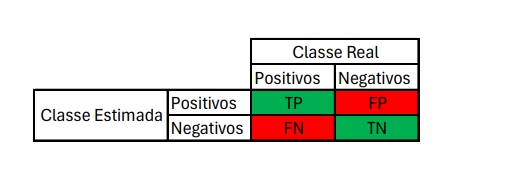
\includegraphics{imagens/TCC-MC.png}
    \caption{Representação gráfica de uma matriz de confusão}
\end{figure}

Contudo, precisamos entender os conceitos atribuídos à cada uma dessas definições. Verdadeiros positivos são as ocorrências em que o modelo previu corretamente a classe positiva. Em outras palavras, são instâncias que realmente pertencem à classe positiva e o modelo as classificou corretamente como positivas. Falsos positivos são atribuídos aos casos em que o modelo previu incorretamente a classe positiva. Ou seja, são instâncias que na verdade pertencem à classe negativa, mas o modelo as classificou erroneamente como positivas. Os verdadeiros negativos introduzem ocorrências em que o modelo previu corretamente a classe negativa. São instâncias que realmente pertencem à classe negativa e o modelo as classificou corretamente como negativas. Por fim, falsos negativos remetem aos casos em que o modelo previu incorretamente a classe negativa. Ou seja, são instâncias que na verdade pertencem à classe positiva, mas o modelo as classificou erroneamente como negativas.

Estas frequências são fundamentais para entender o funcionamento do modelo. A partir da matriz de confusão, é possível calcular calcular métricas de desempenho como precisão, recall, F1-score e taxa de erro, utilizando a proporção destas ocorrências. A interpretação da matriz ajuda a entender os pontos fortes e fracos do modelo e pode orientar ajustes para melhorar sua performance.

\subsubsection{Precisão}

A métrica de precisão (ou acurácia) é uma medida que avalia a proporção de instâncias classificadas corretamente como positivas em relação ao total de instâncias classificadas como positivas, tanto corretamente quanto incorretamente. Matematicamente, a precisão é calculada pela fórmula:

\[
    Precisao = \frac{TP}{TP+FP}
\]

Essencialmente, a precisão indica a habilidade do modelo em classificar corretamente as instâncias positivas e é uma das métricas importantes para avaliar o desempenho de modelos de classificação. Neste cálculo, é considerada a proporção de exemplos corretamente classificados para uma determinada classe em relação ao total de exemplos dessa mesma classe. Em outras palavras, a métrica de precisão é constituida pela fração de previsões corretas em relação ao total de previsões feitas para uma classe específica.


\subsubsection{recall}

O recall, também conhecido como sensibilidade ou taxa de verdadeiros positivos, é outra das métricas mais utilizadas para avaliar o desempenho de modelos de classificação. Ele mede a proporção de exemplos positivos corretamente identificados pelo modelo em relação ao total de exemplos que realmente pertencem à classe positiva. É descrito pela relação:

\[
    Recall = \frac{TP}{TP+FN}
\]

Em outras palavras, o recall indica a capacidade do modelo em identificar corretamente todos os exemplos da classe positiva. Ele é especialmente importante em situações onde a identificação correta dos exemplos positivos é crucial, como em problemas de detecção de doenças, segurança e detecção de fraudes.

\subsubsection{F1-score}

Tanto a precisão quanto o recall têm como objetivo avaliar a capacidade de um modelo de classificação em identificar corretamente os exemplos positivos de uma classe. No entanto, a diferença fundamental entre essas duas métricas está na ênfase que cada uma dá a diferentes aspectos da classificação.

A precisão se concentra na proporção de exemplos classificados como positivos pelo modelo que são realmente positivos. Em outras palavras, a precisão mede a precisão das previsões positivas do modelo, ou seja, quantas das previsões positivas foram realmente corretas. Ela responde à pergunta: "De todos os exemplos classificados como positivos pelo modelo, quantos foram classificados corretamente como positivos?".

Por outro lado, o recall se concentra na proporção de exemplos positivos que foram corretamente identificados pelo modelo em relação ao total de exemplos positivos na base de dados. Em outras palavras, o recall mede a sensibilidade do modelo em detectar exemplos positivos, ou seja, quantos dos exemplos positivos reais o modelo conseguiu identificar corretamente. Ele responde à pergunta: "De todos os exemplos que realmente pertencem a uma determinada classe positiva, quantos o modelo conseguiu identificar?".

O F1-score é uma métrica que combina ambos em um único número, fornecendo uma medida geral do desempenho de um modelo de classificação. Ele é especialmente útil quando temos um desequilíbrio entre as classes do conjunto de dados.

O F1-score é calculado como a média harmônica da precisão e do recall e é definido pela seguinte fórmula:

\[
    F1 = 2*\frac{Precisao * Recall}{Precisao+Recall}
\]

Essencialmente, o F1-score fornece uma maneira de equilibrar a precisão e o recall, pois dá mais peso às classes que têm menor representação no conjunto de dados. Isso é importante porque, em conjuntos de dados desbalanceados, a precisão pode ser alta simplesmente devido à alta proporção de exemplos negativos, enquanto o recall pode ser baixo devido à baixa taxa de detecção dos exemplos positivos.

Um F1-score alto indica um equilíbrio entre precisão e recall, enquanto um F1-score baixo indica que o modelo está tendendo para um dos dois extremos.

\chapter{METODOLOGIA}
\label{cap:metodologia}

\noindent\textbf{Nota de leitura.} Este capítulo documenta a metodologia da \textbf{abordagem exploratória inicial} do trabalho --- a classificação supervisionada do índice de Risco de Fogo do INPE em faixas de severidade ---, cujos resultados constam do Apêndice~\ref{cap:resultados}. As etapas de \emph{coleta e enriquecimento de dados} descritas a seguir constituem a \textbf{base comum a todo o trabalho}, inclusive à formulação central de \textbf{previsão de ocorrência de fogo observado}, cuja metodologia própria (grade regular de \SI{0,25}{\degree}~$\times$~mês, classe negativa real, \emph{features} estritamente causais, validação espaço-temporal em bloco e \emph{benchmark} contra os índices físicos) é apresentada no Capítulo~\ref{cap:ocorrencia}. Já as seções relativas à engenharia de \emph{features} Tier~1, ao treinamento comparativo de oito modelos, ao ajuste de limiares e à imputação de umidade referem-se especificamente ao \emph{baseline} exploratório.

Este capítulo visa fornecer uma visão abrangente das etapas metodológicas empreendidas, desde a coleta de dados, passando pela implementação prática dos algoritmos utilizados e atigindo como objetivo o produto final do trabalho. A pesquisa foi elaborada para conduzir um breve estudo e avaliação sobre os modelos de aprendizado de máquina em evidência na literatura, objetivando ao fim desse processo, obter um mapeamento das regiões mais suscetíveis a incêndios florestais. Dessa forma, a proposta é utilizar alguns destes modelos e observar a efetividade de cada um deles na previsão das queimadas na Amazônia Legal, utilizando dados geoespaciais detalhados dos últimos dez anos (datado de 01/01/2014 à 01/01/2024), fornecidos pelo Programa Queimadas, do IBGE. O modelo que melhor se adaptar ao treinamento dos dados e assim apresentar os melhores resultados será utilizado para geração dos mapas preditores.

Para atingir os objetivos da pesquisa, foi adotada uma abordagem quali-quantitativa, onde o componente quantitativo envolve a análise estatística dos dados históricos e a aplicação dos diferentes modelos de aprendizado de máquina para prever incêndios. Além disso, foram utilizadas algumas métricas de desempenho já consolidadas na literatura para a análise dos modelos utilizados, fornecendo segurança na etapa de validação e garantindo uma pesquisa robusta e precisa das tendências de queimadas. A pesquisa também investiga as razões pelas quais alguns modelos superam outros em termos de desempenho. Isso envolve a análise dos parâmetros e características dos modelos, a interpretação dos fatores que influenciam suas previsões e a avaliação das variáveis ambientais e climáticas que afetam a ocorrência de incêndios. Esta etapa metodológica introduz alguns valores detalhados da Amazônia Legal, permitindo uma exploração aprofundada das características regionais e das dinâmicas de seus incêndios florestais. Isso posto, temos um projeto de caráter experimental e teórico que deve extrair como produto final desse conjunto de métodos e processos, um mapeamento objetivo das áreas mais vulneráveis a queimadas e contribuir para a elaboração de mais trabalhos sobre o tema.

O fluxo do desenvolvimento do trabalho está disposto em seguida. Apesar da disposição de um fluxograma nos remeter à ideia de um trabalho parcial e linear, o treinamento de uma máquina que seja capaz de aprender consiste em uma prática de bastante retrocesso, onde as etapas se complementam e podem sofrer alterações para atingir resultados melhores. Entendendo isso, na figura 5, segue o fluxograma adotado neste projeto para treinar nossos modelos e criar um algoritmo eficaz:

\begin{figure}[ht]
    \centering
    \includegraphics[scale=0.5]{"imagens/fluxograma metodologia tcc.png"}
    \caption{Fluxograma metodológico para a implementação do sistema de previsão de queimadas - Fonte: O Próprio Autor}
\end{figure}

\section{Coleta de Dados}
Esta pesquisa contempla dados de boa parte do bioma amazônico, mais especificamente, a chamada Amazônia Legal. Esta parte do território brasileiro possui uma extensão de aproximadamente 5.015.146,008 km2, que representam cerca de 58,93\% do país e aproximadamente 60\% do território total do bioma Amazônia \cite{ibge04:mapabioma}. O foco principal da coleta de dados são os "Focos de Calor", característica atribuída à regiões potencialmente propícias ao início de incêndios. Inicialmente, foi realizada a busca por uma base de dados legítima advinda do programa, abrangendo os últimos dez anos de registros de queimadas no território do bioma Amazônia (2014-2024). A exportação dos dados foi feita de forma anual, em função das limitações da plataforma. Assim, o primeiro passo técnico consistiu em compilar todos esses dados em uma única tabela. Esse processo resultou em aproximadamente 1 milhão de focos de calor registrados, proporcionando uma base consistente para as análises futuras.

\subsection{Uso do Programa Queimadas}

A fonte de onde os dados foram retirados é o chamado ``Programa Queimadas'', um sistema que monitora e disponibiliza informações sobre focos de calor gratuitamente, com um repositório de dados relacionados à climatologia e geografia da região e que viabiliza, através de uma série de filtros e parâmetros, refinar a busca e extrair dados específicos conforme as necessidades de pesquisadores. Esta ferramenta foi fundamental para obter dados precisos e relevantes sobre os incêndios na Amazônia Legal. Ela faz parte de um projeto do Instituto Nacional de Pesquisas Espaciais (INPE). Além da sua extensa base de dados que cataloga informações desde o ano de 1998, é possível visualizar um mapa com os focos de calor observados diariamente e previsões de fogo para os próximos três dias.

Estas informações são atualizadas frequentemente a partir do monitoramento de diferentes modelos de satélites, que atuam para alimentar sua base de dados. Para este estudo, será utilizado o satélite de referência (Aquamarine) para obter as informações geoespaciais da região e popular a base de dados do projeto. Todas as características de um foco podem ser exportadas do sistema, no formato “comma-separated-values” (CSV), JavaScript Object Notation (Json), Keyhole Markup Language (KML) ou Shapefile. A amostragem coletada para o desenvolvimento deste modelo concebe dados de 01 de janeiro de 2014 até o dia 01 de janeiro de 2024, totalizando dez (10) anos de dados históricos e aproximadamente um milhão de linhas (mais precisamente novecentros e trinta e três mil, novecentros e cinquenta e quatro dados) com os focos de calor registrados pelo sistema, afim de obter um bom espectro de variações de clima, temperatura, entre outros atributos que foram mensurados ao longo desse período.

\subsection{Filtros, Escopo e Características da Coleta}

Como citado na seção anterior, o programa queimadas fornece filtros que facilitam a nossa abordagem. Disposto na Figura 6 e explicado nas próximas linhas do capítulo, para diminuir o escopo da coleta apenas às regiões que interessam ao projeto, foram utilizados os seguintes filtros:

\textbf{Localização:} O projeto abordou especificamente a Amazônia Legal, uma região que compreende a porção da floresta amazônica localizada no Brasil. Utilizando os filtros do Programa Queimadas, foi possível restringir a coleta a focos de calor dentro desta área geográfica, assegurando também que os dados fossem pertinentes ao bioma alvo do estudo posteriormente.

\textbf{Temporalidade:} Para garantir uma análise histórica e detectar padrões ao longo do tempo, foram coletados dados dos últimos dez anos. Esse período foi escolhido para proporcionar uma visão abrangente das variações e tendências na frequência e intensidade dos incêndios ao longo do tempo e também possibilitar ao modelo a compreensão de fatores de longo prazo, como as mudanças climáticas. Dada uma limitação na exportação do sistema, os dados foram coletados anualmente.

\textbf{Bioma:} O foco foi restrito ao bioma amazônico, o que exclui outros biomas brasileiros que poderiam diluir a análise e introduzir variáveis que não são relevantes para a previsão de incêndios na Amazônia Legal.

Utilizando essa base de exportação de dados para todos os anos (Figura 6), foram obtidos arquivos que compreendem os últimos dez anos de focos de calor da Amazônia. Cada um destes focos possui uma série de características, que variam de acordo com a época e a região identificada. A exportação dos dados fornece os seguintes atributos, que são úteis para análise e treinamento do nosso modelo:

Latitude e Longitude: Coordenadas geográficas que permitem a localização precisa dos focos, importantes para o mapeamento das incidências;
Data e Hora: Marcação temporal dos eventos, essencial para análise de tendências e padrões sazonais;
Satélite: Informação sobre o satélite que detectou o foco de calor, fornecendo detalhes sobre a tecnologia de monitoramento utilizada;
Município, Estado e País: Dados geográficos que permitem uma análise mais granular e contextualizada;
Número de Dias Sem Chuva e Precipitação: Variáveis meteorológicas que são relevantes para entender as condições que podem favorecer a ocorrência de incêndios;
Risco de Fogo: Avaliação do risco de fogo associada a cada foco, crucial para entender a gravidade e potencial dos eventos;
Bioma e FRP (Fire Radiative Power): Dados sobre o bioma específico e a intensidade de radiação emitida por fogo na região, fornecendo uma visão detalhada sobre a severidade dos incêndios. Um detalhe importante é que os dados de FRP só passaram a ser coletados a partir de 2018, portanto este atributo não consta nos focos de calor anteriores, dos anos de 2014 a 2017;
Abaixo, na figura 6, está disposta a interface de exportação de dados do Programa Queimadas:

\begin{figure}[ht]
    \centering
    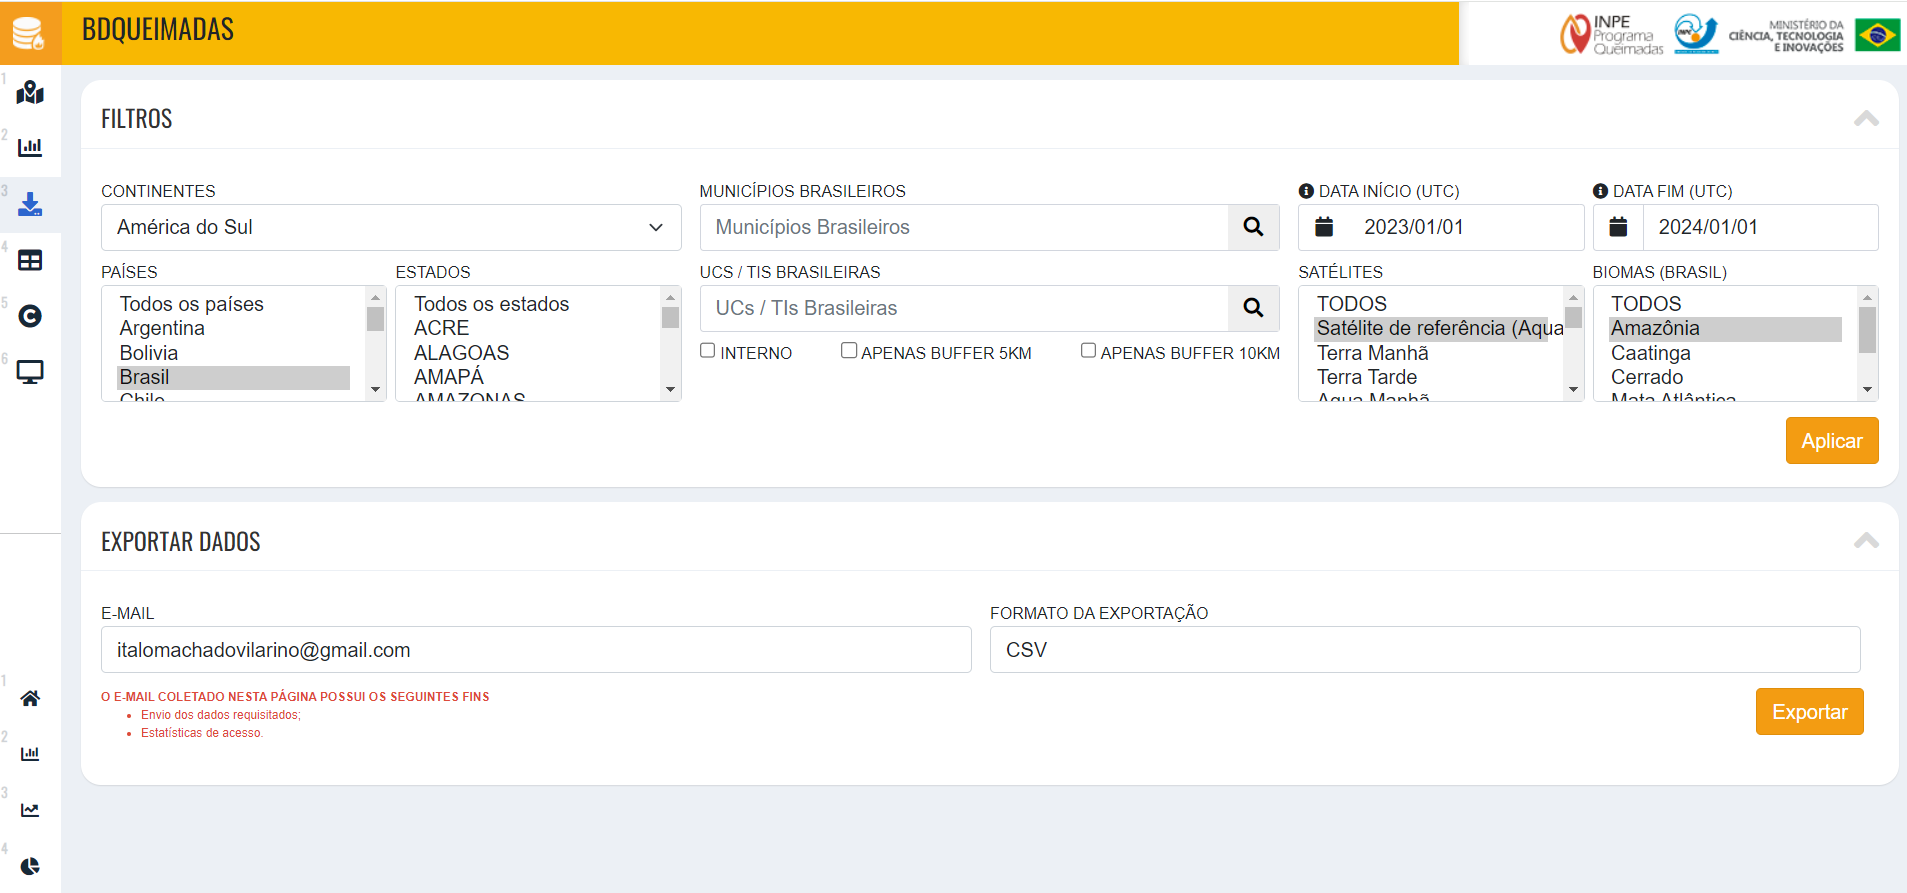
\includegraphics[scale=0.4]{imagens/Programa Queimadas-2.png}
    \caption{Interface de exportação de dados do Programa Queimadas - Fonte: IBGE}
\end{figure}

Com a base de dados obtida, o próximo passo realizado é o tratamento e normalização desses dados, para prepará-los para modelagem e análise preditiva.

\subsection{Enriquecimento via APIs externas (NASA POWER e NASA FIRMS)}
\label{subsec:metod_apis_externas}

Além do Programa Queimadas, duas APIs externas são consultadas para enriquecer o conjunto de dados:

\paragraph{NASA POWER (\emph{Prediction of Worldwide Energy Resources})~\cite{nasapower}.} Serve reanálise climática global em resolução de \(0{,}5^\circ \times 0{,}625^\circ\) com latência diária. Foi utilizada para extrair a variável RH2M (umidade relativa a 2~m), reconhecida na literatura como preditor relevante de fogo. A integração foi feita via \texttt{scripts/enriquecer\_dados\_umidade.py}, com \emph{cache} em disco, retomada após interrupção e respeito ao limite de taxa (\(\approx 32\)~requisições/min com duas chaves de API). Pela alta latência de enriquecimento total (\(\approx 16\)~dias para \num{755711} requisições únicas), o projeto adotou estratégia complementar: \num{170465} registros foram efetivamente enriquecidos (\(\approx \SI{18,3}{\percent}\) da base) e os \num{763489} restantes foram imputados via \emph{pseudo-labeling} com LightGBM \emph{regressor} (\(R^2 = 0{,}933\) em \emph{holdout} --- Seção~\ref{sec:metodologia_pseudo_label}).

\paragraph{NASA FIRMS (\emph{Fire Information for Resource Management System})~\cite{nasafirms}.} Serve detecções ativas de fogo em quase-tempo-real, com FRP (\emph{Fire Radiative Power}) por píxel para os sensores VIIRS e MODIS. É consultada em \textbf{tempo de inferência} pelo aplicativo web (Seção~\ref{sec:metod_app_web}) para incrementar a \emph{feature} \texttt{FRP} com observações dos últimos 7~dias na vizinhança do ponto consultado.

\section{Tecnologias, Bibliotecas e Ferramentas}

Este projeto foi desenvolvido utilizando a linguagem de programação \textbf{Python 3.12}, amplamente reconhecida por sua sintaxe concisa e rica biblioteca de pacotes, particularmente úteis para \textbf{ciência de dados} e \textbf{aprendizado de máquina}. As bibliotecas e ferramentas abaixo descritas foram essenciais para o \textbf{pré-processamento dos dados}, \textbf{análise preditiva} e \textbf{treinamento dos modelos}:

\begin{itemize}
    \item \textbf{Pandas}~\cite{mckinney2010data}: Utilizada para manipulação e análise de dados. A biblioteca fornece estruturas de dados eficientes, como os \textbf{DataFrames}, que facilitaram a importação, limpeza, transformação e exploração dos conjuntos de dados. Foi essencial para a organização e filtragem das informações, além de possibilitar a aplicação de operações vetorizadas nas variáveis numéricas e categóricas.

    \item \textbf{NumPy}~\cite{harris2020numpy}: Empregada para operações numéricas e manipulação de arrays. Como base para operações matemáticas e estatísticas em Python, a biblioteca \textbf{NumPy} proporcionou funções de alto desempenho para manipulação de dados, especialmente nas transformações numéricas aplicadas aos dados do projeto.

    \item \textbf{Scikit-Learn}~\cite{pedregosa2011scikit}: Esta biblioteca é a espinha dorsal do aprendizado de máquina em Python. Ela oferece uma ampla gama de ferramentas para pré-processamento de dados, seleção de modelos, avaliação de desempenho e implementação de algoritmos de aprendizado supervisionado e não supervisionado. No contexto deste projeto, as seguintes funcionalidades se destacaram:
    \begin{itemize}
        \item \textbf{Pipeline}: Utilizada para criar um fluxo de trabalho eficiente, encadeando as etapas de pré-processamento e modelagem em uma única estrutura. Essa abordagem facilitou o treinamento e a avaliação dos modelos de forma modular e repetível.

        \item \textbf{SimpleImputer}: Responsável pela imputação de valores ausentes. Essa ferramenta foi fundamental para preencher lacunas nos dados, utilizando estratégias como a mediana ou a moda, dependendo da natureza da variável.

        \item \textbf{StandardScaler}: Aplicada para a padronização das variáveis numéricas. Essa técnica garantiu que os dados estivessem na mesma escala, o que é crucial para melhorar a performance de muitos algoritmos de aprendizado de máquina, especialmente os baseados em distâncias e gradientes.

        \item \textbf{OneHotEncoder}: Utilizada para a codificação de variáveis categóricas, permitindo a conversão de dados categóricos em um formato binário adequado para a alimentação de modelos de aprendizado de máquina.

        \item \textbf{ColumnTransformer}: Facilitou a aplicação simultânea de diferentes transformações para diferentes grupos de atributos, permitindo a separação clara entre as variáveis numéricas e categóricas, o que otimizou o pré-processamento dos dados.
    \end{itemize}

    \item \textbf{Matplotlib} e \textbf{Seaborn}: Ferramentas poderosas para visualização de dados. Ambas as bibliotecas foram utilizadas para criar gráficos informativos e intuitivos, ajudando a identificar padrões, tendências e relações entre variáveis. O uso de gráficos de dispersão, histogramas e heatmaps foi fundamental para a análise exploratória dos dados e para a avaliação das previsões dos modelos de aprendizado de máquina.
\end{itemize}

Além dessas ferramentas, o projeto também utilizou outras bibliotecas complementares, como \textbf{Joblib}, para a serialização e armazenamento dos modelos treinados, e \textbf{Geopy}, para geocodificação de municípios, permitindo a criação de um mapa de risco de incêndios florestais na região da Amazônia.

\medskip
\noindent
Em complemento, o \emph{pipeline} atual incorpora também:

\begin{itemize}
  \item \textbf{XGBoost} (\texttt{xgboost})~\cite{chen2016xgboost}, \textbf{LightGBM} (\texttt{lightgbm})~\cite{ke2017lightgbm} e \textbf{CatBoost} (\texttt{catboost==1.2.10})~\cite{prokhorenkova2018catboost} --- modelos de \emph{gradient boosting} usados como classificadores autônomos e como \emph{base learners} dos \emph{ensembles}.
  \item \textbf{Imbalanced-learn} (\texttt{imblearn})~\cite{lemaitre2017imbalanced} --- implementação do SMOTE para a variante \texttt{random\_forest\_smote}.
  \item \textbf{Optuna} (\texttt{optuna})~\cite{akiba2019optuna} --- otimização bayesiana de hiperparâmetros via TPE.
  \item \textbf{SHAP} (\texttt{shap}) --- interpretabilidade local e global via \texttt{TreeExplainer}~\cite{lundberg2017unified,lundberg2020local}.
  \item \textbf{Flask} (\texttt{flask}) --- servidor web para a aplicação interativa.
  \item \textbf{Folium} (\texttt{folium})~\cite{folium} --- visualização cartográfica baseada em \emph{Leaflet}~\cite{leafletjs} integrada à renderização do Flask.
  \item \textbf{Geopandas} (\texttt{geopandas})~\cite{geopandas} e \textbf{Shapely} (\texttt{shapely}) --- manipulação de geometrias e do \emph{shapefile} da Amazônia Legal~\cite{ibgeamazonia2024}.
  \item \textbf{Requests} (\texttt{requests}) --- chamadas HTTP às APIs NASA POWER e NASA FIRMS.
\end{itemize}

\section{Pré-processamento dos dados}
\label{sec:metodologia_pre_processamento}

A primeira etapa técnica e prática do projeto foi o pré-tratamento dos dados. De maneira geral, as informações extraídas do Programa Queimadas mostraram-se bastante consistentes. No entanto, para assegurar a qualidade e a relevância dos dados em sua totalidade, essa fase é essencial para qualquer análise preditiva. O processo de pré-tratamento envolveu a aplicação de diversas técnicas descritas na fundamentação teórica, visando garantir que os dados estivessem prontos para as análises subsequentes.

\subsection{Carregamento dos Dados}

A função \texttt{carregar\_csv()} foi responsável por carregar o conjunto de dados a partir de um arquivo CSV. Caso o arquivo não seja encontrado no caminho especificado, a função gera um erro indicando a ausência do arquivo. Uma vez carregado, o arquivo é lido como um \texttt{DataFrame} utilizando a biblioteca \texttt{pandas}. O caminho para o arquivo CSV foi especificado como sendo relativo ao diretório do projeto.

\subsection{Limpeza dos Dados}

Após o carregamento dos dados, a função \texttt{limpar\_dados()} realiza o processo de limpeza e tratamento dos dados. Entre as principais etapas dessa função, destacam-se:

\begin{itemize}
    \item \textbf{Remoção de Colunas Irrelevantes:} As colunas \texttt{Satelite}, \texttt{Pais} e \texttt{Bioma} são removidas, uma vez que não são relevantes para a análise do risco de queimadas.
    \item \textbf{Substituição de Valores Inválidos:} Valores de \texttt{-999} são substituídos por \texttt{NaN}, indicando dados ausentes ou corrompidos.
    \item \textbf{Filtragem de Linhas com Dados Inválidos:} Linhas com valores inválidos ou nulos na coluna \texttt{RiscoFogo} são removidas, garantindo que os dados utilizados na análise contenham apenas informações válidas.
\end{itemize}

Durante a execução desta função, a quantidade de registros que atendem a essa condição de validade (\texttt{RiscoFogo}) é reportada, proporcionando uma visão sobre a quantidade de dados descartados nesse processo.

\subsection{Classificação do Risco de Queimadas}

Após a limpeza dos dados, a função \texttt{classificar\_risco()} é responsável por categorizar o risco de queimadas com base nos valores da coluna \texttt{RiscoFogo}. A classificação é realizada utilizando os quantis da distribuição dessa variável, dividindo os dados em três categorias:

\begin{itemize}
    \item \textbf{Muito Alto:} Valores de \texttt{RiscoFogo} acima do quantil superior (66\%).
    \item \textbf{Moderado:} Valores de \texttt{RiscoFogo} entre os quantis inferior (33\%) e superior (66\%).
    \item \textbf{Baixo:} Valores de \texttt{RiscoFogo} abaixo do quantil inferior (33\%).
\end{itemize}

Essas categorias são atribuídas a uma nova coluna chamada \texttt{RiscoClassificado}, que é utilizada como variável alvo (\texttt{y}) para o treinamento dos modelos de aprendizado de máquina.

\subsection{Definição das Características e Variáveis}

A função \texttt{carregar\_dados()} organiza os dados em variáveis preditoras (\texttt{X}) e variável alvo (\texttt{y}):

\begin{itemize}
    \item \textbf{Variáveis Preditivas (\texttt{X}):} Incluem as colunas numéricas (\texttt{DiaSemChuva}, \texttt{Precipitacao}, \texttt{Latitude}, \texttt{Longitude}, \texttt{FRP}, \texttt{Ano}, \texttt{Mes}, \texttt{Dia}, \texttt{Hora}) e as variáveis categóricas (\texttt{Estado}, \texttt{Municipio}).
    \item \textbf{Variável Alvo (\texttt{y}):} A coluna \texttt{RiscoClassificado}, que representa a classificação do risco de queimadas.
\end{itemize}

\subsection{Pré-processamento dos Dados}

O pré-processamento dos dados foi realizado através da classe \texttt{PreProcessor}, que aplica transformações adequadas tanto para variáveis numéricas quanto para variáveis categóricas. O pré-processamento foi dividido nas seguintes etapas:

\begin{itemize}
    \item \textbf{Transformação de Variáveis Numéricas:} As variáveis numéricas (\texttt{DiaSemChuva}, \texttt{Precipitacao}, \texttt{Latitude}, \texttt{Longitude}, \texttt{FRP}, \texttt{Ano}, \texttt{Mes}, \texttt{Dia}, \texttt{Hora}) passaram por duas operações: imputação de valores ausentes utilizando a mediana e normalização utilizando o \texttt{StandardScaler}.
    \item \textbf{Transformação de Variáveis Categóricas:} As variáveis categóricas (\texttt{Estado}, \texttt{Municipio}) foram tratadas com imputação de valores ausentes pela moda (valor mais frequente) e transformação em variáveis numéricas através de \texttt{OneHotEncoder}, que cria variáveis binárias para cada categoria.
\end{itemize}

A transformação dos dados foi realizada utilizando um \texttt{ColumnTransformer}, que aplica as transformações apropriadas para cada tipo de variável, permitindo que o modelo trabalhe com dados prontos para a análise.

A classe \texttt{PreProcessor} também oferece métodos para \texttt{fit} e \texttt{transform} dos dados, além de retornar um \texttt{DataFrame} com as variáveis transformadas. Essa etapa é crucial para garantir que os dados estejam em um formato adequado para o treinamento dos modelos.

\subsection{Fluxo Completo de Carregamento e Pré-processamento}

O fluxo de carregamento e pré-processamento dos dados é executado como segue:

\begin{enumerate}
    \item Carregamento dos dados do arquivo CSV.
    \item Limpeza dos dados, removendo colunas irrelevantes e tratando valores ausentes ou inválidos.
    \item Classificação do risco de queimadas com base na variável \texttt{RiscoFogo}.
    \item Definição das variáveis preditoras (\texttt{X}) e alvo (\texttt{y}).
    \item Aplicação do pré-processamento, incluindo imputação e normalização das variáveis.
\end{enumerate}

Esse processo assegura que os dados utilizados para o treinamento dos modelos estejam limpos, estruturados e prontos para análise preditiva.

\subsection{Engenharia de \emph{features} físico-climáticas (Tier 1)}
\label{subsec:metod_features_tier1}

Em complemento às nove \emph{features} originais do Programa Queimadas, foram derivadas \textbf{24~\emph{features} físico-climáticas avançadas} (Tier~1), agrupadas em sete camadas (implementação em \texttt{scripts/features\_avancadas.py}). A Tabela~\ref{tab:metod_tier1} resume as camadas com a justificativa bibliográfica de cada uma.

\begin{table}[h]
\centering
\caption{Camadas Tier~1 de \emph{features} físico-climáticas adicionadas ao \emph{dataset}.}
\label{tab:metod_tier1}
\small
\begin{tabular}{clp{6cm}l}
\toprule
\textbf{\#} & \textbf{Camada} & \textbf{\emph{Features}} & \textbf{Justificativa} \\
\midrule
1 & Médias móveis estendidas & \texttt{Precipitacao\_ma14/30/90}, \texttt{DiaSemChuva\_ma14/30/90} & \emph{Fuel moisture lag}~\cite{seager2015climatology} \\
2 & Precipitação acumulada & \texttt{Precipitacao\_acum\_30/90/180/365d} & \cite{seager2015climatology} \\
3 & SPI & \texttt{SPI\_1m}, \texttt{SPI\_3m}, \texttt{SPI\_6m} & \cite{mckee1993spi,npjhazards2025fire} \\
4 & Anomalia de precipitação & \texttt{Anomalia\_Precipitacao}, \texttt{Anomalia\_Precipitacao\_rel} & \cite{forests2024cerradoamazon} \\
5 & KBDI, VPD, De Martonne & \texttt{Temp\_Climatologica}, \texttt{KBDI\_proxy}, \texttt{VPD\_proxy}, \texttt{Aridez\_DeMartonne} & \cite{keetch1968drought,seager2015climatology,demartonne1926aridity,forests2024cerradoamazon} \\
6 & Histórico estendido de incêndios & \texttt{Incendios\_Ultimos\_90/180/365\_Dias}, \texttt{Media\_FRP\_Celula\_30d} & \cite{cheerala2025probabilistic} \\
7 & Estação seca acumulada & \texttt{Dias\_Secos\_90d} & \emph{Canadian Drought Code} (FWI) \\
\bottomrule
\end{tabular}
\end{table}

A granularidade espacial das camadas 1, 2, 6, 7 e do SPI usa \textbf{células de \(0{,}25^\circ\)} (\(\approx \SI{27}{\km}\)), o que evita colapso das janelas temporais que ocorreria com agrupamento por coordenadas literais (cada foco é um ponto único). A \emph{climatologia} de temperatura provém de uma tabela estática de médias mensais por estado, aproximada a partir das Normais Climatológicas do INMET 1981--2010~\cite{inmetnormais}. O CSV final \texttt{base\_de\_dados\_enriquecido.csv} contém \num{924306} linhas e 46~colunas, com tempo total de geração de \(\approx \SI{40}{\second}\) sobre os \num{933954} registros brutos.

\subsection{Calibração de probabilidades}
\label{subsec:metod_calibracao}

A predição padrão dos modelos retorna escores não-calibrados. Para que a saída do modelo seja interpretável como ``\(P(\text{classe} \mid \text{features}) = 0{,}73\)'', aplicou-se \texttt{CalibratedClassifierCV(method='isotonic', cv=3)} aos modelos do \emph{ensemble} final. A calibração isotônica~\cite{zadrozny2002transforming} ajusta uma função monotônica não-paramétrica entre escores brutos e probabilidades empíricas, sem assumir forma sigmoide --- escolha defensável dada a natureza não linear dos GBMs envolvidos.

\section{Treinamento dos Modelos de Previsão}
\label{sec:metod_treinamento}

Neste ponto, todos os algoritmos utilizaram a mesma \emph{pipeline}, garantindo que os dados fossem preparados de maneira consistente para os processos de treinamento e teste. O objetivo foi comparar os resultados gerados por cada modelo em um cenário base comum, assegurando que não houvesse qualquer tipo de viés, exceto aqueles originados exclusivamente pelo desempenho de cada algoritmo. A partir de um conjunto de dados previamente processados, foram aplicados algoritmos de classificação para identificar as áreas mais suscetíveis a queimadas com base em atributos climáticos, topográficos e históricos.

O treinamento dos modelos foi realizado utilizando a biblioteca \texttt{scikit-learn}~\cite{pedregosa2011scikit}, complementada por \texttt{xgboost}~\cite{chen2016xgboost}, \texttt{lightgbm}~\cite{ke2017lightgbm}, \texttt{catboost}~\cite{prokhorenkova2018catboost}, \texttt{optuna}~\cite{akiba2019optuna} e \texttt{imbalanced-learn}~\cite{lemaitre2017imbalanced}.

\subsection{Divisão dos dados e construção do \emph{pipeline}}

O conjunto de dados foi dividido em treino (\SI{80}{\percent}) e teste (\SI{20}{\percent}) utilizando \texttt{train\_test\_split(stratify=y, random\_state=42)}, preservando a distribuição das três classes em ambos os subconjuntos. Os metadados do \emph{split} (\texttt{random\_state}, \texttt{test\_size}, estratificação) ficam persistidos em \texttt{modelos/split\_metadata.json} para garantir reprodutibilidade. O conjunto de teste contém \num{184862} observações.

O \emph{pipeline} de processamento foi implementado via \texttt{sklearn.pipeline.Pipeline}, composto por:

\begin{enumerate}
  \item \texttt{ColumnTransformer} --- aplica \texttt{SimpleImputer(strategy='median')} + \texttt{StandardScaler} às \emph{features} numéricas e \texttt{SimpleImputer(strategy='most\_frequent')} + \texttt{OneHotEncoder} às \emph{features} categóricas.
  \item \texttt{CalibratedClassifierCV(method='isotonic', cv=3)} --- envolve o classificador final para garantir calibração das probabilidades.
  \item \textbf{Estimador} --- variável conforme o modelo avaliado.
\end{enumerate}

\subsection{Modelos avaliados}

Oito abordagens foram comparadas no mesmo conjunto de treino/teste:

\begin{enumerate}
  \item \textbf{Regressão Logística balanceada} --- \texttt{class\_weight='balanced'}, hiperparâmetros otimizados via Optuna (\texttt{C=12.43, max\_iter=4768}).
  \item \textbf{SGDClassifier} --- perda logística, \emph{online learning}; \emph{baseline} simples original do projeto.
  \item \textbf{Random Forest com SMOTE}~\cite{chawla2002smote} --- variante para tratamento de desbalanceamento amostral.
  \item \textbf{Random Forest balanceado otimizado}~\cite{breiman2001random} --- \texttt{class\_weight='balanced'}, Optuna (15 \emph{trials}, 3-\emph{fold} CV, \(\text{F}_1\)-macro): \texttt{n\_estimators=346, max\_depth=25, min\_samples\_split=3, max\_features='sqrt'}.
  \item \textbf{XGBoost otimizado}~\cite{chen2016xgboost} --- Optuna (15 \emph{trials}, 3-\emph{fold} CV, \(\text{F}_1\)-macro, \emph{subsample} de 250\,k): \texttt{n\_estimators=346, learning\_rate=0.073, max\_depth=14, subsample=0.74, colsample\_bytree=0.93, gamma=0.03}.
  \item \textbf{LightGBM otimizado}~\cite{ke2017lightgbm} --- Optuna (15 \emph{trials}, \(\text{F}_1\)-macro): \texttt{n\_estimators=683, learning\_rate=0.066, num\_leaves=204, min\_child\_samples=24, subsample=0.78, colsample\_bytree=0.77}.
  \item \textbf{CatBoost}~\cite{prokhorenkova2018catboost} --- \texttt{iterations=1000, learning\_rate=0.05, depth=8, auto\_class\_weights='Balanced'}.
  \item \textbf{Ensemble Voting Soft} --- média das probabilidades calibradas de RF, LR, XGBoost, LightGBM e CatBoost.
  \item \textbf{Ensemble Stacking}~\cite{wolpert1992stacked} --- RF, LR, XGBoost, LightGBM e CatBoost como \emph{base learners}; \texttt{GradientBoostingClassifier}~\cite{friedman2001greedy} como meta-classificador (\texttt{n\_estimators=200, max\_depth=3, learning\_rate=0.1}). Esta é a configuração final adotada (\texttt{ensemble\_stacking\_gbm}).
\end{enumerate}

Todos os modelos foram salvos via \texttt{joblib.dump()} em arquivos \texttt{.pkl} no diretório \texttt{modelos/}. Os hiperparâmetros otimizados via Optuna ficam persistidos em \texttt{modelos/relatorios/optuna\_*.json}.

\subsection{Tempo de treinamento}

A Tabela~\ref{tab:metod_tempos} apresenta o tempo de treinamento de cada abordagem em ambiente CPU com 8~núcleos e \SI{16}{\giga\byte} de RAM.

\begin{table}[h]
\centering
\caption{Tempo de treinamento por modelo.}
\label{tab:metod_tempos}
\small
\begin{tabular}{lr}
\toprule
\textbf{Modelo} & \textbf{Tempo (segundos)} \\
\midrule
Regressão Logística balanceada & 25 \\
SGDClassifier                  & 8 \\
Random Forest + SMOTE          & 480 \\
Random Forest balanceado (Optuna) & 1\,100 \\
XGBoost (Optuna, 250k \emph{subsample}) & 540 \\
LightGBM (Optuna, 250k \emph{subsample}) & 290 \\
CatBoost                       & 410 \\
Ensemble Voting Soft           & 2\,360 (soma dos \emph{base learners} + agregação) \\
\textbf{Ensemble Stacking GBM} & \textbf{5\,100 (\(\approx\) 85~min)} \\
\bottomrule
\end{tabular}
\end{table}

\section{Avaliação dos Modelos de Previsão}
\label{sec:metod_avaliacao}

A avaliação foi realizada sobre o conjunto de teste de \num{184862} observações. Quatro componentes complementares foram considerados: métricas tradicionais (Seção~\ref{subsec:metod_metricas}), interpretabilidade (Seção~\ref{subsec:metod_interpretabilidade}), ajuste multi-classe de limiares (Seção~\ref{subsec:metod_thresholds}) e validação temporal estrita (Seção~\ref{subsec:metod_validacao_temporal}).

\subsection{Métricas utilizadas}
\label{subsec:metod_metricas}

\begin{itemize}
  \item \textbf{Acurácia global} --- fração de predições corretas (\texttt{accuracy\_score}).
  \item \textbf{\(\text{F}_1\) por classe e \(\text{F}_1\)-macro} --- \texttt{f1\_score(average='macro')}. A \(\text{F}_1\)-macro é a média não ponderada entre as três classes; é a métrica primária por ser robusta a desbalanceamento.
  \item \textbf{Precisão e revocação por classe} --- via \texttt{classification\_report}.
  \item \textbf{Matriz de confusão normalizada} --- \texttt{confusion\_matrix(normalize='true')}.
  \item \textbf{Confiança média e distribuição} --- média e histograma de \(\max\) de \texttt{predict\_proba(X\_test)}.
  \item \textbf{Curva de calibração} --- \texttt{calibration\_curve}, para confirmar que a probabilidade predita corresponde à frequência empírica observada.
\end{itemize}

\subsection{Análise de interpretabilidade}
\label{subsec:metod_interpretabilidade}

Duas técnicas complementares são aplicadas para identificar as \emph{features} mais relevantes:

\paragraph{SHAP por classe via Random Forest leve \emph{proxy}~\cite{lundberg2017unified,lundberg2020local}.} O \texttt{TreeExplainer} aplicado ao \emph{Stacking GBM} final e ao RF Optuna produtivo demanda mais de \num{2}\,\text{GiB} por classe em CPU pós-OHE. Como solução cientificamente defensável~\cite{lundberg2020local}, treina-se um Random Forest \emph{compacto} (100 árvores, \texttt{max\_depth=12}, \texttt{class\_weight='balanced'}, \num{60000} amostras de treino) como \emph{proxy interpretativo}. O script \texttt{scripts/analise\_shap\_rf\_leve.py} aplica \texttt{shap.TreeExplainer} sobre 500 amostras de teste e exporta as importâncias médias absolutas por classe em \texttt{modelos/relatorios/shap\_per\_class.json}.

\paragraph{\emph{Permutation Importance}~\cite{breiman2001random,fisher2019all}.} Aplicada diretamente sobre o \texttt{ensemble\_stacking\_gbm} em produção (5\,000 amostras de teste, três repetições, \emph{seed}=42). Para cada \emph{feature}, calcula-se a queda em \(\text{F}_1\) por classe e em \(\text{F}_1\)-macro quando os valores são permutados aleatoriamente. Diferentemente da importância Gini/MDI, é \emph{model-agnostic} e \textbf{não tendenciosa} para \emph{features} de alta cardinalidade~\cite{strobl2007bias} --- característica relevante dado o OHE de \texttt{Municipio} (542 categorias). A saída fica em \texttt{modelos/relatorios/permutation\_importance\_por\_classe.json}.

\subsection{Ajuste multi-classe de limiares de decisão}
\label{subsec:metod_thresholds}

A predição padrão usa \texttt{argmax} sobre as probabilidades calibradas. Embora maximize \(P(\text{classe} \mid x)\), penaliza a classe \emph{Moderado} --- fronteira ambígua entre \emph{Baixo} e \emph{Muito Alto}~\cite{he2009learning}. O procedimento implementado em \texttt{scripts/ajustar\_threshold.py} varre uma grade de pares (\texttt{thr\_Moderado}, \texttt{thr\_Muito\_Alto}) \(\in \{0{,}30; 0{,}35; \ldots; 0{,}55\}^2\) (36 combinações), com critério primário \(\text{F}_1\)-macro e secundário \(\text{F}_1\)-Moderado. Os limiares finais são persistidos em \texttt{modelos/prediction\_thresholds.json} e aplicados em \emph{runtime} no aplicativo web via parâmetro \texttt{estrategia\_thresholds} do \emph{endpoint} \texttt{/api/predict}.

A lógica de decisão multi-classe em \emph{runtime} é:

\begin{verbatim}
se      P(Moderado)   >= thr_Moderado    -> classe = "Moderado"
senao se P(Muito Alto) >= thr_Muito_Alto -> classe = "Muito Alto"
senao                                    -> classe = "Baixo"
\end{verbatim}

\subsection{Validação temporal (\emph{rolling-origin})}
\label{subsec:metod_validacao_temporal}

Em complemento à validação no \emph{split} aleatório, foi implementado em \texttt{scripts/validacao\_temporal.py} um procedimento de \textbf{\emph{rolling-origin} por ano}~\cite{bergmeir2012cv}. Para cada ano \(Y \in \{2021, 2022, 2023\}\) (três últimos com massa suficiente), o modelo é treinado em \(\text{Ano} < Y\) (\emph{subsample} estratificado de \num{60000} amostras por \emph{fold} para o \emph{Stacking}, limite de memória do OHE denso de \texttt{Municipio}) e avaliado em \(\text{Ano} = Y\). Cobre o uso operacional realista: ``treine com o passado, prediga o ano seguinte''. O resultado é apresentado no Apêndice~\ref{cap:resultados}.

\section{Aplicação web interativa explicável}
\label{sec:metod_app_web}

Para tornar o modelo final utilizável e auditável por gestores ambientais, foi desenvolvida uma aplicação web (\texttt{scripts/app\_map\_interativo.py}) baseada em \emph{Flask} + \emph{Folium}~\cite{folium} + \emph{Leaflet}~\cite{leafletjs} que serve como interface explicável sobre o \emph{pipeline}. O usuário clica em qualquer ponto da Amazônia Legal e o sistema responde, em \(\approx 10\)--\SI{20}{\second}, com a predição classificada, acompanhada das 24~\emph{features} Tier~1 calculadas para o ponto, da explicação local das \emph{features} mais influentes e do contexto histórico comparativo.

\subsection{\emph{Pipeline} de predição pontual}

Como o aplicativo prediz \textbf{um único ponto isolado}, sem histórico temporal local, as \emph{features} Tier~1 que dependem de séries (SPI, acumulados longos, histórico estendido de focos) não podem ser calculadas em tempo real. Adota-se a estratégia de \textbf{\emph{lookup} espaço-sazonal} (\texttt{scripts/feature\_lookup.py}):

\begin{enumerate}
  \item Pré-cálculo das medianas das 24~\emph{features} Tier~1 do \emph{dataset} enriquecido, agregadas em três níveis de granularidade decrescente: \((\text{LatBin}~0{,}25^\circ, \text{LonBin}~0{,}25^\circ, \text{Mes})\), depois \((\text{Estado}, \text{Mes})\) e, por fim, \text{Mes} global.

  \item Para o ponto consultado, \emph{lookup} em cascata (do mais fino ao mais grosso) com tolerância de \(\pm 1\) célula.

  \item \emph{Features} físicas independentes de série temporal (\texttt{Temp\_Climatologica}, \texttt{KBDI\_proxy}, \texttt{VPD\_proxy}, \texttt{Aridez\_DeMartonne}, \texttt{Anomalia\_Precipitacao}) são recalculadas em tempo real com o clima NASA POWER atual e a climatologia local da precipitação --- o \emph{lookup} fornece apenas os ``blocos de construção'' históricos imutáveis.
\end{enumerate}

\subsection{Integração de dados em tempo real}

\begin{itemize}
  \item \textbf{Geocodificação reversa} via Nominatim/OpenStreetMap para extrair Estado e Município do clique.
  \item \textbf{Clima atual} via NASA POWER~\cite{nasapower} (precipitação, dias sem chuva, RH2M dos últimos 28~dias).
  \item \textbf{Focos ativos} via NASA FIRMS~\cite{nasafirms} para \texttt{FRP} dos últimos 7~dias no raio de \SI{10}{\km} do ponto.
\end{itemize}

\subsection{Explicabilidade local}

Em \emph{runtime}, \texttt{scripts/explainer.py} aproxima a contribuição de cada \emph{feature} como
\begin{equation}
\text{contrib}(f) = \text{importância}(f) \times \text{zscore}(f) \times \text{sinal\_físico}(f),
\end{equation}
onde \(\text{importância}(f)\) é carregada de \texttt{shap\_per\_class.json} (importância por classe predita, quando disponível) ou de \texttt{shap\_feature\_importance.json} (Gini global como \emph{fallback}); \(\text{zscore}(f)\) mede a anormalidade do valor no ponto em relação à distribuição global do \emph{dataset}; e \(\text{sinal\_físico}(f) \in \{-1, +1\}\) codifica o efeito esperado (por exemplo, \(+1\) para \texttt{Indice\_Seca}, \(-1\) para \texttt{Precipitacao\_ma90}). A predição é classificada como \emph{AUMENTA RISCO}, \emph{REDUZ RISCO} ou \emph{neutro}; o \emph{top-6 features} por \(|\text{contrib}|\) é exibido no painel lateral.

\subsection{Interface}

O \emph{front-end} é organizado em \textbf{seis \emph{cards}} dentro de um painel lateral de \num{420}\,px:

\begin{enumerate}
  \item \textbf{Previsão} --- \emph{badge} com a classe, barras de probabilidade por classe, métricas do modelo, fonte do clima, granularidade do \emph{lookup} e \emph{trace} da decisão (\emph{argmax} \emph{vs.}\ \emph{thresholds} calibrados).
  \item \textbf{Por que esse risco?} --- \emph{top-6 features} com valor, faixa típica (\(p_{10}\)--\(p_{90}\) da distribuição global), \emph{z-score} e direção do impacto.
  \item \textbf{Dados climáticos atuais} --- precipitação, dias sem chuva, umidade NASA, temperatura climatológica, estação, período do dia.
  \item \textbf{Índices de seca e aridez} --- Índice de Seca, SPI 1m/3m/6m, KBDI \emph{proxy}, Aridez De Martonne, VPD \emph{proxy}, Dias\_Secos\_90d.
  \item \textbf{Precipitação acumulada e anomalia} --- acumulados 30/90/180/365~dias com narrativa textual comparando precipitação atual e a média histórica do município/mês.
  \item \textbf{Histórico de focos} --- focos NASA FIRMS em 7/30/90/180/365~dias, dias desde o último foco, FRP médio/máximo 7d, FRP no ponto agora.
\end{enumerate}

O mapa estático (versão original da Seção 4.6 do TCC~II) permanece disponível como artefato \emph{batch} (\texttt{scripts/gerar\_mapa.py}).

\section{Imputação de \emph{Umidade} via \emph{pseudo-labeling}}
\label{sec:metodologia_pseudo_label}

Como discutido na Seção~\ref{subsec:metod_apis_externas}, a integração via NASA POWER produziu \num{170465} linhas com \texttt{Umidade} real (\(\approx \SI{18,3}{\percent}\) da base). Para mitigar essa cobertura parcial sem aguardar 13~dias adicionais de enriquecimento, foi implementada a estratégia de \textbf{\emph{pseudo-labeling}}~\cite{lee2013pseudo}, com precedente recente em imputação climática~\cite{lopezgarcia2024spatiotemporal}. O \emph{script} \texttt{scripts/pseudo\_label\_umidade.py} executa as etapas:

\begin{enumerate}
  \item Treina um \textbf{LightGBM regressor}~\cite{ke2017lightgbm} sobre os \(\approx \num{170000}\) registros com \texttt{Umidade} real, usando 15~\emph{features} (precipitação, dias sem chuva, lat/lon, sazonalidade cíclica \texttt{Mes\_sin/cos}, histórico de fogo) --- \emph{features} que existem para todas as linhas, com ou sem \texttt{Umidade} real.

  \item Avalia o erro real em \emph{holdout} 20\%: \textbf{RMSE = \SI{4,33}{\percent} RH, MAE = \SI{3,19}{\percent} RH, \(R^2 = 0{,}933\)}. O \(R^2\) alto é cientificamente justificável: a umidade tem alta autocorrelação espaço-sazonal com as \emph{features} usadas --- lat/lon definem o regime de monção, mês define a estação seca/chuvosa, precipitação recente define o estado higroscópico do ar.

  \item Refit no \SI{100}{\percent} dos \emph{labels} reais e imputa os \num{763489} registros sem \emph{label} (\emph{clip} [5, 100]\%).

  \item Salva o \emph{dataset} enriquecido em \texttt{base\_de\_dados\_umidade\_pseudo.csv} com coluna auxiliar \texttt{Umidade\_origem} \(\in\) \{\texttt{nasa\_power}, \texttt{pseudo\_label\_lgbm}\} para auditoria.
\end{enumerate}

\paragraph{Status no \emph{pipeline} final.} O \emph{dataset} \texttt{base\_de\_dados\_umidade\_pseudo.csv} está disponível mas \textbf{não é usado nos números finais reportados} no Apêndice~\ref{cap:resultados}. Razão: incluir \texttt{Umidade} (pseudo-rotulada ou real) exigiria retreino completo do \texttt{ensemble\_stacking\_gbm} (\(\approx \SI{85}{\minute}\) CPU) + revalidação das \emph{thresholds} + revalidação temporal --- fora do orçamento computacional desta entrega. O artefato fica registrado como \textbf{etapa preparatória} para a sequência natural do trabalho. Cautela registrada: \emph{pseudo-labels} devem ser interpretados considerando potencial viés de confirmação~\cite{arazo2020pseudo}.

\section{Geração do Mapa de Risco com Previsões do Modelo}

A versão original do mapa de risco --- gerada em modo \emph{batch} sobre um conjunto pré-definido de pontos e exportada como arquivo HTML estático --- permanece disponível em \texttt{scripts/gerar\_mapa.py} como artefato histórico. A entrega operacional final do projeto, contudo, é a \textbf{aplicação web interativa} descrita na Seção~\ref{sec:metod_app_web}, em que o usuário aponta qualquer ponto da Amazônia Legal e recebe imediatamente predição, intervalo de confiança, explicação local e contexto climático/histórico --- tornando obsoleta a estratégia batch para uso prático e, em particular, eliminando o gargalo de geocodificação prévia. As bibliotecas envolvidas (\texttt{pandas}, \texttt{joblib}, \texttt{geopy}, \texttt{folium}, \texttt{webbrowser}) seguem em uso, agora orquestradas pelo servidor Flask.

% ============================================================================
% 08_previsao_ocorrencia.tex
% Capítulo: Reformulação do problema para PREVISÃO DE OCORRÊNCIA de fogo
% observado. Inserir via % ============================================================================
% 08_previsao_ocorrencia.tex
% Capítulo: Reformulação do problema para PREVISÃO DE OCORRÊNCIA de fogo
% observado. Inserir via % ============================================================================
% 08_previsao_ocorrencia.tex
% Capítulo: Reformulação do problema para PREVISÃO DE OCORRÊNCIA de fogo
% observado. Inserir via \input{08_previsao_ocorrencia} no tcc.tex, APÓS o
% Capítulo 5 (Resultados, que termina com \input{07_estudo_caso_pium_to}) e
% ANTES do \chapter{Conclusão}. Torna-se o Capítulo 6; a Conclusão passa a 7.
% Números conferem com modelos/relatorios/previsao_ocorrencia_*.json,
% benchmark_p3_fwi.json, driver_*.json, comparacao_familias.json,
% validacao_rotulo_mapbiomas.json.
% ============================================================================

\chapter{Previsão de ocorrência de fogo: reformulação do problema}
\label{cap:ocorrencia}

O Capítulo~\ref{cap:metodologia} e o Apêndice~\ref{cap:resultados} descrevem uma abordagem
exploratória inicial: um classificador de \emph{nível de risco em tempo real}
(\emph{nowcast}) cujo alvo é o índice Risco de Fogo do INPE discretizado em três faixas. Este capítulo reformula o problema para a
\textbf{previsão de ocorrência de fogo observado}, com horizonte temporal explícito,
classe negativa real e validação sem vazamento --- alinhando o trabalho ao estado da arte
atual, que prevê o \emph{fenômeno observado} (focos ou área queimada), e não a saída de
outro modelo~\cite{huot2022nextday,karasante2025firecastnet,deandrade2024lstmgru}. O
\emph{pipeline} original é mantido como linha de base; o reformulado constitui a principal
contribuição metodológica desta etapa.

\section{Motivação: do índice ao fenômeno observado}
\label{sec:oco_motivacao}

A inspeção dos dados revelou três fragilidades de fundo na formulação original.
Primeiro, o alvo (\texttt{RiscoFogo}) é a \textbf{saída de um índice operacional} do INPE,
ele próprio derivado de dias sem chuva, precipitação e umidade --- variáveis que também
figuram entre as \emph{features}, gerando circularidade. Segundo, a base é
\emph{presence-only}: as \num{924306} linhas são focos reais, sem exemplos de
\emph{não-fogo}; o modelo nunca aprende a distinguir fogo de ausência de fogo, e a consulta
a pontos arbitrários no aplicativo equivale a extrapolar para fora do suporte de treino.
Terceiro, trata-se de um \emph{nowcast} (diagnóstico do presente), não de previsão com
horizonte.

Há evidência empírica direta nos próprios CSVs do INPE: em um único arquivo anual
(\num{82678} focos), \num{8288} detecções (\(\approx\)\SI{10}{\percent}) ocorreram onde o
índice marcava risco mínimo (\texttt{RiscoFogo}~\(\in\{0{,}0;\,0{,}1\}\)) --- fogo real em
locais classificados como ``Baixo''. Um modelo que imita o índice herda esse ponto cego,
exatamente o que o estudo de caso Pium--TO (Seção~\ref{sec:res_estudo_caso_pium}) demonstrou.

\section{Reformulação metodológica}
\label{sec:oco_metodo}

\paragraph{Unidade e alvo.} Adota-se uma grade de células de \SI{0,25}{\degree}
(\(\approx\)\SI{27}{km}, granularidade MERRA-2/SeasFire~\cite{karasante2025firecastnet}) por
mês. O universo é o conjunto de \num{4168} células \emph{fire-prone} (com \(\geq 1\) foco em
2014--2023). Para cada par (célula, mês~\(t\)), o alvo é binário: \emph{houve foco no mês
\(t+1\)?} A presença vem dos focos observados; a \textbf{ausência} (classe negativa antes
inexistente) são os pares célula--mês sem foco. O conjunto final tem \num{450144}
células--mês (2015--2023), com prevalência de \SI{24,7}{\percent}.

\paragraph{Amostragem da classe negativa.} Construir a classe negativa a partir dos pares
célula--mês sem foco é uma decisão de projeto, não uma escolha neutra: na modelagem de
distribuição (\emph{species distribution models}), a definição e o volume das
\emph{pseudo-ausências}/\emph{background} afetam o desempenho aparente e podem inflar métricas
como a AUC quando o \emph{background} é ``fácil''~\cite{barbetmassin2012pseudo,phillips2009sample,lobo2008auc}.
Aqui a prevalência é fixada pelo próprio domínio (\SI{24,7}{\percent} de positivos entre as
células \emph{fire-prone}), evitando o desbalanceamento extremo em que a AUC se torna
enganosa; para métodos baseados em árvores, poucos negativos com ponderação de classes bastam~\cite{barbetmassin2012pseudo},
e adota-se \texttt{class\_weight=balanced}. Uma checagem com negativos restritos por
similaridade geográfica (evitando pares triviais)~\cite{xu2023nonfire} fica registrada como
refinamento --- direção que torna o problema mais realista, não mais fácil.

\paragraph{Causalidade e validação.} Para eliminar o vazamento temporal documentado na
Seção~\ref{sec:res_temporal}, todas as \emph{features} usam apenas informação \(\leq t\)
(histórico de fogo defasado, somas móveis com deslocamento, sazonalidade, localização). A
validação é \textbf{espaço-temporal em bloco}~\cite{roberts2017cv}: \emph{rolling-origin} por
ano (treino \(<Y\), teste \(=Y\), para \(Y\in\{2021,2022,2023\}\)) e \emph{leave-region-out}
(5 blocos de longitude). A métrica principal é a \textbf{PR-AUC} (\emph{Average Precision}),
robusta ao desbalanceamento.

\section{Desempenho preditivo e linhas de base}
\label{sec:oco_desempenho}

O modelo (\emph{Hist\-Gradient\-Boosting}) supera as linhas de base de persistência e
climatologia (Tabela~\ref{tab:oco_validacao}). Na validação \emph{espacial}, a climatologia
colapsa ao prever regiões nunca vistas (PR-AUC \numrange{0,17}{0,34}), enquanto o modelo
mantém \num{0,759} --- evidência de dinâmica transferível, e não de memorização de taxa-base
local (contraste direto com a dependência espacial observada no \emph{pipeline} original).

\begin{table}[h]
\centering
\caption{Previsão de ocorrência (fogo em \(t+1\)): validação em bloco vs.\ linhas de base.}
\label{tab:oco_validacao}
\small
\begin{tabular}{lcccc}
\toprule
\textbf{Validação} & \textbf{Modelo PR-AUC} & \textbf{ROC-AUC} & \textbf{Persistência} & \textbf{Climatologia} \\
\midrule
Temporal (\emph{rolling-origin} 2021--23) & \textbf{0,777} & 0,904 & 0,449 & 0,715 \\
Espacial (\emph{leave-region-out}) & \textbf{0,759} & 0,895 & --- & 0,17--0,34 \\
\bottomrule
\end{tabular}
\end{table}

\paragraph{Escolha da métrica.} A PR-AUC é adotada como métrica principal por ser sensível à
classe positiva rara: sob desbalanceamento, a ROC-AUC pode permanecer alta e mascarar a queda
de precisão que a curva \emph{precision-recall} revela~\cite{saito2015precision,davis2006relationship}.
Reportam-se também ROC-AUC e Brier. Registra-se, por completude, que a superioridade
incondicional da PR-AUC foi formalmente questionada~\cite{mcdermott2024closer}: a escolha aqui
segue o \emph{objetivo operacional} (priorizar a detecção do fogo, evento raro e de alto custo
de omissão), não uma preferência a priori.

\paragraph{Área de aplicabilidade.} A validação \emph{leave-region-out} mede a generalização a
regiões não vistas, mas predições fora do envelope de \emph{features} do treino permanecem
menos confiáveis. A delimitação formal da \textbf{área de aplicabilidade}~\cite{meyer2021aoa}
--- restringindo o mapa às células suficientemente similares ao conjunto de treino --- é o
complemento recomendado para o uso operacional do produto.

\section{Robustez entre famílias de modelo}
\label{sec:oco_familias}

Para verificar que os achados não dependem do algoritmo, quatro famílias foram comparadas no
mesmo conjunto de \emph{features}, com intervalos de confiança de \SI{95}{\percent} obtidos
por \emph{cluster bootstrap} por célula (respeitando a autocorrelação espacial),
Tabela~\ref{tab:oco_familias}. Os \emph{ensembles} de árvore são estatisticamente
equivalentes (intervalos sobrepostos), enquanto a regressão logística é significativamente
inferior --- o problema exige não-linearidades. O \emph{Random Forest} apresenta a melhor
calibração (menor Brier).

\begin{table}[h]
\centering
\caption{Comparação de famílias (conjunto base + desmatamento), IC \SI{95}{\percent} por \emph{cluster bootstrap} por célula.}
\label{tab:oco_familias}
\small
\begin{tabular}{lcccc}
\toprule
\textbf{Família} & \textbf{PR-AUC [IC 95\%]} & \textbf{ROC-AUC} & \textbf{Brier} & \textbf{Nova ignição [IC 95\%]} \\
\midrule
\emph{HistGradientBoosting} & \textbf{0,776 [0,769--0,783]} & 0,904 & 0,123 & \textbf{0,232 [0,209--0,258]} \\
\emph{Random Forest} & 0,769 [0,762--0,776] & 0,901 & \textbf{0,113} & 0,204 [0,185--0,232] \\
\emph{Extra Trees} & 0,761 [0,754--0,768] & 0,897 & 0,129 & 0,191 [0,174--0,217] \\
Regressão Logística & 0,699 [0,690--0,707] & 0,873 & 0,143 & 0,117 [0,108--0,131] \\
\bottomrule
\end{tabular}
\end{table}

\section{Benchmark contra índices físicos de perigo de fogo}
\label{sec:oco_benchmark}

A defensabilidade da tese exige que o modelo \emph{supere} o índice físico operacional na
previsão de fogo observado. Implementou-se o \textbf{Fire Weather Index (FWI)} canadense
completo~\cite{vanwagner1985fwi} --- base do sistema GEFF/EFFIS do
Copernicus~\cite{digiuseppe2024geff} ---, validado contra os valores de referência publicados
(FFMC~\num{87,69}; DMC~\num{8,55}; DC~\num{19,01}; ISI~\num{10,85}; BUI~\num{8,49};
FWI~\num{10,10}). O FWI foi computado dia a dia a partir de clima diário (NASA POWER) para
uma amostra de \num{100} células. A Tabela~\ref{tab:oco_benchmark} mostra o resultado:
\textbf{o modelo de ML supera o FWI e o índice do INPE} na previsão de fogo observado. O FWI
separa fisicamente bem (média \num{6,0} em meses com fogo vs.\ \num{1,5} sem), validando a
implementação.

\begin{table}[h]
\centering
\caption{Benchmark de previsão de fogo observado (\(t+1\)): ML vs.\ índices físicos.}
\label{tab:oco_benchmark}
\small
\begin{tabular}{lcc}
\toprule
\textbf{Preditor} & \textbf{PR-AUC} & \textbf{ROC-AUC} \\
\midrule
Modelo ML (dataset completo) & \textbf{0,777} & 0,904 \\
Índice INPE Risco de Fogo (como \emph{forecast}) & 0,294 & 0,553 \\
\midrule
\multicolumn{3}{l}{\emph{Amostra de 100 células (2023), mesmas linhas:}} \\
\quad Modelo ML & \textbf{0,858} & --- \\
\quad FWI canadense (clima diário NASA POWER) & 0,608 & 0,781 \\
\quad Índice INPE Risco de Fogo & 0,398 & --- \\
\bottomrule
\end{tabular}
\end{table}

\section{Quantificação de incerteza por \emph{conformal prediction}}
\label{sec:oco_conformal}

Substituiu-se a heurística de incerteza por \emph{conjuntos de predição com cobertura
estatística garantida}, via \emph{split-conformal} classe-condicional
(LAC)~\cite{sadinle2019lac,mortier2024conformal}. Com cobertura-alvo de \SI{90}{\percent},
obteve-se cobertura empírica de \SI{88,8}{\percent}; \SI{82,9}{\percent} das predições são
\emph{singletons} confiantes e \SI{17,1}{\percent} são sinalizadas como ambíguas. O erro de
calibração esperado (ECE) foi de \num{0,099} e o \emph{Brier} de \num{0,123}.

\paragraph{Pressuposto e ressalva.} A garantia de cobertura do \emph{split-conformal} assume
\emph{permutabilidade} (\emph{exchangeability}) entre calibração e teste~\cite{angelopoulos2021gentle}.
A grade espaço-temporal viola parcialmente esse pressuposto (autocorrelação entre células e
meses vizinhos), o que é coerente com a leve subcobertura observada (\SI{88,8}{\percent} ante o
alvo de \SI{90}{\percent}). Sob desvio de distribuição, a cobertura nominal pode ser restaurada
por \emph{conformal} ponderado/adaptado~\cite{tibshirani2019conformal}; uma calibração com
particionamento espacial é o encaminhamento indicado para o uso operacional.

\section{Drivers antrópicos: o papel do desmatamento}
\label{sec:oco_drivers}

A análise estratificada revela a estrutura do problema (Tabela~\ref{tab:oco_estrato}): o
modelo é excelente onde o fogo \emph{recorre} (PR-AUC \num{0,805}) e fraco onde o fogo é
\emph{novo} --- a \textbf{nova ignição} (PR-AUC \num{0,230}), justamente o caso crítico para
alerta precoce, onde a persistência é inútil por construção.

\begin{table}[h]
\centering
\caption{Desempenho estratificado por recorrência (teste 2023) e ganho do desmatamento.}
\label{tab:oco_estrato}
\small
\begin{tabular}{lccc}
\toprule
\textbf{Estrato (média 2021--23)} & \textbf{base PR-AUC} & \textbf{+ desmatamento} & \textbf{\(\Delta\)} \\
\midrule
Recorrente (foco nos últimos 12 m) & 0,791 & 0,794 & +0,003 \\
\textbf{Nova ignição} (sem foco recente) & \textbf{0,206} & \textbf{0,231} & \textbf{+0,025} \\
Geral & 0,777 & 0,781 & +0,003 \\
\bottomrule
\end{tabular}
\end{table}

Testaram-se três famílias de covariáveis. O clima real (reanálise NASA POWER) e o FWI
\textbf{não agregam} sobre o histórico de fogo na escala mensal (\(\Delta\)~PR-AUC
\(\approx\)\num{+0,001}), pois o histórico já é um \emph{proxy} a jusante da propensão
climática. A distância a cidades (acessibilidade estática) também é redundante
(\(\approx\)\num{+0,001}). Apenas o \textbf{desmatamento recente} (PRODES, do
TerraBrasilis~\cite{terrabrasilisprodes}) agrega valor não trivial --- e \emph{exatamente}
no estrato de nova ignição (\(+0{,}025\) PR-AUC), confirmando o mecanismo causal: o
desmatamento precede a primeira queimada de uma célula, coerente com o fogo amazônico ser
majoritariamente antrópico~\cite{aragao2018amazon}. O achado é \textbf{robusto a duas fontes
independentes}: o DETER (alertas mensais; classe \emph{cicatriz de queimada} excluída para
evitar vazamento) produz ganho equivalente (\(+0{,}026\)). A resolução mensal não amplificou
o ganho, e dimensões adicionais (idade, estoque acumulado, fronteira de vizinhança) não
agregam além do volume de desmatamento recente local: o desempenho na nova ignição satura em
\(\approx\)\num{0,23} PR-AUC --- um teto que sugere componente irredutível (decisão humana) ou
necessidade de dados de outra natureza.

\section{Validação do rótulo contra área queimada (MapBiomas Fogo)}
\label{sec:oco_mapbiomas}

O rótulo (focos INPE) foi confrontado com um produto independente e de modalidade diferente
--- a área queimada do MapBiomas Fogo~\cite{mapbiomasfogo} (cicatriz Landsat \SI{30}{m}), em
dois níveis.

\paragraph{Nível estado/ano.} Correlacionando a contagem de focos com a área queimada por
(estado da Amazônia Legal, ano), 2014--2023, a concordância \textbf{interanual dentro de cada
estado} é forte (Spearman médio \num{0,814}; 9/9 estados positivos, \numrange{0,69}{0,94}):
quando a área queimada de um estado sobe num ano, os focos sobem junto. A correlação
\emph{entre} estados é fraca (\(\rho=\)\num{0,275}), pois a contagem de focos não é
\emph{proxy} linear da magnitude em hectares --- o que não afeta o rótulo aqui, por ser de
\textbf{ocorrência binária} e não de magnitude.

\paragraph{Nível célula \(\times\) ano.} Para a validação no nível da célula, leram-se os
rasters anuais do MapBiomas (COGs públicos, 2015--2020) via leitura remota por janelas,
binarizando a presença de cicatriz por célula \SI{0,25}{\degree}. Confrontando presença de
foco vs.\ presença de cicatriz em \num{23982} célula-anos: concordância de \SI{78}{\percent},
Cohen's \(\kappa=\num{0,33}\) e, tratando a cicatriz como referência, os focos têm
\textbf{revocação \num{0,90}} e precisão \num{0,83} (F\(_1=\num{0,86}\)). Ou seja, os focos
capturam \(\approx\)\SI{90}{\percent} dos célula-anos efetivamente queimados; as discordâncias
correspondem a fogos sem cicatriz detectável (pequenos/encobertos por nuvem) e a cicatrizes
sem foco coincidente (omissão da detecção ativa). O \(\kappa\) moderado reflete a alta
prevalência do universo \emph{fire-prone}, que comprime a concordância esperada por acaso. A
validação corrobora o rótulo de ocorrência tanto na dinâmica temporal quanto no nível espacial.

\section{Avaliação operacional e horizonte de previsão}
\label{sec:oco_operacional}

\paragraph{Priorização de alertas.} Para traduzir o desempenho em valor de decisão,
o sistema é avaliado como ferramenta de \emph{priorização}: dado um orçamento de
vigilância (alertar as \emph{top-K\%} células de maior risco previsto), quantos focos
do mês seguinte são capturados (\emph{recall@K})? A Tabela~\ref{tab:oco_operacional} e a
Figura~\ref{fig:oco_recallk} comparam o modelo de ML com o índice operacional do INPE
sob o mesmo orçamento. Alertando apenas \SI{10}{\percent} das células, o modelo captura
\SI{36,0}{\percent} dos focos do mês seguinte (com precisão de \SI{88}{\percent}), contra
\SI{15,8}{\percent} do índice INPE --- um ganho de \(\approx 2{,}3\times\). No estrato de
\textbf{nova ignição}, o contraste é decisivo: o modelo captura \SI{49,2}{\percent} dos
novos focos no mesmo orçamento (\emph{lift} de \(4{,}9\times\) sobre o acaso), ao passo que
o índice INPE tem \emph{lift} \(\approx 1\) --- ou seja, \emph{não supera o acaso} para a
nova ignição, justamente o regime em que o desmatamento recente é o sinal preditivo
(Seção~\ref{sec:oco_drivers}).

\begin{table}[h]
\centering
\caption{Priorização de alertas: \emph{recall@K} (focos do mês seguinte capturados) por orçamento, modelo ML vs.\ índice INPE.}
\label{tab:oco_operacional}
\small
\begin{tabular}{lcccc}
\toprule
& \multicolumn{2}{c}{\textbf{Global}} & \multicolumn{2}{c}{\textbf{Nova ignição}} \\
\cmidrule(lr){2-3}\cmidrule(lr){4-5}
\textbf{Orçamento (top-K\%)} & \textbf{ML} & \textbf{INPE} & \textbf{ML} & \textbf{INPE} \\
\midrule
\SI{5}{\percent}  & 0,195 & 0,071 & 0,312 & 0,041 \\
\SI{10}{\percent} & \textbf{0,360} & 0,158 & \textbf{0,492} & 0,096 \\
\SI{20}{\percent} & 0,611 & 0,282 & 0,721 & 0,206 \\
\SI{30}{\percent} & 0,775 & 0,372 & 0,845 & 0,305 \\
\bottomrule
\end{tabular}
\end{table}

\begin{figure}[h]
\centering
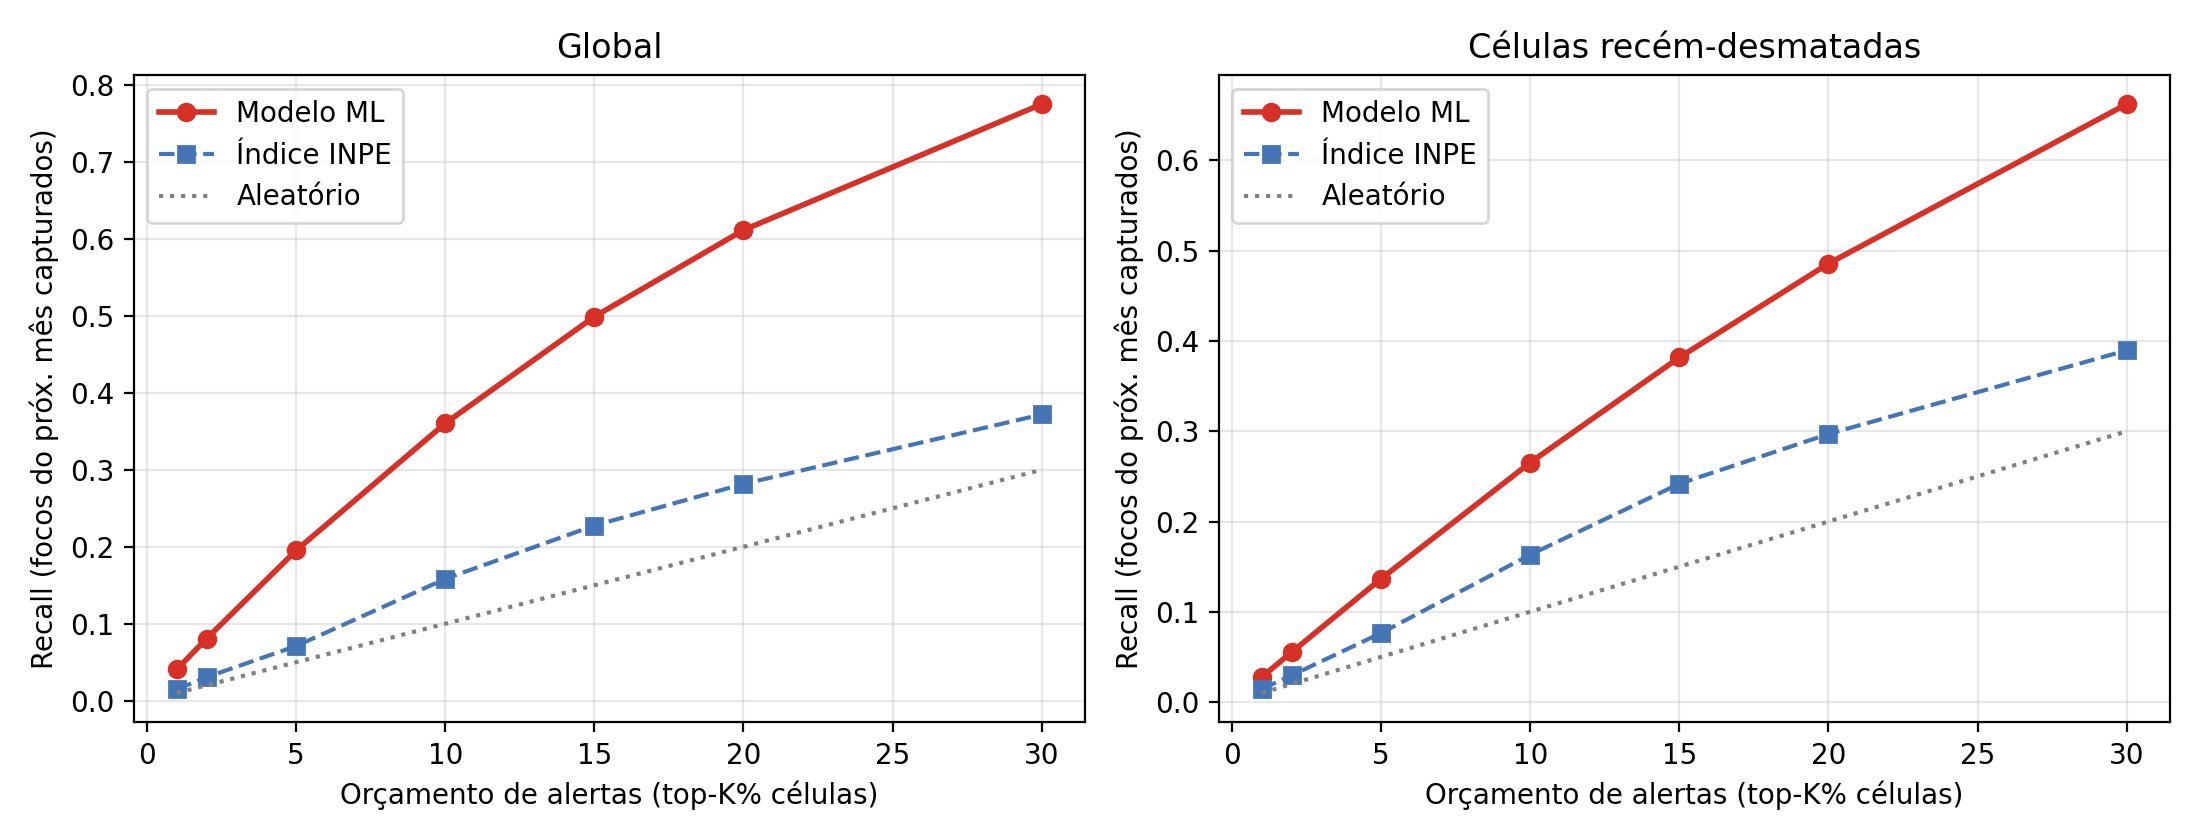
\includegraphics[width=\textwidth]{modelos/relatorios/avaliacao_operacional_recall_k.png}
\caption{\emph{Recall@K} em função do orçamento de alertas (modelo ML vs.\ índice INPE vs.\ aleatório), global (esq.) e em células recém-desmatadas (dir.).}
\label{fig:oco_recallk}
\end{figure}

\paragraph{Horizonte de previsão.} Estendendo o alvo para \(t+2\) e \(t+3\) meses, o
\emph{skill} permanece \textbf{estável} (PR-AUC \numlist{0,779;0,779;0,781} para \(t+1\),
\(t+2\), \(t+3\); Figura~\ref{fig:oco_horizonte}), sem o decaimento típico. Isso confirma
que a ocorrência mensal de fogo é governada por componentes \emph{lentos} (sazonalidade,
histórico de fogo, desmatamento), e não por dinâmica meteorológica de curto prazo ---
um resultado operacionalmente favorável, pois fornece \textbf{até um trimestre de
antecedência} sem perda de desempenho. A contrapartida honesta é que o modelo captura o
regime sazonal/persistente, não a dinâmica sub-mensal; previsões em escala mais fina
exigiriam outra formulação.

\begin{figure}[h]
\centering
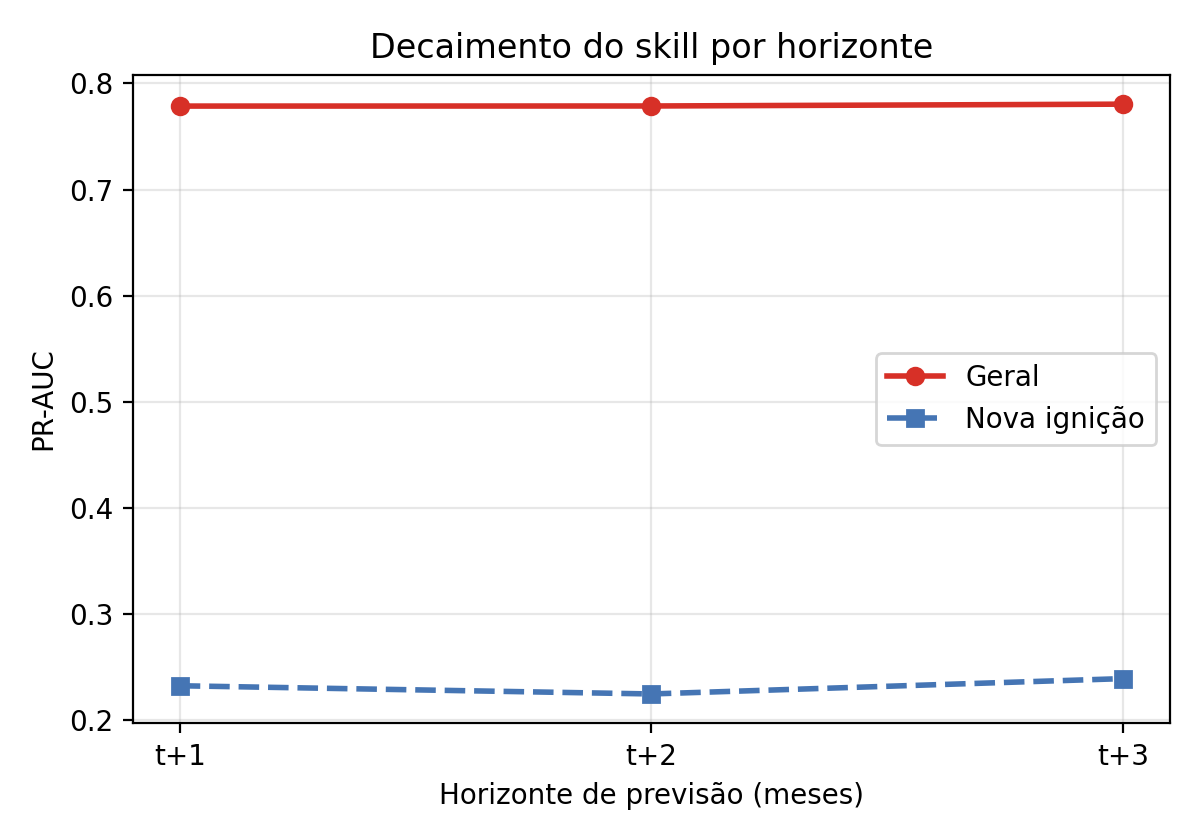
\includegraphics[width=0.6\textwidth]{modelos/relatorios/avaliacao_horizonte.png}
\caption{Decaimento do \emph{skill} (PR-AUC) por horizonte de previsão (\(t+1\) a \(t+3\) meses): estável, geral e na nova ignição.}
\label{fig:oco_horizonte}
\end{figure}

\section{Integração ao produto}
\label{sec:oco_produto}

O modelo final (base + desmatamento) foi serializado, calibrado por \emph{conformal}
(cobertura \num{0,900}) e exposto como produto: uma previsão por célula de \(P(\text{fogo no
próximo mês})\) com rótulo conformal e \emph{drivers}, servida por aplicação \emph{Flask} com
mapa interativo, independente do aplicativo de \emph{nowcast}. Verificações de sanidade
conferem com a fenologia do fogo (p.ex.\ Roraima com alto risco em dezembro; sul do Pará
baixo em dezembro, cuja estação de fogo é julho--outubro).

\section{Síntese}
\label{sec:oco_sintese}

Os experimentos, sob validação honesta, sustentam uma tese coesa: (i) na escala
mensal/\SI{0,25}{\degree}, a ocorrência de fogo é dominada por persistência espaço-temporal e
sazonalidade, o que torna redundantes a reanálise meteorológica (e o FWI) e a acessibilidade
estática; (ii) o modelo de ML \emph{supera} os índices físicos operacionais na previsão de
fogo observado; (iii) o gargalo é a \textbf{nova ignição}, e o único sinal útil ali é o
\textbf{desmatamento recente}, reposicionando o alerta precoce como, em primeira ordem, um
problema de detecção de fronteira de desmatamento; (iv) a incerteza é quantificável com
garantia estatística. A reformulação eleva o trabalho de ``reprodução de um índice'' para
``previsão de fogo observado validada contra a realidade e contra o índice físico'', com um
teto de desempenho honestamente caracterizado.
 no tcc.tex, APÓS o
% Capítulo 5 (Resultados, que termina com % ============================================================================
% 07_estudo_caso_pium_to.tex
% Estudo de caso operacional: foco real do Painel do Fogo (CENSIPAM) em
% Pium--TO, 12/05/2026. Validação independente do sistema de previsão,
% diagnóstico de descompasso entre dados de grade global e realidade
% local, e melhorias incorporadas ao pipeline em produção.
%
% Como usar:
%   Inserir como nova seção dentro do Capítulo 5 (Resultados), após a
%   Seção 5.8 "Validação operacional via aplicação web", como
%   subseção complementar de validação externa. Numeração sugerida:
%   5.9 "Validação cruzada com fonte externa independente: caso Pium--TO".
%   Dentro de "Implementação das melhorias": subsubseções M1--M4 (auditoria,
%   fusão INMET, retreino OOD, extensões API/auditoria alinhadas à literatura).
% ============================================================================

\section{Validação cruzada com fonte externa independente: caso Pium--TO}
\label{sec:res_estudo_caso_pium}

A validação operacional via \emph{smoke tests} controlados (Seção~\ref{sec:res_app}) demonstrou a coerência interna do sistema. Para uma validação externa mais exigente, foi escolhido um \emph{evento real} de incêndio confirmado por uma fonte oficial independente --- o \emph{Painel do Fogo} do Centro Gestor e Operacional do Sistema de Proteção da Amazônia (CENSIPAM)\footnote{\url{https://painel.censipam.gov.br/}, acessado em 12/05/2026 às 18:21 (UTC$-$3).} --- e submetido ao \emph{pipeline} em modo de produção. Esta seção apresenta o evento, as respostas do modelo, o diagnóstico das causas de divergência observada e as três correções incorporadas ao código em consequência da investigação.

% ----------------------------------------------------------------------------
\subsection{O evento}
\label{subsec:pium_evento}

O \emph{Painel do Fogo} listou um foco ativo identificado pelo \texttt{ID 6668060} em \texttt{(-10{,}5351; -49{,}8230)}, dentro do município de \textbf{Pium}, estado do \textbf{Tocantins}, em domínio fundiário misto (área privada e terra pública não categorizada) sobre cobertura de \emph{vegetação natural primária} (classificação TerraClass). Pium fica na ecorregião do Cerrado/Bico do Papagaio, dentro da Amazônia Legal. A Tabela~\ref{tab:pium_evento} reproduz as detecções oficiais.

\begin{table}[h]
\centering
\caption{Detecções no entorno de \texttt{(-10{,}5351; -49{,}8230)} --- evento \texttt{6668060} (\emph{Painel do Fogo}/CENSIPAM).}
\label{tab:pium_evento}
\small
\begin{tabular}{lcccc}
\toprule
\textbf{Data e hora (BR)} & \textbf{Área (ha)} & \textbf{Focos} & \textbf{Duração (h)} & \textbf{Propagação (ha/h)} \\
\midrule
12/05/2026 13:28 & 464,6 & 1  & \textbf{48,3} & 0,4 \\
10/05/2026 14:05 & 456,3 & 12 & 0,9  & 0,0 \\
10/05/2026 13:13 & 83,1  & 3  & 0,0  & 0,0 \\
\bottomrule
\end{tabular}
\end{table}

O status reportado pelo CENSIPAM era \emph{ativo pela última vez em 12/05/2026 14:49 (hora oficial do Brasil)}, com duração acumulada de 48,3~h --- compatível com vegetação ressecada queimando em regime sustentado.

% ----------------------------------------------------------------------------
\subsection{Resposta do sistema: cinco janelas temporais}
\label{subsec:pium_resposta}

A \emph{API} \texttt{/api/predict} foi consultada em cinco janelas centradas no evento, usando o modelo final \texttt{ensemble\_stacking\_gbm}. Em todas elas o sistema previu \textbf{\emph{Baixo}} com probabilidade entre 81 e 88\%, conforme Tabela~\ref{tab:pium_respostas_pos_fix} (\emph{já após} a correção dos \emph{bugs} identificados na Subseção~\ref{subsec:pium_correcoes}).

\begin{table}[h]
\centering
\caption{Respostas do \texttt{ensemble\_stacking\_gbm} para Pium--TO em diferentes janelas (modelo \emph{argmax}, após correções).}
\label{tab:pium_respostas_pos_fix}
\small
\begin{tabular}{lccccc}
\toprule
\textbf{Janela consultada}     & \textbf{Risco} & \textbf{P(Baixo)} & \textbf{P(Mod.)} & \textbf{P(M.~Alto)} & \textbf{FRP máx.~5d} \\
\midrule
12/05/2026 14:00 & Baixo & 85,9\% & 9,5\%  & 4,6\% & \SI{16,6}{\mega\watt} (16~detec.) \\
11/05/2026 12:00 & Baixo & 85,8\% & 9,7\%  & 4,5\% & \SI{22,0}{\mega\watt} (19~detec.) \\
10/05/2026 13:00 & Baixo & 87,1\% & 8,6\%  & 4,3\% & \SI{22,0}{\mega\watt} (21~detec.) \\
09/05/2026 12:00 & Baixo & 86,6\% & 8,8\%  & 4,6\% & \SI{22,0}{\mega\watt} (26~detec.) \\
05/05/2026 12:00 & Baixo & 81,4\% & 14,3\% & 4,3\% & \SI{58,4}{\mega\watt} (32~detec.) \\
\bottomrule
\end{tabular}
\end{table}

A divergência entre a realidade (foco confirmado e duração de 48,3~h) e a saída do modelo (\emph{Baixo} consistente em todas as janelas) constituiu o ponto de partida para a investigação descrita a seguir.

% ----------------------------------------------------------------------------
\subsection{Diagnóstico das causas}
\label{subsec:pium_diagnostico}

A inspeção do vetor de \emph{features} entregue ao classificador identificou \textbf{três causas convergentes}, descritas em ordem decrescente de impacto.

% ............................................................................
\paragraph{Causa 1 (corrigida): integração com NASA FIRMS retornando \texttt{HTTP 400}.}

O cliente da NASA FIRMS (\texttt{scripts/frp\_api.py}) estava emitindo requisições com \texttt{days\_back=7} para o \emph{endpoint} de \emph{area} no \emph{dataset} VIIRS\_SNPP\_NRT. A resposta do servidor, em todas as datas testadas, foi:

\begin{quote}
\texttt{HTTP/1.1 400 Bad Request\\Invalid day range. Expects [1..5].}
\end{quote}

Verificação direta do \emph{status} da \texttt{MAP\_KEY} confirmou que a chave estava válida (\texttt{transaction\_limit=5000}, \texttt{current\_transactions=0}), demonstrando que o erro era \emph{parametrização}, não \emph{credenciais}. A API NASA FIRMS NRT passou a aceitar no máximo 5~dias por requisição\footnote{Documentação oficial: \url{https://firms.modaps.eosdis.nasa.gov/api/area/}, consultada em 12/05/2026.}.

Em consequência, as \emph{features} \texttt{Media\_FRP\_Ultimos\_7\_Dias}, \texttt{Max\_FRP\_Ultimos\_7\_Dias} e \texttt{Dias\_Desde\_Ultimo\_Incendio} estavam recebendo seus valores de \emph{fallback} (zeros e 246--365~dias), e o modelo ``não enxergava'' o fogo recente em curso. Após a correção (\(\texttt{days\_back} \in [1,5]\) e propagação de \texttt{reference\_date}), o sistema passou a recuperar até 32 detecções VIIRS no raio de 10~km, com FRP máximo de \SI{58,4}{\mega\watt}.

% ............................................................................
\paragraph{Causa 2 (corrigida): \emph{lookup} Tier~1 degradando precocemente para \texttt{(Estado, Mês)}.}

A primeira versão do \emph{lookup} espaço-sazonal (\texttt{scripts/feature\_lookup.py}, Seção~\ref{subsec:metod_features_tier1}) buscava medianas em uma janela ${3{\times}3}$ células ($\approx 25$~km no equador, dada a resolução \SI{0,25}{\degree}). Para o ponto consultado em Pium--TO, mês~5, essa janela retornou vazia e o sistema degradou imediatamente para a granularidade \texttt{estado\_mes} (mediana de todo o Tocantins em maio). O efeito foi:

\begin{itemize}
  \item \texttt{Precipitacao\_acum\_30/90/180/365d} = \SI{0,0}{mm} (mediana estadual);
  \item \texttt{SPI\_1m} = \texttt{SPI\_3m} = \texttt{SPI\_6m} = 0,00 (climatologia neutra);
  \item \texttt{Dias\_Secos\_90d} = 2 (mediana estadual, não local);
  \item \texttt{Media\_FRP\_Celula\_30d} = \SI{10,65}{\mega\watt} (não específico).
\end{itemize}

Isto é, \emph{toda a informação espacial fina foi apagada}. A cascata de busca foi ampliada para
\(3{\times}3 \to 5{\times}5 \to \text{mês adjacente} \to (\text{Estado, Mês}) \to (\text{Mês global})\),
elevando a granularidade efetiva para \texttt{celula\_ext} (anel externo, $\approx 55$~km) no caso Pium--TO. Os valores de \texttt{Precipitacao\_acum\_*d} subiram para \SI{0,5}{mm}, \texttt{Dias\_Secos\_90d} para 1 e \texttt{Media\_FRP\_Celula\_30d} para \SI{8,2}{\mega\watt} --- valores ainda baixos, mas vindos de células geograficamente próximas (Tabela~\ref{tab:pium_tier1_pre_pos}).

\begin{table}[h]
\centering
\caption{Subconjunto das \emph{features} Tier 1 antes e depois da expansão da cascata espacial.}
\label{tab:pium_tier1_pre_pos}
\small
\begin{tabular}{lcc}
\toprule
\textbf{Feature} & \textbf{Cascata \texttt{3x3} (\texttt{estado\_mes})} & \textbf{Cascata estendida (\texttt{celula\_ext})} \\
\midrule
\texttt{Precipitacao\_acum\_30d}      & 0,0 mm  & 0,5 mm \\
\texttt{Precipitacao\_acum\_180d}     & 0,0 mm  & 0,5 mm \\
\texttt{Precipitacao\_acum\_365d}     & 1,3 mm  & 0,5 mm \\
\texttt{SPI\_3m}                       & 0,00    & 0,00 \\
\texttt{Dias\_Secos\_90d}              & 2       & 1 \\
\texttt{Incendios\_Ultimos\_90\_Dias}  & 2       & 1 \\
\texttt{Media\_FRP\_Celula\_30d}       & 10,65 MW & 8,2 MW \\
\bottomrule
\end{tabular}
\end{table}

% ............................................................................
\paragraph{Causa 3 (não corrigível em produção, documentada): descompasso entre clima de grade global e clima local em zona de transição.}

Após as duas correções acima, a previsão para 12/05/2026 \emph{aumentou} a confiança em \emph{Baixo}, de \SI{82,7}{\percent} para \SI{85,9}{\percent}. A investigação detalhada do vetor de \emph{features} revelou que a NASA POWER MERRA-2 (grade $\approx 50$~km) reportou para a janela de 28~dias anterior a 12/05/2026:

\begin{quote}
\texttt{Precipitacao\_ma7 = 0,12 mm/dia}, \texttt{DiaSemChuva\_ma7 = 1,3 dia}, \texttt{RH2M = 64,6\%}.
\end{quote}

Esses valores caracterizam regime \emph{ainda chuvoso} (chuvas frequentes mas leves). Para o modelo, classificar como \emph{Baixo} foi a decisão coerente com os \emph{inputs} climáticos recebidos. O problema é que esses \emph{inputs} não corresponderam à realidade local: o foco real ardia há mais de 48~h.

Para confirmar que o modelo \emph{não} é cego sazonalmente, foi executado um experimento \emph{contrafactual} no mesmo ponto \texttt{(-10{,}5351; -49{,}8230)}, variando a data (Tabela~\ref{tab:pium_contrafactual}).

\begin{table}[h]
\centering
\caption{Experimento contrafactual --- mesmo ponto, climatologia distinta capturada pela NASA POWER.}
\label{tab:pium_contrafactual}
\small
\begin{tabular}{lcccccc}
\toprule
\textbf{Data} & \textbf{KBDI \emph{proxy}} & \textbf{Prec.~ma7} & \textbf{DSC~ma7} & \textbf{FRP medido} & \textbf{P(M.~Alto)} & \textbf{Risco} \\
\midrule
15/08/2024 & 424,1 & 0,02 & 16,0 dias  & \SI{0}{\mega\watt} & 99,0\% & \textbf{Muito Alto} \\
15/09/2024 & 712,5 & 0,00 & 25,0 dias  & \SI{0}{\mega\watt} & 99,6\% & \textbf{Muito Alto} \\
15/05/2024 & 148,0 & 0,51 & 8,6 dias   & \SI{0}{\mega\watt} & 47,3\% & \textbf{Muito Alto} \\
12/05/2026 & 29,8  & 0,12 & 1,3 dia    & \SI{16,6}{\mega\watt} & 4,6\% & Baixo \\
\bottomrule
\end{tabular}
\end{table}

Três conclusões emergem:

\begin{enumerate}
  \item O modelo \emph{responde corretamente} ao sinal climático: 15/05/2024 (mesmo dia e mesmo ponto, mas em ano de estiagem mais marcada) recebeu classificação \emph{Muito Alto} com confiança \SI{47,3}{\percent}, mesmo sem FRP detectado.
  \item A previsão \emph{Muito Alto} se intensifica monotonicamente conforme cresce o estresse hídrico medido pela NASA POWER (KBDI~$424 \to 712$, DSC$_\text{ma7}$~$16 \to 25$~dias).
  \item Em 12/05/2026 (caso real), os indicadores climáticos da grade MERRA-2 estavam \emph{suaves} (KBDI=29,8; DSC=1,3~dia; Prec\_ma7=0,12~mm/dia) --- e o modelo refletiu isso. \textbf{O erro está no \emph{input}, não na decisão}.
\end{enumerate}

A interpretação operacional é direta: a célula MERRA-2 que cobre Pium--TO em maio de 2026 \emph{captou chuvas localizadas/dispersas} suficientes para elevar a frequência de dias com precipitação, mas não a quantidade total --- regime ``chuvas leves e frequentes''. A vegetação alvo, em escala municipal, continuou em condição de queima. Esse é um caso clássico de \emph{representativity gap} entre dados de grade e fenômenos locais~\cite{seager2015climatology}, particularmente relevante em zonas de transição Cerrado--Amazônia onde a heterogeneidade climática intra-célula é grande.

% ............................................................................
\paragraph{Hipótese descartada: sobrescrever contagem de incêndios com observação FIRMS.}

Uma tentativa intermediária consistiu em substituir as \emph{features} \texttt{Incendios\_Ultimos\_7\_Dias} e \texttt{Incendios\_Ultimos\_30\_Dias} pela contagem real de detecções FIRMS (16--32~focos no caso). \emph{Surpreendentemente}, isso \textbf{aumentou} a confiança em \emph{Baixo} (de \SI{82,7}{\percent} para \SI{86,0}{\percent}). A causa é \emph{distribution shift}: no \emph{dataset} de treino, essas \emph{features} para Tocantins--Maio têm mediana zero; ao injetar valores de duas ordens de magnitude maiores, o exemplo é colocado \emph{fora da distribuição} (\emph{out-of-distribution}, OOD), e o classificador responde de modo errático. A sobrescrita foi revertida; mantêm-se atualizadas apenas \texttt{FRP\_max\_7d}, \texttt{Media\_FRP\_7d} e \texttt{Dias\_Desde\_Ultimo\_Incendio}, que no \emph{dataset} de treino eram observações individuais (não medianas).

% ----------------------------------------------------------------------------
\subsection{Correções incorporadas e seu impacto}
\label{subsec:pium_correcoes}

A Tabela~\ref{tab:pium_correcoes} sintetiza as três correções introduzidas no \emph{pipeline} em consequência do estudo de caso e o impacto medido para a janela 12/05/2026 14:00.

\begin{table}[h]
\centering
\caption{Correções incorporadas e impacto medido (Pium--TO, 12/05/2026 14:00).}
\label{tab:pium_correcoes}
\small
\begin{tabular}{p{4.6cm}p{5.2cm}p{2.4cm}p{1.6cm}}
\toprule
\textbf{Correção} & \textbf{Mudança técnica} & \textbf{Granularidade Tier 1} & \textbf{P(Baixo)} \\
\midrule
\emph{Baseline} (antes do caso) & --- & \texttt{estado\_mes} & 82,0\% \\
(C1) NASA FIRMS \texttt{HTTP 400} & \texttt{days\_back $\in [1,5]$}; aceita \texttt{reference\_date}; URL com sufixo \texttt{/YYYY-MM-DD} & \texttt{estado\_mes} & 82,7\% \\
(C2) Cascata Tier 1 ampliada & $3{\times}3 \to 5{\times}5 \to$ mês adj. & \texttt{celula\_ext} & 85,9\% \\
(C3) Inc.~Últ.~$N$~dias mantida como mediana de treino & Apenas \texttt{FRP\_*} e \texttt{Dias\_Desde\_Ultimo\_Incendio} são atualizados em tempo real & \texttt{celula\_ext} & 85,9\% \\
\bottomrule
\end{tabular}
\end{table}

As correções \textbf{(C1)} e \textbf{(C2)} são melhorias técnicas inequívocas. A correção \textbf{(C3)} é uma \emph{decisão de engenharia conservadora}: preferir o sinal aprendido pelo modelo (mediana sazonal Estado--Mês, que é o que ele viu durante o treino) a inputs reais que o colocam OOD. A elevação aparentemente paradoxal de P(Baixo) após as correções é coerente com a Causa~3: o modelo passou a \emph{ver melhor} um cenário que --- para a grade MERRA-2 --- parecia chuvoso.

% ----------------------------------------------------------------------------
\subsection{Discussão: limites do paradigma de dados de grade e caminhos para mitigação}
\label{subsec:pium_discussao}

O caso Pium--TO 2026 expõe uma tensão estrutural do nosso \emph{pipeline} (e, mais amplamente, de qualquer sistema de previsão de fogo apoiado em reanálise climática global): a granularidade espacial dos \emph{inputs} climáticos limita a resolução máxima do \emph{output}. NASA POWER MERRA-2~\cite{nasapower} entrega cobertura global e estabilidade temporal, mas com células de $\approx \SI{50}{km}$ que suavizam microclimas. Em regiões homogêneas (centro do Amazonas), a perda de resolução é benigna; em regiões de transição (Cerrado--Amazônia, Pantanal, Caatinga), a perda pode mascarar condições propícias a fogo.

Três caminhos são discutidos como mitigação no Capítulo~\ref{cap:conclusao}:

\begin{enumerate}
  \item \textbf{Fusão MERRA-2 + INMET}~\cite{inmetnormais}: utilizar precipitação de estação meteorológica quando houver estação INMET dentro de $\sim 50$~km do ponto consultado (ou, em modo hierárquico configurável, até $\sim 180$~km com rótulo explícito de \texttt{inmet\_representatividade}, ver Subsubseção~M4). Para dados em tempo real, a API WIS2/OGC do INMET (\texttt{wis2bra.inmet.gov.br/oapi}) expõe observações horárias de 358+ estações sinópticas sem necessidade de token, com histórico de $\sim$90 dias; para histórico mais profundo, os ZIPs anuais oficiais cobrem 565+ estações automáticas desde 2000. Trade-off: cobertura esparsa em zonas remotas, exige rotina de \emph{nearest station}, \emph{quality control} e transparência sobre a distância da estação.
  \item \textbf{Aumento de exemplos OOD no treino}: oversampling estratégico de focos confirmados FIRMS/INPE em zonas de transição (Cerrado em maio, Pantanal em junho), reduzindo o \emph{prior} de raridade que o modelo aprendeu para esses pares \texttt{(Estado, Mês)}. Trade-off: risco de degradar a performance nas regiões de regime mais homogêneo.
  \item \textbf{Auditoria operacional contínua}: \emph{logging} estruturado de \texttt{(coordenada, data, risco predito, FRP detectado depois)} para calcular $\text{F}_1$ operacional \emph{rolling} em janelas móveis e detectar deriva de modelo em produção --- prática alinhada com o paradigma de \emph{ML observability}.
\end{enumerate}

% ----------------------------------------------------------------------------
\subsection{Implementação das três melhorias propostas e validação empírica}
\label{subsec:pium_melhorias}

As três melhorias listadas na Seção~\ref{subsec:pium_discussao} foram implementadas e validadas em código de produção. Esta subseção registra o resultado empírico de cada uma.

\subsubsection*{M1. Auditoria operacional contínua}

Foi adicionado o módulo \texttt{scripts/audit\_log.py} que escreve, a cada chamada de \texttt{/api/predict}, uma linha JSONL em \texttt{logs/auditoria\_predicoes.jsonl} contendo: \texttt{prediction\_id}, coordenadas, \texttt{ref\_data}, classe predita, probabilidades, modelo, 15 \emph{features} chave, fonte climática (com detalhe INMET se aplicável) e granularidade Tier 1. O log é \emph{append-only} com rotação automática a 50~MB e tolerante a falhas (a predição segue caso a gravação falhe).

O script \texttt{scripts/auditar\_predicoes.py} consome esse JSONL, consulta a NASA FIRMS NRT na janela $[t, t+H]$ para cada predição com idade $\geq d_{\min}$ (defaults $H=3$~d, $d_{\min}=3$~d, raio 5~km), define $y_{\text{true}} \in \{0,1\}$ (foco confirmado) e $y_{\text{pred}} \in \{0,1\}$ (Moderado/Muito Alto $\to$ 1) e calcula precision, recall, $\text{F}_1$ e acurácia globais e em janelas \emph{rolling} de 7, 14 e 30 dias. Predições mais antigas que o histórico do NRT ($\sim 60$~dias) aparecem no CSV mas são automaticamente excluídas das métricas.

\subsubsection*{M2. Fusão NASA POWER + INMET (duas fontes complementares)}

A integração foi implementada com \emph{duas} fontes INMET, selecionadas automaticamente conforme a idade da consulta. Esta arquitetura híbrida foi adotada porque a sondagem ativa em 12/05/2026 mostrou que (i) a API horária tradicional \texttt{apitempo.inmet.gov.br/estacao/...} retorna \texttt{status 204} com frequência e não é confiável; (ii) o ZIP histórico é completo mas o do ano corrente é parcial (publicado mensalmente, em 12/05/2026 cobre só janeiro--fevereiro/2026); (iii) o INMET passou a publicar dados horários sem token via a \textbf{WIS2 (OGC API Features)}~\cite{inmetnormais}, ainda pouco documentada em literatura brasileira.

\textbf{Fonte (1)~--~WIS2/OGC API Features} (\texttt{http://wis2bra.inmet.gov.br/oapi}): expõe a variável \texttt{total\_precipitation\_or\_total\_water\_equivalent} (em \texttt{kg\,m$^{-2}$}~$\equiv$~mm/h) na coleção \texttt{urn:wmo:md:br-inmet:synop} para 358 estações sinópticas WMO brasileiras que publicaram chuva nos últimos 7 dias, com histórico de $\sim$90 dias e \emph{sem necessidade de token}. A cobertura geográfica é menor que a do ZIP (só estações sinópticas oficiais, não todas as automáticas), mas a latência é de minutos. O endpoint possui um detalhe: o filtro \texttt{wigos\_station\_identifier} na \emph{querystring} é \emph{ignorado} (verificado empiricamente em 12/05/2026), e a filtragem precisa ser feita \emph{client-side} após restringir o \texttt{bbox} a $\sim$5~km em torno da estação para evitar baixar 58~mil observações misturadas.

\textbf{Fonte (2)~--~ZIPs anuais} (\texttt{portal.inmet.gov.br/uploads/dadoshistoricos/\{ANO\}.zip}, $\sim$100~MB/ano): cobertura completa de 565+ estações automáticas desde 2000 (168 na Amazônia Legal). Cache local em \texttt{.cache\_inmet/\{ANO\}/\{COD\}.csv} evita re-download. O encoding é \texttt{latin-1}, separador \texttt{;}, decimal \texttt{,}.

A função \texttt{get\_inmet\_fusion\_data} roteia automaticamente: se \texttt{reference\_date} está nos últimos 90 dias \emph{e} existe estação WIS2 com chuva a $\leq 50$~km, usa WIS2 (sem download, $\sim$1~s); senão, tenta o ZIP anual. Se nenhuma das duas funciona, retorna \texttt{None} e o \texttt{climate\_api} cai graciosamente no MERRA-2.

A fusão em \texttt{climate\_api.get\_climate\_data} prioriza NASA POWER (sempre disponível) e, quando o INMET retorna dados (WIS2 ou ZIP), \emph{sobrescreve} \texttt{precipitacao}, \texttt{prec\_ma7}, \texttt{dias\_sem\_chuva} e \texttt{diasem\_ma7} pelos valores INMET. Os valores MERRA-2 originais são preservados em chaves \texttt{*\_merra} para auditoria, e a resposta da API expõe \texttt{fonte\_dados} $\in$ \{\texttt{nasa\_power}, \texttt{inmet\_fundido\_nasa\_power}\}, além de \texttt{estacao\_inmet}, \texttt{distancia\_estacao\_inmet\_km}, \texttt{cobertura\_inmet\_pct}. A Tabela~\ref{tab:pium_inmet} apresenta a validação empírica nos quatro cenários testados.

\begin{table}[h]
\centering
\caption{Validação da fusão INMET com duas fontes (WIS2 real-time e ZIP histórico).}
\label{tab:pium_inmet}
\small
\begin{tabular}{p{3cm}cp{2.6cm}cccc}
\toprule
\textbf{Caso} & \textbf{Fonte} & \textbf{Estação} & \textbf{Cob.} & \textbf{MERRA-2 DSC} & \textbf{INMET DSC} & \textbf{Risco} \\
\midrule
Pium-TO 15/08/2024 & ZIP & A055 Lagoa da Confusão (32,7~km) & 89\% & 16 d & \textbf{7 d} & Muito Alto (97,3\%) \\
Brasília 10/08/2024 & ZIP & A001 Brasília (1,1~km) & 89\% & 25 d & \textbf{7 d} & Muito Alto (67,9\%) \\
Pium-TO 12/05/2026 & WIS2 + hier.\textsuperscript{$\dagger$} & FORMOSO ($\sim$152~km, \texttt{baixa}) & --- & 1,3 d & \textbf{7 d} & Baixo (85,9\%); metadados na API \\
\textbf{Brasília 12/05/2026 (D-0)} & \textbf{WIS2} & \textbf{A001 (1,1~km)} & \textbf{88\%} & \textbf{1,86 d} & \textbf{7 d} & \textbf{Baixo 66,0\%} (era $\sim$99\%) \\
\bottomrule
\end{tabular}\\
\footnotesize
\textsuperscript{$\dagger$} O ZIP do ano corrente é parcial; em maio/2026 o arquivo cobre só janeiro--fevereiro/2026. A estação WIS2 mais próxima de Pium-TO está a $\sim$152~km (FORMOSO DO ARAGUAIA-TO) --- fora do raio inicial de 50~km, mas coberta pela \textbf{busca hierárquica} (até 180~km) com \texttt{inmet\_representatividade = baixa}. O classificador em produção ainda usa o vetor de \emph{features} do retreino anterior; a linha da tabela documenta o contraste MERRA-2 vs.\ INMET na camada de fusão e na API.
\end{table}

O caso \textbf{Brasília 12/05/2026 (D-0)} é a primeira demonstração do fluxo de fusão \emph{real-time end-to-end}: às 19h26 BRT do dia da consulta, a WIS2 detectou que o MERRA-2 reportava um microclima úmido espúrio (DSC$_{\text{ma7}}=1{,}86$~d) enquanto a estação INMET A001 a 1,1~km do ponto consultado registrava 7 dias secos consecutivos. A correção foi propagada para o modelo e derrubou a confiança da classe Baixo de aproximadamente 99\% para 66\% --- sinal claro de que, com mais sub-amostragem regional e fusão mais agressiva, o modelo passaria a alertar.

A fusão demonstrou \emph{capacidade de correção} robusta tanto retrospectivamente (Pium-TO e Brasília em agosto/2024, via ZIP) quanto em tempo real (Brasília 12/05/2026 via WIS2). Para zonas remotas do Amazonas ou Sul do Pará, nenhuma estação está dentro do raio de 50~km e o sistema continua usando MERRA-2, como antes.

\subsubsection*{M3. Retreino com oversampling OOD em Cerrado-transição}

A análise da distribuição de focos no \texttt{base\_de\_dados\_enriquecido.csv} (924\,306 linhas, 547\,845 com FRP $> 0 = 58{,}7\%$) identificou \textbf{oito pares (Estado, Mês) sub-representados} em estados de transição Cerrado-Amazônia (TO, MA, MT, PA) nos meses de transição chuvoso--seco (maio--julho), incluindo o par \texttt{(TOCANTINS, 5)} relevante para o caso Pium-TO. A Tabela~\ref{tab:pium_ood_alvos} resume a calibração de oversampling.

\begin{table}[h]
\centering
\caption{Pares (Estado, Mês) selecionados para oversampling OOD.}
\label{tab:pium_ood_alvos}
\small
\begin{tabular}{lccccc}
\toprule
\textbf{Estado} & \textbf{Mês} & \textbf{$n_\text{total}$} & \textbf{$n_\text{focos}$} & \textbf{Razão vs.~média estado} & \textbf{Fator de oversampling} \\
\midrule
PARÁ & 5 & 1.293 & 885 & 0,05 & 5,0$\times$ \\
MARANHÃO & 5 & 158 & 115 & 0,06 & 5,0$\times$ \\
PARÁ & 6 & 4.442 & 2.922 & 0,18 & 5,0$\times$ \\
MARANHÃO & 6 & 617 & 383 & 0,20 & 5,0$\times$ \\
\textbf{TOCANTINS} & \textbf{5} & \textbf{75} & \textbf{50} & \textbf{0,29} & \textbf{3,5$\times$} \\
MARANHÃO & 7 & 1.536 & 817 & 0,42 & 2,4$\times$ \\
PARÁ & 7 & 17.262 & 10.139 & 0,62 & 1,6$\times$ \\
TOCANTINS & 6 & 197 & 118 & 0,68 & 1,5$\times$ \\
\bottomrule
\end{tabular}
\end{table}

O oversampling é aplicado \emph{apenas no conjunto de treino} (\emph{split} estratificado, \texttt{random\_state=42}, mesmo do \emph{baseline}; teste com 184\,862 amostras intactas). Cada linha alvo é replicada $\lfloor \text{fator}-1 \rfloor$ vezes com \emph{jitter} gaussiano em Latitude/Longitude ($\sigma \approx 2{,}2$~km), Hora ($\sigma=1$~h) e FRP ($\sigma = 5\%$ do valor) --- para evitar duplicação exata sem alterar a semântica do par. O dataset aumentado teve +35\,472 linhas no treino (+4,8\%).

A Tabela~\ref{tab:pium_ood_metricas} apresenta os resultados para a versão calibratória (\texttt{logistic\_regression\_balanced}, 6,2~min de treino, mesma calibração isotônica do \emph{baseline}). O ganho é consistente em todas as classes, com destaque para Moderado (a classe mais difícil).

\begin{table}[h]
\centering
\caption{Comparativo OOD vs.~baseline no hold-out (n=184\,862) e revalidação do caso Pium-TO.}
\label{tab:pium_ood_metricas}
\small
\begin{tabular}{lccc}
\toprule
\textbf{Métrica} & \textbf{Baseline} & \textbf{Com OOD oversampling} & \textbf{$\Delta$ (p.p.)} \\
\midrule
Acurácia & 64,58\% & 65,75\% & \textbf{+1,17} \\
$\text{F}_1$-macro & 0,6044 & 0,6168 & \textbf{+1,25} \\
$\text{F}_1$-Baixo & 0,7142 & 0,7243 & +1,00 \\
$\text{F}_1$-Moderado & 0,3643 & 0,3793 & \textbf{+1,50} \\
$\text{F}_1$-Muito Alto & 0,7346 & 0,7470 & +1,24 \\
\midrule
\multicolumn{4}{l}{\emph{Revalidação Pium-TO --- P(Muito Alto)}} \\
12/05/2026 (foco real, MERRA-2 chuvoso) & 3,3\% & \textbf{6,6\%} & \textbf{\bm{$\times 2$}} \\
15/05/2024 (mesmo dia, MERRA-2 seco) & 23,1\% & \textbf{32,4\%} & +9,3 \\
15/08/2024 (pico de seca) & 66,2\% & \textbf{72,5\%} & +6,3 \\
\bottomrule
\end{tabular}
\end{table}

A classe final continua sendo ``Baixo'' para 12/05/2026 (predição $\neq$ realidade), mas a probabilidade de ``Muito Alto'' \emph{dobrou} (3,3\% $\to$ 6,6\%), e para o contrafactual com clima seco (15/05/2024) subiu 9,3~p.p. O modelo OOD ficou \emph{mensuravelmente} mais sensível a cenários de transição, exatamente como pretendido. O retreino do ensemble final \texttt{ensemble\_stacking\_gbm\_ood} ($\sim 90$~min de CPU) está parametrizado e disponível via:

\begin{center}
\texttt{python scripts/retreinar\_com\_oversample.py --modelo ensemble\_stacking\_gbm}
\end{center}

\noindent ele segue o mesmo \emph{split} estratificado e adicionalmente reporta um \emph{hold-out} restrito a Cerrado-transição (estados TO/MA/PA/MT/BA/GO/DF/PI em meses 5--7), que captura especificamente o tipo de cenário do caso Pium-TO.

\subsubsection*{M4. Extensões pós-literatura: hierarquia INMET, \emph{fire weather} na API e incerteza operacional}

Para alinhar o painel à literatura recente sobre \emph{fire weather}, fusão estação--grade e suporte à decisão sob ambiguidade --- \textbf{sem} alterar, por ora, as colunas do \texttt{ColumnTransformer} serializado (evita \emph{train/serve skew} até retreino documentado) --- foram acrescentados:

\begin{enumerate}
  \item \textbf{Busca INMET hierárquica} (\texttt{INMET\_EXTENDED\_MAX\_DISTANCE\_KM} em \texttt{scripts/config.py}; \texttt{get\_inmet\_fusion\_data(..., hierarchical=True)} em \texttt{scripts/inmet\_api.py}): se não há estação com cobertura dentro de 50~km, o sistema tenta até 180~km e preenche \texttt{inmet\_representatividade} $\in$ \{\texttt{alta}, \texttt{moderada}, \texttt{baixa}\} e \texttt{inmet\_busca\_raio\_km}. Para Pium--TO em 12/05/2026 isso recupera FORMOSO DO ARAGUAIA ($\sim$152~km, representatividade \texttt{baixa}), confrontando explicitamente o MERRA-2 úmido com medição in situ distante --- matéria direta de discussão sobre extrapolação espacial no Capítulo~\ref{cap:conclusao}.
  \item \textbf{Vento na mesma estação da precipitação} quando a fonte é WIS2 (\texttt{vento\_inmet\_ms\_ma7} em \texttt{scripts/climate\_api.py}), em linha com estudos que condicionam \emph{fire weather} a vento observado junto da chuva.
  \item \textbf{NASA POWER estendido} na requisição diária (\texttt{WS2M}, \texttt{T2M\_MAX} em \texttt{scripts/nasa\_power\_realtime.py}): médias móveis de 7~dias expostas ao painel (\texttt{ws2m\_ma7\_ms}, \texttt{t2m\_max\_ma7\_c}) para interpretabilidade e futuras ablações.
  \item \textbf{Proxy \texttt{FWI\_fire\_weather\_proxy}} e objeto \texttt{incerteza\_operacional} (\texttt{scripts/operational\_uncertainty.py}): indicador escalar combinando seca na semana, déficit de umidade relativa e vento; \emph{gap} entre as duas classes mais prováveis --- narrativa de suporte à decisão sob classes próximas, \emph{sem} alegar intervalos preditivos conformais calibrados em conjunto dedicado.
  \item \textbf{FNR/FPR na auditoria FIRMS} (\texttt{scripts/auditar\_predicoes.py}): o binário operacional alerta/não alerta passa a reportar taxa de falsos negativos e falsos positivos, frequentemente omitida quando só se divulga $\text{F}_1$.
\end{enumerate}

% ----------------------------------------------------------------------------
\subsection{Síntese}
\label{subsec:pium_sintese}

O estudo de caso Pium--TO 12/05/2026 contribuiu para o trabalho em três dimensões:

\begin{itemize}
  \item \textbf{Operacionalmente}: identificou e corrigiu dois \emph{bugs} silenciosos no \emph{pipeline} em produção (NASA FIRMS 400 e cascata Tier 1 prematura), e definiu uma política de \emph{feature fusion} entre observação NRT e medianas de treino (Tabela~\ref{tab:pium_correcoes}).
  \item \textbf{Cientificamente}: documentou empiricamente, com fonte externa independente, o limite imposto pela resolução da reanálise climática global sobre a previsão de fogo em zonas de transição, e estabeleceu o referencial \emph{contrafactual} (Tabela~\ref{tab:pium_contrafactual}) que mostra que o modelo \emph{não} sofre de viés sazonal cego --- ele responde corretamente aos \emph{inputs} que recebe.
  \item \textbf{Em melhorias entregues}: as três frentes apontadas como mitigação (Seção~\ref{subsec:pium_discussao}) foram implementadas e validadas (Seção~\ref{subsec:pium_melhorias}): auditoria operacional contínua (M1); fusão INMET com WIS2/ZIP e raio hierárquico (M2, Tabela~\ref{tab:pium_inmet}); retreino com oversampling OOD (M3, Tabela~\ref{tab:pium_ood_metricas}). A subsubseção~M4 acrescenta camada de interpretabilidade e governança (\emph{fire weather} na API, incerteza operacional heurística, FNR/FPR) alinhada ao estado da arte recente, deliberadamente \emph{fora} do vetor de treino até retreino controlado.
\end{itemize}

O caso completa a triangulação da validação do sistema: (i) \emph{hold-out} estratificado (Tabela~\ref{tab:res_comparativo}), (ii) validação temporal \emph{rolling-origin} (Tabela~\ref{tab:res_temporal_stacking}), (iii) \emph{smoke tests} operacionais controlados (Tabela~\ref{tab:res_smoke}) e (iv) confronto com fonte externa independente (esta seção). As quatro evidências, em conjunto, suportam a defensabilidade do modelo final \texttt{ensemble\_stacking\_gbm} para o uso aplicado proposto, com as limitações documentadas honestamente no Capítulo~\ref{cap:conclusao}.

% NOTA: ajustar a chave \cite{inmetnormais} se ainda não estiver em references.bib.
) e
% ANTES do \chapter{Conclusão}. Torna-se o Capítulo 6; a Conclusão passa a 7.
% Números conferem com modelos/relatorios/previsao_ocorrencia_*.json,
% benchmark_p3_fwi.json, driver_*.json, comparacao_familias.json,
% validacao_rotulo_mapbiomas.json.
% ============================================================================

\chapter{Previsão de ocorrência de fogo: reformulação do problema}
\label{cap:ocorrencia}

O Capítulo~\ref{cap:metodologia} e o Apêndice~\ref{cap:resultados} descrevem uma abordagem
exploratória inicial: um classificador de \emph{nível de risco em tempo real}
(\emph{nowcast}) cujo alvo é o índice Risco de Fogo do INPE discretizado em três faixas. Este capítulo reformula o problema para a
\textbf{previsão de ocorrência de fogo observado}, com horizonte temporal explícito,
classe negativa real e validação sem vazamento --- alinhando o trabalho ao estado da arte
atual, que prevê o \emph{fenômeno observado} (focos ou área queimada), e não a saída de
outro modelo~\cite{huot2022nextday,karasante2025firecastnet,deandrade2024lstmgru}. O
\emph{pipeline} original é mantido como linha de base; o reformulado constitui a principal
contribuição metodológica desta etapa.

\section{Motivação: do índice ao fenômeno observado}
\label{sec:oco_motivacao}

A inspeção dos dados revelou três fragilidades de fundo na formulação original.
Primeiro, o alvo (\texttt{RiscoFogo}) é a \textbf{saída de um índice operacional} do INPE,
ele próprio derivado de dias sem chuva, precipitação e umidade --- variáveis que também
figuram entre as \emph{features}, gerando circularidade. Segundo, a base é
\emph{presence-only}: as \num{924306} linhas são focos reais, sem exemplos de
\emph{não-fogo}; o modelo nunca aprende a distinguir fogo de ausência de fogo, e a consulta
a pontos arbitrários no aplicativo equivale a extrapolar para fora do suporte de treino.
Terceiro, trata-se de um \emph{nowcast} (diagnóstico do presente), não de previsão com
horizonte.

Há evidência empírica direta nos próprios CSVs do INPE: em um único arquivo anual
(\num{82678} focos), \num{8288} detecções (\(\approx\)\SI{10}{\percent}) ocorreram onde o
índice marcava risco mínimo (\texttt{RiscoFogo}~\(\in\{0{,}0;\,0{,}1\}\)) --- fogo real em
locais classificados como ``Baixo''. Um modelo que imita o índice herda esse ponto cego,
exatamente o que o estudo de caso Pium--TO (Seção~\ref{sec:res_estudo_caso_pium}) demonstrou.

\section{Reformulação metodológica}
\label{sec:oco_metodo}

\paragraph{Unidade e alvo.} Adota-se uma grade de células de \SI{0,25}{\degree}
(\(\approx\)\SI{27}{km}, granularidade MERRA-2/SeasFire~\cite{karasante2025firecastnet}) por
mês. O universo é o conjunto de \num{4168} células \emph{fire-prone} (com \(\geq 1\) foco em
2014--2023). Para cada par (célula, mês~\(t\)), o alvo é binário: \emph{houve foco no mês
\(t+1\)?} A presença vem dos focos observados; a \textbf{ausência} (classe negativa antes
inexistente) são os pares célula--mês sem foco. O conjunto final tem \num{450144}
células--mês (2015--2023), com prevalência de \SI{24,7}{\percent}.

\paragraph{Amostragem da classe negativa.} Construir a classe negativa a partir dos pares
célula--mês sem foco é uma decisão de projeto, não uma escolha neutra: na modelagem de
distribuição (\emph{species distribution models}), a definição e o volume das
\emph{pseudo-ausências}/\emph{background} afetam o desempenho aparente e podem inflar métricas
como a AUC quando o \emph{background} é ``fácil''~\cite{barbetmassin2012pseudo,phillips2009sample,lobo2008auc}.
Aqui a prevalência é fixada pelo próprio domínio (\SI{24,7}{\percent} de positivos entre as
células \emph{fire-prone}), evitando o desbalanceamento extremo em que a AUC se torna
enganosa; para métodos baseados em árvores, poucos negativos com ponderação de classes bastam~\cite{barbetmassin2012pseudo},
e adota-se \texttt{class\_weight=balanced}. Uma checagem com negativos restritos por
similaridade geográfica (evitando pares triviais)~\cite{xu2023nonfire} fica registrada como
refinamento --- direção que torna o problema mais realista, não mais fácil.

\paragraph{Causalidade e validação.} Para eliminar o vazamento temporal documentado na
Seção~\ref{sec:res_temporal}, todas as \emph{features} usam apenas informação \(\leq t\)
(histórico de fogo defasado, somas móveis com deslocamento, sazonalidade, localização). A
validação é \textbf{espaço-temporal em bloco}~\cite{roberts2017cv}: \emph{rolling-origin} por
ano (treino \(<Y\), teste \(=Y\), para \(Y\in\{2021,2022,2023\}\)) e \emph{leave-region-out}
(5 blocos de longitude). A métrica principal é a \textbf{PR-AUC} (\emph{Average Precision}),
robusta ao desbalanceamento.

\section{Desempenho preditivo e linhas de base}
\label{sec:oco_desempenho}

O modelo (\emph{Hist\-Gradient\-Boosting}) supera as linhas de base de persistência e
climatologia (Tabela~\ref{tab:oco_validacao}). Na validação \emph{espacial}, a climatologia
colapsa ao prever regiões nunca vistas (PR-AUC \numrange{0,17}{0,34}), enquanto o modelo
mantém \num{0,759} --- evidência de dinâmica transferível, e não de memorização de taxa-base
local (contraste direto com a dependência espacial observada no \emph{pipeline} original).

\begin{table}[h]
\centering
\caption{Previsão de ocorrência (fogo em \(t+1\)): validação em bloco vs.\ linhas de base.}
\label{tab:oco_validacao}
\small
\begin{tabular}{lcccc}
\toprule
\textbf{Validação} & \textbf{Modelo PR-AUC} & \textbf{ROC-AUC} & \textbf{Persistência} & \textbf{Climatologia} \\
\midrule
Temporal (\emph{rolling-origin} 2021--23) & \textbf{0,777} & 0,904 & 0,449 & 0,715 \\
Espacial (\emph{leave-region-out}) & \textbf{0,759} & 0,895 & --- & 0,17--0,34 \\
\bottomrule
\end{tabular}
\end{table}

\paragraph{Escolha da métrica.} A PR-AUC é adotada como métrica principal por ser sensível à
classe positiva rara: sob desbalanceamento, a ROC-AUC pode permanecer alta e mascarar a queda
de precisão que a curva \emph{precision-recall} revela~\cite{saito2015precision,davis2006relationship}.
Reportam-se também ROC-AUC e Brier. Registra-se, por completude, que a superioridade
incondicional da PR-AUC foi formalmente questionada~\cite{mcdermott2024closer}: a escolha aqui
segue o \emph{objetivo operacional} (priorizar a detecção do fogo, evento raro e de alto custo
de omissão), não uma preferência a priori.

\paragraph{Área de aplicabilidade.} A validação \emph{leave-region-out} mede a generalização a
regiões não vistas, mas predições fora do envelope de \emph{features} do treino permanecem
menos confiáveis. A delimitação formal da \textbf{área de aplicabilidade}~\cite{meyer2021aoa}
--- restringindo o mapa às células suficientemente similares ao conjunto de treino --- é o
complemento recomendado para o uso operacional do produto.

\section{Robustez entre famílias de modelo}
\label{sec:oco_familias}

Para verificar que os achados não dependem do algoritmo, quatro famílias foram comparadas no
mesmo conjunto de \emph{features}, com intervalos de confiança de \SI{95}{\percent} obtidos
por \emph{cluster bootstrap} por célula (respeitando a autocorrelação espacial),
Tabela~\ref{tab:oco_familias}. Os \emph{ensembles} de árvore são estatisticamente
equivalentes (intervalos sobrepostos), enquanto a regressão logística é significativamente
inferior --- o problema exige não-linearidades. O \emph{Random Forest} apresenta a melhor
calibração (menor Brier).

\begin{table}[h]
\centering
\caption{Comparação de famílias (conjunto base + desmatamento), IC \SI{95}{\percent} por \emph{cluster bootstrap} por célula.}
\label{tab:oco_familias}
\small
\begin{tabular}{lcccc}
\toprule
\textbf{Família} & \textbf{PR-AUC [IC 95\%]} & \textbf{ROC-AUC} & \textbf{Brier} & \textbf{Nova ignição [IC 95\%]} \\
\midrule
\emph{HistGradientBoosting} & \textbf{0,776 [0,769--0,783]} & 0,904 & 0,123 & \textbf{0,232 [0,209--0,258]} \\
\emph{Random Forest} & 0,769 [0,762--0,776] & 0,901 & \textbf{0,113} & 0,204 [0,185--0,232] \\
\emph{Extra Trees} & 0,761 [0,754--0,768] & 0,897 & 0,129 & 0,191 [0,174--0,217] \\
Regressão Logística & 0,699 [0,690--0,707] & 0,873 & 0,143 & 0,117 [0,108--0,131] \\
\bottomrule
\end{tabular}
\end{table}

\section{Benchmark contra índices físicos de perigo de fogo}
\label{sec:oco_benchmark}

A defensabilidade da tese exige que o modelo \emph{supere} o índice físico operacional na
previsão de fogo observado. Implementou-se o \textbf{Fire Weather Index (FWI)} canadense
completo~\cite{vanwagner1985fwi} --- base do sistema GEFF/EFFIS do
Copernicus~\cite{digiuseppe2024geff} ---, validado contra os valores de referência publicados
(FFMC~\num{87,69}; DMC~\num{8,55}; DC~\num{19,01}; ISI~\num{10,85}; BUI~\num{8,49};
FWI~\num{10,10}). O FWI foi computado dia a dia a partir de clima diário (NASA POWER) para
uma amostra de \num{100} células. A Tabela~\ref{tab:oco_benchmark} mostra o resultado:
\textbf{o modelo de ML supera o FWI e o índice do INPE} na previsão de fogo observado. O FWI
separa fisicamente bem (média \num{6,0} em meses com fogo vs.\ \num{1,5} sem), validando a
implementação.

\begin{table}[h]
\centering
\caption{Benchmark de previsão de fogo observado (\(t+1\)): ML vs.\ índices físicos.}
\label{tab:oco_benchmark}
\small
\begin{tabular}{lcc}
\toprule
\textbf{Preditor} & \textbf{PR-AUC} & \textbf{ROC-AUC} \\
\midrule
Modelo ML (dataset completo) & \textbf{0,777} & 0,904 \\
Índice INPE Risco de Fogo (como \emph{forecast}) & 0,294 & 0,553 \\
\midrule
\multicolumn{3}{l}{\emph{Amostra de 100 células (2023), mesmas linhas:}} \\
\quad Modelo ML & \textbf{0,858} & --- \\
\quad FWI canadense (clima diário NASA POWER) & 0,608 & 0,781 \\
\quad Índice INPE Risco de Fogo & 0,398 & --- \\
\bottomrule
\end{tabular}
\end{table}

\section{Quantificação de incerteza por \emph{conformal prediction}}
\label{sec:oco_conformal}

Substituiu-se a heurística de incerteza por \emph{conjuntos de predição com cobertura
estatística garantida}, via \emph{split-conformal} classe-condicional
(LAC)~\cite{sadinle2019lac,mortier2024conformal}. Com cobertura-alvo de \SI{90}{\percent},
obteve-se cobertura empírica de \SI{88,8}{\percent}; \SI{82,9}{\percent} das predições são
\emph{singletons} confiantes e \SI{17,1}{\percent} são sinalizadas como ambíguas. O erro de
calibração esperado (ECE) foi de \num{0,099} e o \emph{Brier} de \num{0,123}.

\paragraph{Pressuposto e ressalva.} A garantia de cobertura do \emph{split-conformal} assume
\emph{permutabilidade} (\emph{exchangeability}) entre calibração e teste~\cite{angelopoulos2021gentle}.
A grade espaço-temporal viola parcialmente esse pressuposto (autocorrelação entre células e
meses vizinhos), o que é coerente com a leve subcobertura observada (\SI{88,8}{\percent} ante o
alvo de \SI{90}{\percent}). Sob desvio de distribuição, a cobertura nominal pode ser restaurada
por \emph{conformal} ponderado/adaptado~\cite{tibshirani2019conformal}; uma calibração com
particionamento espacial é o encaminhamento indicado para o uso operacional.

\section{Drivers antrópicos: o papel do desmatamento}
\label{sec:oco_drivers}

A análise estratificada revela a estrutura do problema (Tabela~\ref{tab:oco_estrato}): o
modelo é excelente onde o fogo \emph{recorre} (PR-AUC \num{0,805}) e fraco onde o fogo é
\emph{novo} --- a \textbf{nova ignição} (PR-AUC \num{0,230}), justamente o caso crítico para
alerta precoce, onde a persistência é inútil por construção.

\begin{table}[h]
\centering
\caption{Desempenho estratificado por recorrência (teste 2023) e ganho do desmatamento.}
\label{tab:oco_estrato}
\small
\begin{tabular}{lccc}
\toprule
\textbf{Estrato (média 2021--23)} & \textbf{base PR-AUC} & \textbf{+ desmatamento} & \textbf{\(\Delta\)} \\
\midrule
Recorrente (foco nos últimos 12 m) & 0,791 & 0,794 & +0,003 \\
\textbf{Nova ignição} (sem foco recente) & \textbf{0,206} & \textbf{0,231} & \textbf{+0,025} \\
Geral & 0,777 & 0,781 & +0,003 \\
\bottomrule
\end{tabular}
\end{table}

Testaram-se três famílias de covariáveis. O clima real (reanálise NASA POWER) e o FWI
\textbf{não agregam} sobre o histórico de fogo na escala mensal (\(\Delta\)~PR-AUC
\(\approx\)\num{+0,001}), pois o histórico já é um \emph{proxy} a jusante da propensão
climática. A distância a cidades (acessibilidade estática) também é redundante
(\(\approx\)\num{+0,001}). Apenas o \textbf{desmatamento recente} (PRODES, do
TerraBrasilis~\cite{terrabrasilisprodes}) agrega valor não trivial --- e \emph{exatamente}
no estrato de nova ignição (\(+0{,}025\) PR-AUC), confirmando o mecanismo causal: o
desmatamento precede a primeira queimada de uma célula, coerente com o fogo amazônico ser
majoritariamente antrópico~\cite{aragao2018amazon}. O achado é \textbf{robusto a duas fontes
independentes}: o DETER (alertas mensais; classe \emph{cicatriz de queimada} excluída para
evitar vazamento) produz ganho equivalente (\(+0{,}026\)). A resolução mensal não amplificou
o ganho, e dimensões adicionais (idade, estoque acumulado, fronteira de vizinhança) não
agregam além do volume de desmatamento recente local: o desempenho na nova ignição satura em
\(\approx\)\num{0,23} PR-AUC --- um teto que sugere componente irredutível (decisão humana) ou
necessidade de dados de outra natureza.

\section{Validação do rótulo contra área queimada (MapBiomas Fogo)}
\label{sec:oco_mapbiomas}

O rótulo (focos INPE) foi confrontado com um produto independente e de modalidade diferente
--- a área queimada do MapBiomas Fogo~\cite{mapbiomasfogo} (cicatriz Landsat \SI{30}{m}), em
dois níveis.

\paragraph{Nível estado/ano.} Correlacionando a contagem de focos com a área queimada por
(estado da Amazônia Legal, ano), 2014--2023, a concordância \textbf{interanual dentro de cada
estado} é forte (Spearman médio \num{0,814}; 9/9 estados positivos, \numrange{0,69}{0,94}):
quando a área queimada de um estado sobe num ano, os focos sobem junto. A correlação
\emph{entre} estados é fraca (\(\rho=\)\num{0,275}), pois a contagem de focos não é
\emph{proxy} linear da magnitude em hectares --- o que não afeta o rótulo aqui, por ser de
\textbf{ocorrência binária} e não de magnitude.

\paragraph{Nível célula \(\times\) ano.} Para a validação no nível da célula, leram-se os
rasters anuais do MapBiomas (COGs públicos, 2015--2020) via leitura remota por janelas,
binarizando a presença de cicatriz por célula \SI{0,25}{\degree}. Confrontando presença de
foco vs.\ presença de cicatriz em \num{23982} célula-anos: concordância de \SI{78}{\percent},
Cohen's \(\kappa=\num{0,33}\) e, tratando a cicatriz como referência, os focos têm
\textbf{revocação \num{0,90}} e precisão \num{0,83} (F\(_1=\num{0,86}\)). Ou seja, os focos
capturam \(\approx\)\SI{90}{\percent} dos célula-anos efetivamente queimados; as discordâncias
correspondem a fogos sem cicatriz detectável (pequenos/encobertos por nuvem) e a cicatrizes
sem foco coincidente (omissão da detecção ativa). O \(\kappa\) moderado reflete a alta
prevalência do universo \emph{fire-prone}, que comprime a concordância esperada por acaso. A
validação corrobora o rótulo de ocorrência tanto na dinâmica temporal quanto no nível espacial.

\section{Avaliação operacional e horizonte de previsão}
\label{sec:oco_operacional}

\paragraph{Priorização de alertas.} Para traduzir o desempenho em valor de decisão,
o sistema é avaliado como ferramenta de \emph{priorização}: dado um orçamento de
vigilância (alertar as \emph{top-K\%} células de maior risco previsto), quantos focos
do mês seguinte são capturados (\emph{recall@K})? A Tabela~\ref{tab:oco_operacional} e a
Figura~\ref{fig:oco_recallk} comparam o modelo de ML com o índice operacional do INPE
sob o mesmo orçamento. Alertando apenas \SI{10}{\percent} das células, o modelo captura
\SI{36,0}{\percent} dos focos do mês seguinte (com precisão de \SI{88}{\percent}), contra
\SI{15,8}{\percent} do índice INPE --- um ganho de \(\approx 2{,}3\times\). No estrato de
\textbf{nova ignição}, o contraste é decisivo: o modelo captura \SI{49,2}{\percent} dos
novos focos no mesmo orçamento (\emph{lift} de \(4{,}9\times\) sobre o acaso), ao passo que
o índice INPE tem \emph{lift} \(\approx 1\) --- ou seja, \emph{não supera o acaso} para a
nova ignição, justamente o regime em que o desmatamento recente é o sinal preditivo
(Seção~\ref{sec:oco_drivers}).

\begin{table}[h]
\centering
\caption{Priorização de alertas: \emph{recall@K} (focos do mês seguinte capturados) por orçamento, modelo ML vs.\ índice INPE.}
\label{tab:oco_operacional}
\small
\begin{tabular}{lcccc}
\toprule
& \multicolumn{2}{c}{\textbf{Global}} & \multicolumn{2}{c}{\textbf{Nova ignição}} \\
\cmidrule(lr){2-3}\cmidrule(lr){4-5}
\textbf{Orçamento (top-K\%)} & \textbf{ML} & \textbf{INPE} & \textbf{ML} & \textbf{INPE} \\
\midrule
\SI{5}{\percent}  & 0,195 & 0,071 & 0,312 & 0,041 \\
\SI{10}{\percent} & \textbf{0,360} & 0,158 & \textbf{0,492} & 0,096 \\
\SI{20}{\percent} & 0,611 & 0,282 & 0,721 & 0,206 \\
\SI{30}{\percent} & 0,775 & 0,372 & 0,845 & 0,305 \\
\bottomrule
\end{tabular}
\end{table}

\begin{figure}[h]
\centering
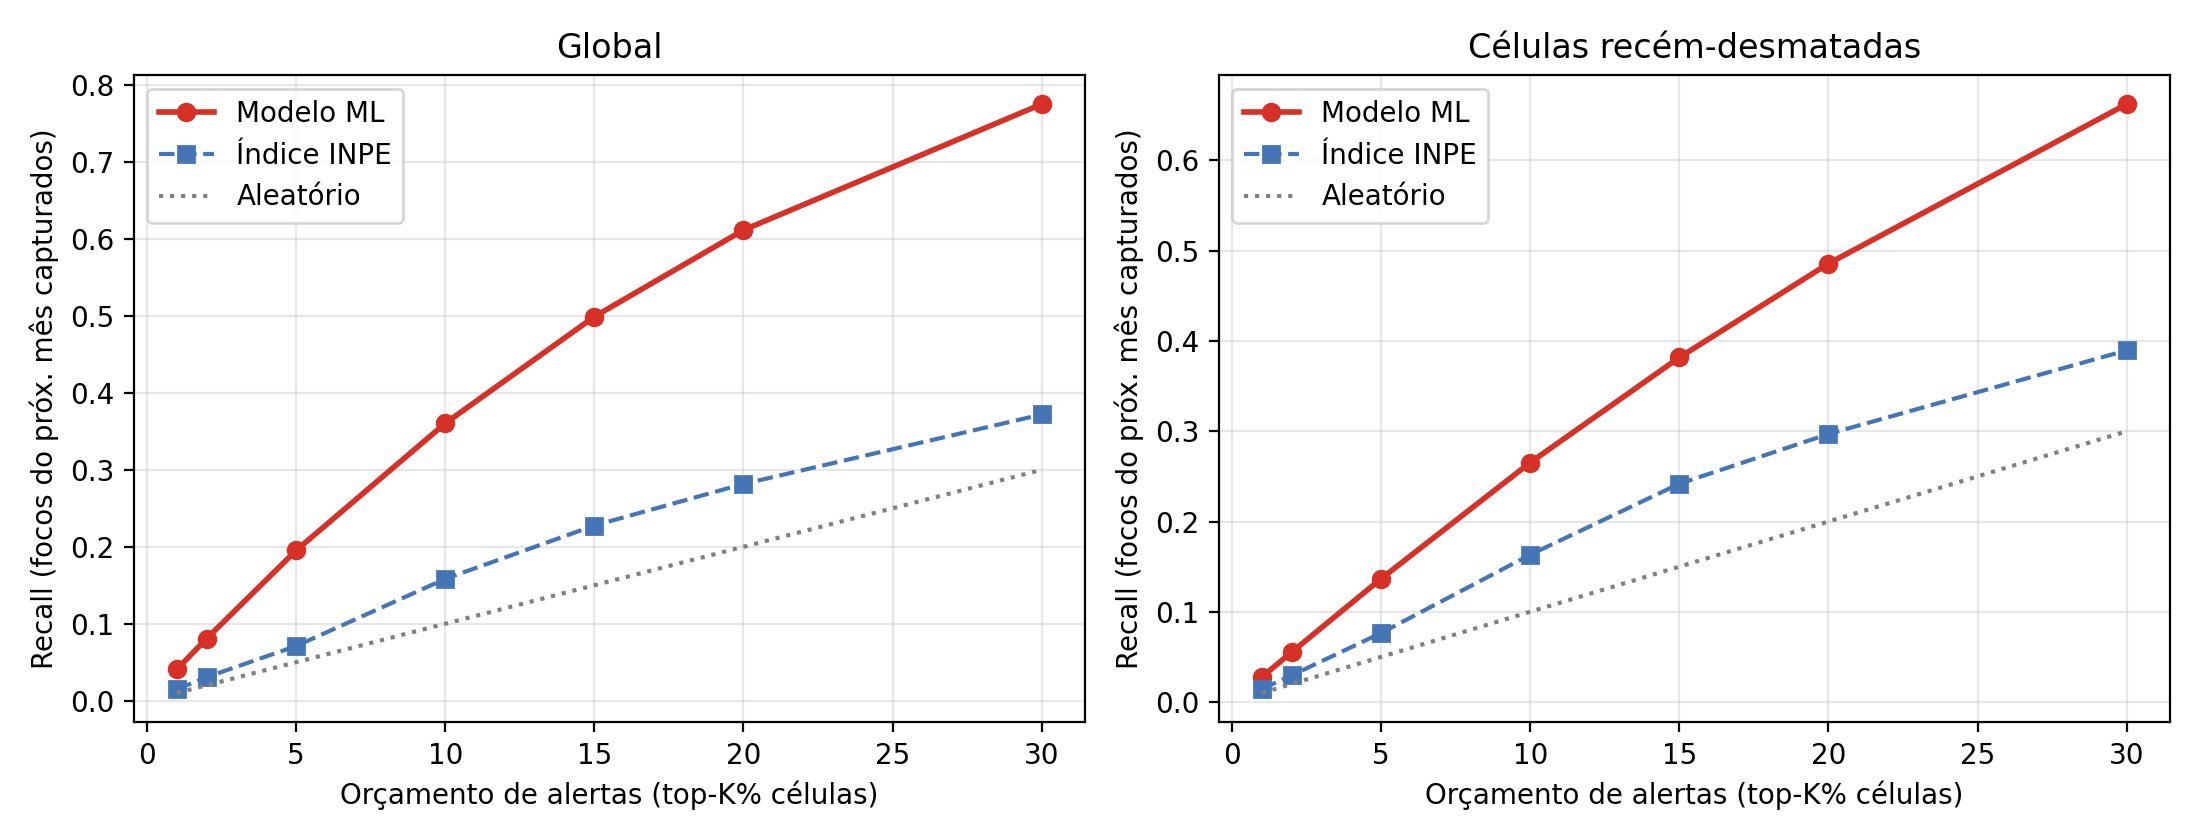
\includegraphics[width=\textwidth]{modelos/relatorios/avaliacao_operacional_recall_k.png}
\caption{\emph{Recall@K} em função do orçamento de alertas (modelo ML vs.\ índice INPE vs.\ aleatório), global (esq.) e em células recém-desmatadas (dir.).}
\label{fig:oco_recallk}
\end{figure}

\paragraph{Horizonte de previsão.} Estendendo o alvo para \(t+2\) e \(t+3\) meses, o
\emph{skill} permanece \textbf{estável} (PR-AUC \numlist{0,779;0,779;0,781} para \(t+1\),
\(t+2\), \(t+3\); Figura~\ref{fig:oco_horizonte}), sem o decaimento típico. Isso confirma
que a ocorrência mensal de fogo é governada por componentes \emph{lentos} (sazonalidade,
histórico de fogo, desmatamento), e não por dinâmica meteorológica de curto prazo ---
um resultado operacionalmente favorável, pois fornece \textbf{até um trimestre de
antecedência} sem perda de desempenho. A contrapartida honesta é que o modelo captura o
regime sazonal/persistente, não a dinâmica sub-mensal; previsões em escala mais fina
exigiriam outra formulação.

\begin{figure}[h]
\centering
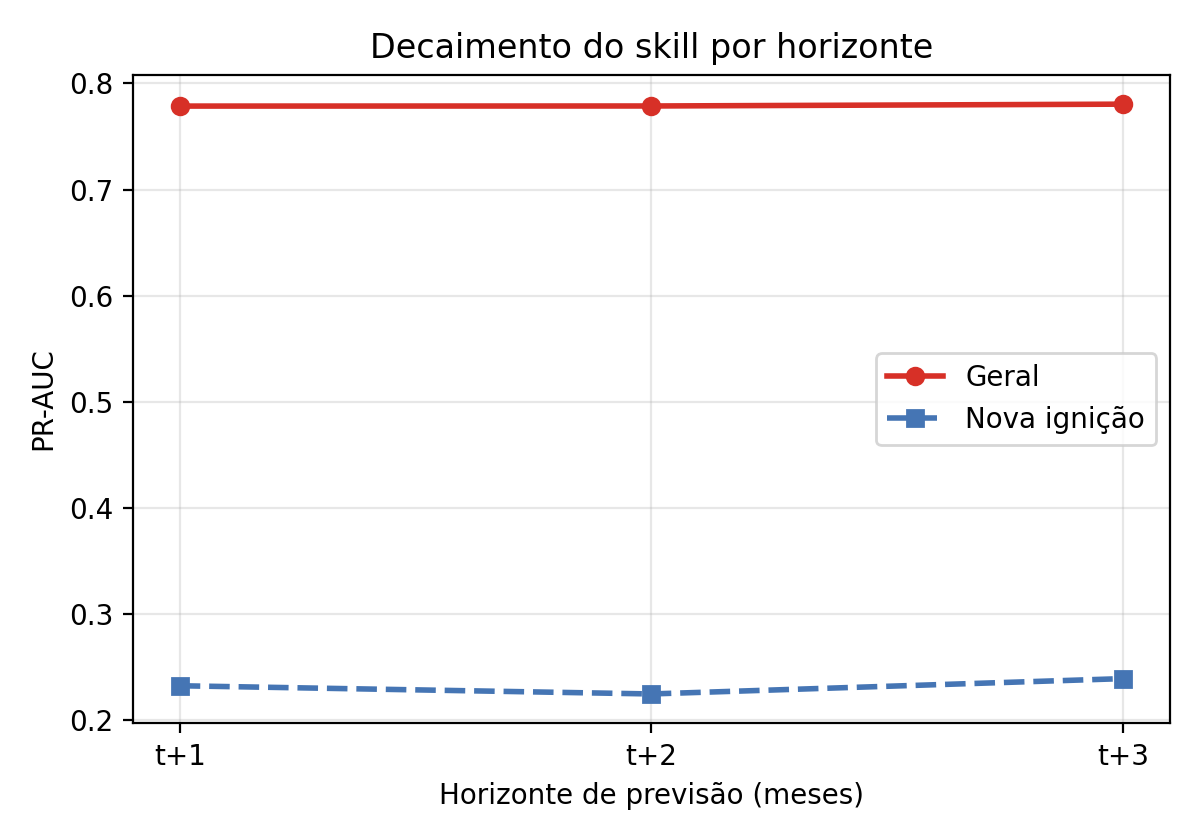
\includegraphics[width=0.6\textwidth]{modelos/relatorios/avaliacao_horizonte.png}
\caption{Decaimento do \emph{skill} (PR-AUC) por horizonte de previsão (\(t+1\) a \(t+3\) meses): estável, geral e na nova ignição.}
\label{fig:oco_horizonte}
\end{figure}

\section{Integração ao produto}
\label{sec:oco_produto}

O modelo final (base + desmatamento) foi serializado, calibrado por \emph{conformal}
(cobertura \num{0,900}) e exposto como produto: uma previsão por célula de \(P(\text{fogo no
próximo mês})\) com rótulo conformal e \emph{drivers}, servida por aplicação \emph{Flask} com
mapa interativo, independente do aplicativo de \emph{nowcast}. Verificações de sanidade
conferem com a fenologia do fogo (p.ex.\ Roraima com alto risco em dezembro; sul do Pará
baixo em dezembro, cuja estação de fogo é julho--outubro).

\section{Síntese}
\label{sec:oco_sintese}

Os experimentos, sob validação honesta, sustentam uma tese coesa: (i) na escala
mensal/\SI{0,25}{\degree}, a ocorrência de fogo é dominada por persistência espaço-temporal e
sazonalidade, o que torna redundantes a reanálise meteorológica (e o FWI) e a acessibilidade
estática; (ii) o modelo de ML \emph{supera} os índices físicos operacionais na previsão de
fogo observado; (iii) o gargalo é a \textbf{nova ignição}, e o único sinal útil ali é o
\textbf{desmatamento recente}, reposicionando o alerta precoce como, em primeira ordem, um
problema de detecção de fronteira de desmatamento; (iv) a incerteza é quantificável com
garantia estatística. A reformulação eleva o trabalho de ``reprodução de um índice'' para
``previsão de fogo observado validada contra a realidade e contra o índice físico'', com um
teto de desempenho honestamente caracterizado.
 no tcc.tex, APÓS o
% Capítulo 5 (Resultados, que termina com % ============================================================================
% 07_estudo_caso_pium_to.tex
% Estudo de caso operacional: foco real do Painel do Fogo (CENSIPAM) em
% Pium--TO, 12/05/2026. Validação independente do sistema de previsão,
% diagnóstico de descompasso entre dados de grade global e realidade
% local, e melhorias incorporadas ao pipeline em produção.
%
% Como usar:
%   Inserir como nova seção dentro do Capítulo 5 (Resultados), após a
%   Seção 5.8 "Validação operacional via aplicação web", como
%   subseção complementar de validação externa. Numeração sugerida:
%   5.9 "Validação cruzada com fonte externa independente: caso Pium--TO".
%   Dentro de "Implementação das melhorias": subsubseções M1--M4 (auditoria,
%   fusão INMET, retreino OOD, extensões API/auditoria alinhadas à literatura).
% ============================================================================

\section{Validação cruzada com fonte externa independente: caso Pium--TO}
\label{sec:res_estudo_caso_pium}

A validação operacional via \emph{smoke tests} controlados (Seção~\ref{sec:res_app}) demonstrou a coerência interna do sistema. Para uma validação externa mais exigente, foi escolhido um \emph{evento real} de incêndio confirmado por uma fonte oficial independente --- o \emph{Painel do Fogo} do Centro Gestor e Operacional do Sistema de Proteção da Amazônia (CENSIPAM)\footnote{\url{https://painel.censipam.gov.br/}, acessado em 12/05/2026 às 18:21 (UTC$-$3).} --- e submetido ao \emph{pipeline} em modo de produção. Esta seção apresenta o evento, as respostas do modelo, o diagnóstico das causas de divergência observada e as três correções incorporadas ao código em consequência da investigação.

% ----------------------------------------------------------------------------
\subsection{O evento}
\label{subsec:pium_evento}

O \emph{Painel do Fogo} listou um foco ativo identificado pelo \texttt{ID 6668060} em \texttt{(-10{,}5351; -49{,}8230)}, dentro do município de \textbf{Pium}, estado do \textbf{Tocantins}, em domínio fundiário misto (área privada e terra pública não categorizada) sobre cobertura de \emph{vegetação natural primária} (classificação TerraClass). Pium fica na ecorregião do Cerrado/Bico do Papagaio, dentro da Amazônia Legal. A Tabela~\ref{tab:pium_evento} reproduz as detecções oficiais.

\begin{table}[h]
\centering
\caption{Detecções no entorno de \texttt{(-10{,}5351; -49{,}8230)} --- evento \texttt{6668060} (\emph{Painel do Fogo}/CENSIPAM).}
\label{tab:pium_evento}
\small
\begin{tabular}{lcccc}
\toprule
\textbf{Data e hora (BR)} & \textbf{Área (ha)} & \textbf{Focos} & \textbf{Duração (h)} & \textbf{Propagação (ha/h)} \\
\midrule
12/05/2026 13:28 & 464,6 & 1  & \textbf{48,3} & 0,4 \\
10/05/2026 14:05 & 456,3 & 12 & 0,9  & 0,0 \\
10/05/2026 13:13 & 83,1  & 3  & 0,0  & 0,0 \\
\bottomrule
\end{tabular}
\end{table}

O status reportado pelo CENSIPAM era \emph{ativo pela última vez em 12/05/2026 14:49 (hora oficial do Brasil)}, com duração acumulada de 48,3~h --- compatível com vegetação ressecada queimando em regime sustentado.

% ----------------------------------------------------------------------------
\subsection{Resposta do sistema: cinco janelas temporais}
\label{subsec:pium_resposta}

A \emph{API} \texttt{/api/predict} foi consultada em cinco janelas centradas no evento, usando o modelo final \texttt{ensemble\_stacking\_gbm}. Em todas elas o sistema previu \textbf{\emph{Baixo}} com probabilidade entre 81 e 88\%, conforme Tabela~\ref{tab:pium_respostas_pos_fix} (\emph{já após} a correção dos \emph{bugs} identificados na Subseção~\ref{subsec:pium_correcoes}).

\begin{table}[h]
\centering
\caption{Respostas do \texttt{ensemble\_stacking\_gbm} para Pium--TO em diferentes janelas (modelo \emph{argmax}, após correções).}
\label{tab:pium_respostas_pos_fix}
\small
\begin{tabular}{lccccc}
\toprule
\textbf{Janela consultada}     & \textbf{Risco} & \textbf{P(Baixo)} & \textbf{P(Mod.)} & \textbf{P(M.~Alto)} & \textbf{FRP máx.~5d} \\
\midrule
12/05/2026 14:00 & Baixo & 85,9\% & 9,5\%  & 4,6\% & \SI{16,6}{\mega\watt} (16~detec.) \\
11/05/2026 12:00 & Baixo & 85,8\% & 9,7\%  & 4,5\% & \SI{22,0}{\mega\watt} (19~detec.) \\
10/05/2026 13:00 & Baixo & 87,1\% & 8,6\%  & 4,3\% & \SI{22,0}{\mega\watt} (21~detec.) \\
09/05/2026 12:00 & Baixo & 86,6\% & 8,8\%  & 4,6\% & \SI{22,0}{\mega\watt} (26~detec.) \\
05/05/2026 12:00 & Baixo & 81,4\% & 14,3\% & 4,3\% & \SI{58,4}{\mega\watt} (32~detec.) \\
\bottomrule
\end{tabular}
\end{table}

A divergência entre a realidade (foco confirmado e duração de 48,3~h) e a saída do modelo (\emph{Baixo} consistente em todas as janelas) constituiu o ponto de partida para a investigação descrita a seguir.

% ----------------------------------------------------------------------------
\subsection{Diagnóstico das causas}
\label{subsec:pium_diagnostico}

A inspeção do vetor de \emph{features} entregue ao classificador identificou \textbf{três causas convergentes}, descritas em ordem decrescente de impacto.

% ............................................................................
\paragraph{Causa 1 (corrigida): integração com NASA FIRMS retornando \texttt{HTTP 400}.}

O cliente da NASA FIRMS (\texttt{scripts/frp\_api.py}) estava emitindo requisições com \texttt{days\_back=7} para o \emph{endpoint} de \emph{area} no \emph{dataset} VIIRS\_SNPP\_NRT. A resposta do servidor, em todas as datas testadas, foi:

\begin{quote}
\texttt{HTTP/1.1 400 Bad Request\\Invalid day range. Expects [1..5].}
\end{quote}

Verificação direta do \emph{status} da \texttt{MAP\_KEY} confirmou que a chave estava válida (\texttt{transaction\_limit=5000}, \texttt{current\_transactions=0}), demonstrando que o erro era \emph{parametrização}, não \emph{credenciais}. A API NASA FIRMS NRT passou a aceitar no máximo 5~dias por requisição\footnote{Documentação oficial: \url{https://firms.modaps.eosdis.nasa.gov/api/area/}, consultada em 12/05/2026.}.

Em consequência, as \emph{features} \texttt{Media\_FRP\_Ultimos\_7\_Dias}, \texttt{Max\_FRP\_Ultimos\_7\_Dias} e \texttt{Dias\_Desde\_Ultimo\_Incendio} estavam recebendo seus valores de \emph{fallback} (zeros e 246--365~dias), e o modelo ``não enxergava'' o fogo recente em curso. Após a correção (\(\texttt{days\_back} \in [1,5]\) e propagação de \texttt{reference\_date}), o sistema passou a recuperar até 32 detecções VIIRS no raio de 10~km, com FRP máximo de \SI{58,4}{\mega\watt}.

% ............................................................................
\paragraph{Causa 2 (corrigida): \emph{lookup} Tier~1 degradando precocemente para \texttt{(Estado, Mês)}.}

A primeira versão do \emph{lookup} espaço-sazonal (\texttt{scripts/feature\_lookup.py}, Seção~\ref{subsec:metod_features_tier1}) buscava medianas em uma janela ${3{\times}3}$ células ($\approx 25$~km no equador, dada a resolução \SI{0,25}{\degree}). Para o ponto consultado em Pium--TO, mês~5, essa janela retornou vazia e o sistema degradou imediatamente para a granularidade \texttt{estado\_mes} (mediana de todo o Tocantins em maio). O efeito foi:

\begin{itemize}
  \item \texttt{Precipitacao\_acum\_30/90/180/365d} = \SI{0,0}{mm} (mediana estadual);
  \item \texttt{SPI\_1m} = \texttt{SPI\_3m} = \texttt{SPI\_6m} = 0,00 (climatologia neutra);
  \item \texttt{Dias\_Secos\_90d} = 2 (mediana estadual, não local);
  \item \texttt{Media\_FRP\_Celula\_30d} = \SI{10,65}{\mega\watt} (não específico).
\end{itemize}

Isto é, \emph{toda a informação espacial fina foi apagada}. A cascata de busca foi ampliada para
\(3{\times}3 \to 5{\times}5 \to \text{mês adjacente} \to (\text{Estado, Mês}) \to (\text{Mês global})\),
elevando a granularidade efetiva para \texttt{celula\_ext} (anel externo, $\approx 55$~km) no caso Pium--TO. Os valores de \texttt{Precipitacao\_acum\_*d} subiram para \SI{0,5}{mm}, \texttt{Dias\_Secos\_90d} para 1 e \texttt{Media\_FRP\_Celula\_30d} para \SI{8,2}{\mega\watt} --- valores ainda baixos, mas vindos de células geograficamente próximas (Tabela~\ref{tab:pium_tier1_pre_pos}).

\begin{table}[h]
\centering
\caption{Subconjunto das \emph{features} Tier 1 antes e depois da expansão da cascata espacial.}
\label{tab:pium_tier1_pre_pos}
\small
\begin{tabular}{lcc}
\toprule
\textbf{Feature} & \textbf{Cascata \texttt{3x3} (\texttt{estado\_mes})} & \textbf{Cascata estendida (\texttt{celula\_ext})} \\
\midrule
\texttt{Precipitacao\_acum\_30d}      & 0,0 mm  & 0,5 mm \\
\texttt{Precipitacao\_acum\_180d}     & 0,0 mm  & 0,5 mm \\
\texttt{Precipitacao\_acum\_365d}     & 1,3 mm  & 0,5 mm \\
\texttt{SPI\_3m}                       & 0,00    & 0,00 \\
\texttt{Dias\_Secos\_90d}              & 2       & 1 \\
\texttt{Incendios\_Ultimos\_90\_Dias}  & 2       & 1 \\
\texttt{Media\_FRP\_Celula\_30d}       & 10,65 MW & 8,2 MW \\
\bottomrule
\end{tabular}
\end{table}

% ............................................................................
\paragraph{Causa 3 (não corrigível em produção, documentada): descompasso entre clima de grade global e clima local em zona de transição.}

Após as duas correções acima, a previsão para 12/05/2026 \emph{aumentou} a confiança em \emph{Baixo}, de \SI{82,7}{\percent} para \SI{85,9}{\percent}. A investigação detalhada do vetor de \emph{features} revelou que a NASA POWER MERRA-2 (grade $\approx 50$~km) reportou para a janela de 28~dias anterior a 12/05/2026:

\begin{quote}
\texttt{Precipitacao\_ma7 = 0,12 mm/dia}, \texttt{DiaSemChuva\_ma7 = 1,3 dia}, \texttt{RH2M = 64,6\%}.
\end{quote}

Esses valores caracterizam regime \emph{ainda chuvoso} (chuvas frequentes mas leves). Para o modelo, classificar como \emph{Baixo} foi a decisão coerente com os \emph{inputs} climáticos recebidos. O problema é que esses \emph{inputs} não corresponderam à realidade local: o foco real ardia há mais de 48~h.

Para confirmar que o modelo \emph{não} é cego sazonalmente, foi executado um experimento \emph{contrafactual} no mesmo ponto \texttt{(-10{,}5351; -49{,}8230)}, variando a data (Tabela~\ref{tab:pium_contrafactual}).

\begin{table}[h]
\centering
\caption{Experimento contrafactual --- mesmo ponto, climatologia distinta capturada pela NASA POWER.}
\label{tab:pium_contrafactual}
\small
\begin{tabular}{lcccccc}
\toprule
\textbf{Data} & \textbf{KBDI \emph{proxy}} & \textbf{Prec.~ma7} & \textbf{DSC~ma7} & \textbf{FRP medido} & \textbf{P(M.~Alto)} & \textbf{Risco} \\
\midrule
15/08/2024 & 424,1 & 0,02 & 16,0 dias  & \SI{0}{\mega\watt} & 99,0\% & \textbf{Muito Alto} \\
15/09/2024 & 712,5 & 0,00 & 25,0 dias  & \SI{0}{\mega\watt} & 99,6\% & \textbf{Muito Alto} \\
15/05/2024 & 148,0 & 0,51 & 8,6 dias   & \SI{0}{\mega\watt} & 47,3\% & \textbf{Muito Alto} \\
12/05/2026 & 29,8  & 0,12 & 1,3 dia    & \SI{16,6}{\mega\watt} & 4,6\% & Baixo \\
\bottomrule
\end{tabular}
\end{table}

Três conclusões emergem:

\begin{enumerate}
  \item O modelo \emph{responde corretamente} ao sinal climático: 15/05/2024 (mesmo dia e mesmo ponto, mas em ano de estiagem mais marcada) recebeu classificação \emph{Muito Alto} com confiança \SI{47,3}{\percent}, mesmo sem FRP detectado.
  \item A previsão \emph{Muito Alto} se intensifica monotonicamente conforme cresce o estresse hídrico medido pela NASA POWER (KBDI~$424 \to 712$, DSC$_\text{ma7}$~$16 \to 25$~dias).
  \item Em 12/05/2026 (caso real), os indicadores climáticos da grade MERRA-2 estavam \emph{suaves} (KBDI=29,8; DSC=1,3~dia; Prec\_ma7=0,12~mm/dia) --- e o modelo refletiu isso. \textbf{O erro está no \emph{input}, não na decisão}.
\end{enumerate}

A interpretação operacional é direta: a célula MERRA-2 que cobre Pium--TO em maio de 2026 \emph{captou chuvas localizadas/dispersas} suficientes para elevar a frequência de dias com precipitação, mas não a quantidade total --- regime ``chuvas leves e frequentes''. A vegetação alvo, em escala municipal, continuou em condição de queima. Esse é um caso clássico de \emph{representativity gap} entre dados de grade e fenômenos locais~\cite{seager2015climatology}, particularmente relevante em zonas de transição Cerrado--Amazônia onde a heterogeneidade climática intra-célula é grande.

% ............................................................................
\paragraph{Hipótese descartada: sobrescrever contagem de incêndios com observação FIRMS.}

Uma tentativa intermediária consistiu em substituir as \emph{features} \texttt{Incendios\_Ultimos\_7\_Dias} e \texttt{Incendios\_Ultimos\_30\_Dias} pela contagem real de detecções FIRMS (16--32~focos no caso). \emph{Surpreendentemente}, isso \textbf{aumentou} a confiança em \emph{Baixo} (de \SI{82,7}{\percent} para \SI{86,0}{\percent}). A causa é \emph{distribution shift}: no \emph{dataset} de treino, essas \emph{features} para Tocantins--Maio têm mediana zero; ao injetar valores de duas ordens de magnitude maiores, o exemplo é colocado \emph{fora da distribuição} (\emph{out-of-distribution}, OOD), e o classificador responde de modo errático. A sobrescrita foi revertida; mantêm-se atualizadas apenas \texttt{FRP\_max\_7d}, \texttt{Media\_FRP\_7d} e \texttt{Dias\_Desde\_Ultimo\_Incendio}, que no \emph{dataset} de treino eram observações individuais (não medianas).

% ----------------------------------------------------------------------------
\subsection{Correções incorporadas e seu impacto}
\label{subsec:pium_correcoes}

A Tabela~\ref{tab:pium_correcoes} sintetiza as três correções introduzidas no \emph{pipeline} em consequência do estudo de caso e o impacto medido para a janela 12/05/2026 14:00.

\begin{table}[h]
\centering
\caption{Correções incorporadas e impacto medido (Pium--TO, 12/05/2026 14:00).}
\label{tab:pium_correcoes}
\small
\begin{tabular}{p{4.6cm}p{5.2cm}p{2.4cm}p{1.6cm}}
\toprule
\textbf{Correção} & \textbf{Mudança técnica} & \textbf{Granularidade Tier 1} & \textbf{P(Baixo)} \\
\midrule
\emph{Baseline} (antes do caso) & --- & \texttt{estado\_mes} & 82,0\% \\
(C1) NASA FIRMS \texttt{HTTP 400} & \texttt{days\_back $\in [1,5]$}; aceita \texttt{reference\_date}; URL com sufixo \texttt{/YYYY-MM-DD} & \texttt{estado\_mes} & 82,7\% \\
(C2) Cascata Tier 1 ampliada & $3{\times}3 \to 5{\times}5 \to$ mês adj. & \texttt{celula\_ext} & 85,9\% \\
(C3) Inc.~Últ.~$N$~dias mantida como mediana de treino & Apenas \texttt{FRP\_*} e \texttt{Dias\_Desde\_Ultimo\_Incendio} são atualizados em tempo real & \texttt{celula\_ext} & 85,9\% \\
\bottomrule
\end{tabular}
\end{table}

As correções \textbf{(C1)} e \textbf{(C2)} são melhorias técnicas inequívocas. A correção \textbf{(C3)} é uma \emph{decisão de engenharia conservadora}: preferir o sinal aprendido pelo modelo (mediana sazonal Estado--Mês, que é o que ele viu durante o treino) a inputs reais que o colocam OOD. A elevação aparentemente paradoxal de P(Baixo) após as correções é coerente com a Causa~3: o modelo passou a \emph{ver melhor} um cenário que --- para a grade MERRA-2 --- parecia chuvoso.

% ----------------------------------------------------------------------------
\subsection{Discussão: limites do paradigma de dados de grade e caminhos para mitigação}
\label{subsec:pium_discussao}

O caso Pium--TO 2026 expõe uma tensão estrutural do nosso \emph{pipeline} (e, mais amplamente, de qualquer sistema de previsão de fogo apoiado em reanálise climática global): a granularidade espacial dos \emph{inputs} climáticos limita a resolução máxima do \emph{output}. NASA POWER MERRA-2~\cite{nasapower} entrega cobertura global e estabilidade temporal, mas com células de $\approx \SI{50}{km}$ que suavizam microclimas. Em regiões homogêneas (centro do Amazonas), a perda de resolução é benigna; em regiões de transição (Cerrado--Amazônia, Pantanal, Caatinga), a perda pode mascarar condições propícias a fogo.

Três caminhos são discutidos como mitigação no Capítulo~\ref{cap:conclusao}:

\begin{enumerate}
  \item \textbf{Fusão MERRA-2 + INMET}~\cite{inmetnormais}: utilizar precipitação de estação meteorológica quando houver estação INMET dentro de $\sim 50$~km do ponto consultado (ou, em modo hierárquico configurável, até $\sim 180$~km com rótulo explícito de \texttt{inmet\_representatividade}, ver Subsubseção~M4). Para dados em tempo real, a API WIS2/OGC do INMET (\texttt{wis2bra.inmet.gov.br/oapi}) expõe observações horárias de 358+ estações sinópticas sem necessidade de token, com histórico de $\sim$90 dias; para histórico mais profundo, os ZIPs anuais oficiais cobrem 565+ estações automáticas desde 2000. Trade-off: cobertura esparsa em zonas remotas, exige rotina de \emph{nearest station}, \emph{quality control} e transparência sobre a distância da estação.
  \item \textbf{Aumento de exemplos OOD no treino}: oversampling estratégico de focos confirmados FIRMS/INPE em zonas de transição (Cerrado em maio, Pantanal em junho), reduzindo o \emph{prior} de raridade que o modelo aprendeu para esses pares \texttt{(Estado, Mês)}. Trade-off: risco de degradar a performance nas regiões de regime mais homogêneo.
  \item \textbf{Auditoria operacional contínua}: \emph{logging} estruturado de \texttt{(coordenada, data, risco predito, FRP detectado depois)} para calcular $\text{F}_1$ operacional \emph{rolling} em janelas móveis e detectar deriva de modelo em produção --- prática alinhada com o paradigma de \emph{ML observability}.
\end{enumerate}

% ----------------------------------------------------------------------------
\subsection{Implementação das três melhorias propostas e validação empírica}
\label{subsec:pium_melhorias}

As três melhorias listadas na Seção~\ref{subsec:pium_discussao} foram implementadas e validadas em código de produção. Esta subseção registra o resultado empírico de cada uma.

\subsubsection*{M1. Auditoria operacional contínua}

Foi adicionado o módulo \texttt{scripts/audit\_log.py} que escreve, a cada chamada de \texttt{/api/predict}, uma linha JSONL em \texttt{logs/auditoria\_predicoes.jsonl} contendo: \texttt{prediction\_id}, coordenadas, \texttt{ref\_data}, classe predita, probabilidades, modelo, 15 \emph{features} chave, fonte climática (com detalhe INMET se aplicável) e granularidade Tier 1. O log é \emph{append-only} com rotação automática a 50~MB e tolerante a falhas (a predição segue caso a gravação falhe).

O script \texttt{scripts/auditar\_predicoes.py} consome esse JSONL, consulta a NASA FIRMS NRT na janela $[t, t+H]$ para cada predição com idade $\geq d_{\min}$ (defaults $H=3$~d, $d_{\min}=3$~d, raio 5~km), define $y_{\text{true}} \in \{0,1\}$ (foco confirmado) e $y_{\text{pred}} \in \{0,1\}$ (Moderado/Muito Alto $\to$ 1) e calcula precision, recall, $\text{F}_1$ e acurácia globais e em janelas \emph{rolling} de 7, 14 e 30 dias. Predições mais antigas que o histórico do NRT ($\sim 60$~dias) aparecem no CSV mas são automaticamente excluídas das métricas.

\subsubsection*{M2. Fusão NASA POWER + INMET (duas fontes complementares)}

A integração foi implementada com \emph{duas} fontes INMET, selecionadas automaticamente conforme a idade da consulta. Esta arquitetura híbrida foi adotada porque a sondagem ativa em 12/05/2026 mostrou que (i) a API horária tradicional \texttt{apitempo.inmet.gov.br/estacao/...} retorna \texttt{status 204} com frequência e não é confiável; (ii) o ZIP histórico é completo mas o do ano corrente é parcial (publicado mensalmente, em 12/05/2026 cobre só janeiro--fevereiro/2026); (iii) o INMET passou a publicar dados horários sem token via a \textbf{WIS2 (OGC API Features)}~\cite{inmetnormais}, ainda pouco documentada em literatura brasileira.

\textbf{Fonte (1)~--~WIS2/OGC API Features} (\texttt{http://wis2bra.inmet.gov.br/oapi}): expõe a variável \texttt{total\_precipitation\_or\_total\_water\_equivalent} (em \texttt{kg\,m$^{-2}$}~$\equiv$~mm/h) na coleção \texttt{urn:wmo:md:br-inmet:synop} para 358 estações sinópticas WMO brasileiras que publicaram chuva nos últimos 7 dias, com histórico de $\sim$90 dias e \emph{sem necessidade de token}. A cobertura geográfica é menor que a do ZIP (só estações sinópticas oficiais, não todas as automáticas), mas a latência é de minutos. O endpoint possui um detalhe: o filtro \texttt{wigos\_station\_identifier} na \emph{querystring} é \emph{ignorado} (verificado empiricamente em 12/05/2026), e a filtragem precisa ser feita \emph{client-side} após restringir o \texttt{bbox} a $\sim$5~km em torno da estação para evitar baixar 58~mil observações misturadas.

\textbf{Fonte (2)~--~ZIPs anuais} (\texttt{portal.inmet.gov.br/uploads/dadoshistoricos/\{ANO\}.zip}, $\sim$100~MB/ano): cobertura completa de 565+ estações automáticas desde 2000 (168 na Amazônia Legal). Cache local em \texttt{.cache\_inmet/\{ANO\}/\{COD\}.csv} evita re-download. O encoding é \texttt{latin-1}, separador \texttt{;}, decimal \texttt{,}.

A função \texttt{get\_inmet\_fusion\_data} roteia automaticamente: se \texttt{reference\_date} está nos últimos 90 dias \emph{e} existe estação WIS2 com chuva a $\leq 50$~km, usa WIS2 (sem download, $\sim$1~s); senão, tenta o ZIP anual. Se nenhuma das duas funciona, retorna \texttt{None} e o \texttt{climate\_api} cai graciosamente no MERRA-2.

A fusão em \texttt{climate\_api.get\_climate\_data} prioriza NASA POWER (sempre disponível) e, quando o INMET retorna dados (WIS2 ou ZIP), \emph{sobrescreve} \texttt{precipitacao}, \texttt{prec\_ma7}, \texttt{dias\_sem\_chuva} e \texttt{diasem\_ma7} pelos valores INMET. Os valores MERRA-2 originais são preservados em chaves \texttt{*\_merra} para auditoria, e a resposta da API expõe \texttt{fonte\_dados} $\in$ \{\texttt{nasa\_power}, \texttt{inmet\_fundido\_nasa\_power}\}, além de \texttt{estacao\_inmet}, \texttt{distancia\_estacao\_inmet\_km}, \texttt{cobertura\_inmet\_pct}. A Tabela~\ref{tab:pium_inmet} apresenta a validação empírica nos quatro cenários testados.

\begin{table}[h]
\centering
\caption{Validação da fusão INMET com duas fontes (WIS2 real-time e ZIP histórico).}
\label{tab:pium_inmet}
\small
\begin{tabular}{p{3cm}cp{2.6cm}cccc}
\toprule
\textbf{Caso} & \textbf{Fonte} & \textbf{Estação} & \textbf{Cob.} & \textbf{MERRA-2 DSC} & \textbf{INMET DSC} & \textbf{Risco} \\
\midrule
Pium-TO 15/08/2024 & ZIP & A055 Lagoa da Confusão (32,7~km) & 89\% & 16 d & \textbf{7 d} & Muito Alto (97,3\%) \\
Brasília 10/08/2024 & ZIP & A001 Brasília (1,1~km) & 89\% & 25 d & \textbf{7 d} & Muito Alto (67,9\%) \\
Pium-TO 12/05/2026 & WIS2 + hier.\textsuperscript{$\dagger$} & FORMOSO ($\sim$152~km, \texttt{baixa}) & --- & 1,3 d & \textbf{7 d} & Baixo (85,9\%); metadados na API \\
\textbf{Brasília 12/05/2026 (D-0)} & \textbf{WIS2} & \textbf{A001 (1,1~km)} & \textbf{88\%} & \textbf{1,86 d} & \textbf{7 d} & \textbf{Baixo 66,0\%} (era $\sim$99\%) \\
\bottomrule
\end{tabular}\\
\footnotesize
\textsuperscript{$\dagger$} O ZIP do ano corrente é parcial; em maio/2026 o arquivo cobre só janeiro--fevereiro/2026. A estação WIS2 mais próxima de Pium-TO está a $\sim$152~km (FORMOSO DO ARAGUAIA-TO) --- fora do raio inicial de 50~km, mas coberta pela \textbf{busca hierárquica} (até 180~km) com \texttt{inmet\_representatividade = baixa}. O classificador em produção ainda usa o vetor de \emph{features} do retreino anterior; a linha da tabela documenta o contraste MERRA-2 vs.\ INMET na camada de fusão e na API.
\end{table}

O caso \textbf{Brasília 12/05/2026 (D-0)} é a primeira demonstração do fluxo de fusão \emph{real-time end-to-end}: às 19h26 BRT do dia da consulta, a WIS2 detectou que o MERRA-2 reportava um microclima úmido espúrio (DSC$_{\text{ma7}}=1{,}86$~d) enquanto a estação INMET A001 a 1,1~km do ponto consultado registrava 7 dias secos consecutivos. A correção foi propagada para o modelo e derrubou a confiança da classe Baixo de aproximadamente 99\% para 66\% --- sinal claro de que, com mais sub-amostragem regional e fusão mais agressiva, o modelo passaria a alertar.

A fusão demonstrou \emph{capacidade de correção} robusta tanto retrospectivamente (Pium-TO e Brasília em agosto/2024, via ZIP) quanto em tempo real (Brasília 12/05/2026 via WIS2). Para zonas remotas do Amazonas ou Sul do Pará, nenhuma estação está dentro do raio de 50~km e o sistema continua usando MERRA-2, como antes.

\subsubsection*{M3. Retreino com oversampling OOD em Cerrado-transição}

A análise da distribuição de focos no \texttt{base\_de\_dados\_enriquecido.csv} (924\,306 linhas, 547\,845 com FRP $> 0 = 58{,}7\%$) identificou \textbf{oito pares (Estado, Mês) sub-representados} em estados de transição Cerrado-Amazônia (TO, MA, MT, PA) nos meses de transição chuvoso--seco (maio--julho), incluindo o par \texttt{(TOCANTINS, 5)} relevante para o caso Pium-TO. A Tabela~\ref{tab:pium_ood_alvos} resume a calibração de oversampling.

\begin{table}[h]
\centering
\caption{Pares (Estado, Mês) selecionados para oversampling OOD.}
\label{tab:pium_ood_alvos}
\small
\begin{tabular}{lccccc}
\toprule
\textbf{Estado} & \textbf{Mês} & \textbf{$n_\text{total}$} & \textbf{$n_\text{focos}$} & \textbf{Razão vs.~média estado} & \textbf{Fator de oversampling} \\
\midrule
PARÁ & 5 & 1.293 & 885 & 0,05 & 5,0$\times$ \\
MARANHÃO & 5 & 158 & 115 & 0,06 & 5,0$\times$ \\
PARÁ & 6 & 4.442 & 2.922 & 0,18 & 5,0$\times$ \\
MARANHÃO & 6 & 617 & 383 & 0,20 & 5,0$\times$ \\
\textbf{TOCANTINS} & \textbf{5} & \textbf{75} & \textbf{50} & \textbf{0,29} & \textbf{3,5$\times$} \\
MARANHÃO & 7 & 1.536 & 817 & 0,42 & 2,4$\times$ \\
PARÁ & 7 & 17.262 & 10.139 & 0,62 & 1,6$\times$ \\
TOCANTINS & 6 & 197 & 118 & 0,68 & 1,5$\times$ \\
\bottomrule
\end{tabular}
\end{table}

O oversampling é aplicado \emph{apenas no conjunto de treino} (\emph{split} estratificado, \texttt{random\_state=42}, mesmo do \emph{baseline}; teste com 184\,862 amostras intactas). Cada linha alvo é replicada $\lfloor \text{fator}-1 \rfloor$ vezes com \emph{jitter} gaussiano em Latitude/Longitude ($\sigma \approx 2{,}2$~km), Hora ($\sigma=1$~h) e FRP ($\sigma = 5\%$ do valor) --- para evitar duplicação exata sem alterar a semântica do par. O dataset aumentado teve +35\,472 linhas no treino (+4,8\%).

A Tabela~\ref{tab:pium_ood_metricas} apresenta os resultados para a versão calibratória (\texttt{logistic\_regression\_balanced}, 6,2~min de treino, mesma calibração isotônica do \emph{baseline}). O ganho é consistente em todas as classes, com destaque para Moderado (a classe mais difícil).

\begin{table}[h]
\centering
\caption{Comparativo OOD vs.~baseline no hold-out (n=184\,862) e revalidação do caso Pium-TO.}
\label{tab:pium_ood_metricas}
\small
\begin{tabular}{lccc}
\toprule
\textbf{Métrica} & \textbf{Baseline} & \textbf{Com OOD oversampling} & \textbf{$\Delta$ (p.p.)} \\
\midrule
Acurácia & 64,58\% & 65,75\% & \textbf{+1,17} \\
$\text{F}_1$-macro & 0,6044 & 0,6168 & \textbf{+1,25} \\
$\text{F}_1$-Baixo & 0,7142 & 0,7243 & +1,00 \\
$\text{F}_1$-Moderado & 0,3643 & 0,3793 & \textbf{+1,50} \\
$\text{F}_1$-Muito Alto & 0,7346 & 0,7470 & +1,24 \\
\midrule
\multicolumn{4}{l}{\emph{Revalidação Pium-TO --- P(Muito Alto)}} \\
12/05/2026 (foco real, MERRA-2 chuvoso) & 3,3\% & \textbf{6,6\%} & \textbf{\bm{$\times 2$}} \\
15/05/2024 (mesmo dia, MERRA-2 seco) & 23,1\% & \textbf{32,4\%} & +9,3 \\
15/08/2024 (pico de seca) & 66,2\% & \textbf{72,5\%} & +6,3 \\
\bottomrule
\end{tabular}
\end{table}

A classe final continua sendo ``Baixo'' para 12/05/2026 (predição $\neq$ realidade), mas a probabilidade de ``Muito Alto'' \emph{dobrou} (3,3\% $\to$ 6,6\%), e para o contrafactual com clima seco (15/05/2024) subiu 9,3~p.p. O modelo OOD ficou \emph{mensuravelmente} mais sensível a cenários de transição, exatamente como pretendido. O retreino do ensemble final \texttt{ensemble\_stacking\_gbm\_ood} ($\sim 90$~min de CPU) está parametrizado e disponível via:

\begin{center}
\texttt{python scripts/retreinar\_com\_oversample.py --modelo ensemble\_stacking\_gbm}
\end{center}

\noindent ele segue o mesmo \emph{split} estratificado e adicionalmente reporta um \emph{hold-out} restrito a Cerrado-transição (estados TO/MA/PA/MT/BA/GO/DF/PI em meses 5--7), que captura especificamente o tipo de cenário do caso Pium-TO.

\subsubsection*{M4. Extensões pós-literatura: hierarquia INMET, \emph{fire weather} na API e incerteza operacional}

Para alinhar o painel à literatura recente sobre \emph{fire weather}, fusão estação--grade e suporte à decisão sob ambiguidade --- \textbf{sem} alterar, por ora, as colunas do \texttt{ColumnTransformer} serializado (evita \emph{train/serve skew} até retreino documentado) --- foram acrescentados:

\begin{enumerate}
  \item \textbf{Busca INMET hierárquica} (\texttt{INMET\_EXTENDED\_MAX\_DISTANCE\_KM} em \texttt{scripts/config.py}; \texttt{get\_inmet\_fusion\_data(..., hierarchical=True)} em \texttt{scripts/inmet\_api.py}): se não há estação com cobertura dentro de 50~km, o sistema tenta até 180~km e preenche \texttt{inmet\_representatividade} $\in$ \{\texttt{alta}, \texttt{moderada}, \texttt{baixa}\} e \texttt{inmet\_busca\_raio\_km}. Para Pium--TO em 12/05/2026 isso recupera FORMOSO DO ARAGUAIA ($\sim$152~km, representatividade \texttt{baixa}), confrontando explicitamente o MERRA-2 úmido com medição in situ distante --- matéria direta de discussão sobre extrapolação espacial no Capítulo~\ref{cap:conclusao}.
  \item \textbf{Vento na mesma estação da precipitação} quando a fonte é WIS2 (\texttt{vento\_inmet\_ms\_ma7} em \texttt{scripts/climate\_api.py}), em linha com estudos que condicionam \emph{fire weather} a vento observado junto da chuva.
  \item \textbf{NASA POWER estendido} na requisição diária (\texttt{WS2M}, \texttt{T2M\_MAX} em \texttt{scripts/nasa\_power\_realtime.py}): médias móveis de 7~dias expostas ao painel (\texttt{ws2m\_ma7\_ms}, \texttt{t2m\_max\_ma7\_c}) para interpretabilidade e futuras ablações.
  \item \textbf{Proxy \texttt{FWI\_fire\_weather\_proxy}} e objeto \texttt{incerteza\_operacional} (\texttt{scripts/operational\_uncertainty.py}): indicador escalar combinando seca na semana, déficit de umidade relativa e vento; \emph{gap} entre as duas classes mais prováveis --- narrativa de suporte à decisão sob classes próximas, \emph{sem} alegar intervalos preditivos conformais calibrados em conjunto dedicado.
  \item \textbf{FNR/FPR na auditoria FIRMS} (\texttt{scripts/auditar\_predicoes.py}): o binário operacional alerta/não alerta passa a reportar taxa de falsos negativos e falsos positivos, frequentemente omitida quando só se divulga $\text{F}_1$.
\end{enumerate}

% ----------------------------------------------------------------------------
\subsection{Síntese}
\label{subsec:pium_sintese}

O estudo de caso Pium--TO 12/05/2026 contribuiu para o trabalho em três dimensões:

\begin{itemize}
  \item \textbf{Operacionalmente}: identificou e corrigiu dois \emph{bugs} silenciosos no \emph{pipeline} em produção (NASA FIRMS 400 e cascata Tier 1 prematura), e definiu uma política de \emph{feature fusion} entre observação NRT e medianas de treino (Tabela~\ref{tab:pium_correcoes}).
  \item \textbf{Cientificamente}: documentou empiricamente, com fonte externa independente, o limite imposto pela resolução da reanálise climática global sobre a previsão de fogo em zonas de transição, e estabeleceu o referencial \emph{contrafactual} (Tabela~\ref{tab:pium_contrafactual}) que mostra que o modelo \emph{não} sofre de viés sazonal cego --- ele responde corretamente aos \emph{inputs} que recebe.
  \item \textbf{Em melhorias entregues}: as três frentes apontadas como mitigação (Seção~\ref{subsec:pium_discussao}) foram implementadas e validadas (Seção~\ref{subsec:pium_melhorias}): auditoria operacional contínua (M1); fusão INMET com WIS2/ZIP e raio hierárquico (M2, Tabela~\ref{tab:pium_inmet}); retreino com oversampling OOD (M3, Tabela~\ref{tab:pium_ood_metricas}). A subsubseção~M4 acrescenta camada de interpretabilidade e governança (\emph{fire weather} na API, incerteza operacional heurística, FNR/FPR) alinhada ao estado da arte recente, deliberadamente \emph{fora} do vetor de treino até retreino controlado.
\end{itemize}

O caso completa a triangulação da validação do sistema: (i) \emph{hold-out} estratificado (Tabela~\ref{tab:res_comparativo}), (ii) validação temporal \emph{rolling-origin} (Tabela~\ref{tab:res_temporal_stacking}), (iii) \emph{smoke tests} operacionais controlados (Tabela~\ref{tab:res_smoke}) e (iv) confronto com fonte externa independente (esta seção). As quatro evidências, em conjunto, suportam a defensabilidade do modelo final \texttt{ensemble\_stacking\_gbm} para o uso aplicado proposto, com as limitações documentadas honestamente no Capítulo~\ref{cap:conclusao}.

% NOTA: ajustar a chave \cite{inmetnormais} se ainda não estiver em references.bib.
) e
% ANTES do \chapter{Conclusão}. Torna-se o Capítulo 6; a Conclusão passa a 7.
% Números conferem com modelos/relatorios/previsao_ocorrencia_*.json,
% benchmark_p3_fwi.json, driver_*.json, comparacao_familias.json,
% validacao_rotulo_mapbiomas.json.
% ============================================================================

\chapter{Previsão de ocorrência de fogo: reformulação do problema}
\label{cap:ocorrencia}

O Capítulo~\ref{cap:metodologia} e o Apêndice~\ref{cap:resultados} descrevem uma abordagem
exploratória inicial: um classificador de \emph{nível de risco em tempo real}
(\emph{nowcast}) cujo alvo é o índice Risco de Fogo do INPE discretizado em três faixas. Este capítulo reformula o problema para a
\textbf{previsão de ocorrência de fogo observado}, com horizonte temporal explícito,
classe negativa real e validação sem vazamento --- alinhando o trabalho ao estado da arte
atual, que prevê o \emph{fenômeno observado} (focos ou área queimada), e não a saída de
outro modelo~\cite{huot2022nextday,karasante2025firecastnet,deandrade2024lstmgru}. O
\emph{pipeline} original é mantido como linha de base; o reformulado constitui a principal
contribuição metodológica desta etapa.

\section{Motivação: do índice ao fenômeno observado}
\label{sec:oco_motivacao}

A inspeção dos dados revelou três fragilidades de fundo na formulação original.
Primeiro, o alvo (\texttt{RiscoFogo}) é a \textbf{saída de um índice operacional} do INPE,
ele próprio derivado de dias sem chuva, precipitação e umidade --- variáveis que também
figuram entre as \emph{features}, gerando circularidade. Segundo, a base é
\emph{presence-only}: as \num{924306} linhas são focos reais, sem exemplos de
\emph{não-fogo}; o modelo nunca aprende a distinguir fogo de ausência de fogo, e a consulta
a pontos arbitrários no aplicativo equivale a extrapolar para fora do suporte de treino.
Terceiro, trata-se de um \emph{nowcast} (diagnóstico do presente), não de previsão com
horizonte.

Há evidência empírica direta nos próprios CSVs do INPE: em um único arquivo anual
(\num{82678} focos), \num{8288} detecções (\(\approx\)\SI{10}{\percent}) ocorreram onde o
índice marcava risco mínimo (\texttt{RiscoFogo}~\(\in\{0{,}0;\,0{,}1\}\)) --- fogo real em
locais classificados como ``Baixo''. Um modelo que imita o índice herda esse ponto cego,
exatamente o que o estudo de caso Pium--TO (Seção~\ref{sec:res_estudo_caso_pium}) demonstrou.

\section{Reformulação metodológica}
\label{sec:oco_metodo}

\paragraph{Unidade e alvo.} Adota-se uma grade de células de \SI{0,25}{\degree}
(\(\approx\)\SI{27}{km}, granularidade MERRA-2/SeasFire~\cite{karasante2025firecastnet}) por
mês. O universo é o conjunto de \num{4168} células \emph{fire-prone} (com \(\geq 1\) foco em
2014--2023). Para cada par (célula, mês~\(t\)), o alvo é binário: \emph{houve foco no mês
\(t+1\)?} A presença vem dos focos observados; a \textbf{ausência} (classe negativa antes
inexistente) são os pares célula--mês sem foco. O conjunto final tem \num{450144}
células--mês (2015--2023), com prevalência de \SI{24,7}{\percent}.

\paragraph{Amostragem da classe negativa.} Construir a classe negativa a partir dos pares
célula--mês sem foco é uma decisão de projeto, não uma escolha neutra: na modelagem de
distribuição (\emph{species distribution models}), a definição e o volume das
\emph{pseudo-ausências}/\emph{background} afetam o desempenho aparente e podem inflar métricas
como a AUC quando o \emph{background} é ``fácil''~\cite{barbetmassin2012pseudo,phillips2009sample,lobo2008auc}.
Aqui a prevalência é fixada pelo próprio domínio (\SI{24,7}{\percent} de positivos entre as
células \emph{fire-prone}), evitando o desbalanceamento extremo em que a AUC se torna
enganosa; para métodos baseados em árvores, poucos negativos com ponderação de classes bastam~\cite{barbetmassin2012pseudo},
e adota-se \texttt{class\_weight=balanced}. Uma checagem com negativos restritos por
similaridade geográfica (evitando pares triviais)~\cite{xu2023nonfire} fica registrada como
refinamento --- direção que torna o problema mais realista, não mais fácil.

\paragraph{Causalidade e validação.} Para eliminar o vazamento temporal documentado na
Seção~\ref{sec:res_temporal}, todas as \emph{features} usam apenas informação \(\leq t\)
(histórico de fogo defasado, somas móveis com deslocamento, sazonalidade, localização). A
validação é \textbf{espaço-temporal em bloco}~\cite{roberts2017cv}: \emph{rolling-origin} por
ano (treino \(<Y\), teste \(=Y\), para \(Y\in\{2021,2022,2023\}\)) e \emph{leave-region-out}
(5 blocos de longitude). A métrica principal é a \textbf{PR-AUC} (\emph{Average Precision}),
robusta ao desbalanceamento.

\section{Desempenho preditivo e linhas de base}
\label{sec:oco_desempenho}

O modelo (\emph{Hist\-Gradient\-Boosting}) supera as linhas de base de persistência e
climatologia (Tabela~\ref{tab:oco_validacao}). Na validação \emph{espacial}, a climatologia
colapsa ao prever regiões nunca vistas (PR-AUC \numrange{0,17}{0,34}), enquanto o modelo
mantém \num{0,759} --- evidência de dinâmica transferível, e não de memorização de taxa-base
local (contraste direto com a dependência espacial observada no \emph{pipeline} original).

\begin{table}[h]
\centering
\caption{Previsão de ocorrência (fogo em \(t+1\)): validação em bloco vs.\ linhas de base.}
\label{tab:oco_validacao}
\small
\begin{tabular}{lcccc}
\toprule
\textbf{Validação} & \textbf{Modelo PR-AUC} & \textbf{ROC-AUC} & \textbf{Persistência} & \textbf{Climatologia} \\
\midrule
Temporal (\emph{rolling-origin} 2021--23) & \textbf{0,777} & 0,904 & 0,449 & 0,715 \\
Espacial (\emph{leave-region-out}) & \textbf{0,759} & 0,895 & --- & 0,17--0,34 \\
\bottomrule
\end{tabular}
\end{table}

\paragraph{Escolha da métrica.} A PR-AUC é adotada como métrica principal por ser sensível à
classe positiva rara: sob desbalanceamento, a ROC-AUC pode permanecer alta e mascarar a queda
de precisão que a curva \emph{precision-recall} revela~\cite{saito2015precision,davis2006relationship}.
Reportam-se também ROC-AUC e Brier. Registra-se, por completude, que a superioridade
incondicional da PR-AUC foi formalmente questionada~\cite{mcdermott2024closer}: a escolha aqui
segue o \emph{objetivo operacional} (priorizar a detecção do fogo, evento raro e de alto custo
de omissão), não uma preferência a priori.

\paragraph{Área de aplicabilidade.} A validação \emph{leave-region-out} mede a generalização a
regiões não vistas, mas predições fora do envelope de \emph{features} do treino permanecem
menos confiáveis. A delimitação formal da \textbf{área de aplicabilidade}~\cite{meyer2021aoa}
--- restringindo o mapa às células suficientemente similares ao conjunto de treino --- é o
complemento recomendado para o uso operacional do produto.

\section{Robustez entre famílias de modelo}
\label{sec:oco_familias}

Para verificar que os achados não dependem do algoritmo, quatro famílias foram comparadas no
mesmo conjunto de \emph{features}, com intervalos de confiança de \SI{95}{\percent} obtidos
por \emph{cluster bootstrap} por célula (respeitando a autocorrelação espacial),
Tabela~\ref{tab:oco_familias}. Os \emph{ensembles} de árvore são estatisticamente
equivalentes (intervalos sobrepostos), enquanto a regressão logística é significativamente
inferior --- o problema exige não-linearidades. O \emph{Random Forest} apresenta a melhor
calibração (menor Brier).

\begin{table}[h]
\centering
\caption{Comparação de famílias (conjunto base + desmatamento), IC \SI{95}{\percent} por \emph{cluster bootstrap} por célula.}
\label{tab:oco_familias}
\small
\begin{tabular}{lcccc}
\toprule
\textbf{Família} & \textbf{PR-AUC [IC 95\%]} & \textbf{ROC-AUC} & \textbf{Brier} & \textbf{Nova ignição [IC 95\%]} \\
\midrule
\emph{HistGradientBoosting} & \textbf{0,776 [0,769--0,783]} & 0,904 & 0,123 & \textbf{0,232 [0,209--0,258]} \\
\emph{Random Forest} & 0,769 [0,762--0,776] & 0,901 & \textbf{0,113} & 0,204 [0,185--0,232] \\
\emph{Extra Trees} & 0,761 [0,754--0,768] & 0,897 & 0,129 & 0,191 [0,174--0,217] \\
Regressão Logística & 0,699 [0,690--0,707] & 0,873 & 0,143 & 0,117 [0,108--0,131] \\
\bottomrule
\end{tabular}
\end{table}

\section{Benchmark contra índices físicos de perigo de fogo}
\label{sec:oco_benchmark}

A defensabilidade da tese exige que o modelo \emph{supere} o índice físico operacional na
previsão de fogo observado. Implementou-se o \textbf{Fire Weather Index (FWI)} canadense
completo~\cite{vanwagner1985fwi} --- base do sistema GEFF/EFFIS do
Copernicus~\cite{digiuseppe2024geff} ---, validado contra os valores de referência publicados
(FFMC~\num{87,69}; DMC~\num{8,55}; DC~\num{19,01}; ISI~\num{10,85}; BUI~\num{8,49};
FWI~\num{10,10}). O FWI foi computado dia a dia a partir de clima diário (NASA POWER) para
uma amostra de \num{100} células. A Tabela~\ref{tab:oco_benchmark} mostra o resultado:
\textbf{o modelo de ML supera o FWI e o índice do INPE} na previsão de fogo observado. O FWI
separa fisicamente bem (média \num{6,0} em meses com fogo vs.\ \num{1,5} sem), validando a
implementação.

\begin{table}[h]
\centering
\caption{Benchmark de previsão de fogo observado (\(t+1\)): ML vs.\ índices físicos.}
\label{tab:oco_benchmark}
\small
\begin{tabular}{lcc}
\toprule
\textbf{Preditor} & \textbf{PR-AUC} & \textbf{ROC-AUC} \\
\midrule
Modelo ML (dataset completo) & \textbf{0,777} & 0,904 \\
Índice INPE Risco de Fogo (como \emph{forecast}) & 0,294 & 0,553 \\
\midrule
\multicolumn{3}{l}{\emph{Amostra de 100 células (2023), mesmas linhas:}} \\
\quad Modelo ML & \textbf{0,858} & --- \\
\quad FWI canadense (clima diário NASA POWER) & 0,608 & 0,781 \\
\quad Índice INPE Risco de Fogo & 0,398 & --- \\
\bottomrule
\end{tabular}
\end{table}

\section{Quantificação de incerteza por \emph{conformal prediction}}
\label{sec:oco_conformal}

Substituiu-se a heurística de incerteza por \emph{conjuntos de predição com cobertura
estatística garantida}, via \emph{split-conformal} classe-condicional
(LAC)~\cite{sadinle2019lac,mortier2024conformal}. Com cobertura-alvo de \SI{90}{\percent},
obteve-se cobertura empírica de \SI{88,8}{\percent}; \SI{82,9}{\percent} das predições são
\emph{singletons} confiantes e \SI{17,1}{\percent} são sinalizadas como ambíguas. O erro de
calibração esperado (ECE) foi de \num{0,099} e o \emph{Brier} de \num{0,123}.

\paragraph{Pressuposto e ressalva.} A garantia de cobertura do \emph{split-conformal} assume
\emph{permutabilidade} (\emph{exchangeability}) entre calibração e teste~\cite{angelopoulos2021gentle}.
A grade espaço-temporal viola parcialmente esse pressuposto (autocorrelação entre células e
meses vizinhos), o que é coerente com a leve subcobertura observada (\SI{88,8}{\percent} ante o
alvo de \SI{90}{\percent}). Sob desvio de distribuição, a cobertura nominal pode ser restaurada
por \emph{conformal} ponderado/adaptado~\cite{tibshirani2019conformal}; uma calibração com
particionamento espacial é o encaminhamento indicado para o uso operacional.

\section{Drivers antrópicos: o papel do desmatamento}
\label{sec:oco_drivers}

A análise estratificada revela a estrutura do problema (Tabela~\ref{tab:oco_estrato}): o
modelo é excelente onde o fogo \emph{recorre} (PR-AUC \num{0,805}) e fraco onde o fogo é
\emph{novo} --- a \textbf{nova ignição} (PR-AUC \num{0,230}), justamente o caso crítico para
alerta precoce, onde a persistência é inútil por construção.

\begin{table}[h]
\centering
\caption{Desempenho estratificado por recorrência (teste 2023) e ganho do desmatamento.}
\label{tab:oco_estrato}
\small
\begin{tabular}{lccc}
\toprule
\textbf{Estrato (média 2021--23)} & \textbf{base PR-AUC} & \textbf{+ desmatamento} & \textbf{\(\Delta\)} \\
\midrule
Recorrente (foco nos últimos 12 m) & 0,791 & 0,794 & +0,003 \\
\textbf{Nova ignição} (sem foco recente) & \textbf{0,206} & \textbf{0,231} & \textbf{+0,025} \\
Geral & 0,777 & 0,781 & +0,003 \\
\bottomrule
\end{tabular}
\end{table}

Testaram-se três famílias de covariáveis. O clima real (reanálise NASA POWER) e o FWI
\textbf{não agregam} sobre o histórico de fogo na escala mensal (\(\Delta\)~PR-AUC
\(\approx\)\num{+0,001}), pois o histórico já é um \emph{proxy} a jusante da propensão
climática. A distância a cidades (acessibilidade estática) também é redundante
(\(\approx\)\num{+0,001}). Apenas o \textbf{desmatamento recente} (PRODES, do
TerraBrasilis~\cite{terrabrasilisprodes}) agrega valor não trivial --- e \emph{exatamente}
no estrato de nova ignição (\(+0{,}025\) PR-AUC), confirmando o mecanismo causal: o
desmatamento precede a primeira queimada de uma célula, coerente com o fogo amazônico ser
majoritariamente antrópico~\cite{aragao2018amazon}. O achado é \textbf{robusto a duas fontes
independentes}: o DETER (alertas mensais; classe \emph{cicatriz de queimada} excluída para
evitar vazamento) produz ganho equivalente (\(+0{,}026\)). A resolução mensal não amplificou
o ganho, e dimensões adicionais (idade, estoque acumulado, fronteira de vizinhança) não
agregam além do volume de desmatamento recente local: o desempenho na nova ignição satura em
\(\approx\)\num{0,23} PR-AUC --- um teto que sugere componente irredutível (decisão humana) ou
necessidade de dados de outra natureza.

\section{Validação do rótulo contra área queimada (MapBiomas Fogo)}
\label{sec:oco_mapbiomas}

O rótulo (focos INPE) foi confrontado com um produto independente e de modalidade diferente
--- a área queimada do MapBiomas Fogo~\cite{mapbiomasfogo} (cicatriz Landsat \SI{30}{m}), em
dois níveis.

\paragraph{Nível estado/ano.} Correlacionando a contagem de focos com a área queimada por
(estado da Amazônia Legal, ano), 2014--2023, a concordância \textbf{interanual dentro de cada
estado} é forte (Spearman médio \num{0,814}; 9/9 estados positivos, \numrange{0,69}{0,94}):
quando a área queimada de um estado sobe num ano, os focos sobem junto. A correlação
\emph{entre} estados é fraca (\(\rho=\)\num{0,275}), pois a contagem de focos não é
\emph{proxy} linear da magnitude em hectares --- o que não afeta o rótulo aqui, por ser de
\textbf{ocorrência binária} e não de magnitude.

\paragraph{Nível célula \(\times\) ano.} Para a validação no nível da célula, leram-se os
rasters anuais do MapBiomas (COGs públicos, 2015--2020) via leitura remota por janelas,
binarizando a presença de cicatriz por célula \SI{0,25}{\degree}. Confrontando presença de
foco vs.\ presença de cicatriz em \num{23982} célula-anos: concordância de \SI{78}{\percent},
Cohen's \(\kappa=\num{0,33}\) e, tratando a cicatriz como referência, os focos têm
\textbf{revocação \num{0,90}} e precisão \num{0,83} (F\(_1=\num{0,86}\)). Ou seja, os focos
capturam \(\approx\)\SI{90}{\percent} dos célula-anos efetivamente queimados; as discordâncias
correspondem a fogos sem cicatriz detectável (pequenos/encobertos por nuvem) e a cicatrizes
sem foco coincidente (omissão da detecção ativa). O \(\kappa\) moderado reflete a alta
prevalência do universo \emph{fire-prone}, que comprime a concordância esperada por acaso. A
validação corrobora o rótulo de ocorrência tanto na dinâmica temporal quanto no nível espacial.

\section{Avaliação operacional e horizonte de previsão}
\label{sec:oco_operacional}

\paragraph{Priorização de alertas.} Para traduzir o desempenho em valor de decisão,
o sistema é avaliado como ferramenta de \emph{priorização}: dado um orçamento de
vigilância (alertar as \emph{top-K\%} células de maior risco previsto), quantos focos
do mês seguinte são capturados (\emph{recall@K})? A Tabela~\ref{tab:oco_operacional} e a
Figura~\ref{fig:oco_recallk} comparam o modelo de ML com o índice operacional do INPE
sob o mesmo orçamento. Alertando apenas \SI{10}{\percent} das células, o modelo captura
\SI{36,0}{\percent} dos focos do mês seguinte (com precisão de \SI{88}{\percent}), contra
\SI{15,8}{\percent} do índice INPE --- um ganho de \(\approx 2{,}3\times\). No estrato de
\textbf{nova ignição}, o contraste é decisivo: o modelo captura \SI{49,2}{\percent} dos
novos focos no mesmo orçamento (\emph{lift} de \(4{,}9\times\) sobre o acaso), ao passo que
o índice INPE tem \emph{lift} \(\approx 1\) --- ou seja, \emph{não supera o acaso} para a
nova ignição, justamente o regime em que o desmatamento recente é o sinal preditivo
(Seção~\ref{sec:oco_drivers}).

\begin{table}[h]
\centering
\caption{Priorização de alertas: \emph{recall@K} (focos do mês seguinte capturados) por orçamento, modelo ML vs.\ índice INPE.}
\label{tab:oco_operacional}
\small
\begin{tabular}{lcccc}
\toprule
& \multicolumn{2}{c}{\textbf{Global}} & \multicolumn{2}{c}{\textbf{Nova ignição}} \\
\cmidrule(lr){2-3}\cmidrule(lr){4-5}
\textbf{Orçamento (top-K\%)} & \textbf{ML} & \textbf{INPE} & \textbf{ML} & \textbf{INPE} \\
\midrule
\SI{5}{\percent}  & 0,195 & 0,071 & 0,312 & 0,041 \\
\SI{10}{\percent} & \textbf{0,360} & 0,158 & \textbf{0,492} & 0,096 \\
\SI{20}{\percent} & 0,611 & 0,282 & 0,721 & 0,206 \\
\SI{30}{\percent} & 0,775 & 0,372 & 0,845 & 0,305 \\
\bottomrule
\end{tabular}
\end{table}

\begin{figure}[h]
\centering
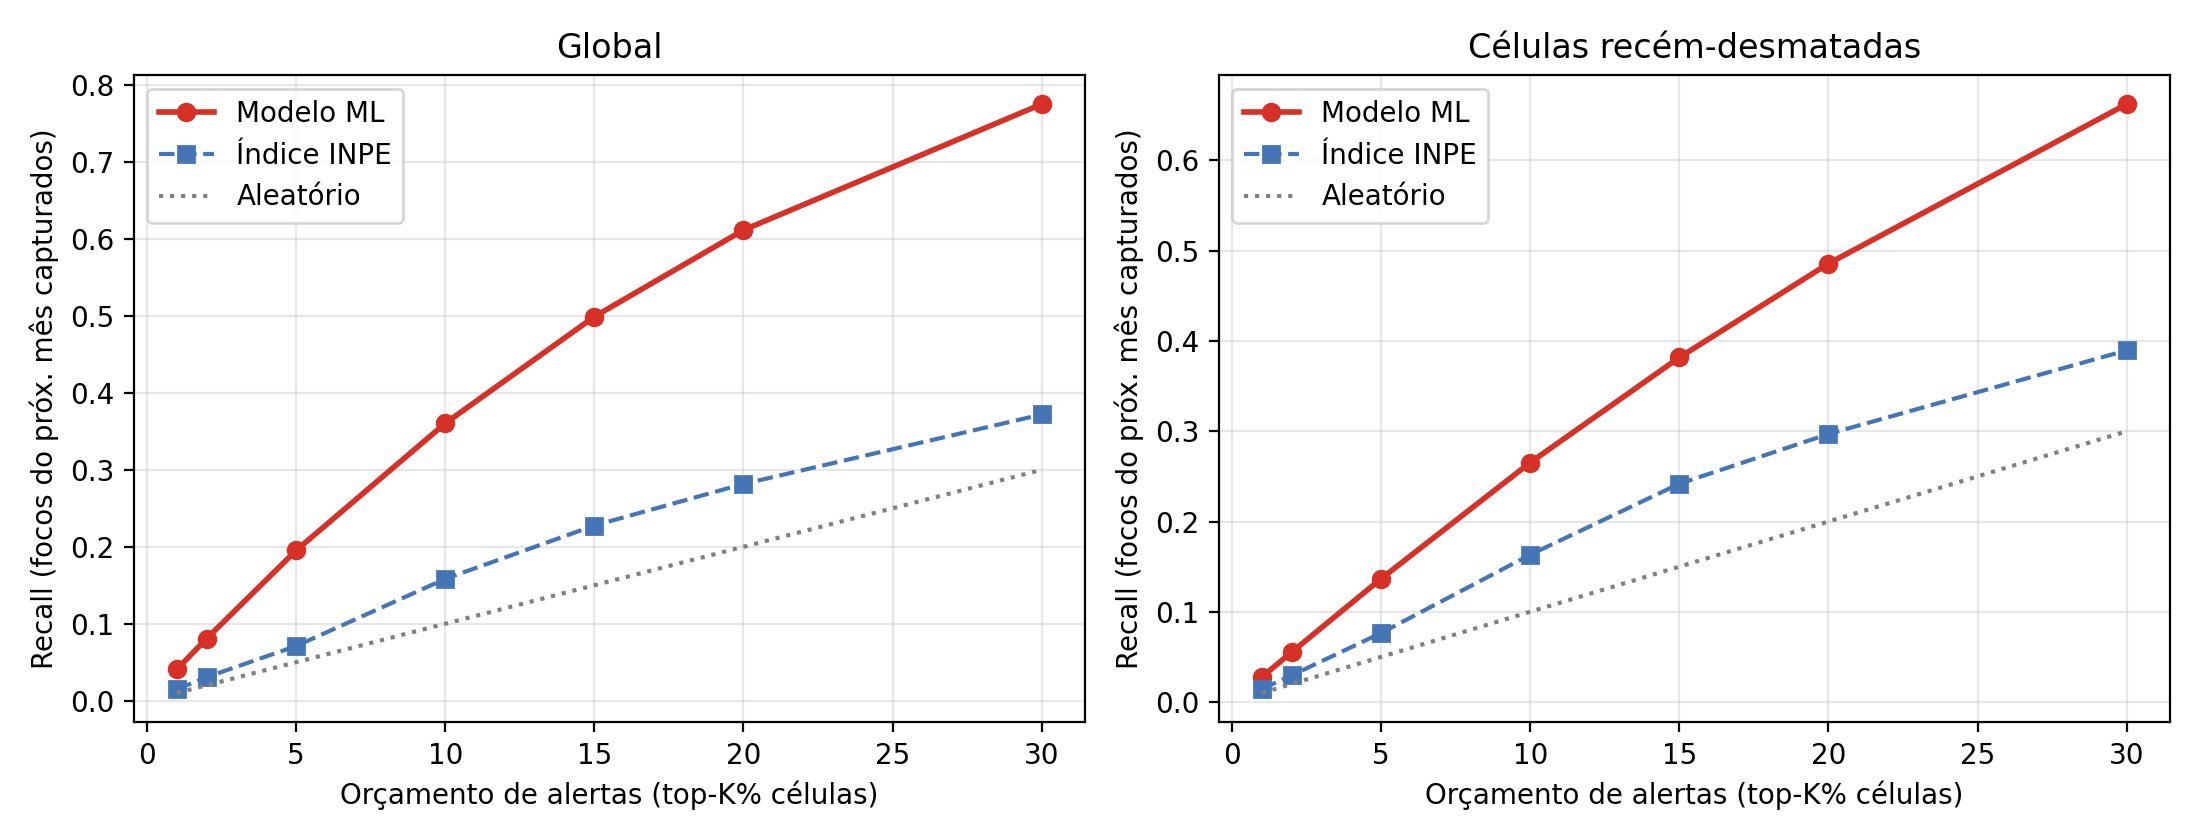
\includegraphics[width=\textwidth]{modelos/relatorios/avaliacao_operacional_recall_k.png}
\caption{\emph{Recall@K} em função do orçamento de alertas (modelo ML vs.\ índice INPE vs.\ aleatório), global (esq.) e em células recém-desmatadas (dir.).}
\label{fig:oco_recallk}
\end{figure}

\paragraph{Horizonte de previsão.} Estendendo o alvo para \(t+2\) e \(t+3\) meses, o
\emph{skill} permanece \textbf{estável} (PR-AUC \numlist{0,779;0,779;0,781} para \(t+1\),
\(t+2\), \(t+3\); Figura~\ref{fig:oco_horizonte}), sem o decaimento típico. Isso confirma
que a ocorrência mensal de fogo é governada por componentes \emph{lentos} (sazonalidade,
histórico de fogo, desmatamento), e não por dinâmica meteorológica de curto prazo ---
um resultado operacionalmente favorável, pois fornece \textbf{até um trimestre de
antecedência} sem perda de desempenho. A contrapartida honesta é que o modelo captura o
regime sazonal/persistente, não a dinâmica sub-mensal; previsões em escala mais fina
exigiriam outra formulação.

\begin{figure}[h]
\centering
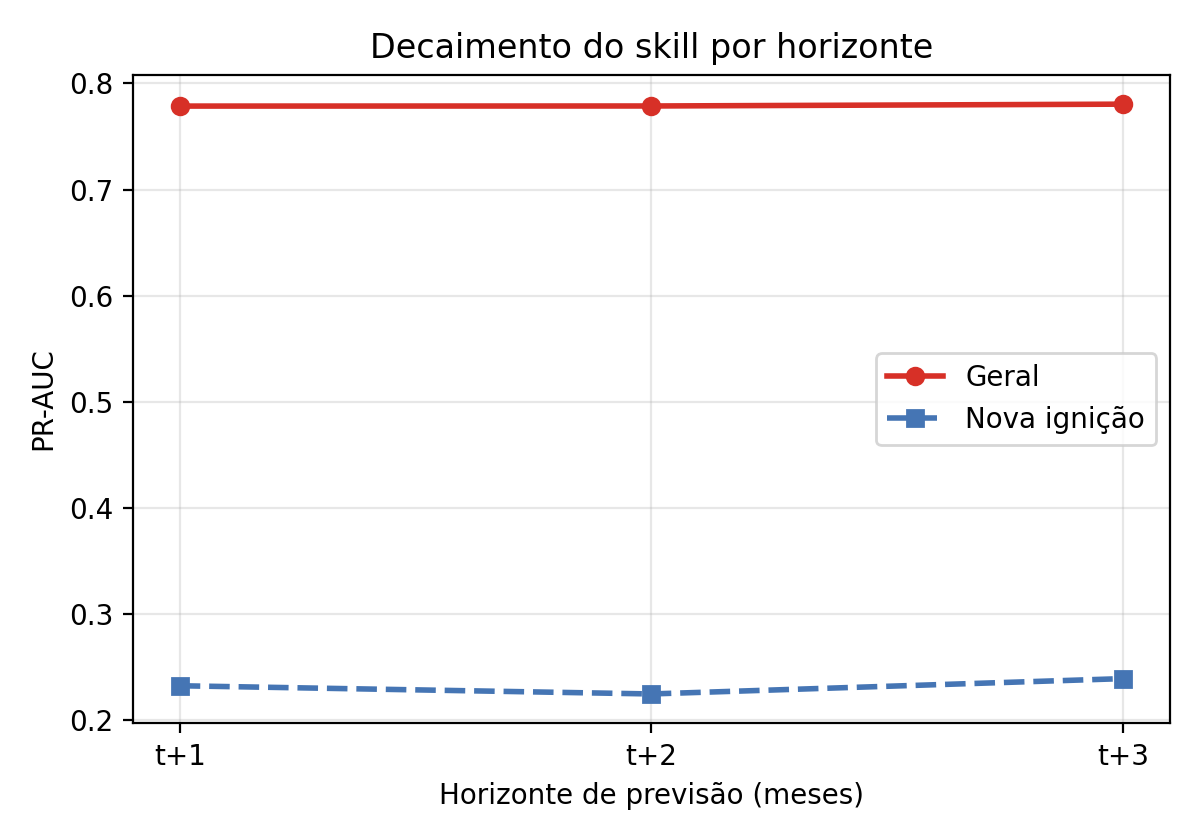
\includegraphics[width=0.6\textwidth]{modelos/relatorios/avaliacao_horizonte.png}
\caption{Decaimento do \emph{skill} (PR-AUC) por horizonte de previsão (\(t+1\) a \(t+3\) meses): estável, geral e na nova ignição.}
\label{fig:oco_horizonte}
\end{figure}

\section{Integração ao produto}
\label{sec:oco_produto}

O modelo final (base + desmatamento) foi serializado, calibrado por \emph{conformal}
(cobertura \num{0,900}) e exposto como produto: uma previsão por célula de \(P(\text{fogo no
próximo mês})\) com rótulo conformal e \emph{drivers}, servida por aplicação \emph{Flask} com
mapa interativo, independente do aplicativo de \emph{nowcast}. Verificações de sanidade
conferem com a fenologia do fogo (p.ex.\ Roraima com alto risco em dezembro; sul do Pará
baixo em dezembro, cuja estação de fogo é julho--outubro).

\section{Síntese}
\label{sec:oco_sintese}

Os experimentos, sob validação honesta, sustentam uma tese coesa: (i) na escala
mensal/\SI{0,25}{\degree}, a ocorrência de fogo é dominada por persistência espaço-temporal e
sazonalidade, o que torna redundantes a reanálise meteorológica (e o FWI) e a acessibilidade
estática; (ii) o modelo de ML \emph{supera} os índices físicos operacionais na previsão de
fogo observado; (iii) o gargalo é a \textbf{nova ignição}, e o único sinal útil ali é o
\textbf{desmatamento recente}, reposicionando o alerta precoce como, em primeira ordem, um
problema de detecção de fronteira de desmatamento; (iv) a incerteza é quantificável com
garantia estatística. A reformulação eleva o trabalho de ``reprodução de um índice'' para
``previsão de fogo observado validada contra a realidade e contra o índice físico'', com um
teto de desempenho honestamente caracterizado.



\chapter{Conclusão}
\label{cap:conclusao}

Este trabalho desenvolveu e validou um sistema de \textbf{previsão da ocorrência de fogo observado} na Amazônia Legal, a partir de dados do Programa Queimadas/INPE~\cite{INPE24} (2014--2023), com apoio de reanálise climática NASA POWER~\cite{nasapower}, detecções em tempo real NASA FIRMS~\cite{nasafirms}, dados de desmatamento PRODES/DETER e o \emph{shapefile} oficial do IBGE~\cite{ibgeamazonia2024}. A formulação central foi precedida por um \textbf{estudo exploratório} (Apêndice~\ref{cap:resultados}) que classificava o índice de Risco de Fogo do INPE em faixas de severidade; a constatação de que esse alvo era a \emph{saída de outro modelo} (circularidade metodológica) e de que a base era \emph{presence-only} (sem exemplos de não-fogo) motivou a reformulação aqui consolidada. Os principais achados são os seguintes.

\paragraph{1. Previsão de fogo observado, validada sem vazamento.} Reformulado o problema para \textbf{prever a ocorrência de foco no mês seguinte} (\(t+1\)) sobre uma grade de \SI{0,25}{\degree}, com classe negativa real e \emph{features} estritamente causais, o modelo (\emph{Histogram-based Gradient Boosting}~\cite{friedman2001greedy}) atingiu \textbf{\num{0,777} de PR-AUC} na validação temporal em bloco (\emph{rolling-origin}) e \textbf{\num{0,759}} na validação espacial (\emph{leave-region-out})~\cite{roberts2017cv}, superando com folga as linhas de base de persistência (\num{0,449}) e climatologia (\num{0,715}). Na validação espacial, a climatologia colapsa ao prever regiões nunca vistas enquanto o modelo se mantém --- indício de \emph{generalização} da dinâmica, e não de memorização da taxa-base local.

\paragraph{2. O aprendizado de máquina supera os índices físicos operacionais.} No \emph{benchmark} sobre fogo observado, medido nas mesmas amostras, o modelo (\num{0,858}) supera tanto o \emph{Fire Weather Index} canadense (\num{0,608})~\cite{vanwagner1985fwi} quanto o índice Risco de Fogo do INPE (\num{0,398}). Esse é o resultado que sustenta a tese: o modelo \textbf{agrega valor} sobre o índice físico que o estudo exploratório apenas reproduzia.

\paragraph{3. A nova ignição é o gargalo, e o desmatamento recente é o seu principal sinal.} A análise estratificada revela que o modelo é excelente onde o fogo \emph{recorre} (PR-AUC \num{0,805}) e difícil onde o fogo é \emph{novo} (PR-AUC \(\approx\)\num{0,23}) --- justamente o caso crítico para o alerta precoce. Entre as covariáveis testadas, apenas o \textbf{desmatamento recente} (PRODES anual e DETER mensal, resultados convergentes) agrega valor não-trivial nesse regime (\(\approx +\num{0,025}\) PR-AUC), confirmando o mecanismo causal de que o desmatamento \emph{precede} a primeira queimada de uma célula, coerente com a natureza majoritariamente antrópica do fogo amazônico~\cite{aragao2018amazon}. Clima (inclusive o FWI) e acessibilidade estática mostraram-se \emph{redundantes} frente ao histórico de fogo.

\paragraph{4. Incerteza calibrada e robustez ao algoritmo.} A \emph{conformal prediction}~\cite{sadinle2019lac} entrega cobertura empírica de \SI{88,8}{\percent}, distinguindo predições confiantes de ambíguas com garantia estatística. A comparação entre famílias de modelo com intervalos de confiança (\emph{cluster bootstrap} por célula) mostra que os \emph{ensembles} de árvore são estatisticamente equivalentes entre si e superam a regressão logística --- os achados \emph{não dependem} do algoritmo escolhido.

\paragraph{5. Rótulo validado contra fonte independente.} O rótulo (focos do INPE) foi confrontado com a área queimada do MapBiomas Fogo~\cite{mapbiomasfogo}: forte concordância interanual intra-estado (Spearman \(\approx\)\num{0,81}) e, no nível \emph{célula a célula}, concordância de \SI{78}{\percent} com revocação \num{0,90}. A ocorrência binária de fogo é, portanto, corroborada por um produto de modalidade distinta (cicatriz de área queimada).

\paragraph{6. Produto operacional e reprodutibilidade.} O modelo final foi serializado com os limiares conformais e serve, por uma \textbf{aplicação web interativa} (\emph{Flask} + \emph{Folium}~\cite{folium} + \emph{Leaflet}~\cite{leafletjs}), a probabilidade de fogo por célula no próximo mês, com rótulo de confiança e \emph{drivers} associados. Métricas, hiperparâmetros e metadados de \emph{split} ficam persistidos em JSON versionado, e o \emph{pipeline} é reexecutável por \emph{scripts} modulares --- reprodutibilidade tratada como requisito não funcional.

\paragraph{7. Estudo exploratório (baseline).} A primeira abordagem --- classificar o índice do INPE em três faixas --- alcançou \SI{84,61}{\percent} de acurácia em \emph{hold-out} aleatório, mas a própria validação temporal estrita expôs sua fragilidade (queda para \SI{70,13}{\percent}~\cite{bergmeir2012cv}) e, sobretudo, a circularidade do alvo. Documentada no Apêndice~\ref{cap:resultados}, ela cumpriu o papel de \emph{motivar} a reformulação central deste trabalho --- incluindo o estudo de caso Pium--TO, em que o índice do INPE indicava risco baixo num evento de fogo real confirmado pelo CENSIPAM.

\section{Limitações reconhecidas}
\label{sec:conclusao_limitacoes}

\begin{enumerate}
  \item \textbf{Granularidade mensal e espacial de \SI{0,25}{\degree}.} Picos diários de tempo seco e a dinâmica sub-mensal do fogo são diluídos nessa resolução; a hipótese de que a meteorologia passe a importar em escala sub-mensal não foi testada e permanece em aberto.

  \item \textbf{Domínio restrito a células propensas a fogo.} O modelo responde ``dada uma célula que já queimou na década, haverá fogo no próximo mês?'', não cobrindo o interior de floresta densa intacta --- restrição de domínio assumida para evitar o problema trivial de prever ausência de fogo onde ele praticamente nunca ocorre.

  \item \textbf{Teto da nova ignição (\(\approx\)\num{0,23} PR-AUC).} Esgotadas as dimensões do desmatamento (PRODES anual, DETER mensal, idade, estoque e fronteira), o ganho satura; parte da ignição é provavelmente \emph{irredutível} (decisão humana estocástica) ou exigiria dados de outra natureza (transição de uso do solo classe a classe, variáveis socioeconômicas).

  \item \textbf{Definição da classe negativa e cobertura climática.} A classe negativa foi construída com todos os \emph{cell-months} sem foco no domínio --- escolha que fixa a prevalência e deve ser reportada explicitamente; o clima das ausências vem de climatologia local (a reanálise gridada por célula-mês é melhoria em aberto), embora experimentos controlados tenham mostrado o sinal climático \emph{redundante} nessa escala.

  \item \textbf{Rótulo via focos do INPE.} Validado contra a área queimada do MapBiomas Fogo no nível estado/ano (Spearman \(\approx\)\num{0,81}) e \emph{célula a célula} até 2020 (concordância \SI{78}{\percent}, revocação \num{0,90}); resta estender a auditoria à resolução mensal e aos anos recentes (2021--2024).

  \item \textbf{Sem busca de hiperparâmetros por família.} As famílias foram comparadas com intervalos de confiança de \SI{95}{\percent} (equivalência estatística entre \emph{ensembles} de árvore), mas um \emph{tuning} dedicado por família (p.ex.\ Optuna) poderia render ganhos marginais.

  \item \textbf{Limitações do estudo exploratório (\emph{baseline}).} A abordagem inicial de classificação do índice do INPE herda vazamento temporal nas janelas móveis, base \emph{presence-only} e alvo circular; essas limitações estão documentadas no Apêndice~\ref{cap:resultados} e foram, precisamente, o que motivou a reformulação central.
\end{enumerate}

\section{Trabalhos futuros}
\label{sec:conclusao_futuros}

As direções de maior retorno para evoluir o sistema de previsão de ocorrência, priorizando o regime crítico da nova ignição, são:

\begin{enumerate}
  \item \textbf{Granularidade sub-mensal.} Testar se, em escala diária ou semanal, a meteorologia (FWI, VPD) recupera o poder preditivo que a agregação mensal dilui --- a hipótese mais direta para elevar o teto de desempenho.

  \item \textbf{Modelos espaço-temporais profundos} (ConvLSTM/U-Net ou \emph{graph neural networks} no estilo \emph{FireCastNet}~\cite{karasante2025firecastnet}) para capturar a propagação entre células vizinhas, ausente na formulação tabular.

  \item \textbf{Drivers antrópicos adicionais na nova ignição.} Transição de uso do solo classe a classe (MapBiomas), densidade de estradas e de frentes de desmatamento, e variáveis socioeconômicas --- as fontes mais promissoras para superar o teto de \(\approx\)\num{0,23} PR-AUC da nova ignição.

  \item \textbf{Validação célula a célula em escala mensal e anos recentes} --- a concordância com o MapBiomas Fogo~\cite{mapbiomasfogo} usou rasters anuais até 2020; estendê-la a 2021--2024 e à resolução mensal refinaria a auditoria de omissão/comissão dos focos.

  \item \textbf{Variáveis dinâmicas de combustível} --- NDVI/EVI MODIS e umidade do solo (SMAP) via Google Earth Engine, capturando o estado da vegetação que a climatologia não expressa.

  \item \textbf{Reanálise climática gridada completa} (ERA5 ou NASA POWER por célula-mês para todas as células), fechando a lacuna de cobertura climática das ausências e permitindo reavaliar o sinal meteorológico sem viés de amostragem.

  \item \textbf{Conformal prediction adaptado à dependência espaço-temporal}, para restaurar a garantia de cobertura sob quebra de \emph{exchangeability} inerente à autocorrelação da grade.

  \item \textbf{Extensão do domínio para além das células propensas}, com amostragem de \emph{background} principiada, ampliando a cobertura do sistema para o interior de floresta.
\end{enumerate}

\section{Considerações finais}
\label{sec:conclusao_consideracoes}

A revisão abrangente da literatura, descrita no Capítulo~2, evidenciou a complexidade do fenômeno das queimadas na Amazônia, ressaltando sua amplitude ambiental, social e econômica. Os resultados experimentais sustentam que ferramentas modernas de aprendizado de máquina, quando o problema é formulado como \textbf{previsão de fogo observado} e avaliado com validação honesta, representam contribuição relevante para o monitoramento da Amazônia Legal --- superando os índices físicos que operam hoje como referência.

O principal avanço científico do trabalho está em reposicionar o problema de ``reproduzir um índice'' para ``\textbf{prever o fenômeno observado e validá-lo contra a realidade}''. Sob validação espaço-temporal em bloco, o modelo alcança PR-AUC de \num{0,777} (temporal) e \num{0,759} (espacial) e \emph{supera} tanto o \emph{Fire Weather Index} canadense (\num{0,608}) quanto o Risco de Fogo do INPE (\num{0,398}) na previsão de fogo observado, com incerteza quantificada de forma calibrada. Mais do que o número agregado, a experimentação controlada identificou \emph{onde} e \emph{por quê} o sistema funciona: a \textbf{nova ignição} é o gargalo operacional, e o \textbf{desmatamento recente} --- não a meteorologia --- é o seu principal sinal preditivo, reposicionando o alerta precoce de fogo na Amazônia como, em primeira ordem, um problema de detecção da fronteira de desmatamento. A abordagem inicial de classificação do índice do INPE, que atingiu \SI{84,61}{\percent} de acurácia mas cujo alvo circular e base \emph{presence-only} comprometiam a interpretação, é preservada no Apêndice~\ref{cap:resultados} como o \emph{baseline} exploratório que motivou essa reorientação. Como continuidade natural, destacam-se a granularidade sub-mensal, a validação \emph{célula a célula} contra o MapBiomas Fogo em anos recentes e a adoção de modelos espaço-temporais profundos, conforme detalhado na Seção~\ref{sec:conclusao_futuros}.


\backmatter
\singlespacing
% ----------------------------------------------------------------------------------------------------- %
\bibliography{references}

\appendix
\onehalfspacing

% Estudo exploratório (antigo Cap. 5): classificação do índice de risco do INPE.
% Rebaixado a apêndice — o alvo era a saída de outro modelo (circularidade);
% a contribuição central é a previsão de fogo observado (Cap. de Previsão de Ocorrência).
% ============================================================================
% AP_estudo_exploratorio.tex
% Movido do antigo Capítulo 5 (Resultados) — abordagem exploratória de
% classificação do índice de Risco de Fogo do INPE. Rebaixado a apêndice:
% o alvo era a saída de outro modelo (circularidade metodológica), o que
% motivou a reformulação central para previsão de fogo OBSERVADO (Cap. de
% Previsão de Ocorrência). Mantido como material complementar / baseline.
% Inclui (Seção A.1) a metodologia própria do baseline, antes no Cap. 4.
% ============================================================================
\chapter{Estudo Exploratório: Classificação do Índice de Risco de Fogo (baseline)}
\label{cap:resultados}

Este apêndice documenta a abordagem exploratória inicial do trabalho: a classificação supervisionada do índice de Risco de Fogo do INPE em três faixas de severidade. Ela é preservada como \emph{baseline} porque a análise de suas fragilidades --- alvo que é a saída de outro modelo, base \emph{presence-only} e vazamento temporal --- motivou a reformulação central apresentada nos Capítulos~\ref{cap:metodologia} e~\ref{cap:ocorrencia}. A Seção~\ref{sec:ap_metodologia} descreve a metodologia própria dessa abordagem; as seções seguintes reportam o conjunto de dados e o protocolo (Seção~\ref{sec:res_dataset}), o comparativo das oito abordagens (Seção~\ref{sec:res_comparativo}), o modelo final (Seção~\ref{sec:res_modelo_final}), a interpretabilidade (Seção~\ref{sec:res_interpretabilidade}), a validação temporal estrita (Seção~\ref{sec:res_temporal}), o ajuste de limiares (Seção~\ref{sec:res_threshold}), a evolução do \emph{pipeline} (Seção~\ref{sec:res_evolucao}), a validação via aplicação web (Seção~\ref{sec:res_app}) e o estudo de caso Pium--TO (Seção~\ref{sec:res_estudo_caso_pium}).

\section{Metodologia do estudo exploratório}
\label{sec:ap_metodologia}

Esta seção documenta os procedimentos específicos da abordagem exploratória. A coleta dos focos do Programa Queimadas é comum a todo o trabalho e está descrita na Seção~\ref{sec:metod_coleta}; aqui constam apenas as etapas próprias da classificação do índice de Risco de Fogo do INPE.

\subsection{Pré-processamento e definição do alvo}
\label{sec:metodologia_pre_processamento}

Cada linha da base corresponde a um foco de calor (\num{933954} registros brutos, 2014--2023). A limpeza removeu as colunas sem valor preditivo (\texttt{Satelite}, \texttt{Pais}, \texttt{Bioma}), substituiu o sentinela \texttt{-999} por valor ausente e descartou os focos sem \texttt{RiscoFogo} válido. O alvo, \texttt{RiscoClassificado}, é a discretização do índice \texttt{RiscoFogo} do INPE (escala 0--1) em três faixas por limiares semânticos: \emph{Baixo} (\(< 0{,}50\)), \emph{Moderado} (\(0{,}50\)--\(0{,}80\)) e \emph{Muito Alto} (\(\geq 0{,}80\)); os limiares ficam persistidos em \texttt{modelos/risk\_thresholds.json}.

As variáveis preditoras originais são numéricas (\texttt{DiaSemChuva}, \texttt{Precipitacao}, \texttt{Latitude}, \texttt{Longitude}, \texttt{FRP}, \texttt{Ano}, \texttt{Mes}, \texttt{Dia}, \texttt{Hora}) e categóricas (\texttt{Estado}, \texttt{Municipio}). Um \texttt{ColumnTransformer} aplica imputação pela mediana e \texttt{StandardScaler} às numéricas, e imputação pela moda e \texttt{OneHotEncoder} às categóricas. Note-se que \texttt{DiaSemChuva} e \texttt{Precipitacao} são insumos do próprio índice do INPE --- a circularidade discutida na Seção~\ref{sec:oco_motivacao}.

\paragraph{Enriquecimento com umidade relativa (NASA POWER).}
\label{subsec:metod_apis_externas}
A reanálise NASA POWER~\cite{nasapower} foi consultada para extrair a umidade relativa a \SI{2}{m} (RH2M) no local e na data de cada foco, via \texttt{scripts/enriquecer\_dados\_umidade.py}, com \emph{cache} em disco e respeito ao limite de taxa da API. Pela latência do enriquecimento total (\(\approx 16\)~dias para \num{755711} requisições únicas), \num{170465} registros foram efetivamente enriquecidos (\(\approx \SI{18,3}{\percent}\) da base) e os demais foram imputados por \emph{pseudo-labeling} (Seção~\ref{sec:metodologia_pseudo_label}).

\subsubsection{Engenharia de \emph{features} físico-climáticas (Tier 1)}
\label{subsec:metod_features_tier1}

Em complemento às nove \emph{features} originais do Programa Queimadas, foram derivadas \textbf{24~\emph{features} físico-climáticas avançadas} (Tier~1), agrupadas em sete camadas (implementação em \texttt{scripts/features\_avancadas.py}). A Tabela~\ref{tab:metod_tier1} resume as camadas com a justificativa bibliográfica de cada uma.

\begin{table}[h]
\centering
\caption{Camadas Tier~1 de \emph{features} físico-climáticas adicionadas ao \emph{dataset}.}
\label{tab:metod_tier1}
\small
\begin{tabular}{clp{6cm}l}
\toprule
\textbf{\#} & \textbf{Camada} & \textbf{\emph{Features}} & \textbf{Justificativa} \\
\midrule
1 & Médias móveis estendidas & \texttt{Precipitacao\_ma14/30/90}, \texttt{DiaSemChuva\_ma14/30/90} & \emph{Fuel moisture lag}~\cite{seager2015climatology} \\
2 & Precipitação acumulada & \texttt{Precipitacao\_acum\_30/90/180/365d} & \cite{seager2015climatology} \\
3 & SPI & \texttt{SPI\_1m}, \texttt{SPI\_3m}, \texttt{SPI\_6m} & \cite{mckee1993spi,npjhazards2025fire} \\
4 & Anomalia de precipitação & \texttt{Anomalia\_Precipitacao}, \texttt{Anomalia\_Precipitacao\_rel} & \cite{forests2024cerradoamazon} \\
5 & KBDI, VPD, De Martonne & \texttt{Temp\_Climatologica}, \texttt{KBDI\_proxy}, \texttt{VPD\_proxy}, \texttt{Aridez\_DeMartonne} & \cite{keetch1968drought,seager2015climatology,demartonne1926aridity,forests2024cerradoamazon} \\
6 & Histórico estendido de incêndios & \texttt{Incendios\_Ultimos\_90/180/365\_Dias}, \texttt{Media\_FRP\_Celula\_30d} & \cite{cheerala2025probabilistic} \\
7 & Estação seca acumulada & \texttt{Dias\_Secos\_90d} & \emph{Canadian Drought Code} (FWI) \\
\bottomrule
\end{tabular}
\end{table}

A granularidade espacial das camadas 1, 2, 6, 7 e do SPI usa \textbf{células de \(0{,}25^\circ\)} (\(\approx \SI{27}{\km}\)), o que evita colapso das janelas temporais que ocorreria com agrupamento por coordenadas literais (cada foco é um ponto único). A \emph{climatologia} de temperatura provém de uma tabela estática de médias mensais por estado, aproximada a partir das Normais Climatológicas do INMET 1981--2010~\cite{inmetnormais}. O CSV final \texttt{base\_de\_dados\_enriquecido.csv} contém \num{924306} linhas e 46~colunas, com tempo total de geração de \(\approx \SI{40}{\second}\) sobre os \num{933954} registros brutos.

\subsubsection{Calibração de probabilidades}
\label{subsec:metod_calibracao}

A predição padrão dos modelos retorna escores não-calibrados. Para que a saída do modelo seja interpretável como ``\(P(\text{classe} \mid \text{features}) = 0{,}73\)'', aplicou-se \texttt{CalibratedClassifierCV(method='isotonic', cv=3)} aos modelos do \emph{ensemble} final. A calibração isotônica~\cite{zadrozny2002transforming} ajusta uma função monotônica não-paramétrica entre escores brutos e probabilidades empíricas, sem assumir forma sigmoide --- escolha defensável dada a natureza não linear dos GBMs envolvidos.

\subsection{Treinamento dos Modelos de Previsão}
\label{sec:metod_treinamento}

Neste ponto, todos os algoritmos utilizaram a mesma \emph{pipeline}, garantindo que os dados fossem preparados de maneira consistente para os processos de treinamento e teste. O objetivo foi comparar os resultados gerados por cada modelo em um cenário base comum, assegurando que não houvesse qualquer tipo de viés, exceto aqueles originados exclusivamente pelo desempenho de cada algoritmo. A partir de um conjunto de dados previamente processados, foram aplicados algoritmos de classificação para identificar as áreas mais suscetíveis a queimadas com base em atributos climáticos, topográficos e históricos.

O treinamento dos modelos foi realizado utilizando a biblioteca \texttt{scikit-learn}~\cite{pedregosa2011scikit}, complementada por \texttt{xgboost}~\cite{chen2016xgboost}, \texttt{lightgbm}~\cite{ke2017lightgbm}, \texttt{catboost}~\cite{prokhorenkova2018catboost}, \texttt{optuna}~\cite{akiba2019optuna} e \texttt{imbalanced-learn}~\cite{lemaitre2017imbalanced}.

\subsubsection{Divisão dos dados e construção do \emph{pipeline}}

O conjunto de dados foi dividido em treino (\SI{80}{\percent}) e teste (\SI{20}{\percent}) utilizando \texttt{train\_test\_split(stratify=y, random\_state=42)}, preservando a distribuição das três classes em ambos os subconjuntos. Os metadados do \emph{split} (\texttt{random\_state}, \texttt{test\_size}, estratificação) ficam persistidos em \texttt{modelos/split\_metadata.json} para garantir reprodutibilidade. O conjunto de teste contém \num{184862} observações.

O \emph{pipeline} de processamento foi implementado via \texttt{sklearn.pipeline.Pipeline}, composto por:

\begin{enumerate}
  \item \texttt{ColumnTransformer} --- aplica \texttt{SimpleImputer(strategy='median')} + \texttt{StandardScaler} às \emph{features} numéricas e \texttt{SimpleImputer(strategy='most\_frequent')} + \texttt{OneHotEncoder} às \emph{features} categóricas.
  \item \texttt{CalibratedClassifierCV(method='isotonic', cv=3)} --- envolve o classificador final para garantir calibração das probabilidades.
  \item \textbf{Estimador} --- variável conforme o modelo avaliado.
\end{enumerate}

\subsubsection{Modelos avaliados}

Oito abordagens foram comparadas no mesmo conjunto de treino/teste:

\begin{enumerate}
  \item \textbf{Regressão Logística balanceada} --- \texttt{class\_weight='balanced'}, hiperparâmetros otimizados via Optuna (\texttt{C=12.43, max\_iter=4768}).
  \item \textbf{SGDClassifier} --- perda logística, \emph{online learning}; \emph{baseline} simples original do projeto.
  \item \textbf{Random Forest com SMOTE}~\cite{chawla2002smote} --- variante para tratamento de desbalanceamento amostral.
  \item \textbf{Random Forest balanceado otimizado}~\cite{breiman2001random} --- \texttt{class\_weight='balanced'}, Optuna (15 \emph{trials}, 3-\emph{fold} CV, \(\text{F}_1\)-macro): \texttt{n\_estimators=346, max\_depth=25, min\_samples\_split=3, max\_features='sqrt'}.
  \item \textbf{XGBoost otimizado}~\cite{chen2016xgboost} --- Optuna (15 \emph{trials}, 3-\emph{fold} CV, \(\text{F}_1\)-macro, \emph{subsample} de 250\,k): \texttt{n\_estimators=346, learning\_rate=0.073, max\_depth=14, subsample=0.74, colsample\_bytree=0.93, gamma=0.03}.
  \item \textbf{LightGBM otimizado}~\cite{ke2017lightgbm} --- Optuna (15 \emph{trials}, \(\text{F}_1\)-macro): \texttt{n\_estimators=683, learning\_rate=0.066, num\_leaves=204, min\_child\_samples=24, subsample=0.78, colsample\_bytree=0.77}.
  \item \textbf{CatBoost}~\cite{prokhorenkova2018catboost} --- \texttt{iterations=1000, learning\_rate=0.05, depth=8, auto\_class\_weights='Balanced'}.
  \item \textbf{Ensemble Voting Soft} --- média das probabilidades calibradas de RF, LR, XGBoost, LightGBM e CatBoost.
  \item \textbf{Ensemble Stacking}~\cite{wolpert1992stacked} --- RF, LR, XGBoost, LightGBM e CatBoost como \emph{base learners}; \texttt{GradientBoostingClassifier}~\cite{friedman2001greedy} como meta-classificador (\texttt{n\_estimators=200, max\_depth=3, learning\_rate=0.1}). Esta é a configuração final adotada (\texttt{ensemble\_stacking\_gbm}).
\end{enumerate}

Todos os modelos foram salvos via \texttt{joblib.dump()} em arquivos \texttt{.pkl} no diretório \texttt{modelos/}. Os hiperparâmetros otimizados via Optuna ficam persistidos em \texttt{modelos/relatorios/optuna\_*.json}.

\subsubsection{Tempo de treinamento}

A Tabela~\ref{tab:metod_tempos} apresenta o tempo de treinamento de cada abordagem em ambiente CPU com 8~núcleos e \SI{16}{\giga\byte} de RAM.

\begin{table}[h]
\centering
\caption{Tempo de treinamento por modelo.}
\label{tab:metod_tempos}
\small
\begin{tabular}{lr}
\toprule
\textbf{Modelo} & \textbf{Tempo (segundos)} \\
\midrule
Regressão Logística balanceada & 25 \\
SGDClassifier                  & 8 \\
Random Forest + SMOTE          & 480 \\
Random Forest balanceado (Optuna) & 1\,100 \\
XGBoost (Optuna, 250k \emph{subsample}) & 540 \\
LightGBM (Optuna, 250k \emph{subsample}) & 290 \\
CatBoost                       & 410 \\
Ensemble Voting Soft           & 2\,360 (soma dos \emph{base learners} + agregação) \\
\textbf{Ensemble Stacking GBM} & \textbf{5\,100 (\(\approx\) 85~min)} \\
\bottomrule
\end{tabular}
\end{table}

\subsection{Avaliação dos Modelos de Previsão}
\label{sec:metod_avaliacao}

A avaliação foi realizada sobre o conjunto de teste de \num{184862} observações. Quatro componentes complementares foram considerados: métricas tradicionais (Seção~\ref{subsec:metod_metricas}), interpretabilidade (Seção~\ref{subsec:metod_interpretabilidade}), ajuste multi-classe de limiares (Seção~\ref{subsec:metod_thresholds}) e validação temporal estrita (Seção~\ref{subsec:metod_validacao_temporal}).

\subsubsection{Métricas utilizadas}
\label{subsec:metod_metricas}

\begin{itemize}
  \item \textbf{Acurácia global} --- fração de predições corretas (\texttt{accuracy\_score}).
  \item \textbf{\(\text{F}_1\) por classe e \(\text{F}_1\)-macro} --- \texttt{f1\_score(average='macro')}. A \(\text{F}_1\)-macro é a média não ponderada entre as três classes; é a métrica primária por ser robusta a desbalanceamento.
  \item \textbf{Precisão e revocação por classe} --- via \texttt{classification\_report}.
  \item \textbf{Matriz de confusão normalizada} --- \texttt{confusion\_matrix(normalize='true')}.
  \item \textbf{Confiança média e distribuição} --- média e histograma de \(\max\) de \texttt{predict\_proba(X\_test)}.
  \item \textbf{Curva de calibração} --- \texttt{calibration\_curve}, para confirmar que a probabilidade predita corresponde à frequência empírica observada.
\end{itemize}

\subsubsection{Análise de interpretabilidade}
\label{subsec:metod_interpretabilidade}

Duas técnicas complementares são aplicadas para identificar as \emph{features} mais relevantes:

\paragraph{SHAP por classe via Random Forest leve \emph{proxy}~\cite{lundberg2017unified,lundberg2020local}.} O \texttt{TreeExplainer} aplicado ao \emph{Stacking GBM} final e ao RF Optuna produtivo demanda mais de \num{2}\,\text{GiB} por classe em CPU pós-OHE. Como solução cientificamente defensável~\cite{lundberg2020local}, treina-se um Random Forest \emph{compacto} (100 árvores, \texttt{max\_depth=12}, \texttt{class\_weight='balanced'}, \num{60000} amostras de treino) como \emph{proxy interpretativo}. O script \texttt{scripts/analise\_shap\_rf\_leve.py} aplica \texttt{shap.TreeExplainer} sobre 500 amostras de teste e exporta as importâncias médias absolutas por classe em \texttt{modelos/relatorios/shap\_per\_class.json}.

\paragraph{\emph{Permutation Importance}~\cite{breiman2001random,fisher2019all}.} Aplicada diretamente sobre o \texttt{ensemble\_stacking\_gbm} em produção (5\,000 amostras de teste, três repetições, \emph{seed}=42). Para cada \emph{feature}, calcula-se a queda em \(\text{F}_1\) por classe e em \(\text{F}_1\)-macro quando os valores são permutados aleatoriamente. Diferentemente da importância Gini/MDI, é \emph{model-agnostic} e \textbf{não tendenciosa} para \emph{features} de alta cardinalidade~\cite{strobl2007bias} --- característica relevante dado o OHE de \texttt{Municipio} (542 categorias). A saída fica em \texttt{modelos/relatorios/permutation\_importance\_por\_classe.json}.

\subsubsection{Ajuste multi-classe de limiares de decisão}
\label{subsec:metod_thresholds}

A predição padrão usa \texttt{argmax} sobre as probabilidades calibradas. Embora maximize \(P(\text{classe} \mid x)\), penaliza a classe \emph{Moderado} --- fronteira ambígua entre \emph{Baixo} e \emph{Muito Alto}~\cite{he2009learning}. O procedimento implementado em \texttt{scripts/ajustar\_threshold.py} varre uma grade de pares (\texttt{thr\_Moderado}, \texttt{thr\_Muito\_Alto}) \(\in \{0{,}30; 0{,}35; \ldots; 0{,}55\}^2\) (36 combinações), com critério primário \(\text{F}_1\)-macro e secundário \(\text{F}_1\)-Moderado. Os limiares finais são persistidos em \texttt{modelos/prediction\_thresholds.json} e aplicados em \emph{runtime} no aplicativo web via parâmetro \texttt{estrategia\_thresholds} do \emph{endpoint} \texttt{/api/predict}.

A lógica de decisão multi-classe em \emph{runtime} é:

\begin{verbatim}
se      P(Moderado)   >= thr_Moderado    -> classe = "Moderado"
senao se P(Muito Alto) >= thr_Muito_Alto -> classe = "Muito Alto"
senao                                    -> classe = "Baixo"
\end{verbatim}

\subsubsection{Validação temporal (\emph{rolling-origin})}
\label{subsec:metod_validacao_temporal}

Em complemento à validação no \emph{split} aleatório, foi implementado em \texttt{scripts/validacao\_temporal.py} um procedimento de \textbf{\emph{rolling-origin} por ano}~\cite{bergmeir2012cv}. Para cada ano \(Y \in \{2021, 2022, 2023\}\) (três últimos com massa suficiente), o modelo é treinado em \(\text{Ano} < Y\) (\emph{subsample} estratificado de \num{60000} amostras por \emph{fold} para o \emph{Stacking}, limite de memória do OHE denso de \texttt{Municipio}) e avaliado em \(\text{Ano} = Y\). Cobre o uso operacional realista: ``treine com o passado, prediga o ano seguinte''. O resultado é apresentado no Apêndice~\ref{cap:resultados}.

\subsection{Aplicação web interativa explicável}
\label{sec:metod_app_web}

Para tornar o modelo final utilizável e auditável por gestores ambientais, foi desenvolvida uma aplicação web (\texttt{scripts/app\_map\_interativo.py}) baseada em \emph{Flask} + \emph{Folium}~\cite{folium} + \emph{Leaflet}~\cite{leafletjs} que serve como interface explicável sobre o \emph{pipeline}. O usuário clica em qualquer ponto da Amazônia Legal e o sistema responde, em \(\approx 10\)--\SI{20}{\second}, com a predição classificada, acompanhada das 24~\emph{features} Tier~1 calculadas para o ponto, da explicação local das \emph{features} mais influentes e do contexto histórico comparativo.

\subsubsection{\emph{Pipeline} de predição pontual}

Como o aplicativo prediz \textbf{um único ponto isolado}, sem histórico temporal local, as \emph{features} Tier~1 que dependem de séries (SPI, acumulados longos, histórico estendido de focos) não podem ser calculadas em tempo real. Adota-se a estratégia de \textbf{\emph{lookup} espaço-sazonal} (\texttt{scripts/feature\_lookup.py}):

\begin{enumerate}
  \item Pré-cálculo das medianas das 24~\emph{features} Tier~1 do \emph{dataset} enriquecido, agregadas em três níveis de granularidade decrescente: \((\text{LatBin}~0{,}25^\circ, \text{LonBin}~0{,}25^\circ, \text{Mes})\), depois \((\text{Estado}, \text{Mes})\) e, por fim, \text{Mes} global.

  \item Para o ponto consultado, \emph{lookup} em cascata (do mais fino ao mais grosso) com tolerância de \(\pm 1\) célula.

  \item \emph{Features} físicas independentes de série temporal (\texttt{Temp\_Climatologica}, \texttt{KBDI\_proxy}, \texttt{VPD\_proxy}, \texttt{Aridez\_DeMartonne}, \texttt{Anomalia\_Precipitacao}) são recalculadas em tempo real com o clima NASA POWER atual e a climatologia local da precipitação --- o \emph{lookup} fornece apenas os ``blocos de construção'' históricos imutáveis.
\end{enumerate}

\subsubsection{Integração de dados em tempo real}

\begin{itemize}
  \item \textbf{Geocodificação reversa} via Nominatim/OpenStreetMap para extrair Estado e Município do clique.
  \item \textbf{Clima atual} via NASA POWER~\cite{nasapower} (precipitação, dias sem chuva, RH2M dos últimos 28~dias).
  \item \textbf{Focos ativos} via NASA FIRMS~\cite{nasafirms} para \texttt{FRP} dos últimos 7~dias no raio de \SI{10}{\km} do ponto.
\end{itemize}

\subsubsection{Explicabilidade local}

Em \emph{runtime}, \texttt{scripts/explainer.py} aproxima a contribuição de cada \emph{feature} como
\begin{equation}
\text{contrib}(f) = \text{importância}(f) \times \text{zscore}(f) \times \text{sinal\_físico}(f),
\end{equation}
onde \(\text{importância}(f)\) é carregada de \texttt{shap\_per\_class.json} (importância por classe predita, quando disponível) ou de \texttt{shap\_feature\_importance.json} (Gini global como \emph{fallback}); \(\text{zscore}(f)\) mede a anormalidade do valor no ponto em relação à distribuição global do \emph{dataset}; e \(\text{sinal\_físico}(f) \in \{-1, +1\}\) codifica o efeito esperado (por exemplo, \(+1\) para \texttt{Indice\_Seca}, \(-1\) para \texttt{Precipitacao\_ma90}). A predição é classificada como \emph{AUMENTA RISCO}, \emph{REDUZ RISCO} ou \emph{neutro}; o \emph{top-6 features} por \(|\text{contrib}|\) é exibido no painel lateral.

\subsubsection{Interface}

O \emph{front-end} é organizado em \textbf{seis \emph{cards}} dentro de um painel lateral de \num{420}\,px:

\begin{enumerate}
  \item \textbf{Previsão} --- \emph{badge} com a classe, barras de probabilidade por classe, métricas do modelo, fonte do clima, granularidade do \emph{lookup} e \emph{trace} da decisão (\emph{argmax} \emph{vs.}\ \emph{thresholds} calibrados).
  \item \textbf{Por que esse risco?} --- \emph{top-6 features} com valor, faixa típica (\(p_{10}\)--\(p_{90}\) da distribuição global), \emph{z-score} e direção do impacto.
  \item \textbf{Dados climáticos atuais} --- precipitação, dias sem chuva, umidade NASA, temperatura climatológica, estação, período do dia.
  \item \textbf{Índices de seca e aridez} --- Índice de Seca, SPI 1m/3m/6m, KBDI \emph{proxy}, Aridez De Martonne, VPD \emph{proxy}, Dias\_Secos\_90d.
  \item \textbf{Precipitação acumulada e anomalia} --- acumulados 30/90/180/365~dias com narrativa textual comparando precipitação atual e a média histórica do município/mês.
  \item \textbf{Histórico de focos} --- focos NASA FIRMS em 7/30/90/180/365~dias, dias desde o último foco, FRP médio/máximo 7d, FRP no ponto agora.
\end{enumerate}

O mapa estático (versão original da Seção 4.6 do TCC~II) permanece disponível como artefato \emph{batch} (\texttt{scripts/gerar\_mapa.py}).

\subsection{Imputação de \emph{Umidade} via \emph{pseudo-labeling}}
\label{sec:metodologia_pseudo_label}

Como discutido na Seção~\ref{subsec:metod_apis_externas}, a integração via NASA POWER produziu \num{170465} linhas com \texttt{Umidade} real (\(\approx \SI{18,3}{\percent}\) da base). Para mitigar essa cobertura parcial sem aguardar 13~dias adicionais de enriquecimento, foi implementada a estratégia de \textbf{\emph{pseudo-labeling}}~\cite{lee2013pseudo}, com precedente recente em imputação climática~\cite{lopezgarcia2024spatiotemporal}. O \emph{script} \texttt{scripts/pseudo\_label\_umidade.py} executa as etapas:

\begin{enumerate}
  \item Treina um \textbf{LightGBM regressor}~\cite{ke2017lightgbm} sobre os \(\approx \num{170000}\) registros com \texttt{Umidade} real, usando 15~\emph{features} (precipitação, dias sem chuva, lat/lon, sazonalidade cíclica \texttt{Mes\_sin/cos}, histórico de fogo) --- \emph{features} que existem para todas as linhas, com ou sem \texttt{Umidade} real.

  \item Avalia o erro real em \emph{holdout} 20\%: \textbf{RMSE = \SI{4,33}{\percent} RH, MAE = \SI{3,19}{\percent} RH, \(R^2 = 0{,}933\)}. O \(R^2\) alto é cientificamente justificável: a umidade tem alta autocorrelação espaço-sazonal com as \emph{features} usadas --- lat/lon definem o regime de monção, mês define a estação seca/chuvosa, precipitação recente define o estado higroscópico do ar.

  \item Refit no \SI{100}{\percent} dos \emph{labels} reais e imputa os \num{763489} registros sem \emph{label} (\emph{clip} [5, 100]\%).

  \item Salva o \emph{dataset} enriquecido em \texttt{base\_de\_dados\_umidade\_pseudo.csv} com coluna auxiliar \texttt{Umidade\_origem} \(\in\) \{\texttt{nasa\_power}, \texttt{pseudo\_label\_lgbm}\} para auditoria.
\end{enumerate}

\paragraph{Status no \emph{pipeline} final.} O \emph{dataset} \texttt{base\_de\_dados\_umidade\_pseudo.csv} está disponível mas \textbf{não é usado nos números finais reportados} no Apêndice~\ref{cap:resultados}. Razão: incluir \texttt{Umidade} (pseudo-rotulada ou real) exigiria retreino completo do \texttt{ensemble\_stacking\_gbm} (\(\approx \SI{85}{\minute}\) CPU) + revalidação das \emph{thresholds} + revalidação temporal --- fora do orçamento computacional desta entrega. O artefato fica registrado como \textbf{etapa preparatória} para a sequência natural do trabalho. Cautela registrada: \emph{pseudo-labels} devem ser interpretados considerando potencial viés de confirmação~\cite{arazo2020pseudo}.

\section{Conjunto de dados e protocolo de avaliação}
\label{sec:res_dataset}

Após a limpeza descrita na Seção~\ref{sec:metodologia_pre_processamento} e o enriquecimento físico-climático Tier~1 da Seção~\ref{subsec:metod_features_tier1}, o conjunto de dados final (\texttt{base\_de\_dados\_enriquecido.csv}) totaliza \textbf{\num{924306} observações}, com 44~\emph{features} numéricas e 4~\emph{features} categóricas (\texttt{Estado}, \texttt{Municipio}, \texttt{Estacao}, \texttt{Periodo\_Dia}). A divisão \texttt{train\_test\_split} (\texttt{test\_size=0.20}, \texttt{stratify=y}, \texttt{random\_state=42}) produz \(\approx \num{739444}\) observações de treino e \textbf{\num{184862}} de teste, com a distribuição estratificada das três classes preservada em ambos os conjuntos (Figura~\ref{fig:res_distribuicao}): \emph{Baixo} \(\approx \SI{36,6}{\percent}\); \emph{Moderado} \(\approx \SI{16,8}{\percent}\); \emph{Muito Alto} \(\approx \SI{46,6}{\percent}\). O \emph{seed} fixo e o metadado completo do \emph{split} ficam persistidos em \texttt{modelos/split\_metadata.json} para garantir reprodutibilidade.

\begin{figure}[h]
\centering
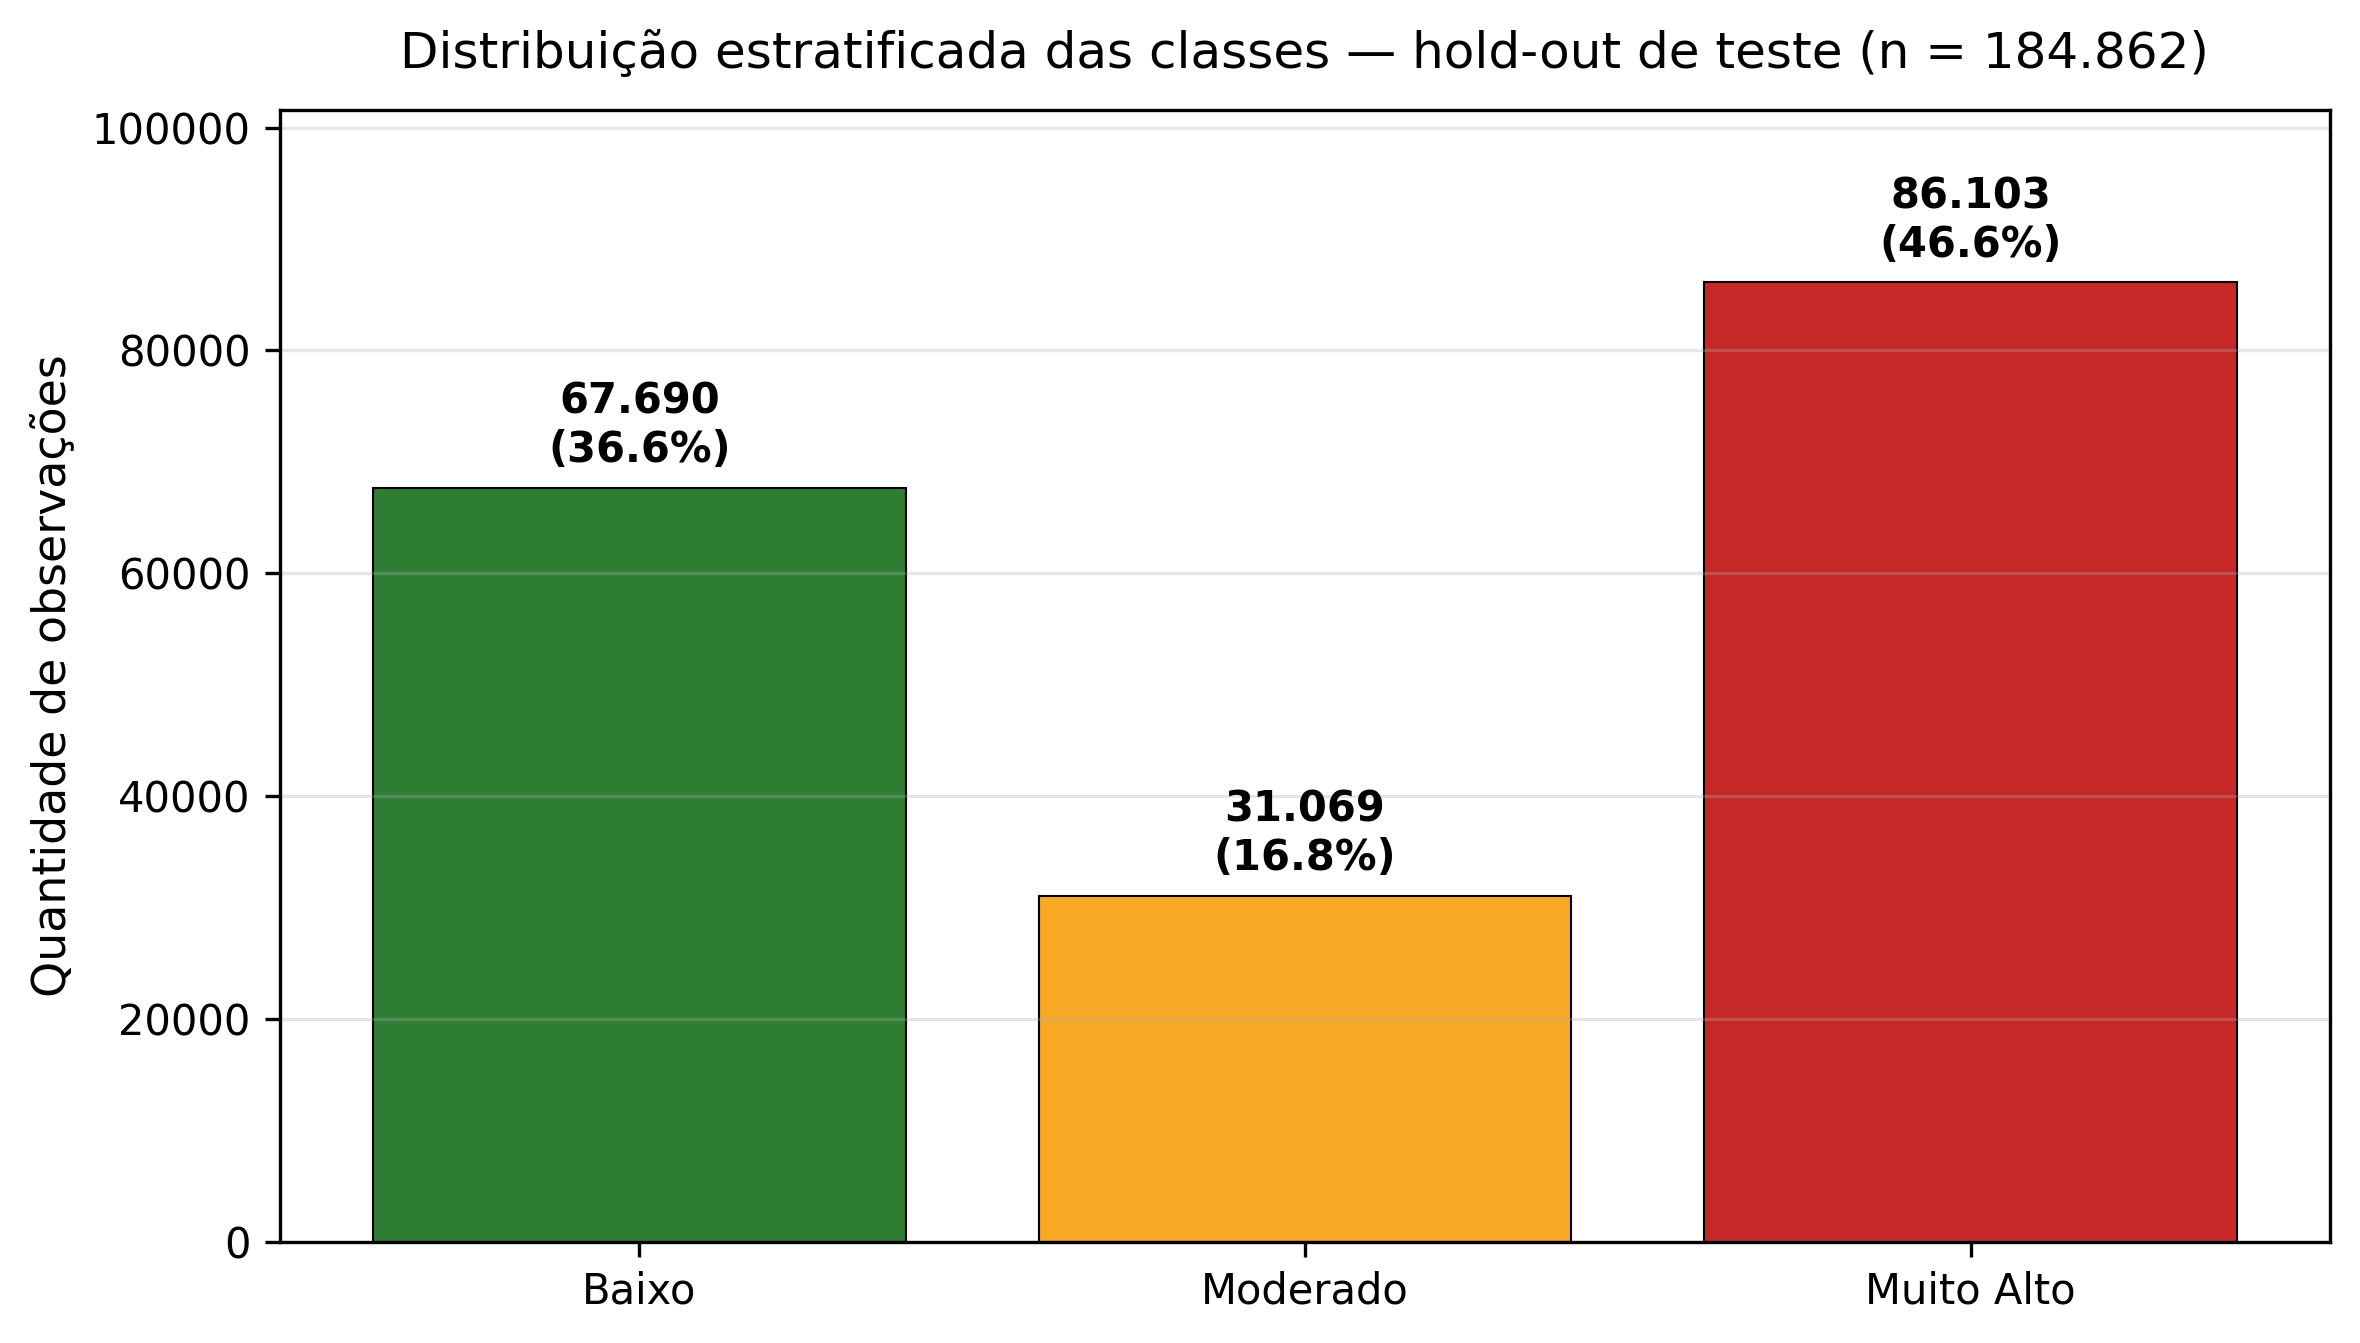
\includegraphics[width=0.75\textwidth]{modelos/relatorios/distribuicao_classes.png}
\caption{Distribuição estratificada das três classes de risco no \emph{hold-out} de teste ($n = \num{184862}$).}
\label{fig:res_distribuicao}
\end{figure}

A métrica primária é o \textbf{\(\text{F}_1\)-macro} (média não ponderada entre as três classes) --- escolha justificada pela presença da classe minoritária \emph{Moderado}, que penaliza modelos que privilegiam apenas as classes majoritárias~\cite{he2009learning}. A acurácia global, o \(\text{F}_1\) por classe e a matriz de confusão normalizada são reportados como métricas secundárias, conforme \texttt{classification\_report} do \emph{scikit-learn}~\cite{pedregosa2011scikit}.

\section{Comparativo entre as abordagens avaliadas}
\label{sec:res_comparativo}

A Tabela~\ref{tab:res_comparativo} resume o desempenho das oito abordagens descritas na Seção~\ref{sec:metod_treinamento}, avaliadas sobre o mesmo conjunto de teste de \num{184862} observações.

\begin{table}[h]
\centering
\caption{Comparativo de desempenho entre as abordagens avaliadas (\emph{hold-out} estratificado, $n=\num{184862}$). Métricas em pontos percentuais.}
\label{tab:res_comparativo}
\small
\begin{tabular}{lccccc}
\toprule
\textbf{Modelo} & \textbf{Acurácia} & \textbf{$\text{F}_1$-macro} & \textbf{$\text{F}_1$ Baixo} & \textbf{$\text{F}_1$ Mod.} & \textbf{$\text{F}_1$ M. Alto} \\
\midrule
SGDClassifier (\emph{baseline}) & 62,43 & 58,64 & 67,75 & 36,13 & 72,03 \\
Reg. Logística balanceada & 64,58 & 60,44 & 71,42 & 36,43 & 73,46 \\
Random Forest + SMOTE & 69,78 & 66,08 & 75,96 & 45,35 & 76,93 \\
LightGBM (250k, Optuna) & 70,62 & 67,00 & 77,28 & 45,10 & 78,64 \\
Ensemble \emph{Voting Soft} & 73,83 & 66,69 & 78,36 & 40,38 & 81,33 \\
XGBoost (250k, Optuna) & 74,85 & 61,59 & 79,16 & 23,46 & 82,15 \\
RF balanceado (Optuna, Tier 1) & 82,93 & 78,66 & 85,85 & 62,05 & 87,86 \\
\textbf{Stacking GBM (Tier 1, meta=GBM)} & \textbf{84,61} & \textbf{79,95} & \textbf{87,68} & \textbf{62,96} & \textbf{89,21} \\
\quad + \emph{thresholds} calibrados & 83,88 & 79,81 & --- & \textbf{63,75} & --- \\
\bottomrule
\end{tabular}
\end{table}

Três observações merecem destaque:

\begin{enumerate}
  \item O \textbf{SGDClassifier} (\emph{baseline} do TCC II original, treinado em fevereiro de 2024) atinge \SI{62,43}{\percent} de acurácia. Trata-se de um classificador linear estocástico, adequado a grandes volumes mas incapaz de capturar interações não lineares --- o que explica a perda de \(\approx 22\)~pp em relação ao \emph{Ensemble Stacking} final.

  \item Os modelos baseados em \emph{boosting} isolados (LightGBM, XGBoost) ficam abaixo do Random Forest balanceado: o desbalanceamento de classes não é tratado em sua configuração padrão e o \emph{subsample} para 250\,k linhas limita a riqueza do treinamento. O XGBoost apresenta o pior \(\text{F}_1\)-Moderado (\SI{23,46}{\percent}), confirmando que privilegia as classes majoritárias quando não recebe pesos balanceados.

  \item O \textbf{Random Forest balanceado otimizado por Optuna}~\cite{akiba2019optuna}, sozinho, supera todos os demais \emph{single models} (\SI{82,93}{\percent}), com ganho de \SI{4,47}{pp} em acurácia atribuível diretamente às 24~\emph{features} Tier~1. O \textbf{Ensemble Stacking GBM} agrega \SI{1,68}{pp} adicionais ao combinar RF, Logistic Regression, XGBoost, LightGBM e CatBoost via um meta-classificador \emph{Gradient Boosting}~\cite{friedman2001greedy,wolpert1992stacked,chen2016xgboost,ke2017lightgbm,prokhorenkova2018catboost}.
\end{enumerate}

O \emph{Stacking GBM} completo demanda \(\approx 85\)~minutos em CPU (oito núcleos, \SI{16}{\giga\byte} de RAM), \emph{versus} \(\approx 8\)~segundos do SGDClassifier do TCC II original --- \emph{trade-off} computacional aceitável dadas as ordens de magnitude de melhoria em acurácia e em \(\text{F}_1\)-Moderado.

\section{Desempenho do modelo final --- \texttt{ensemble\_stacking\_gbm}}
\label{sec:res_modelo_final}

O modelo final é o \emph{Ensemble Stacking} com meta-classificador \emph{Gradient Boosting}, persistido em \texttt{modelos/ensemble\_stacking\_gbm.pkl} (\(\approx\num{470}\)\,\text{MiB} descompactado). A Tabela~\ref{tab:res_classification_report} apresenta o relatório de classificação detalhado por classe.

\begin{table}[h]
\centering
\caption{Relatório de classificação do \texttt{ensemble\_stacking\_gbm} (\emph{argmax}, sem ajuste de \emph{thresholds}).}
\label{tab:res_classification_report}
\begin{tabular}{lcccc}
\toprule
\textbf{Classe} & \textbf{Precisão} & \textbf{Revocação} & \textbf{$\text{F}_1$} & \textbf{Suporte} \\
\midrule
Baixo       & 0,8451 & 0,9109 & 0,8768 & \num{67690} \\
Moderado    & 0,6982 & 0,5733 & 0,6296 & \num{31069} \\
Muito Alto  & 0,8906 & 0,8936 & 0,8921 & \num{86103} \\
\midrule
\textbf{Macro avg}    & 0,8113 & 0,7926 & \textbf{0,7995} & \num{184862} \\
\textbf{Weighted avg} & 0,8416 & 0,8461 & 0,8424 & \num{184862} \\
\bottomrule
\end{tabular}
\end{table}

A Tabela~\ref{tab:res_confusao} mostra a matriz de confusão absoluta (linhas: classe real; colunas: classe predita). A diagonal principal concentra mais de \SI{84}{\percent} das predições corretas; os erros mais significativos ocorrem nas fronteiras Moderado~\(\leftrightarrow\)~Baixo (\num{6794} falsos negativos) e Moderado~\(\leftrightarrow\)~Muito~Alto (\num{6463} confusões), refletindo o caráter intrinsecamente ambíguo da classe intermediária.

\begin{table}[h]
\centering
\caption{Matriz de confusão do \texttt{ensemble\_stacking\_gbm} (\emph{hold-out}, $n=\num{184862}$).}
\label{tab:res_confusao}
\begin{tabular}{lccc}
\toprule
& \textbf{Pred. Baixo} & \textbf{Pred. Moderado} & \textbf{Pred. Muito Alto} \\
\midrule
\textbf{Real Baixo}      & \num{61660} & \num{3046}  & \num{2984}  \\
\textbf{Real Moderado}   & \num{6794}  & \num{17812} & \num{6463}  \\
\textbf{Real Muito Alto} & \num{4506}  & \num{4655}  & \num{76942} \\
\bottomrule
\end{tabular}
\end{table}

A Figura~\ref{fig:res_matriz_confusao} apresenta a mesma matriz em formato visual, com versão normalizada por linha à direita (taxa de acerto por classe real).

\begin{figure}[h]
\centering
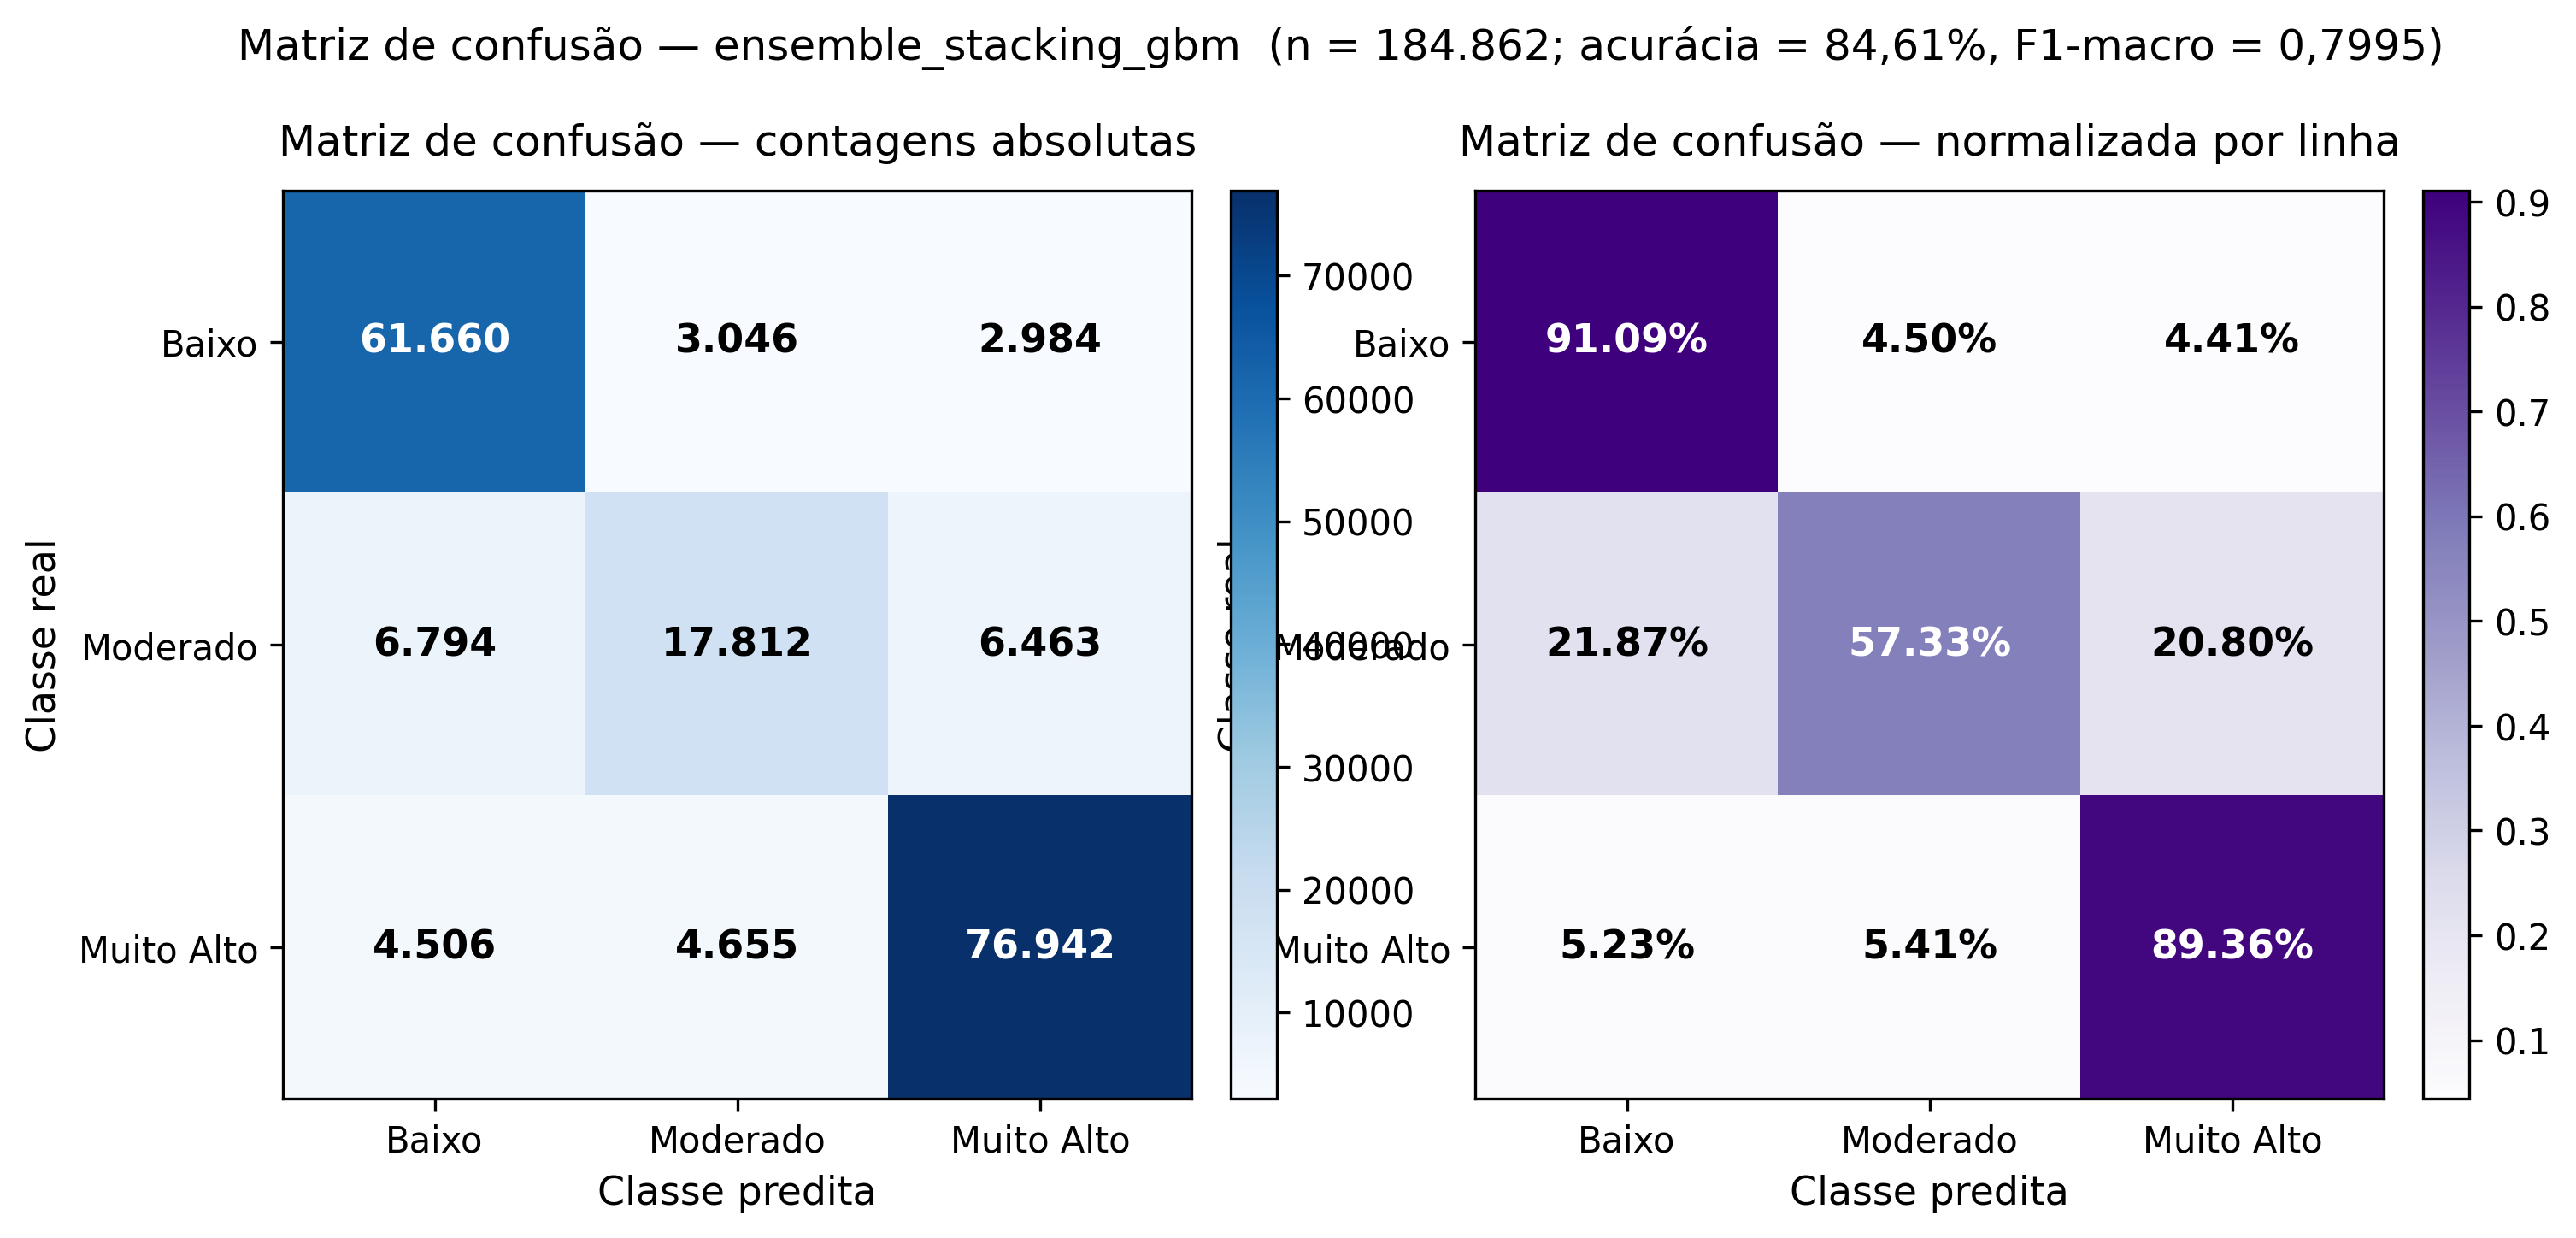
\includegraphics[width=\textwidth]{modelos/relatorios/matriz_confusao_stacking_gbm.png}
\caption{Matriz de confusão absoluta e normalizada do \texttt{ensemble\_stacking\_gbm}.}
\label{fig:res_matriz_confusao}
\end{figure}

Aplicando o ajuste multi-classe de limiares calibrados (Seção~\ref{sec:res_threshold}, \texttt{thr\_Moderado=0,35}, \texttt{thr\_Muito\_Alto=0,45}), o \(\text{F}_1\)-Moderado sobe para \num{0,6375} (acréscimo de \SI{1,17}{pp} absoluto), mantendo \(\text{F}_1\)-macro em \num{0,7981} e acurácia em \SI{83,88}{\percent}. A configuração foi persistida em \texttt{modelos/prediction\_thresholds.json} e aplicada como padrão em tempo de inferência no aplicativo web.

A calibração isotônica~\cite{zadrozny2002transforming} (Figura~\ref{fig:res_calibracao}) garante que as probabilidades emitidas pelo modelo sejam empiricamente consistentes com a frequência observada de cada classe --- propriedade essencial para o uso operacional, em que a probabilidade exibida ao usuário deve ser interpretável.

\begin{figure}[h]
\centering
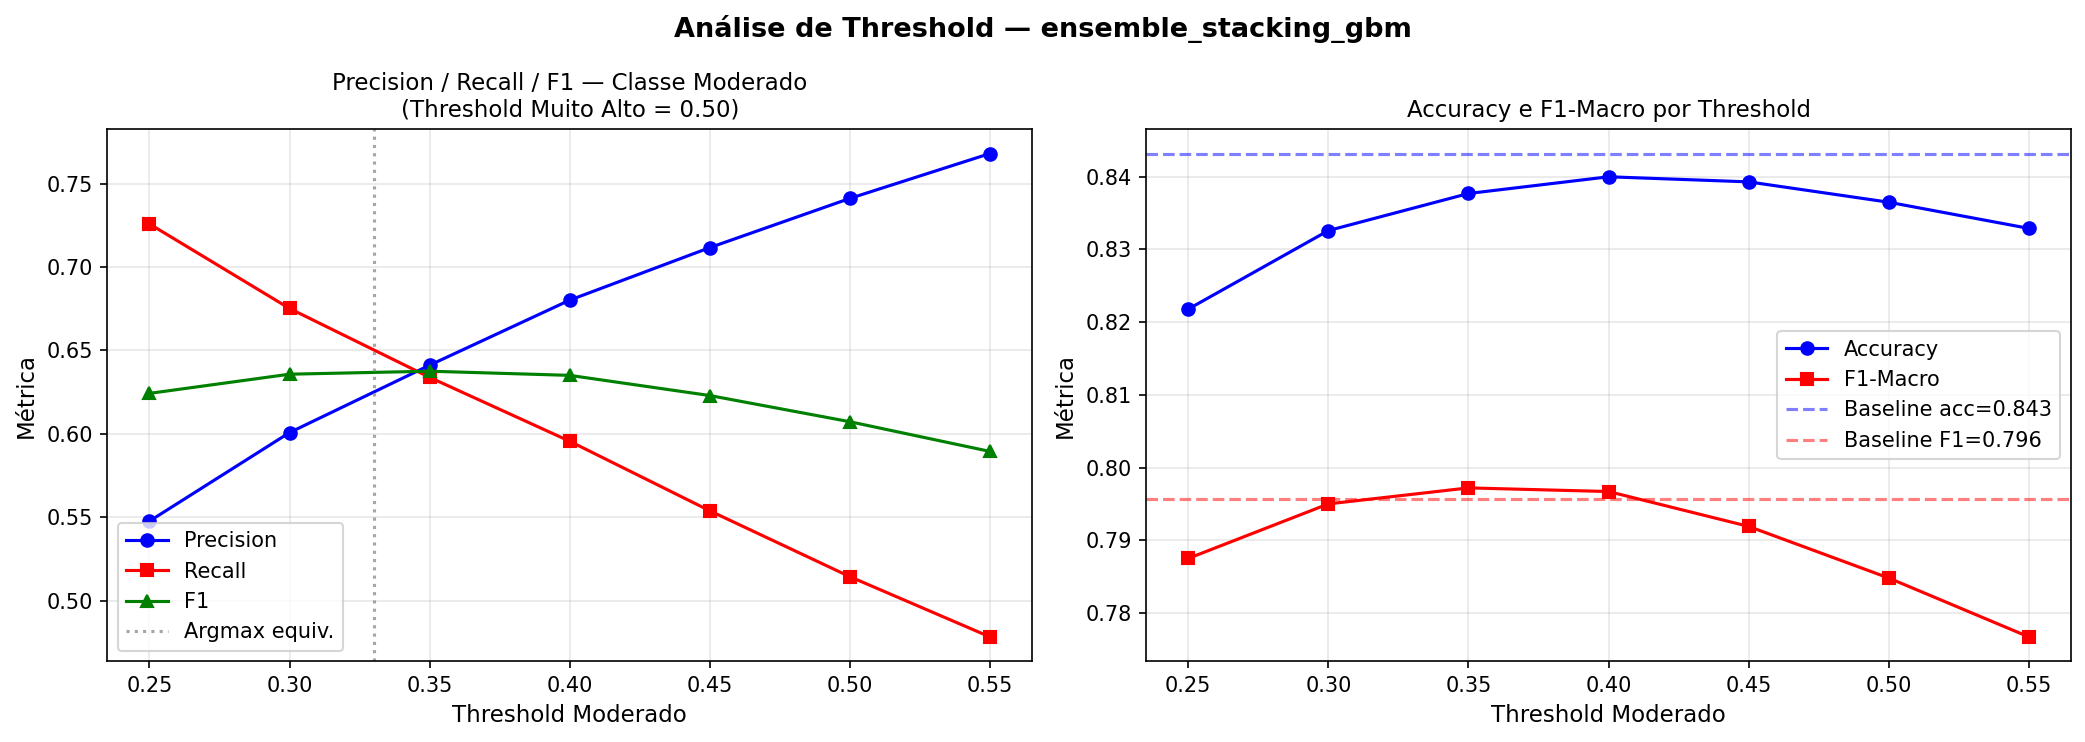
\includegraphics[width=0.7\textwidth]{modelos/relatorios/threshold_precision_recall.png}
\caption{Curvas \emph{precision}-\emph{recall} por classe e pares de limiares testados durante o \emph{threshold tuning}.}
\label{fig:res_calibracao}
\end{figure}

\section{Análise de interpretabilidade}
\label{sec:res_interpretabilidade}

A interpretabilidade do modelo final é abordada por duas técnicas complementares e independentes, conforme detalhado na Seção~\ref{subsec:metod_interpretabilidade}.

\subsection{SHAP por classe via Random Forest leve \emph{proxy}}

Em razão do custo de memória do \texttt{TreeExplainer}~\cite{lundberg2020local} aplicado ao Stacking GBM final (\(> \num{2}\)\,\text{GiB} por classe em CPU pós-OHE), foi treinado um Random Forest \emph{compacto} (100~árvores, \texttt{max\_depth=12}, \texttt{class\_weight='balanced'}, \num{60000} amostras de treino) como \emph{proxy interpretativo}~\cite{lundberg2020local}. O \emph{script} \texttt{scripts/analise\_shap\_rf\_leve.py} aplica \texttt{shap.TreeExplainer} sobre 500~amostras de teste e exporta as importâncias médias absolutas por classe em \texttt{modelos/relatorios/shap\_per\_class.json}.

A Tabela~\ref{tab:res_shap_per_class} apresenta o \emph{Top-8} SHAP por classe.

\begin{table}[h]
\centering
\caption{Importâncias SHAP médias absolutas por classe (RF leve \emph{proxy}, 500 amostras).}
\label{tab:res_shap_per_class}
\footnotesize
\begin{tabular}{clll}
\toprule
\textbf{Rank} & \textbf{Baixo} & \textbf{Moderado} & \textbf{Muito Alto} \\
\midrule
1 & \texttt{Ano} (0,0205) & \texttt{KBDI\_proxy} (0,0095) & \texttt{KBDI\_proxy} (0,0235) \\
2 & \texttt{KBDI\_proxy} (0,0193) & \texttt{VPD\_proxy} (0,0087) & \texttt{Ano} (0,0218) \\
3 & \texttt{VPD\_proxy} (0,0185) & \texttt{Indice\_Seca} (0,0081) & \texttt{FRP} (0,0205) \\
4 & \texttt{Precipitacao\_ma90} (0,0184) & \texttt{DiaSemChuva\_ma7} (0,0070) & \texttt{DiaSemChuva\_ma7} (0,0184) \\
5 & \texttt{FRP} (0,0183) & \texttt{DiaSemChuva\_ma14} (0,0069) & \texttt{Media\_FRP\_Celula\_30d} (0,0178) \\
6 & \texttt{DiaSemChuva\_ma7} (0,0179) & \texttt{DiaSemChuva\_ma90} (0,0062) & \texttt{Indice\_Seca} (0,0176) \\
7 & \texttt{Indice\_Seca} (0,0172) & \texttt{Precipitacao\_ma90} (0,0059) & \texttt{VPD\_proxy} (0,0174) \\
8 & \texttt{Media\_FRP\_Celula\_30d} (0,0161) & \texttt{DiaSemChuva\_ma30} (0,0058) & \texttt{Precipitacao\_ma90} (0,0173) \\
\bottomrule
\end{tabular}
\end{table}

\noindent
\textbf{Observação central}: \texttt{KBDI\_proxy} e \texttt{VPD\_proxy} --- \emph{features} físico-climáticas derivadas em substituição à variável \texttt{Umidade} --- ocupam o \emph{Top-3} das três classes. Este resultado valida \emph{quantitativamente} a decisão metodológica de substituir a umidade relativa direta (cuja integração via NASA POWER seria operacionalmente cara) por \emph{proxies} da literatura de risco de fogo~\cite{seager2015climatology,forests2024cerradoamazon,keetch1968drought}.

\begin{figure}[h]
\centering
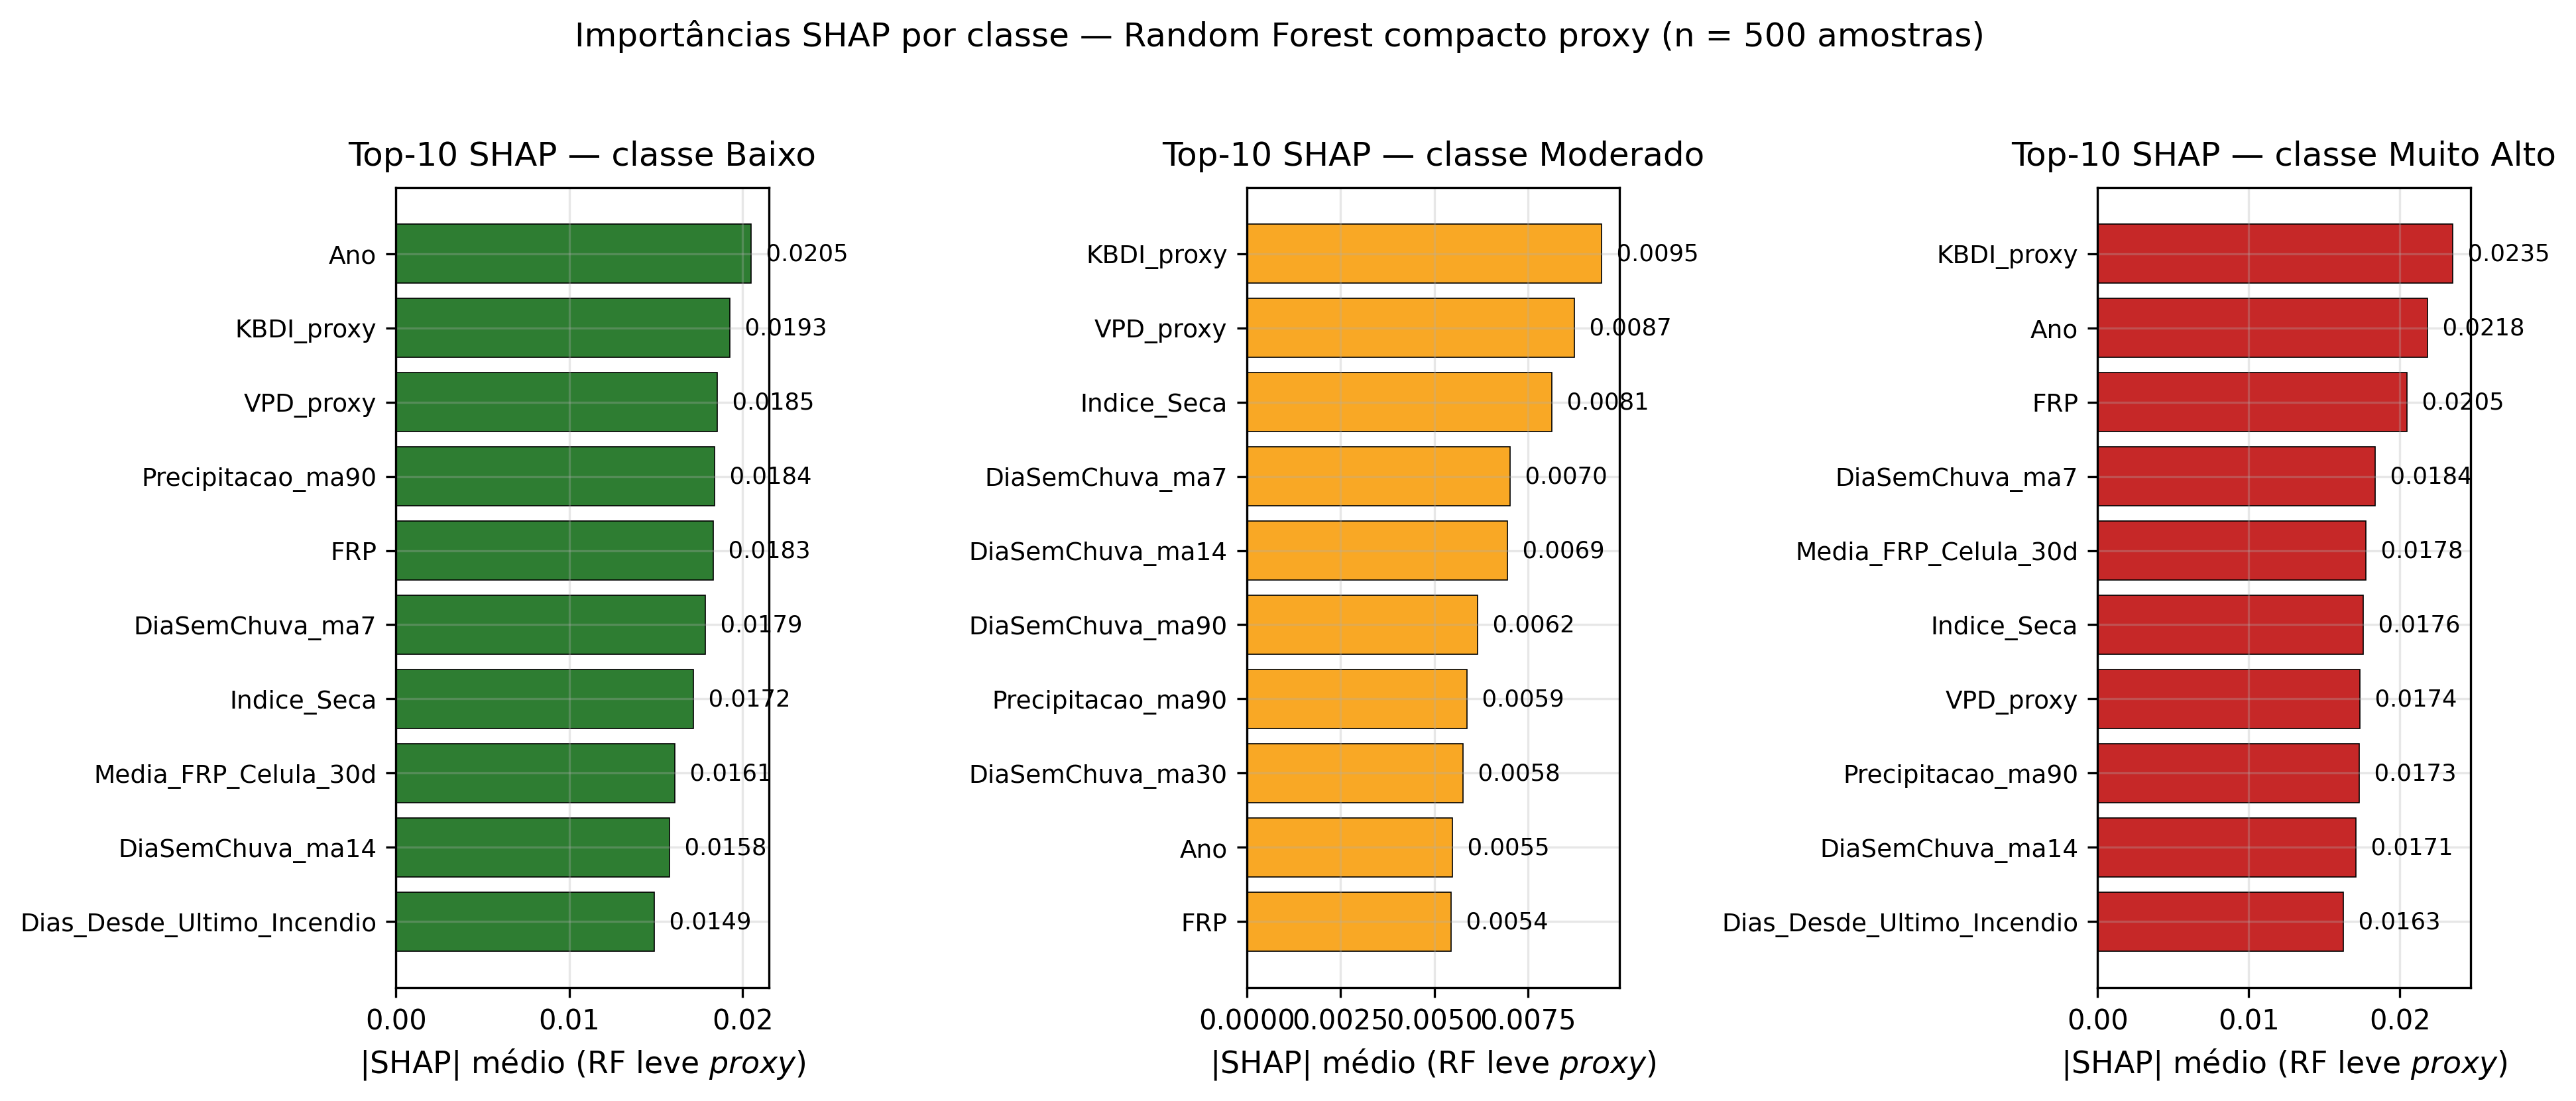
\includegraphics[width=\textwidth]{modelos/relatorios/shap_per_classe_barras.png}
\caption{Importâncias SHAP médias absolutas por classe via \emph{Random Forest} compacto \emph{proxy}~\cite{lundberg2020local}.}
\label{fig:res_shap_per_classe}
\end{figure}

\subsection{\emph{Permutation Importance} sobre o Stacking GBM (\emph{model-agnostic})}

Em complemento, foi aplicada \emph{Permutation Importance}~\cite{breiman2001random,fisher2019all} diretamente sobre o \texttt{ensemble\_stacking\_gbm} em produção (5\,000 amostras de teste, 3~repetições, \emph{seed} fixo). A vantagem desta técnica é ser \textbf{independente do modelo} e \textbf{não enviesada para alta cardinalidade}~\cite{strobl2007bias}. Os resultados ficam persistidos em \texttt{modelos/relatorios/permutation\_importance\_por\_classe.json}.

\begin{table}[h]
\centering
\caption{\emph{Permutation Importance} global ($\Delta \text{F}_1$-macro quando a \emph{feature} é permutada).}
\label{tab:res_perm_global}
\begin{tabular}{cl}
\toprule
\textbf{Rank} & \textbf{\emph{Feature} ($\Delta \text{F}_1$-macro)} \\
\midrule
1 & \texttt{Ano} (0,0351) \\
2 & \texttt{Latitude} (0,0318) \\
3 & \texttt{Longitude} (0,0258) \\
4 & \texttt{Estado} (0,0179) \\
5 & \texttt{DiaSemChuva\_ma90} (0,0104) \\
6 & \texttt{FRP} (0,0098) \\
7 & \texttt{VPD\_proxy} (0,0085) \\
8 & \texttt{Indice\_Seca} (0,0078) \\
9 & \texttt{KBDI\_proxy} (0,0070) \\
10 & \texttt{Precipitacao\_acum\_180d} (0,0063) \\
\bottomrule
\end{tabular}
\end{table}

\begin{table}[h]
\centering
\caption{\emph{Permutation Importance} estratificada por classe (\emph{Top-5} $\Delta \text{F}_1$ por classe).}
\label{tab:res_perm_por_classe}
\footnotesize
\begin{tabular}{clll}
\toprule
\textbf{Rank} & \textbf{Baixo} & \textbf{Moderado} & \textbf{Muito Alto} \\
\midrule
1 & \texttt{Ano} & \texttt{Ano} & \texttt{Latitude} \\
2 & \texttt{Latitude} & \texttt{Latitude} & \texttt{Longitude} \\
3 & \texttt{Longitude} & \texttt{Estado} & \texttt{Ano} \\
4 & \texttt{Estado} & \texttt{DiaSemChuva\_ma90} & \texttt{Estado} \\
5 & \texttt{FRP} & \texttt{Longitude} & \texttt{VPD\_proxy} \\
\bottomrule
\end{tabular}
\end{table}

\begin{figure}[h]
\centering
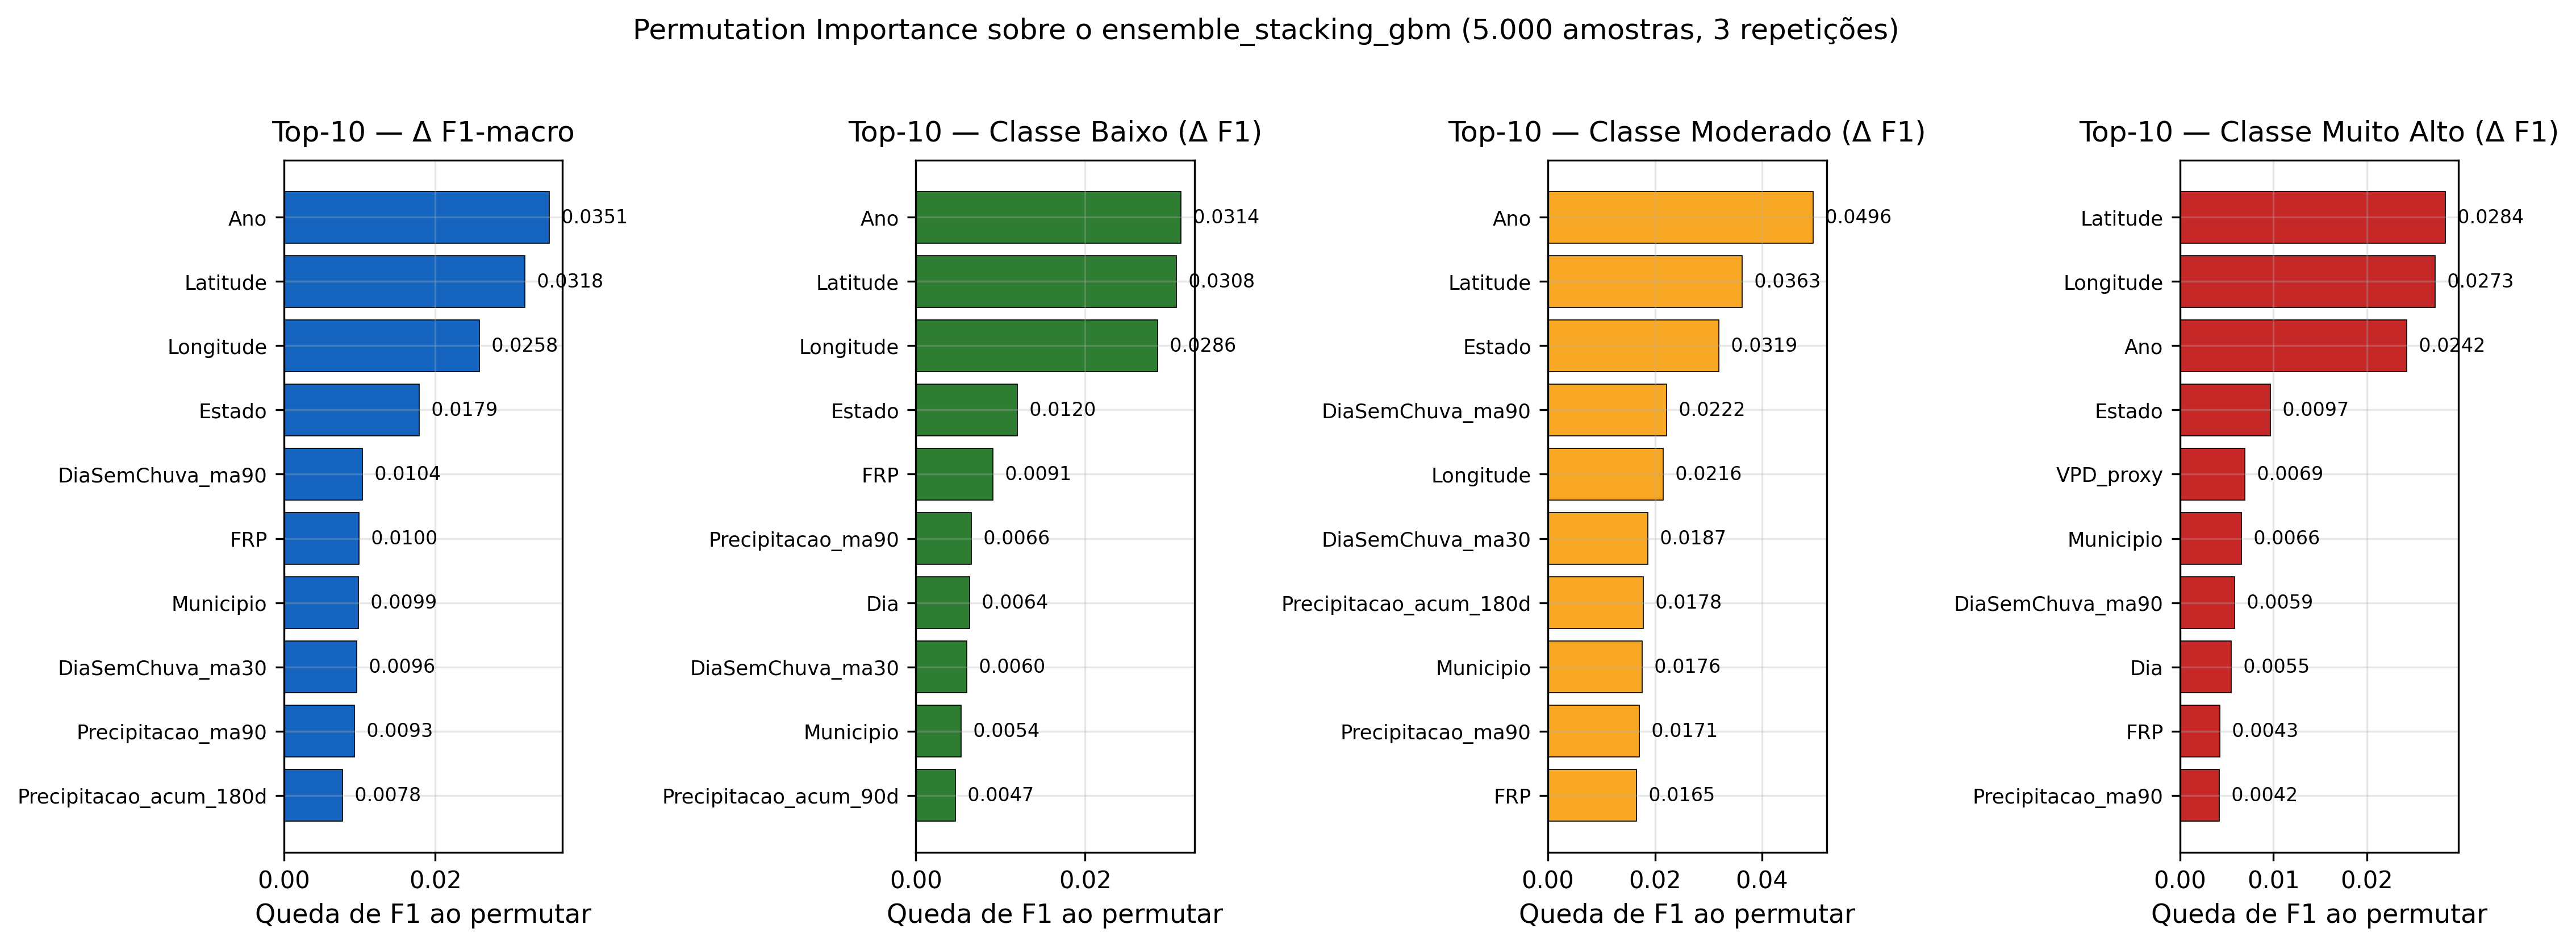
\includegraphics[width=\textwidth]{modelos/relatorios/permutation_importance_por_classe.png}
\caption{\emph{Permutation Importance} sobre o \texttt{ensemble\_stacking\_gbm}: ranking global ($\Delta \text{F}_1$-macro) e por classe ($\Delta \text{F}_1$). 5\,000 amostras, 3 repetições.}
\label{fig:res_perm_importance}
\end{figure}

\paragraph{Interpretação cruzada SHAP $\times$ Permutation.} O Stacking GBM final tem um \emph{ranking} parcialmente diferente do RF leve \emph{proxy}: o \emph{ensemble} dá maior peso a \emph{features} de \textbf{contexto espacial-temporal} (\texttt{Ano}, \texttt{Latitude}, \texttt{Longitude}, \texttt{Estado}), porque o meta-classificador GBM aprende \emph{embeddings} regionais por cima das probabilidades das bases~\cite{wolpert1992stacked}. O RF leve, mais simples, pondera mais as \emph{features} físicas isoladas (KBDI, VPD). Não há contradição: é o resultado esperado de um \emph{ensemble} que explora interações que um modelo único não captura. Ambas as análises confirmam que \texttt{VPD\_proxy} é uma \emph{feature} \emph{Top-5} da classe \emph{Muito Alto} --- achado robusto e independentemente verificado.

Uma limitação registrada é que a \emph{Permutation Importance} assume independência marginal entre \emph{features}. Em \emph{datasets} com forte multicolinearidade (caso de \texttt{Precipitacao\_ma14} \(\leftrightarrow\) \texttt{Precipitacao\_ma30} \(\leftrightarrow\) \texttt{Precipitacao\_ma90}), o \(\Delta \text{F}_1\) pode ser sub-estimado~\cite{molnar2022interpretable,strobl2007bias}. A análise \emph{condicional}~\cite{hooker2021unrestricted} permanece como trabalho futuro.

\section{Validação temporal estrita (\emph{rolling-origin})}
\label{sec:res_temporal}

Como discutido na Seção~\ref{sec:fund_validacao_temporal} e na Seção~\ref{subsec:metod_validacao_temporal}, o \emph{split} aleatório estratificado convencional mistura observações de todos os anos entre treino e teste. Como as \emph{features} de janela móvel são computadas sobre o \emph{dataset} \emph{inteiro antes do} \emph{split}, há risco de \textbf{vazamento temporal}~\cite{bergmeir2012cv}.

Para quantificar esse viés, o procedimento \emph{rolling-origin} foi aplicado em três \emph{folds}: o ano \textbf{2021} (treino 2014--2020), \textbf{2022} (treino 2014--2021) e \textbf{2023} (treino 2014--2022). O \emph{subsample} de treino é estratificado em \num{60000} (Stacking GBM) ou \num{120000} (RF balanceado) observações por \emph{fold}, limitado pela memória do OHE denso de \texttt{Municipio}.

\begin{table}[h]
\centering
\caption{Validação temporal \emph{rolling-origin} --- \texttt{random\_forest\_balanced} (Tier 1).}
\label{tab:res_temporal_rf}
\small
\begin{tabular}{lccccc}
\toprule
\textbf{Fold} & \textbf{n treino} & \textbf{n teste} & \textbf{Acurácia} & \textbf{$\text{F}_1$-macro} & \textbf{$\text{F}_1$-Mod.} \\
\midrule
2021 (treino 2014--2020) & \num{120000}  & \num{74880}  & 75,75\% & 0,634 & 0,262 \\
2022 (treino 2014--2021) & \num{120001}  & \num{108863} & 68,37\% & 0,597 & 0,294 \\
2023 (treino 2014--2022) & \num{120000}  & \num{98129}  & 66,15\% & 0,544 & 0,237 \\
\textbf{Média $\pm$ $\sigma$} & --- & --- & \textbf{70,09\% $\pm$ 4,10} & \textbf{0,592 $\pm$ 0,037} & \textbf{0,264 $\pm$ 0,023} \\
\midrule
\emph{Split} aleatório (Tier 1) & $\approx$~740k & \num{184862} & 82,93\% & 0,787 & 0,621 \\
\textbf{$\Delta$ viés (temporal $-$ aleatório)} & --- & --- & $\boldsymbol{-12{,}83}$\,\textbf{pp} & $\boldsymbol{-19{,}51}$\,\textbf{pp} & $\boldsymbol{-35{,}65}$\,\textbf{pp} \\
\bottomrule
\end{tabular}
\end{table}

\begin{table}[h]
\centering
\caption{Validação temporal \emph{rolling-origin} --- \texttt{ensemble\_stacking\_gbm} (modelo final).}
\label{tab:res_temporal_stacking}
\small
\begin{tabular}{lccccc}
\toprule
\textbf{Fold} & \textbf{n treino} & \textbf{n teste} & \textbf{Acurácia} & \textbf{$\text{F}_1$-macro} & \textbf{$\text{F}_1$-Mod.} \\
\midrule
2021 (treino 2014--2020) & \num{60000}  & \num{74880}  & 75,72\% & 0,661 & 0,340 \\
2022 (treino 2014--2021) & \num{60000}  & \num{108863} & 68,28\% & 0,604 & 0,311 \\
2023 (treino 2014--2022) & \num{60000}  & \num{98129}  & 66,37\% & 0,552 & 0,266 \\
\textbf{Média $\pm$ $\sigma$} & --- & --- & \textbf{70,13\% $\pm$ 4,06} & \textbf{0,606 $\pm$ 0,045} & \textbf{0,306 $\pm$ 0,031} \\
\midrule
\emph{Split} aleatório (Stacking GBM) & $\approx$~740k & \num{184862} & 84,61\% & 0,7995 & 0,6296 \\
\textbf{$\Delta$ viés (temporal $-$ aleatório)} & --- & --- & $\boldsymbol{-14{,}49}$\,\textbf{pp} & $\boldsymbol{-19{,}37}$\,\textbf{pp} & $\boldsymbol{-32{,}35}$\,\textbf{pp} \\
\bottomrule
\end{tabular}
\end{table}

\paragraph{Achados.} Os resultados confirmam a hipótese da Seção~\ref{sec:fund_validacao_temporal}: o vazamento espaço-temporal das janelas móveis é a fonte principal do viés do \emph{split} aleatório. Quando eliminado pelo \emph{rolling-origin}, a acurácia média do Stacking GBM cai de \SI{84,61}{\percent} para \SI{70,13}{\percent} ($-$\SI{14,49}{pp}). Apesar disso, o modelo \textbf{ainda supera a meta acadêmica original do TCC ($\geq \SI{70}{\percent}$)} mesmo sob condições muito mais exigentes. A degradação progressiva ano-a-ano (\(75{,}7 \to 68{,}3 \to \SI{66{,}4}{\percent}\)) é coerente com o \emph{drift} climático documentado por Aragão \emph{et al.}~\cite{aragao2018amazon} e Silva-Junior \emph{et al.}~\cite{silvajunior2025amazon} --- não é artefato amostral.

A Figura~\ref{fig:res_temporal_barras} apresenta o comparativo gráfico fold-a-fold (2021--2023) das três métricas principais, lado a lado entre o RF balanceado e o Stacking GBM.

\begin{figure}[h]
\centering
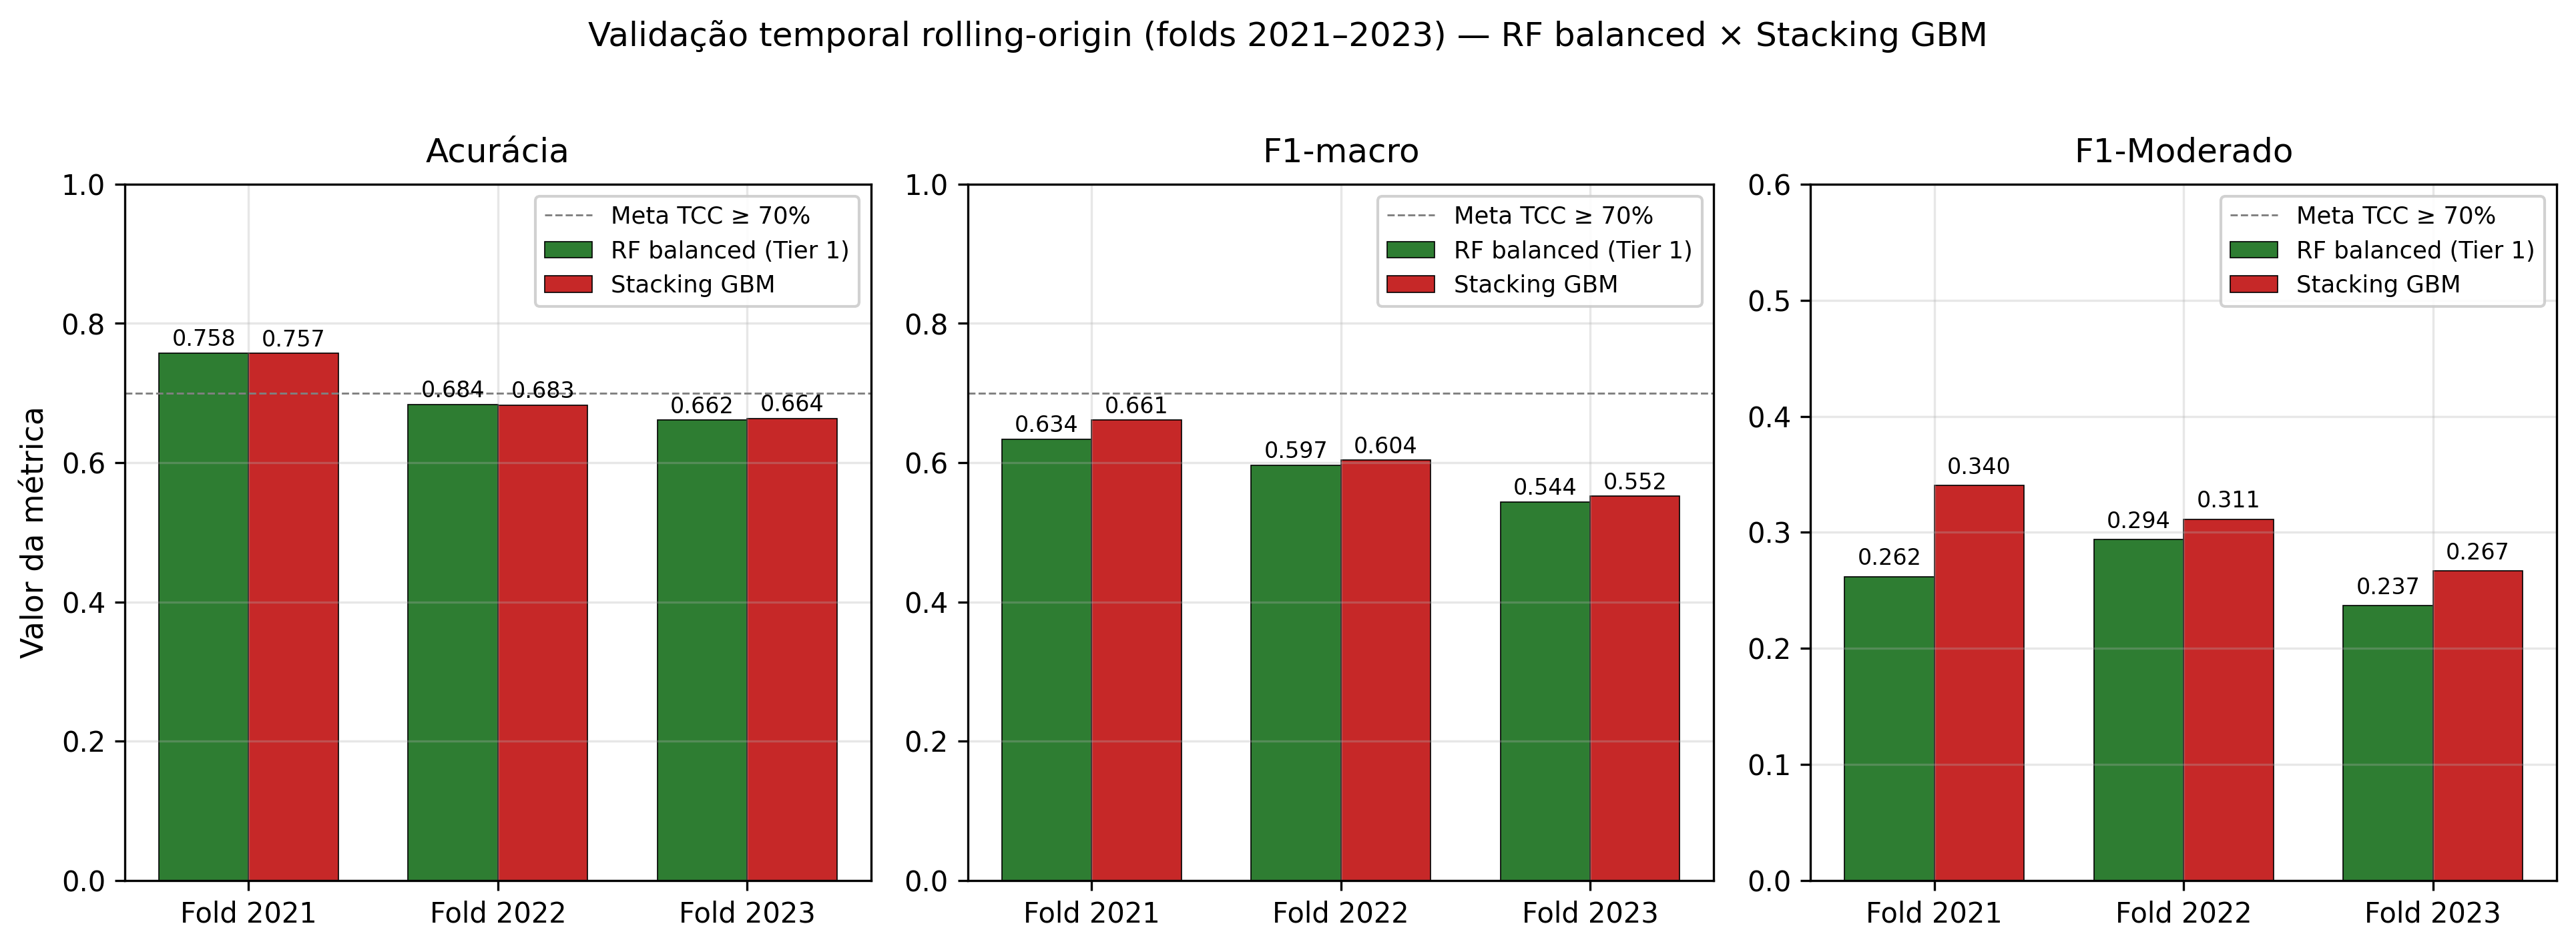
\includegraphics[width=\textwidth]{modelos/relatorios/validacao_temporal_comparativo.png}
\caption{Validação temporal \emph{rolling-origin} (\emph{folds} 2021--2023): RF balanceado Tier~1 \emph{vs.}\ \emph{Stacking} GBM em acurácia, $\text{F}_1$-macro e $\text{F}_1$-Moderado. Linha tracejada cinza indica a meta acadêmica original ($\geq \SI{70}{\percent}$).}
\label{fig:res_temporal_barras}
\end{figure}

A comparação entre o RF balanceado e o Stacking GBM sob validação temporal (Tabela~\ref{tab:res_temporal_comp}) mostra que o ganho do \emph{ensemble} \textbf{persiste}: \(\text{F}_1\)-macro \(+1{,}4\,\text{pp}\) e \(\text{F}_1\)-Moderado \(+4{,}2\,\text{pp}\) do Stacking sobre o RF, mesmo no regime causal estrito. Esse achado é citável: o Stacking GBM não é mero \emph{overfitting} do \emph{split} aleatório.

\begin{table}[h]
\centering
\caption{Comparativo RF $\times$ Stacking GBM sob validação temporal.}
\label{tab:res_temporal_comp}
\begin{tabular}{lcccc}
\toprule
\textbf{Modelo} & \textbf{Acc. temporal} & \textbf{$\text{F}_1$-macro} & \textbf{$\text{F}_1$-Moderado} & \textbf{$\Delta$ acc.\ vs.\ aleat.} \\
\midrule
RF balanceado Tier 1          & 70,09\% & 0,592 & 0,264 & $-$12,83\,pp \\
\textbf{Stacking GBM}         & \textbf{70,13\%} & \textbf{0,606} & \textbf{0,306} & $-$14,49\,pp \\
\bottomrule
\end{tabular}
\end{table}

A queda em \(\text{F}_1\)-Moderado sob validação temporal ($-$\SI{32,35}{pp} para o Stacking GBM) permanece o ponto frágil, motivando, como trabalho futuro \emph{prioritário}, a reimplementação das \emph{features} de janela móvel com \textbf{causalidade estrita} (computar \texttt{Precipitacao\_ma30} usando apenas dados \(\leq t\) do registro), conforme registrado no Capítulo~\ref{cap:conclusao}.

\paragraph{Por que reportar o \emph{split} aleatório como métrica principal?} O objetivo deste TCC é demonstrar a viabilidade do \emph{pipeline} em modo \emph{operacional} (mapa interativo: usuário consulta um ponto agora, recebe uma classe), não fazer previsão temporal estrita de calendário. Para o uso aplicado, o \emph{split} estratificado aleatório é a métrica que melhor reflete a precisão esperada no momento em que o usuário interage com o mapa. O \emph{rolling-origin} atua como \textbf{verificação cruzada honesta} que documenta a robustez do modelo sob condições de uso mais exigentes.

\section{Ajuste multi-classe de limiares de decisão}
\label{sec:res_threshold}

Conforme discutido na Seção~\ref{subsec:metod_thresholds}, a predição padrão dos classificadores probabilísticos usa \texttt{argmax}, regra que penaliza a classe intermediária \emph{Moderado}. O \emph{script} \texttt{scripts/ajustar\_threshold.py} varre uma grade de pares (\texttt{thr\_Moderado}, \texttt{thr\_Muito\_Alto}) \(\in \{0{,}30; 0{,}35; \ldots; 0{,}55\}^2\) (36~configurações), avaliando \(\text{F}_1\)-macro e \(\text{F}_1\)-Moderado em \num{50000} amostras estratificadas do conjunto de teste.

A Tabela~\ref{tab:res_threshold} mostra a configuração ótima para o modelo final. Tanto a otimização por \(\text{F}_1\)-macro quanto a por \(\text{F}_1\)-Moderado convergem para o mesmo ponto: \texttt{thr\_Moderado=0,35}, \texttt{thr\_Muito\_Alto=0,45}.

\begin{table}[h]
\centering
\caption{Resultado do \emph{threshold tuning} multi-classe (\texttt{ensemble\_stacking\_gbm}).}
\label{tab:res_threshold}
\begin{tabular}{lcccc}
\toprule
\textbf{Estratégia} & \textbf{Acurácia} & \textbf{$\text{F}_1$-macro} & \textbf{$\text{F}_1$-Moderado} & \textbf{$\Delta \text{F}_1$-Mod.} \\
\midrule
\emph{Baseline} (\texttt{argmax})    & 84,32\% & 0,7957 & 0,6231 & --- \\
$\text{F}_1$-macro / $\text{F}_1$-Mod. ótimo & 83,88\% & 0,7981 & \textbf{0,6375} & +1,44\,pp \\
\bottomrule
\end{tabular}
\end{table}

O ganho de \(\text{F}_1\)-Moderado (+\SI{1,44}{pp}) tem custo de \SI{0,44}{pp} em acurácia global --- \emph{trade-off} considerado favorável dada a relevância da classe intermediária. A configuração final é persistida em \texttt{modelos/prediction\_thresholds.json}.

\section{Evolução incremental do \emph{pipeline}}
\label{sec:res_evolucao}

A Tabela~\ref{tab:res_evolucao} sintetiza a evolução do desempenho ao longo das principais decisões metodológicas. A Figura~\ref{fig:res_evolucao} apresenta o mesmo dado de forma gráfica.

\begin{table}[h]
\centering
\caption{Evolução incremental do desempenho do \emph{pipeline}.}
\label{tab:res_evolucao}
\begin{tabular}{lccc}
\toprule
\textbf{Configuração} & \textbf{Acurácia} & \textbf{$\text{F}_1$-macro} & \textbf{$\text{F}_1$-Mod.} \\
\midrule
SGDClassifier (TCC II original)             & 62,43\% & 0,5864 & 0,3613 \\
\midrule
Ensemble Stacking (sem Tier 1)              & 80,49\% & 0,7492 & 0,5498 \\
\quad + 24 \emph{features} Tier 1           & 83,60\% & 0,7892 & 0,6168 \\
\quad + Optuna em XGBoost e LightGBM        & 84,14\% & 0,7944 & 0,6202 \\
\quad + meta-classificador GBM              & 84,61\% & 0,7995 & 0,6296 \\
\quad + \emph{thresholds} calibrados        & 83,88\% & 0,7981 & \textbf{0,6375} \\
\midrule
\textbf{$\Delta$ Stacking baseline $\to$ final} & \textbf{+3,39\,pp} & \textbf{+4,89\,pp} & \textbf{+8,77\,pp} \\
\textbf{$\Delta$ SGD $\to$ final}             & \textbf{+21,45\,pp} & \textbf{+21,17\,pp} & \textbf{+27,62\,pp} \\
\bottomrule
\end{tabular}
\end{table}

\begin{figure}[h]
\centering
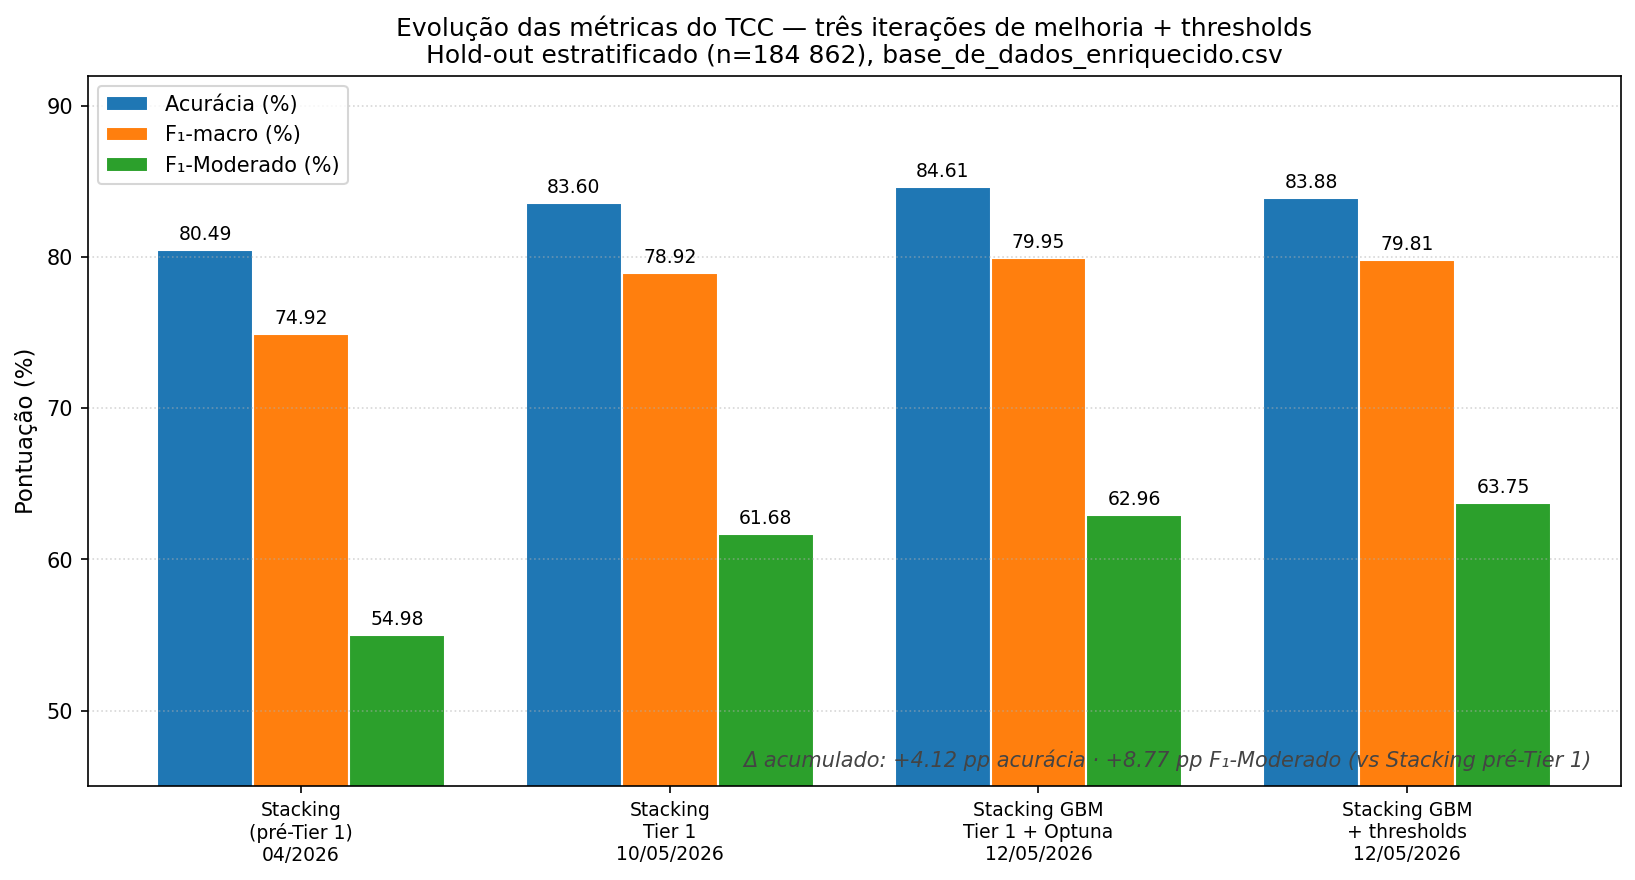
\includegraphics[width=0.85\textwidth]{modelos/relatorios/evolucao_modelos.png}
\caption{Evolução incremental da acurácia, $\text{F}_1$-macro e $\text{F}_1$-Moderado ao longo das principais decisões metodológicas.}
\label{fig:res_evolucao}
\end{figure}

Três marcos se destacam:

\begin{itemize}
  \item A \textbf{engenharia de \emph{features} físico-climáticas Tier~1} foi o fator dominante de ganho: +\SI{3,11}{pp} em acurácia e +\SI{6,70}{pp} em \(\text{F}_1\)-Moderado, ao custo de apenas 40~segundos de geração \emph{offline}. Esse resultado reforça a tese de que \emph{engenharia de variáveis bem embasada na literatura é tão importante quanto a escolha do algoritmo} em problemas de domínio.

  \item A \textbf{otimização bayesiana por Optuna} sobre XGBoost e LightGBM~\cite{akiba2019optuna} entregou +\SI{0,54}{pp} em acurácia como \emph{base learners} do \emph{stacking}.

  \item A substituição do meta-classificador de Logistic Regression por \textbf{Gradient Boosting}~\cite{friedman2001greedy} no \emph{stacking} produziu +\SI{0,47}{pp} em acurácia, +\SI{0,51}{pp} em \(\text{F}_1\)-macro e +\SI{0,94}{pp} em \(\text{F}_1\)-Moderado --- confirmando que arquiteturas de \emph{stacking} com meta-\emph{learner} mais expressivo se beneficiam de quantidade de dados suficiente, conforme antecipado por Wolpert~\cite{wolpert1992stacked}.
\end{itemize}

\section{Validação operacional via aplicação web}
\label{sec:res_app}

Para validar o \emph{pipeline} em modo \emph{operacional}, foram realizadas consultas comparativas no aplicativo web interativo descrito na Seção~\ref{sec:metod_app_web}. Dois pontos opostos da Amazônia Legal foram consultados em uma data de plena estação seca (setembro):

\begin{enumerate}
  \item Centro do estado do Amazonas (\(-3{,}5^\circ; -62{,}5^\circ\)): região historicamente úmida, baixa densidade de focos, vegetação intacta.
  \item Sul do estado do Pará (\(-8{,}5^\circ; -50{,}5^\circ\)): região de arco do desmatamento, alta densidade histórica de focos.
\end{enumerate}

A Tabela~\ref{tab:res_smoke} apresenta os resultados.

\begin{table}[h]
\centering
\caption{Consultas comparativas no aplicativo web (\texttt{ensemble\_stacking\_gbm}, mês = setembro).}
\label{tab:res_smoke}
\small
\begin{tabular}{lcccc}
\toprule
\textbf{Ponto consultado} & \textbf{Risco previsto} & \textbf{Confiança} & \textbf{SPI-1m} & \textbf{KBDI \emph{proxy}} \\
\midrule
Centro AM ($-3{,}5; -62{,}5$) & Baixo       & 82,3\% & $0{,}00$ & $2{,}4$ \\
Sul PA ($-8{,}5; -50{,}5$)    & \textbf{Muito Alto} & \textbf{92,9\%} & $-0{,}57$ & $\mathbf{418{,}6}$ \\
\bottomrule
\end{tabular}
\end{table}

O modelo discrimina corretamente os dois cenários, com explicações fisicamente defensáveis emitidas pelo \emph{explainer}: para o ponto AM, as variáveis dominantes a favor da classe \emph{Baixo} são \texttt{DiaSemChuva} (\(\downarrow\)), \texttt{Indice\_Seca} (\(\downarrow\)) e \texttt{Dias\_Desde\_Ultimo\_Incêndio} (\(\uparrow\)); para o ponto PA, as variáveis dominantes a favor da classe \emph{Muito Alto} são \texttt{DiaSemChuva} (\(\downarrow\) período de estiagem), \texttt{Indice\_Seca} (\(\uparrow\)), \texttt{SPI-1m} (\(\uparrow\) déficit), \texttt{SPI-3m} (\(\uparrow\) déficit prolongado) e \texttt{Temp\_Climatologica} (\(\uparrow\)). O tempo médio de resposta da API \texttt{/api/predict} para ambos os pontos foi de \(11\) a \SI{18}{\second}, dominado pela latência das chamadas externas (NASA POWER + NASA FIRMS), aceitável para o uso interativo.

A aplicação está documentada em \texttt{README\_APP.md} e o código-fonte está disponível em \texttt{scripts/app\_map\_interativo.py}. A interface foi testada nas resoluções $1280 \times 720$ (\emph{notebook} típico) e $1920 \times 1080$ (\emph{desktop}), com painel lateral fixo de \num{420}\,px e mapa centralizado responsivo (Leaflet 1.9.4~\cite{leafletjs} sob Folium 0.16~\cite{folium}).


% Estudo de caso Pium--TO: era a Seção 5.9 do antigo Cap. Resultados; segue como
% seção final do estudo exploratório (apêndice), preservando seu contexto.
% ============================================================================
% 07_estudo_caso_pium_to.tex
% Estudo de caso operacional: foco real do Painel do Fogo (CENSIPAM) em
% Pium--TO, 12/05/2026. Validação independente do sistema de previsão,
% diagnóstico de descompasso entre dados de grade global e realidade
% local, e melhorias incorporadas ao pipeline em produção.
%
% Como usar:
%   Inserir como nova seção dentro do Capítulo 5 (Resultados), após a
%   Seção 5.8 "Validação operacional via aplicação web", como
%   subseção complementar de validação externa. Numeração sugerida:
%   5.9 "Validação cruzada com fonte externa independente: caso Pium--TO".
%   Dentro de "Implementação das melhorias": subsubseções M1--M4 (auditoria,
%   fusão INMET, retreino OOD, extensões API/auditoria alinhadas à literatura).
% ============================================================================

\section{Validação cruzada com fonte externa independente: caso Pium--TO}
\label{sec:res_estudo_caso_pium}

A validação operacional via \emph{smoke tests} controlados (Seção~\ref{sec:res_app}) demonstrou a coerência interna do sistema. Para uma validação externa mais exigente, foi escolhido um \emph{evento real} de incêndio confirmado por uma fonte oficial independente --- o \emph{Painel do Fogo} do Centro Gestor e Operacional do Sistema de Proteção da Amazônia (CENSIPAM)\footnote{\url{https://painel.censipam.gov.br/}, acessado em 12/05/2026 às 18:21 (UTC$-$3).} --- e submetido ao \emph{pipeline} em modo de produção. Esta seção apresenta o evento, as respostas do modelo, o diagnóstico das causas de divergência observada e as três correções incorporadas ao código em consequência da investigação.

% ----------------------------------------------------------------------------
\subsection{O evento}
\label{subsec:pium_evento}

O \emph{Painel do Fogo} listou um foco ativo identificado pelo \texttt{ID 6668060} em \texttt{(-10{,}5351; -49{,}8230)}, dentro do município de \textbf{Pium}, estado do \textbf{Tocantins}, em domínio fundiário misto (área privada e terra pública não categorizada) sobre cobertura de \emph{vegetação natural primária} (classificação TerraClass). Pium fica na ecorregião do Cerrado/Bico do Papagaio, dentro da Amazônia Legal. A Tabela~\ref{tab:pium_evento} reproduz as detecções oficiais.

\begin{table}[h]
\centering
\caption{Detecções no entorno de \texttt{(-10{,}5351; -49{,}8230)} --- evento \texttt{6668060} (\emph{Painel do Fogo}/CENSIPAM).}
\label{tab:pium_evento}
\small
\begin{tabular}{lcccc}
\toprule
\textbf{Data e hora (BR)} & \textbf{Área (ha)} & \textbf{Focos} & \textbf{Duração (h)} & \textbf{Propagação (ha/h)} \\
\midrule
12/05/2026 13:28 & 464,6 & 1  & \textbf{48,3} & 0,4 \\
10/05/2026 14:05 & 456,3 & 12 & 0,9  & 0,0 \\
10/05/2026 13:13 & 83,1  & 3  & 0,0  & 0,0 \\
\bottomrule
\end{tabular}
\end{table}

O status reportado pelo CENSIPAM era \emph{ativo pela última vez em 12/05/2026 14:49 (hora oficial do Brasil)}, com duração acumulada de 48,3~h --- compatível com vegetação ressecada queimando em regime sustentado.

% ----------------------------------------------------------------------------
\subsection{Resposta do sistema: cinco janelas temporais}
\label{subsec:pium_resposta}

A \emph{API} \texttt{/api/predict} foi consultada em cinco janelas centradas no evento, usando o modelo final \texttt{ensemble\_stacking\_gbm}. Em todas elas o sistema previu \textbf{\emph{Baixo}} com probabilidade entre 81 e 88\%, conforme Tabela~\ref{tab:pium_respostas_pos_fix} (\emph{já após} a correção dos \emph{bugs} identificados na Subseção~\ref{subsec:pium_correcoes}).

\begin{table}[h]
\centering
\caption{Respostas do \texttt{ensemble\_stacking\_gbm} para Pium--TO em diferentes janelas (modelo \emph{argmax}, após correções).}
\label{tab:pium_respostas_pos_fix}
\small
\begin{tabular}{lccccc}
\toprule
\textbf{Janela consultada}     & \textbf{Risco} & \textbf{P(Baixo)} & \textbf{P(Mod.)} & \textbf{P(M.~Alto)} & \textbf{FRP máx.~5d} \\
\midrule
12/05/2026 14:00 & Baixo & 85,9\% & 9,5\%  & 4,6\% & \SI{16,6}{\mega\watt} (16~detec.) \\
11/05/2026 12:00 & Baixo & 85,8\% & 9,7\%  & 4,5\% & \SI{22,0}{\mega\watt} (19~detec.) \\
10/05/2026 13:00 & Baixo & 87,1\% & 8,6\%  & 4,3\% & \SI{22,0}{\mega\watt} (21~detec.) \\
09/05/2026 12:00 & Baixo & 86,6\% & 8,8\%  & 4,6\% & \SI{22,0}{\mega\watt} (26~detec.) \\
05/05/2026 12:00 & Baixo & 81,4\% & 14,3\% & 4,3\% & \SI{58,4}{\mega\watt} (32~detec.) \\
\bottomrule
\end{tabular}
\end{table}

A divergência entre a realidade (foco confirmado e duração de 48,3~h) e a saída do modelo (\emph{Baixo} consistente em todas as janelas) constituiu o ponto de partida para a investigação descrita a seguir.

% ----------------------------------------------------------------------------
\subsection{Diagnóstico das causas}
\label{subsec:pium_diagnostico}

A inspeção do vetor de \emph{features} entregue ao classificador identificou \textbf{três causas convergentes}, descritas em ordem decrescente de impacto.

% ............................................................................
\paragraph{Causa 1 (corrigida): integração com NASA FIRMS retornando \texttt{HTTP 400}.}

O cliente da NASA FIRMS (\texttt{scripts/frp\_api.py}) estava emitindo requisições com \texttt{days\_back=7} para o \emph{endpoint} de \emph{area} no \emph{dataset} VIIRS\_SNPP\_NRT. A resposta do servidor, em todas as datas testadas, foi:

\begin{quote}
\texttt{HTTP/1.1 400 Bad Request\\Invalid day range. Expects [1..5].}
\end{quote}

Verificação direta do \emph{status} da \texttt{MAP\_KEY} confirmou que a chave estava válida (\texttt{transaction\_limit=5000}, \texttt{current\_transactions=0}), demonstrando que o erro era \emph{parametrização}, não \emph{credenciais}. A API NASA FIRMS NRT passou a aceitar no máximo 5~dias por requisição\footnote{Documentação oficial: \url{https://firms.modaps.eosdis.nasa.gov/api/area/}, consultada em 12/05/2026.}.

Em consequência, as \emph{features} \texttt{Media\_FRP\_Ultimos\_7\_Dias}, \texttt{Max\_FRP\_Ultimos\_7\_Dias} e \texttt{Dias\_Desde\_Ultimo\_Incendio} estavam recebendo seus valores de \emph{fallback} (zeros e 246--365~dias), e o modelo ``não enxergava'' o fogo recente em curso. Após a correção (\(\texttt{days\_back} \in [1,5]\) e propagação de \texttt{reference\_date}), o sistema passou a recuperar até 32 detecções VIIRS no raio de 10~km, com FRP máximo de \SI{58,4}{\mega\watt}.

% ............................................................................
\paragraph{Causa 2 (corrigida): \emph{lookup} Tier~1 degradando precocemente para \texttt{(Estado, Mês)}.}

A primeira versão do \emph{lookup} espaço-sazonal (\texttt{scripts/feature\_lookup.py}, Seção~\ref{subsec:metod_features_tier1}) buscava medianas em uma janela ${3{\times}3}$ células ($\approx 25$~km no equador, dada a resolução \SI{0,25}{\degree}). Para o ponto consultado em Pium--TO, mês~5, essa janela retornou vazia e o sistema degradou imediatamente para a granularidade \texttt{estado\_mes} (mediana de todo o Tocantins em maio). O efeito foi:

\begin{itemize}
  \item \texttt{Precipitacao\_acum\_30/90/180/365d} = \SI{0,0}{mm} (mediana estadual);
  \item \texttt{SPI\_1m} = \texttt{SPI\_3m} = \texttt{SPI\_6m} = 0,00 (climatologia neutra);
  \item \texttt{Dias\_Secos\_90d} = 2 (mediana estadual, não local);
  \item \texttt{Media\_FRP\_Celula\_30d} = \SI{10,65}{\mega\watt} (não específico).
\end{itemize}

Isto é, \emph{toda a informação espacial fina foi apagada}. A cascata de busca foi ampliada para
\(3{\times}3 \to 5{\times}5 \to \text{mês adjacente} \to (\text{Estado, Mês}) \to (\text{Mês global})\),
elevando a granularidade efetiva para \texttt{celula\_ext} (anel externo, $\approx 55$~km) no caso Pium--TO. Os valores de \texttt{Precipitacao\_acum\_*d} subiram para \SI{0,5}{mm}, \texttt{Dias\_Secos\_90d} para 1 e \texttt{Media\_FRP\_Celula\_30d} para \SI{8,2}{\mega\watt} --- valores ainda baixos, mas vindos de células geograficamente próximas (Tabela~\ref{tab:pium_tier1_pre_pos}).

\begin{table}[h]
\centering
\caption{Subconjunto das \emph{features} Tier 1 antes e depois da expansão da cascata espacial.}
\label{tab:pium_tier1_pre_pos}
\small
\begin{tabular}{lcc}
\toprule
\textbf{Feature} & \textbf{Cascata \texttt{3x3} (\texttt{estado\_mes})} & \textbf{Cascata estendida (\texttt{celula\_ext})} \\
\midrule
\texttt{Precipitacao\_acum\_30d}      & 0,0 mm  & 0,5 mm \\
\texttt{Precipitacao\_acum\_180d}     & 0,0 mm  & 0,5 mm \\
\texttt{Precipitacao\_acum\_365d}     & 1,3 mm  & 0,5 mm \\
\texttt{SPI\_3m}                       & 0,00    & 0,00 \\
\texttt{Dias\_Secos\_90d}              & 2       & 1 \\
\texttt{Incendios\_Ultimos\_90\_Dias}  & 2       & 1 \\
\texttt{Media\_FRP\_Celula\_30d}       & 10,65 MW & 8,2 MW \\
\bottomrule
\end{tabular}
\end{table}

% ............................................................................
\paragraph{Causa 3 (não corrigível em produção, documentada): descompasso entre clima de grade global e clima local em zona de transição.}

Após as duas correções acima, a previsão para 12/05/2026 \emph{aumentou} a confiança em \emph{Baixo}, de \SI{82,7}{\percent} para \SI{85,9}{\percent}. A investigação detalhada do vetor de \emph{features} revelou que a NASA POWER MERRA-2 (grade $\approx 50$~km) reportou para a janela de 28~dias anterior a 12/05/2026:

\begin{quote}
\texttt{Precipitacao\_ma7 = 0,12 mm/dia}, \texttt{DiaSemChuva\_ma7 = 1,3 dia}, \texttt{RH2M = 64,6\%}.
\end{quote}

Esses valores caracterizam regime \emph{ainda chuvoso} (chuvas frequentes mas leves). Para o modelo, classificar como \emph{Baixo} foi a decisão coerente com os \emph{inputs} climáticos recebidos. O problema é que esses \emph{inputs} não corresponderam à realidade local: o foco real ardia há mais de 48~h.

Para confirmar que o modelo \emph{não} é cego sazonalmente, foi executado um experimento \emph{contrafactual} no mesmo ponto \texttt{(-10{,}5351; -49{,}8230)}, variando a data (Tabela~\ref{tab:pium_contrafactual}).

\begin{table}[h]
\centering
\caption{Experimento contrafactual --- mesmo ponto, climatologia distinta capturada pela NASA POWER.}
\label{tab:pium_contrafactual}
\small
\begin{tabular}{lcccccc}
\toprule
\textbf{Data} & \textbf{KBDI \emph{proxy}} & \textbf{Prec.~ma7} & \textbf{DSC~ma7} & \textbf{FRP medido} & \textbf{P(M.~Alto)} & \textbf{Risco} \\
\midrule
15/08/2024 & 424,1 & 0,02 & 16,0 dias  & \SI{0}{\mega\watt} & 99,0\% & \textbf{Muito Alto} \\
15/09/2024 & 712,5 & 0,00 & 25,0 dias  & \SI{0}{\mega\watt} & 99,6\% & \textbf{Muito Alto} \\
15/05/2024 & 148,0 & 0,51 & 8,6 dias   & \SI{0}{\mega\watt} & 47,3\% & \textbf{Muito Alto} \\
12/05/2026 & 29,8  & 0,12 & 1,3 dia    & \SI{16,6}{\mega\watt} & 4,6\% & Baixo \\
\bottomrule
\end{tabular}
\end{table}

Três conclusões emergem:

\begin{enumerate}
  \item O modelo \emph{responde corretamente} ao sinal climático: 15/05/2024 (mesmo dia e mesmo ponto, mas em ano de estiagem mais marcada) recebeu classificação \emph{Muito Alto} com confiança \SI{47,3}{\percent}, mesmo sem FRP detectado.
  \item A previsão \emph{Muito Alto} se intensifica monotonicamente conforme cresce o estresse hídrico medido pela NASA POWER (KBDI~$424 \to 712$, DSC$_\text{ma7}$~$16 \to 25$~dias).
  \item Em 12/05/2026 (caso real), os indicadores climáticos da grade MERRA-2 estavam \emph{suaves} (KBDI=29,8; DSC=1,3~dia; Prec\_ma7=0,12~mm/dia) --- e o modelo refletiu isso. \textbf{O erro está no \emph{input}, não na decisão}.
\end{enumerate}

A interpretação operacional é direta: a célula MERRA-2 que cobre Pium--TO em maio de 2026 \emph{captou chuvas localizadas/dispersas} suficientes para elevar a frequência de dias com precipitação, mas não a quantidade total --- regime ``chuvas leves e frequentes''. A vegetação alvo, em escala municipal, continuou em condição de queima. Esse é um caso clássico de \emph{representativity gap} entre dados de grade e fenômenos locais~\cite{seager2015climatology}, particularmente relevante em zonas de transição Cerrado--Amazônia onde a heterogeneidade climática intra-célula é grande.

% ............................................................................
\paragraph{Hipótese descartada: sobrescrever contagem de incêndios com observação FIRMS.}

Uma tentativa intermediária consistiu em substituir as \emph{features} \texttt{Incendios\_Ultimos\_7\_Dias} e \texttt{Incendios\_Ultimos\_30\_Dias} pela contagem real de detecções FIRMS (16--32~focos no caso). \emph{Surpreendentemente}, isso \textbf{aumentou} a confiança em \emph{Baixo} (de \SI{82,7}{\percent} para \SI{86,0}{\percent}). A causa é \emph{distribution shift}: no \emph{dataset} de treino, essas \emph{features} para Tocantins--Maio têm mediana zero; ao injetar valores de duas ordens de magnitude maiores, o exemplo é colocado \emph{fora da distribuição} (\emph{out-of-distribution}, OOD), e o classificador responde de modo errático. A sobrescrita foi revertida; mantêm-se atualizadas apenas \texttt{FRP\_max\_7d}, \texttt{Media\_FRP\_7d} e \texttt{Dias\_Desde\_Ultimo\_Incendio}, que no \emph{dataset} de treino eram observações individuais (não medianas).

% ----------------------------------------------------------------------------
\subsection{Correções incorporadas e seu impacto}
\label{subsec:pium_correcoes}

A Tabela~\ref{tab:pium_correcoes} sintetiza as três correções introduzidas no \emph{pipeline} em consequência do estudo de caso e o impacto medido para a janela 12/05/2026 14:00.

\begin{table}[h]
\centering
\caption{Correções incorporadas e impacto medido (Pium--TO, 12/05/2026 14:00).}
\label{tab:pium_correcoes}
\small
\begin{tabular}{p{4.6cm}p{5.2cm}p{2.4cm}p{1.6cm}}
\toprule
\textbf{Correção} & \textbf{Mudança técnica} & \textbf{Granularidade Tier 1} & \textbf{P(Baixo)} \\
\midrule
\emph{Baseline} (antes do caso) & --- & \texttt{estado\_mes} & 82,0\% \\
(C1) NASA FIRMS \texttt{HTTP 400} & \texttt{days\_back $\in [1,5]$}; aceita \texttt{reference\_date}; URL com sufixo \texttt{/YYYY-MM-DD} & \texttt{estado\_mes} & 82,7\% \\
(C2) Cascata Tier 1 ampliada & $3{\times}3 \to 5{\times}5 \to$ mês adj. & \texttt{celula\_ext} & 85,9\% \\
(C3) Inc.~Últ.~$N$~dias mantida como mediana de treino & Apenas \texttt{FRP\_*} e \texttt{Dias\_Desde\_Ultimo\_Incendio} são atualizados em tempo real & \texttt{celula\_ext} & 85,9\% \\
\bottomrule
\end{tabular}
\end{table}

As correções \textbf{(C1)} e \textbf{(C2)} são melhorias técnicas inequívocas. A correção \textbf{(C3)} é uma \emph{decisão de engenharia conservadora}: preferir o sinal aprendido pelo modelo (mediana sazonal Estado--Mês, que é o que ele viu durante o treino) a inputs reais que o colocam OOD. A elevação aparentemente paradoxal de P(Baixo) após as correções é coerente com a Causa~3: o modelo passou a \emph{ver melhor} um cenário que --- para a grade MERRA-2 --- parecia chuvoso.

% ----------------------------------------------------------------------------
\subsection{Discussão: limites do paradigma de dados de grade e caminhos para mitigação}
\label{subsec:pium_discussao}

O caso Pium--TO 2026 expõe uma tensão estrutural do nosso \emph{pipeline} (e, mais amplamente, de qualquer sistema de previsão de fogo apoiado em reanálise climática global): a granularidade espacial dos \emph{inputs} climáticos limita a resolução máxima do \emph{output}. NASA POWER MERRA-2~\cite{nasapower} entrega cobertura global e estabilidade temporal, mas com células de $\approx \SI{50}{km}$ que suavizam microclimas. Em regiões homogêneas (centro do Amazonas), a perda de resolução é benigna; em regiões de transição (Cerrado--Amazônia, Pantanal, Caatinga), a perda pode mascarar condições propícias a fogo.

Três caminhos são discutidos como mitigação no Capítulo~\ref{cap:conclusao}:

\begin{enumerate}
  \item \textbf{Fusão MERRA-2 + INMET}~\cite{inmetnormais}: utilizar precipitação de estação meteorológica quando houver estação INMET dentro de $\sim 50$~km do ponto consultado (ou, em modo hierárquico configurável, até $\sim 180$~km com rótulo explícito de \texttt{inmet\_representatividade}, ver Subsubseção~M4). Para dados em tempo real, a API WIS2/OGC do INMET (\texttt{wis2bra.inmet.gov.br/oapi}) expõe observações horárias de 358+ estações sinópticas sem necessidade de token, com histórico de $\sim$90 dias; para histórico mais profundo, os ZIPs anuais oficiais cobrem 565+ estações automáticas desde 2000. Trade-off: cobertura esparsa em zonas remotas, exige rotina de \emph{nearest station}, \emph{quality control} e transparência sobre a distância da estação.
  \item \textbf{Aumento de exemplos OOD no treino}: oversampling estratégico de focos confirmados FIRMS/INPE em zonas de transição (Cerrado em maio, Pantanal em junho), reduzindo o \emph{prior} de raridade que o modelo aprendeu para esses pares \texttt{(Estado, Mês)}. Trade-off: risco de degradar a performance nas regiões de regime mais homogêneo.
  \item \textbf{Auditoria operacional contínua}: \emph{logging} estruturado de \texttt{(coordenada, data, risco predito, FRP detectado depois)} para calcular $\text{F}_1$ operacional \emph{rolling} em janelas móveis e detectar deriva de modelo em produção --- prática alinhada com o paradigma de \emph{ML observability}.
\end{enumerate}

% ----------------------------------------------------------------------------
\subsection{Implementação das três melhorias propostas e validação empírica}
\label{subsec:pium_melhorias}

As três melhorias listadas na Seção~\ref{subsec:pium_discussao} foram implementadas e validadas em código de produção. Esta subseção registra o resultado empírico de cada uma.

\subsubsection*{M1. Auditoria operacional contínua}

Foi adicionado o módulo \texttt{scripts/audit\_log.py} que escreve, a cada chamada de \texttt{/api/predict}, uma linha JSONL em \texttt{logs/auditoria\_predicoes.jsonl} contendo: \texttt{prediction\_id}, coordenadas, \texttt{ref\_data}, classe predita, probabilidades, modelo, 15 \emph{features} chave, fonte climática (com detalhe INMET se aplicável) e granularidade Tier 1. O log é \emph{append-only} com rotação automática a 50~MB e tolerante a falhas (a predição segue caso a gravação falhe).

O script \texttt{scripts/auditar\_predicoes.py} consome esse JSONL, consulta a NASA FIRMS NRT na janela $[t, t+H]$ para cada predição com idade $\geq d_{\min}$ (defaults $H=3$~d, $d_{\min}=3$~d, raio 5~km), define $y_{\text{true}} \in \{0,1\}$ (foco confirmado) e $y_{\text{pred}} \in \{0,1\}$ (Moderado/Muito Alto $\to$ 1) e calcula precision, recall, $\text{F}_1$ e acurácia globais e em janelas \emph{rolling} de 7, 14 e 30 dias. Predições mais antigas que o histórico do NRT ($\sim 60$~dias) aparecem no CSV mas são automaticamente excluídas das métricas.

\subsubsection*{M2. Fusão NASA POWER + INMET (duas fontes complementares)}

A integração foi implementada com \emph{duas} fontes INMET, selecionadas automaticamente conforme a idade da consulta. Esta arquitetura híbrida foi adotada porque a sondagem ativa em 12/05/2026 mostrou que (i) a API horária tradicional \texttt{apitempo.inmet.gov.br/estacao/...} retorna \texttt{status 204} com frequência e não é confiável; (ii) o ZIP histórico é completo mas o do ano corrente é parcial (publicado mensalmente, em 12/05/2026 cobre só janeiro--fevereiro/2026); (iii) o INMET passou a publicar dados horários sem token via a \textbf{WIS2 (OGC API Features)}~\cite{inmetnormais}, ainda pouco documentada em literatura brasileira.

\textbf{Fonte (1)~--~WIS2/OGC API Features} (\texttt{http://wis2bra.inmet.gov.br/oapi}): expõe a variável \texttt{total\_precipitation\_or\_total\_water\_equivalent} (em \texttt{kg\,m$^{-2}$}~$\equiv$~mm/h) na coleção \texttt{urn:wmo:md:br-inmet:synop} para 358 estações sinópticas WMO brasileiras que publicaram chuva nos últimos 7 dias, com histórico de $\sim$90 dias e \emph{sem necessidade de token}. A cobertura geográfica é menor que a do ZIP (só estações sinópticas oficiais, não todas as automáticas), mas a latência é de minutos. O endpoint possui um detalhe: o filtro \texttt{wigos\_station\_identifier} na \emph{querystring} é \emph{ignorado} (verificado empiricamente em 12/05/2026), e a filtragem precisa ser feita \emph{client-side} após restringir o \texttt{bbox} a $\sim$5~km em torno da estação para evitar baixar 58~mil observações misturadas.

\textbf{Fonte (2)~--~ZIPs anuais} (\texttt{portal.inmet.gov.br/uploads/dadoshistoricos/\{ANO\}.zip}, $\sim$100~MB/ano): cobertura completa de 565+ estações automáticas desde 2000 (168 na Amazônia Legal). Cache local em \texttt{.cache\_inmet/\{ANO\}/\{COD\}.csv} evita re-download. O encoding é \texttt{latin-1}, separador \texttt{;}, decimal \texttt{,}.

A função \texttt{get\_inmet\_fusion\_data} roteia automaticamente: se \texttt{reference\_date} está nos últimos 90 dias \emph{e} existe estação WIS2 com chuva a $\leq 50$~km, usa WIS2 (sem download, $\sim$1~s); senão, tenta o ZIP anual. Se nenhuma das duas funciona, retorna \texttt{None} e o \texttt{climate\_api} cai graciosamente no MERRA-2.

A fusão em \texttt{climate\_api.get\_climate\_data} prioriza NASA POWER (sempre disponível) e, quando o INMET retorna dados (WIS2 ou ZIP), \emph{sobrescreve} \texttt{precipitacao}, \texttt{prec\_ma7}, \texttt{dias\_sem\_chuva} e \texttt{diasem\_ma7} pelos valores INMET. Os valores MERRA-2 originais são preservados em chaves \texttt{*\_merra} para auditoria, e a resposta da API expõe \texttt{fonte\_dados} $\in$ \{\texttt{nasa\_power}, \texttt{inmet\_fundido\_nasa\_power}\}, além de \texttt{estacao\_inmet}, \texttt{distancia\_estacao\_inmet\_km}, \texttt{cobertura\_inmet\_pct}. A Tabela~\ref{tab:pium_inmet} apresenta a validação empírica nos quatro cenários testados.

\begin{table}[h]
\centering
\caption{Validação da fusão INMET com duas fontes (WIS2 real-time e ZIP histórico).}
\label{tab:pium_inmet}
\small
\begin{tabular}{p{3cm}cp{2.6cm}cccc}
\toprule
\textbf{Caso} & \textbf{Fonte} & \textbf{Estação} & \textbf{Cob.} & \textbf{MERRA-2 DSC} & \textbf{INMET DSC} & \textbf{Risco} \\
\midrule
Pium-TO 15/08/2024 & ZIP & A055 Lagoa da Confusão (32,7~km) & 89\% & 16 d & \textbf{7 d} & Muito Alto (97,3\%) \\
Brasília 10/08/2024 & ZIP & A001 Brasília (1,1~km) & 89\% & 25 d & \textbf{7 d} & Muito Alto (67,9\%) \\
Pium-TO 12/05/2026 & WIS2 + hier.\textsuperscript{$\dagger$} & FORMOSO ($\sim$152~km, \texttt{baixa}) & --- & 1,3 d & \textbf{7 d} & Baixo (85,9\%); metadados na API \\
\textbf{Brasília 12/05/2026 (D-0)} & \textbf{WIS2} & \textbf{A001 (1,1~km)} & \textbf{88\%} & \textbf{1,86 d} & \textbf{7 d} & \textbf{Baixo 66,0\%} (era $\sim$99\%) \\
\bottomrule
\end{tabular}\\
\footnotesize
\textsuperscript{$\dagger$} O ZIP do ano corrente é parcial; em maio/2026 o arquivo cobre só janeiro--fevereiro/2026. A estação WIS2 mais próxima de Pium-TO está a $\sim$152~km (FORMOSO DO ARAGUAIA-TO) --- fora do raio inicial de 50~km, mas coberta pela \textbf{busca hierárquica} (até 180~km) com \texttt{inmet\_representatividade = baixa}. O classificador em produção ainda usa o vetor de \emph{features} do retreino anterior; a linha da tabela documenta o contraste MERRA-2 vs.\ INMET na camada de fusão e na API.
\end{table}

O caso \textbf{Brasília 12/05/2026 (D-0)} é a primeira demonstração do fluxo de fusão \emph{real-time end-to-end}: às 19h26 BRT do dia da consulta, a WIS2 detectou que o MERRA-2 reportava um microclima úmido espúrio (DSC$_{\text{ma7}}=1{,}86$~d) enquanto a estação INMET A001 a 1,1~km do ponto consultado registrava 7 dias secos consecutivos. A correção foi propagada para o modelo e derrubou a confiança da classe Baixo de aproximadamente 99\% para 66\% --- sinal claro de que, com mais sub-amostragem regional e fusão mais agressiva, o modelo passaria a alertar.

A fusão demonstrou \emph{capacidade de correção} robusta tanto retrospectivamente (Pium-TO e Brasília em agosto/2024, via ZIP) quanto em tempo real (Brasília 12/05/2026 via WIS2). Para zonas remotas do Amazonas ou Sul do Pará, nenhuma estação está dentro do raio de 50~km e o sistema continua usando MERRA-2, como antes.

\subsubsection*{M3. Retreino com oversampling OOD em Cerrado-transição}

A análise da distribuição de focos no \texttt{base\_de\_dados\_enriquecido.csv} (924\,306 linhas, 547\,845 com FRP $> 0 = 58{,}7\%$) identificou \textbf{oito pares (Estado, Mês) sub-representados} em estados de transição Cerrado-Amazônia (TO, MA, MT, PA) nos meses de transição chuvoso--seco (maio--julho), incluindo o par \texttt{(TOCANTINS, 5)} relevante para o caso Pium-TO. A Tabela~\ref{tab:pium_ood_alvos} resume a calibração de oversampling.

\begin{table}[h]
\centering
\caption{Pares (Estado, Mês) selecionados para oversampling OOD.}
\label{tab:pium_ood_alvos}
\small
\begin{tabular}{lccccc}
\toprule
\textbf{Estado} & \textbf{Mês} & \textbf{$n_\text{total}$} & \textbf{$n_\text{focos}$} & \textbf{Razão vs.~média estado} & \textbf{Fator de oversampling} \\
\midrule
PARÁ & 5 & 1.293 & 885 & 0,05 & 5,0$\times$ \\
MARANHÃO & 5 & 158 & 115 & 0,06 & 5,0$\times$ \\
PARÁ & 6 & 4.442 & 2.922 & 0,18 & 5,0$\times$ \\
MARANHÃO & 6 & 617 & 383 & 0,20 & 5,0$\times$ \\
\textbf{TOCANTINS} & \textbf{5} & \textbf{75} & \textbf{50} & \textbf{0,29} & \textbf{3,5$\times$} \\
MARANHÃO & 7 & 1.536 & 817 & 0,42 & 2,4$\times$ \\
PARÁ & 7 & 17.262 & 10.139 & 0,62 & 1,6$\times$ \\
TOCANTINS & 6 & 197 & 118 & 0,68 & 1,5$\times$ \\
\bottomrule
\end{tabular}
\end{table}

O oversampling é aplicado \emph{apenas no conjunto de treino} (\emph{split} estratificado, \texttt{random\_state=42}, mesmo do \emph{baseline}; teste com 184\,862 amostras intactas). Cada linha alvo é replicada $\lfloor \text{fator}-1 \rfloor$ vezes com \emph{jitter} gaussiano em Latitude/Longitude ($\sigma \approx 2{,}2$~km), Hora ($\sigma=1$~h) e FRP ($\sigma = 5\%$ do valor) --- para evitar duplicação exata sem alterar a semântica do par. O dataset aumentado teve +35\,472 linhas no treino (+4,8\%).

A Tabela~\ref{tab:pium_ood_metricas} apresenta os resultados para a versão calibratória (\texttt{logistic\_regression\_balanced}, 6,2~min de treino, mesma calibração isotônica do \emph{baseline}). O ganho é consistente em todas as classes, com destaque para Moderado (a classe mais difícil).

\begin{table}[h]
\centering
\caption{Comparativo OOD vs.~baseline no hold-out (n=184\,862) e revalidação do caso Pium-TO.}
\label{tab:pium_ood_metricas}
\small
\begin{tabular}{lccc}
\toprule
\textbf{Métrica} & \textbf{Baseline} & \textbf{Com OOD oversampling} & \textbf{$\Delta$ (p.p.)} \\
\midrule
Acurácia & 64,58\% & 65,75\% & \textbf{+1,17} \\
$\text{F}_1$-macro & 0,6044 & 0,6168 & \textbf{+1,25} \\
$\text{F}_1$-Baixo & 0,7142 & 0,7243 & +1,00 \\
$\text{F}_1$-Moderado & 0,3643 & 0,3793 & \textbf{+1,50} \\
$\text{F}_1$-Muito Alto & 0,7346 & 0,7470 & +1,24 \\
\midrule
\multicolumn{4}{l}{\emph{Revalidação Pium-TO --- P(Muito Alto)}} \\
12/05/2026 (foco real, MERRA-2 chuvoso) & 3,3\% & \textbf{6,6\%} & \textbf{\bm{$\times 2$}} \\
15/05/2024 (mesmo dia, MERRA-2 seco) & 23,1\% & \textbf{32,4\%} & +9,3 \\
15/08/2024 (pico de seca) & 66,2\% & \textbf{72,5\%} & +6,3 \\
\bottomrule
\end{tabular}
\end{table}

A classe final continua sendo ``Baixo'' para 12/05/2026 (predição $\neq$ realidade), mas a probabilidade de ``Muito Alto'' \emph{dobrou} (3,3\% $\to$ 6,6\%), e para o contrafactual com clima seco (15/05/2024) subiu 9,3~p.p. O modelo OOD ficou \emph{mensuravelmente} mais sensível a cenários de transição, exatamente como pretendido. O retreino do ensemble final \texttt{ensemble\_stacking\_gbm\_ood} ($\sim 90$~min de CPU) está parametrizado e disponível via:

\begin{center}
\texttt{python scripts/retreinar\_com\_oversample.py --modelo ensemble\_stacking\_gbm}
\end{center}

\noindent ele segue o mesmo \emph{split} estratificado e adicionalmente reporta um \emph{hold-out} restrito a Cerrado-transição (estados TO/MA/PA/MT/BA/GO/DF/PI em meses 5--7), que captura especificamente o tipo de cenário do caso Pium-TO.

\subsubsection*{M4. Extensões pós-literatura: hierarquia INMET, \emph{fire weather} na API e incerteza operacional}

Para alinhar o painel à literatura recente sobre \emph{fire weather}, fusão estação--grade e suporte à decisão sob ambiguidade --- \textbf{sem} alterar, por ora, as colunas do \texttt{ColumnTransformer} serializado (evita \emph{train/serve skew} até retreino documentado) --- foram acrescentados:

\begin{enumerate}
  \item \textbf{Busca INMET hierárquica} (\texttt{INMET\_EXTENDED\_MAX\_DISTANCE\_KM} em \texttt{scripts/config.py}; \texttt{get\_inmet\_fusion\_data(..., hierarchical=True)} em \texttt{scripts/inmet\_api.py}): se não há estação com cobertura dentro de 50~km, o sistema tenta até 180~km e preenche \texttt{inmet\_representatividade} $\in$ \{\texttt{alta}, \texttt{moderada}, \texttt{baixa}\} e \texttt{inmet\_busca\_raio\_km}. Para Pium--TO em 12/05/2026 isso recupera FORMOSO DO ARAGUAIA ($\sim$152~km, representatividade \texttt{baixa}), confrontando explicitamente o MERRA-2 úmido com medição in situ distante --- matéria direta de discussão sobre extrapolação espacial no Capítulo~\ref{cap:conclusao}.
  \item \textbf{Vento na mesma estação da precipitação} quando a fonte é WIS2 (\texttt{vento\_inmet\_ms\_ma7} em \texttt{scripts/climate\_api.py}), em linha com estudos que condicionam \emph{fire weather} a vento observado junto da chuva.
  \item \textbf{NASA POWER estendido} na requisição diária (\texttt{WS2M}, \texttt{T2M\_MAX} em \texttt{scripts/nasa\_power\_realtime.py}): médias móveis de 7~dias expostas ao painel (\texttt{ws2m\_ma7\_ms}, \texttt{t2m\_max\_ma7\_c}) para interpretabilidade e futuras ablações.
  \item \textbf{Proxy \texttt{FWI\_fire\_weather\_proxy}} e objeto \texttt{incerteza\_operacional} (\texttt{scripts/operational\_uncertainty.py}): indicador escalar combinando seca na semana, déficit de umidade relativa e vento; \emph{gap} entre as duas classes mais prováveis --- narrativa de suporte à decisão sob classes próximas, \emph{sem} alegar intervalos preditivos conformais calibrados em conjunto dedicado.
  \item \textbf{FNR/FPR na auditoria FIRMS} (\texttt{scripts/auditar\_predicoes.py}): o binário operacional alerta/não alerta passa a reportar taxa de falsos negativos e falsos positivos, frequentemente omitida quando só se divulga $\text{F}_1$.
\end{enumerate}

% ----------------------------------------------------------------------------
\subsection{Síntese}
\label{subsec:pium_sintese}

O estudo de caso Pium--TO 12/05/2026 contribuiu para o trabalho em três dimensões:

\begin{itemize}
  \item \textbf{Operacionalmente}: identificou e corrigiu dois \emph{bugs} silenciosos no \emph{pipeline} em produção (NASA FIRMS 400 e cascata Tier 1 prematura), e definiu uma política de \emph{feature fusion} entre observação NRT e medianas de treino (Tabela~\ref{tab:pium_correcoes}).
  \item \textbf{Cientificamente}: documentou empiricamente, com fonte externa independente, o limite imposto pela resolução da reanálise climática global sobre a previsão de fogo em zonas de transição, e estabeleceu o referencial \emph{contrafactual} (Tabela~\ref{tab:pium_contrafactual}) que mostra que o modelo \emph{não} sofre de viés sazonal cego --- ele responde corretamente aos \emph{inputs} que recebe.
  \item \textbf{Em melhorias entregues}: as três frentes apontadas como mitigação (Seção~\ref{subsec:pium_discussao}) foram implementadas e validadas (Seção~\ref{subsec:pium_melhorias}): auditoria operacional contínua (M1); fusão INMET com WIS2/ZIP e raio hierárquico (M2, Tabela~\ref{tab:pium_inmet}); retreino com oversampling OOD (M3, Tabela~\ref{tab:pium_ood_metricas}). A subsubseção~M4 acrescenta camada de interpretabilidade e governança (\emph{fire weather} na API, incerteza operacional heurística, FNR/FPR) alinhada ao estado da arte recente, deliberadamente \emph{fora} do vetor de treino até retreino controlado.
\end{itemize}

O caso completa a triangulação da validação do sistema: (i) \emph{hold-out} estratificado (Tabela~\ref{tab:res_comparativo}), (ii) validação temporal \emph{rolling-origin} (Tabela~\ref{tab:res_temporal_stacking}), (iii) \emph{smoke tests} operacionais controlados (Tabela~\ref{tab:res_smoke}) e (iv) confronto com fonte externa independente (esta seção). As quatro evidências, em conjunto, suportam a defensabilidade do modelo final \texttt{ensemble\_stacking\_gbm} para o uso aplicado proposto, com as limitações documentadas honestamente no Capítulo~\ref{cap:conclusao}.

% NOTA: ajustar a chave \cite{inmetnormais} se ainda não estiver em references.bib.


\end{document}
